\chapter{Implementation of the Graduated Cylindrical Shell model in Python}
\label{chp:GCS_Python}

The \acl{GCS} model \citep[\acs{GCS},][]{Thernisien-2006-GCS,Thernisien-2011-GCS} is an empirical model that is commonly used to represent the three-dimensional structure of flux rope \acp{CME}  near the Sun. It defines a croissant-like 3D shape with conical legs whose ends are anchored to the center of the Sun, as shown in \autoref{fig:gcs_schematic}.

\begin{figure}
    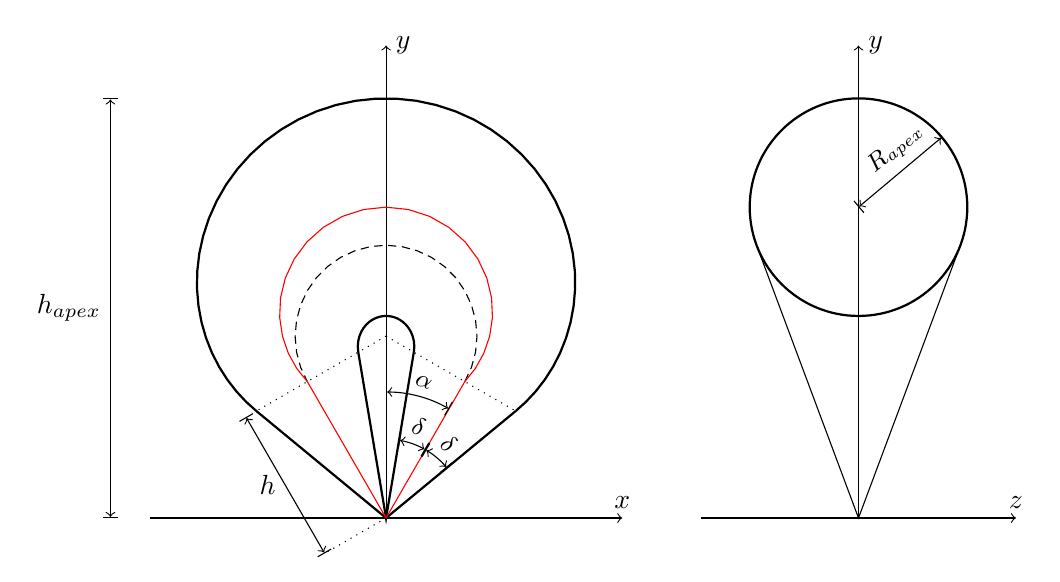
\begin{tikzpicture}
    \def\h{2}
    \def\palpha{30}
    \def\pkappa{0.35}
    
    \def\b{(\h / cos(\palpha))}
    \def\prho{(\h * tan(\palpha))}
    \def\pdelta{asin(\pkappa)}
    
    \def\Xnull{((\prho + \b * \pkappa^2 * sin(\x)) / (1 - \pkappa^2))}
    \def\Rc{sqrt(\Xnull^2 + (\b^2 * \pkappa^2 - \prho^2)/(1 - \pkappa^2))}
    
    \begin{scope}
        % xy view
        \draw[->] (0, 0) -- (0, 6) node[right] {$y$};
        \draw[->] (-3, 0) -- (3, 0) node[above] {$x$};
        
        \draw[densely dashed, domain=-\palpha:180+\palpha] plot ({\prho * cos(\x)}, {\prho * sin(\x) + \b});
        
        \draw[thick] ({90+\palpha+\pdelta}:{\h/cos(\pdelta)}) -- (0, 0) -- ({90-\palpha-\pdelta}:{\h/cos(\pdelta)});
        \draw[thick] ({90+\palpha-\pdelta}:{\h/cos(\pdelta)}) -- (0, 0) -- ({90-\palpha+\pdelta}:{\h/cos(\pdelta)});
        
        % central axis
        \draw[red] (90+\palpha:\h) -- (0, 0) -- (90-\palpha:\h);
        \draw[red, domain=-\palpha:180+\palpha] plot ({\Xnull * cos(\x)}, {\Xnull * sin(\x) + \b});
        
        \draw[thick,domain=-\palpha:180+\palpha,samples=50] plot ({(\Xnull + \Rc) * cos(\x)}, {(\Xnull + \Rc) * sin(\x) + \b});
        \draw[thick,domain=-\palpha:180+\palpha] plot ({(\Xnull - \Rc) * cos(\x)}, {(\Xnull - \Rc) * sin(\x) + \b});
        
        \draw[dotted] (0, {\b}) -- ({90+\palpha+\pdelta}:{\h/cos(\pdelta)});
        \draw[dotted] (0, {\b}) -- ({90-\palpha-\pdelta}:{\h/cos(\pdelta)});
        
        % definitions of delta, alpha, h and h_apex
        \draw[|<->|] ({90-\palpha-\pdelta}:{\h*0.5}) arc ({90-\palpha-\pdelta}:{90-\palpha}:{\h*0.5}) node[midway, above, rotate={-\palpha - \pdelta/2}] {\small$\delta$};
        \draw[|<->|] ({90-\palpha+\pdelta}:{\h*0.5}) arc ({90-\palpha+\pdelta}:{90-\palpha}:{\h*0.5}) node[midway, above, rotate={-\palpha + \pdelta/2}] {\small$\delta$};
        
        \draw[|<->|] ({90}:{\h*0.8}) arc ({90}:{90-\palpha}:{\h*0.8}) node[midway, above, rotate={-\palpha + \pdelta/2}] {\small$\alpha$};
        
        \def\x{90}
        \draw[|<->|] (0, 0) ++ ({\palpha}:-0.9) -- node[left] {$h$} ++({90+\palpha}:{\h});
        \draw[dotted] (0, 0) -- ++ ({\palpha}:-0.9);
        
        \draw[|<->|] (-3.5, 0) -- node[left] {$h_\text{apex}$} (-3.5, {\b + \Xnull + \Rc});
    \end{scope}
    
    \begin{scope}[xshift=6cm]
        % yz view
        \draw[->] (0, 0) -- (0, 6) node[right] {$y$};
        \draw[->] (-2, 0) -- (2, 0) node[above] {$z$};
        
        % front
        \def\Xnull{((\prho + \b * \pkappa^2 * sin(\x)) / (1 - \pkappa^2))}
        \def\Rc{sqrt(\Xnull^2 + (\b^2 * \pkappa^2 - \prho^2)/(1 - \pkappa^2))}
        \def\x{90}
        
        \draw[thick](0, {\b + \Xnull}) circle (\Rc);
        
        \draw ({90-\pdelta}:{(\b + \Xnull) * cos(\pdelta)}) -- (0, 0) -- ({90+\pdelta}:{(\b + \Xnull) * cos(\pdelta)});
        
        % definition of R_apex
        \draw[|<->|] (0, {\b + \Xnull}) -- node[above,rotate=40,xshift=1.5mm] {\small $R_\text{apex}$} ++ (40:{\Rc});
    \end{scope}
\end{tikzpicture}
    \caption[Illustration of the \ac{GCS} model]{Illustration of the \ac{GCS} model and definition of parameters $h, h_\text{apex}$, $\alpha$, $\delta$ and $R_\text{apex}$. Adapted from \citet{Thernisien-2011-GCS}. In this example, the parameters are set to $\alpha = \SI{30}{\degree}$ and $\kappa = 0.35$. The left panel shows a side view of the \ac{CME} in the $xy$ plane, where the thick line marks the outer contour of the flux rope and the thin line corresponds to its central axis. The dotted lines mark the boundary between the front section and the legs. The dashed line is a circular arc around the central point, showing that the front section does not have a constant radius. The right panel shows a cut in the perpendicular $yz$ plane, where the cross section of the front is marked with a thick circle and the conical legs are indicated using the thin lines.}
    \label{fig:gcs_schematic}
\end{figure}

The \ac{GCS} geometry is constrained using 3 main parameters: The \ac{CME} apex height $h_\text{apex}$ (or, alternatively, the leg height $h$), the angular half width $\alpha$ of the \ac{CME}, and the so-called aspect ratio $\kappa$, which corresponds to the half angle $\delta$ of the leg cones:
\begin{equation}
    \kappa = \sin \delta
\end{equation}
Three additional parameters describe the orientation of the flux rope relative to the Sun: The heliographic latitude $\theta$, longitude $\phi$ (typically given in Stonyhurst or Carrington coordinates), and the tilt angle $\gamma$, which defines the rotation around the $y$ axis in \autoref{fig:gcs_schematic}. For a detailed description of the mathematical derivation of the \ac{GCS} model, please refer to \citet{Thernisien-2011-GCS}.

The \ac{GCS} model is typically employed in a forward modelling approach, i.e., the model is visually compared to coronagraph observations of a \ac{CME} and the input parameters are then iteratively adjusted by the scientist to achieve a good fit. This manual fitting process is ideally applied simultaneously to coronagraph images from multiple viewpoints, such as from the \ac{SOHO} and \ac{STEREO} spacecraft, to avoid ambiguity due to the line of sight effect. The resulting \ac{GCS} parameters for the best fit can then be used for further evaluation, e.g. as input parameters for further models. Additional properties of the flux rope, such as the radius at the apex $R_\text{apex}$ (see \autoref{fig:gcs_schematic}) can also be calculated from these parameters, as derived by \citep{Thernisien-2011-GCS}. When applied to a sequence of consecutive images, the \ac{CME} kinematics can also be reconstructed.

The original implementation of the \ac{GCS} model in the \ac{IDL}\footnote{\url{https://www.l3harrisgeospatial.com/Software-Technology/IDL}} and a corresponding \ac{GUI} were developed by \citet{Thernisien-2006-GCS} and is included in the SolarSoft software package \citep{Freeland-1998-SolarSoft} under the name \texttt{scraytrace}\footnote{\url{https://hesperia.gsfc.nasa.gov/ssw/stereo/secchi/idl/scraytrace}}.
Using this implementation requires a local installation of SolarSoft and the corresponding database (SSWDB), which includes coronagraph images and calibration data. Obtaining and installing all these components is quite involved for scientists that are not familiar \ac{IDL} and SolarSoft, and the \ac{GCS} implementation is only partially documented and not very flexible, as it was initially hard-coded to work with only \ac{STEREO}-A and -B data, with support for \ac{SOHO} being manually added later.

As described e.g. in the detailed review by \citet{Burrell-2018}, the Python programming language is becoming increasingly popular in the solar and heliospheric physics community, and consequently, various open source software libraries to assist with the associated data analysis are available. Python is a modern, general-purpose object-oriented programming language that is easy to learn and emphasizes code readability. According to the TIOBE Programming Community Index\footnote{\url{https://www.tiobe.com/tiobe-index/}}, it has recently surpassed Java as the second most popular programming language in the world, and in contrast to \ac{IDL}, it is open source software (OSS) and available free of charge on all major operating systems.

\textit{SunPy}, a library \citep{sunpy_community2020} for working with solar images from various missions, is one of the most widely-used Python toolkits for solar physics. However, it does not yet provide any models for \ac{CME} reconstruction in coronagraph images.
Thus, I have developed an open source Python implementation of the \ac{GCS} model and a simple corresponding \ac{GUI} application, based on \textit{SunPy}. It can be used both as as a standalone application as well as integrated into existing Python-based plotting routines. The source code is available on GitHub at \url{https://github.com/johan12345/gcs_python}, and is also mirrored at Kiel University under \url{https://gitlab.physik.uni-kiel.de/ET/gcs_python}. It can be easily installed with Python's \texttt{pip} package manager as follows:
\begin{minted}{bash}
pip3 install git+https://github.com/johan12345/gcs_python.git
\end{minted}
(provided that Python 3.7 or above is already installed).

The following sections will describe the design and usage of this software package, and its validation against the original \ac{IDL} version.

\section{GCS geometry}

The basic \ac{GCS} geometry is implemented in the \texttt{gcs.geometry} module. This code is a close translation of the corresponding \ac{IDL} routines from SolarSoft. Two basic functions are provided to calculate the geometry of the \ac{GCS} structure based on the input parameters: The \texttt{skeleton} function (based on \texttt{shellskeleton.pro} in SolarSoft) calculates the shape of the central axis of the flux rope (thin solid line in \autoref{fig:gcs_schematic}), which consists of two straight segments in the legs and a curved segment in the front. The desired resolution, i.e. the number of vertices along each part of the curve, can be passed to the function.
In addition to the the points along the axis, the \texttt{skeleton} function also provides the radius of the circular shell at each point, and the orientation of these circles (i.e. the the tangent vector to the central axis in the $xy$ plane), which are necessary for the following generation of the outer shell.
The \verb|gcs_mesh| function (based on \texttt{cmecloud.pro} in SolarSoft) then uses the output of the \texttt{skeleton} function to construct a 3D mesh by generating circles around each point of the central axis with the appropriate radius and orientation. The parameters of the \verb|gcs_mesh| function are the half angle $\alpha$, the \ac{CME} height $h_\text{apex}$, and the aspect ratio $\kappa$, as well as the desired numbers of vertices along the straight segments, along the front, and along each circle in the mesh.

\begin{figure}
	\centering
	%% Creator: Matplotlib, PGF backend
%%
%% To include the figure in your LaTeX document, write
%%   \input{<filename>.pgf}
%%
%% Make sure the required packages are loaded in your preamble
%%   \usepackage{pgf}
%%
%% and, on pdftex
%%   \usepackage[utf8]{inputenc}\DeclareUnicodeCharacter{2212}{-}
%%
%% or, on luatex and xetex
%%   \usepackage{unicode-math}
%%
%% Figures using additional raster images can only be included by \input if
%% they are in the same directory as the main LaTeX file. For loading figures
%% from other directories you can use the `import` package
%%   \usepackage{import}
%%
%% and then include the figures with
%%   \import{<path to file>}{<filename>.pgf}
%%
%% Matplotlib used the following preamble
%%   \usepackage{fontspec}
%%
\begingroup%
\makeatletter%
\begin{pgfpicture}%
\pgfpathrectangle{\pgfpointorigin}{\pgfqpoint{5.000000in}{2.300000in}}%
\pgfusepath{use as bounding box, clip}%
\begin{pgfscope}%
\pgfsetbuttcap%
\pgfsetmiterjoin%
\definecolor{currentfill}{rgb}{1.000000,1.000000,1.000000}%
\pgfsetfillcolor{currentfill}%
\pgfsetlinewidth{0.000000pt}%
\definecolor{currentstroke}{rgb}{1.000000,1.000000,1.000000}%
\pgfsetstrokecolor{currentstroke}%
\pgfsetdash{}{0pt}%
\pgfpathmoveto{\pgfqpoint{0.000000in}{0.000000in}}%
\pgfpathlineto{\pgfqpoint{5.000000in}{0.000000in}}%
\pgfpathlineto{\pgfqpoint{5.000000in}{2.300000in}}%
\pgfpathlineto{\pgfqpoint{0.000000in}{2.300000in}}%
\pgfpathclose%
\pgfusepath{fill}%
\end{pgfscope}%
\begin{pgfscope}%
\pgfsetbuttcap%
\pgfsetmiterjoin%
\definecolor{currentfill}{rgb}{1.000000,1.000000,1.000000}%
\pgfsetfillcolor{currentfill}%
\pgfsetlinewidth{0.000000pt}%
\definecolor{currentstroke}{rgb}{0.000000,0.000000,0.000000}%
\pgfsetstrokecolor{currentstroke}%
\pgfsetstrokeopacity{0.000000}%
\pgfsetdash{}{0pt}%
\pgfpathmoveto{\pgfqpoint{0.328551in}{0.328551in}}%
\pgfpathlineto{\pgfqpoint{2.514276in}{0.328551in}}%
\pgfpathlineto{\pgfqpoint{2.514276in}{2.150000in}}%
\pgfpathlineto{\pgfqpoint{0.328551in}{2.150000in}}%
\pgfpathclose%
\pgfusepath{fill}%
\end{pgfscope}%
\begin{pgfscope}%
\pgfpathrectangle{\pgfqpoint{0.328551in}{0.328551in}}{\pgfqpoint{2.185724in}{1.821449in}}%
\pgfusepath{clip}%
\pgfsetbuttcap%
\pgfsetroundjoin%
\definecolor{currentfill}{rgb}{0.121569,0.466667,0.705882}%
\pgfsetfillcolor{currentfill}%
\pgfsetlinewidth{1.003750pt}%
\definecolor{currentstroke}{rgb}{0.121569,0.466667,0.705882}%
\pgfsetstrokecolor{currentstroke}%
\pgfsetdash{}{0pt}%
\pgfsys@defobject{currentmarker}{\pgfqpoint{-0.003106in}{-0.003106in}}{\pgfqpoint{0.003106in}{0.003106in}}{%
\pgfpathmoveto{\pgfqpoint{0.000000in}{-0.003106in}}%
\pgfpathcurveto{\pgfqpoint{0.000824in}{-0.003106in}}{\pgfqpoint{0.001614in}{-0.002778in}}{\pgfqpoint{0.002196in}{-0.002196in}}%
\pgfpathcurveto{\pgfqpoint{0.002778in}{-0.001614in}}{\pgfqpoint{0.003106in}{-0.000824in}}{\pgfqpoint{0.003106in}{0.000000in}}%
\pgfpathcurveto{\pgfqpoint{0.003106in}{0.000824in}}{\pgfqpoint{0.002778in}{0.001614in}}{\pgfqpoint{0.002196in}{0.002196in}}%
\pgfpathcurveto{\pgfqpoint{0.001614in}{0.002778in}}{\pgfqpoint{0.000824in}{0.003106in}}{\pgfqpoint{0.000000in}{0.003106in}}%
\pgfpathcurveto{\pgfqpoint{-0.000824in}{0.003106in}}{\pgfqpoint{-0.001614in}{0.002778in}}{\pgfqpoint{-0.002196in}{0.002196in}}%
\pgfpathcurveto{\pgfqpoint{-0.002778in}{0.001614in}}{\pgfqpoint{-0.003106in}{0.000824in}}{\pgfqpoint{-0.003106in}{0.000000in}}%
\pgfpathcurveto{\pgfqpoint{-0.003106in}{-0.000824in}}{\pgfqpoint{-0.002778in}{-0.001614in}}{\pgfqpoint{-0.002196in}{-0.002196in}}%
\pgfpathcurveto{\pgfqpoint{-0.001614in}{-0.002778in}}{\pgfqpoint{-0.000824in}{-0.003106in}}{\pgfqpoint{0.000000in}{-0.003106in}}%
\pgfpathclose%
\pgfusepath{stroke,fill}%
}%
\begin{pgfscope}%
\pgfsys@transformshift{1.421413in}{0.411344in}%
\pgfsys@useobject{currentmarker}{}%
\end{pgfscope}%
\begin{pgfscope}%
\pgfsys@transformshift{1.421413in}{0.411344in}%
\pgfsys@useobject{currentmarker}{}%
\end{pgfscope}%
\begin{pgfscope}%
\pgfsys@transformshift{1.421413in}{0.411344in}%
\pgfsys@useobject{currentmarker}{}%
\end{pgfscope}%
\begin{pgfscope}%
\pgfsys@transformshift{1.421413in}{0.411344in}%
\pgfsys@useobject{currentmarker}{}%
\end{pgfscope}%
\begin{pgfscope}%
\pgfsys@transformshift{1.421413in}{0.411344in}%
\pgfsys@useobject{currentmarker}{}%
\end{pgfscope}%
\begin{pgfscope}%
\pgfsys@transformshift{1.421413in}{0.411344in}%
\pgfsys@useobject{currentmarker}{}%
\end{pgfscope}%
\begin{pgfscope}%
\pgfsys@transformshift{1.421413in}{0.411344in}%
\pgfsys@useobject{currentmarker}{}%
\end{pgfscope}%
\begin{pgfscope}%
\pgfsys@transformshift{1.421413in}{0.411344in}%
\pgfsys@useobject{currentmarker}{}%
\end{pgfscope}%
\begin{pgfscope}%
\pgfsys@transformshift{1.421413in}{0.411344in}%
\pgfsys@useobject{currentmarker}{}%
\end{pgfscope}%
\begin{pgfscope}%
\pgfsys@transformshift{1.421413in}{0.411344in}%
\pgfsys@useobject{currentmarker}{}%
\end{pgfscope}%
\begin{pgfscope}%
\pgfsys@transformshift{1.421413in}{0.411344in}%
\pgfsys@useobject{currentmarker}{}%
\end{pgfscope}%
\begin{pgfscope}%
\pgfsys@transformshift{1.421413in}{0.411344in}%
\pgfsys@useobject{currentmarker}{}%
\end{pgfscope}%
\begin{pgfscope}%
\pgfsys@transformshift{1.421413in}{0.411344in}%
\pgfsys@useobject{currentmarker}{}%
\end{pgfscope}%
\begin{pgfscope}%
\pgfsys@transformshift{1.421413in}{0.411344in}%
\pgfsys@useobject{currentmarker}{}%
\end{pgfscope}%
\begin{pgfscope}%
\pgfsys@transformshift{1.421413in}{0.411344in}%
\pgfsys@useobject{currentmarker}{}%
\end{pgfscope}%
\begin{pgfscope}%
\pgfsys@transformshift{1.421413in}{0.411344in}%
\pgfsys@useobject{currentmarker}{}%
\end{pgfscope}%
\begin{pgfscope}%
\pgfsys@transformshift{1.421413in}{0.411344in}%
\pgfsys@useobject{currentmarker}{}%
\end{pgfscope}%
\begin{pgfscope}%
\pgfsys@transformshift{1.421413in}{0.411344in}%
\pgfsys@useobject{currentmarker}{}%
\end{pgfscope}%
\begin{pgfscope}%
\pgfsys@transformshift{1.421413in}{0.411344in}%
\pgfsys@useobject{currentmarker}{}%
\end{pgfscope}%
\begin{pgfscope}%
\pgfsys@transformshift{1.421413in}{0.411344in}%
\pgfsys@useobject{currentmarker}{}%
\end{pgfscope}%
\begin{pgfscope}%
\pgfsys@transformshift{1.455967in}{0.471192in}%
\pgfsys@useobject{currentmarker}{}%
\end{pgfscope}%
\begin{pgfscope}%
\pgfsys@transformshift{1.463227in}{0.467000in}%
\pgfsys@useobject{currentmarker}{}%
\end{pgfscope}%
\begin{pgfscope}%
\pgfsys@transformshift{1.469701in}{0.463263in}%
\pgfsys@useobject{currentmarker}{}%
\end{pgfscope}%
\begin{pgfscope}%
\pgfsys@transformshift{1.474687in}{0.460384in}%
\pgfsys@useobject{currentmarker}{}%
\end{pgfscope}%
\begin{pgfscope}%
\pgfsys@transformshift{1.477643in}{0.458677in}%
\pgfsys@useobject{currentmarker}{}%
\end{pgfscope}%
\begin{pgfscope}%
\pgfsys@transformshift{1.478251in}{0.458326in}%
\pgfsys@useobject{currentmarker}{}%
\end{pgfscope}%
\begin{pgfscope}%
\pgfsys@transformshift{1.476444in}{0.459369in}%
\pgfsys@useobject{currentmarker}{}%
\end{pgfscope}%
\begin{pgfscope}%
\pgfsys@transformshift{1.472418in}{0.461694in}%
\pgfsys@useobject{currentmarker}{}%
\end{pgfscope}%
\begin{pgfscope}%
\pgfsys@transformshift{1.466609in}{0.465048in}%
\pgfsys@useobject{currentmarker}{}%
\end{pgfscope}%
\begin{pgfscope}%
\pgfsys@transformshift{1.459647in}{0.469067in}%
\pgfsys@useobject{currentmarker}{}%
\end{pgfscope}%
\begin{pgfscope}%
\pgfsys@transformshift{1.452286in}{0.473317in}%
\pgfsys@useobject{currentmarker}{}%
\end{pgfscope}%
\begin{pgfscope}%
\pgfsys@transformshift{1.445324in}{0.477337in}%
\pgfsys@useobject{currentmarker}{}%
\end{pgfscope}%
\begin{pgfscope}%
\pgfsys@transformshift{1.439515in}{0.480691in}%
\pgfsys@useobject{currentmarker}{}%
\end{pgfscope}%
\begin{pgfscope}%
\pgfsys@transformshift{1.435489in}{0.483015in}%
\pgfsys@useobject{currentmarker}{}%
\end{pgfscope}%
\begin{pgfscope}%
\pgfsys@transformshift{1.433682in}{0.484058in}%
\pgfsys@useobject{currentmarker}{}%
\end{pgfscope}%
\begin{pgfscope}%
\pgfsys@transformshift{1.434290in}{0.483707in}%
\pgfsys@useobject{currentmarker}{}%
\end{pgfscope}%
\begin{pgfscope}%
\pgfsys@transformshift{1.437247in}{0.482000in}%
\pgfsys@useobject{currentmarker}{}%
\end{pgfscope}%
\begin{pgfscope}%
\pgfsys@transformshift{1.442232in}{0.479122in}%
\pgfsys@useobject{currentmarker}{}%
\end{pgfscope}%
\begin{pgfscope}%
\pgfsys@transformshift{1.448706in}{0.475384in}%
\pgfsys@useobject{currentmarker}{}%
\end{pgfscope}%
\begin{pgfscope}%
\pgfsys@transformshift{1.455967in}{0.471192in}%
\pgfsys@useobject{currentmarker}{}%
\end{pgfscope}%
\begin{pgfscope}%
\pgfsys@transformshift{1.490520in}{0.531040in}%
\pgfsys@useobject{currentmarker}{}%
\end{pgfscope}%
\begin{pgfscope}%
\pgfsys@transformshift{1.505041in}{0.522656in}%
\pgfsys@useobject{currentmarker}{}%
\end{pgfscope}%
\begin{pgfscope}%
\pgfsys@transformshift{1.517989in}{0.515181in}%
\pgfsys@useobject{currentmarker}{}%
\end{pgfscope}%
\begin{pgfscope}%
\pgfsys@transformshift{1.527960in}{0.509424in}%
\pgfsys@useobject{currentmarker}{}%
\end{pgfscope}%
\begin{pgfscope}%
\pgfsys@transformshift{1.533874in}{0.506010in}%
\pgfsys@useobject{currentmarker}{}%
\end{pgfscope}%
\begin{pgfscope}%
\pgfsys@transformshift{1.535089in}{0.505308in}%
\pgfsys@useobject{currentmarker}{}%
\end{pgfscope}%
\begin{pgfscope}%
\pgfsys@transformshift{1.531475in}{0.507395in}%
\pgfsys@useobject{currentmarker}{}%
\end{pgfscope}%
\begin{pgfscope}%
\pgfsys@transformshift{1.523423in}{0.512044in}%
\pgfsys@useobject{currentmarker}{}%
\end{pgfscope}%
\begin{pgfscope}%
\pgfsys@transformshift{1.511805in}{0.518751in}%
\pgfsys@useobject{currentmarker}{}%
\end{pgfscope}%
\begin{pgfscope}%
\pgfsys@transformshift{1.497881in}{0.526790in}%
\pgfsys@useobject{currentmarker}{}%
\end{pgfscope}%
\begin{pgfscope}%
\pgfsys@transformshift{1.483159in}{0.535290in}%
\pgfsys@useobject{currentmarker}{}%
\end{pgfscope}%
\begin{pgfscope}%
\pgfsys@transformshift{1.469234in}{0.543329in}%
\pgfsys@useobject{currentmarker}{}%
\end{pgfscope}%
\begin{pgfscope}%
\pgfsys@transformshift{1.457617in}{0.550037in}%
\pgfsys@useobject{currentmarker}{}%
\end{pgfscope}%
\begin{pgfscope}%
\pgfsys@transformshift{1.449564in}{0.554686in}%
\pgfsys@useobject{currentmarker}{}%
\end{pgfscope}%
\begin{pgfscope}%
\pgfsys@transformshift{1.445950in}{0.556773in}%
\pgfsys@useobject{currentmarker}{}%
\end{pgfscope}%
\begin{pgfscope}%
\pgfsys@transformshift{1.447166in}{0.556071in}%
\pgfsys@useobject{currentmarker}{}%
\end{pgfscope}%
\begin{pgfscope}%
\pgfsys@transformshift{1.453080in}{0.552656in}%
\pgfsys@useobject{currentmarker}{}%
\end{pgfscope}%
\begin{pgfscope}%
\pgfsys@transformshift{1.463051in}{0.546900in}%
\pgfsys@useobject{currentmarker}{}%
\end{pgfscope}%
\begin{pgfscope}%
\pgfsys@transformshift{1.475999in}{0.539424in}%
\pgfsys@useobject{currentmarker}{}%
\end{pgfscope}%
\begin{pgfscope}%
\pgfsys@transformshift{1.490520in}{0.531040in}%
\pgfsys@useobject{currentmarker}{}%
\end{pgfscope}%
\begin{pgfscope}%
\pgfsys@transformshift{1.525073in}{0.590888in}%
\pgfsys@useobject{currentmarker}{}%
\end{pgfscope}%
\begin{pgfscope}%
\pgfsys@transformshift{1.546855in}{0.578312in}%
\pgfsys@useobject{currentmarker}{}%
\end{pgfscope}%
\begin{pgfscope}%
\pgfsys@transformshift{1.566277in}{0.567099in}%
\pgfsys@useobject{currentmarker}{}%
\end{pgfscope}%
\begin{pgfscope}%
\pgfsys@transformshift{1.581233in}{0.558464in}%
\pgfsys@useobject{currentmarker}{}%
\end{pgfscope}%
\begin{pgfscope}%
\pgfsys@transformshift{1.590104in}{0.553343in}%
\pgfsys@useobject{currentmarker}{}%
\end{pgfscope}%
\begin{pgfscope}%
\pgfsys@transformshift{1.591928in}{0.552290in}%
\pgfsys@useobject{currentmarker}{}%
\end{pgfscope}%
\begin{pgfscope}%
\pgfsys@transformshift{1.586506in}{0.555420in}%
\pgfsys@useobject{currentmarker}{}%
\end{pgfscope}%
\begin{pgfscope}%
\pgfsys@transformshift{1.574428in}{0.562393in}%
\pgfsys@useobject{currentmarker}{}%
\end{pgfscope}%
\begin{pgfscope}%
\pgfsys@transformshift{1.557001in}{0.572455in}%
\pgfsys@useobject{currentmarker}{}%
\end{pgfscope}%
\begin{pgfscope}%
\pgfsys@transformshift{1.536115in}{0.584513in}%
\pgfsys@useobject{currentmarker}{}%
\end{pgfscope}%
\begin{pgfscope}%
\pgfsys@transformshift{1.514032in}{0.597263in}%
\pgfsys@useobject{currentmarker}{}%
\end{pgfscope}%
\begin{pgfscope}%
\pgfsys@transformshift{1.493145in}{0.609322in}%
\pgfsys@useobject{currentmarker}{}%
\end{pgfscope}%
\begin{pgfscope}%
\pgfsys@transformshift{1.475718in}{0.619383in}%
\pgfsys@useobject{currentmarker}{}%
\end{pgfscope}%
\begin{pgfscope}%
\pgfsys@transformshift{1.463640in}{0.626357in}%
\pgfsys@useobject{currentmarker}{}%
\end{pgfscope}%
\begin{pgfscope}%
\pgfsys@transformshift{1.458219in}{0.629487in}%
\pgfsys@useobject{currentmarker}{}%
\end{pgfscope}%
\begin{pgfscope}%
\pgfsys@transformshift{1.460042in}{0.628434in}%
\pgfsys@useobject{currentmarker}{}%
\end{pgfscope}%
\begin{pgfscope}%
\pgfsys@transformshift{1.468913in}{0.623312in}%
\pgfsys@useobject{currentmarker}{}%
\end{pgfscope}%
\begin{pgfscope}%
\pgfsys@transformshift{1.483870in}{0.614677in}%
\pgfsys@useobject{currentmarker}{}%
\end{pgfscope}%
\begin{pgfscope}%
\pgfsys@transformshift{1.503291in}{0.603464in}%
\pgfsys@useobject{currentmarker}{}%
\end{pgfscope}%
\begin{pgfscope}%
\pgfsys@transformshift{1.525073in}{0.590888in}%
\pgfsys@useobject{currentmarker}{}%
\end{pgfscope}%
\begin{pgfscope}%
\pgfsys@transformshift{1.559626in}{0.650736in}%
\pgfsys@useobject{currentmarker}{}%
\end{pgfscope}%
\begin{pgfscope}%
\pgfsys@transformshift{1.588669in}{0.633969in}%
\pgfsys@useobject{currentmarker}{}%
\end{pgfscope}%
\begin{pgfscope}%
\pgfsys@transformshift{1.614564in}{0.619018in}%
\pgfsys@useobject{currentmarker}{}%
\end{pgfscope}%
\begin{pgfscope}%
\pgfsys@transformshift{1.634506in}{0.607504in}%
\pgfsys@useobject{currentmarker}{}%
\end{pgfscope}%
\begin{pgfscope}%
\pgfsys@transformshift{1.646334in}{0.600676in}%
\pgfsys@useobject{currentmarker}{}%
\end{pgfscope}%
\begin{pgfscope}%
\pgfsys@transformshift{1.648766in}{0.599272in}%
\pgfsys@useobject{currentmarker}{}%
\end{pgfscope}%
\begin{pgfscope}%
\pgfsys@transformshift{1.641537in}{0.603445in}%
\pgfsys@useobject{currentmarker}{}%
\end{pgfscope}%
\begin{pgfscope}%
\pgfsys@transformshift{1.625433in}{0.612743in}%
\pgfsys@useobject{currentmarker}{}%
\end{pgfscope}%
\begin{pgfscope}%
\pgfsys@transformshift{1.602197in}{0.626158in}%
\pgfsys@useobject{currentmarker}{}%
\end{pgfscope}%
\begin{pgfscope}%
\pgfsys@transformshift{1.574349in}{0.642237in}%
\pgfsys@useobject{currentmarker}{}%
\end{pgfscope}%
\begin{pgfscope}%
\pgfsys@transformshift{1.544904in}{0.659236in}%
\pgfsys@useobject{currentmarker}{}%
\end{pgfscope}%
\begin{pgfscope}%
\pgfsys@transformshift{1.517055in}{0.675315in}%
\pgfsys@useobject{currentmarker}{}%
\end{pgfscope}%
\begin{pgfscope}%
\pgfsys@transformshift{1.493820in}{0.688730in}%
\pgfsys@useobject{currentmarker}{}%
\end{pgfscope}%
\begin{pgfscope}%
\pgfsys@transformshift{1.477715in}{0.698028in}%
\pgfsys@useobject{currentmarker}{}%
\end{pgfscope}%
\begin{pgfscope}%
\pgfsys@transformshift{1.470487in}{0.702201in}%
\pgfsys@useobject{currentmarker}{}%
\end{pgfscope}%
\begin{pgfscope}%
\pgfsys@transformshift{1.472919in}{0.700797in}%
\pgfsys@useobject{currentmarker}{}%
\end{pgfscope}%
\begin{pgfscope}%
\pgfsys@transformshift{1.484746in}{0.693968in}%
\pgfsys@useobject{currentmarker}{}%
\end{pgfscope}%
\begin{pgfscope}%
\pgfsys@transformshift{1.504688in}{0.682455in}%
\pgfsys@useobject{currentmarker}{}%
\end{pgfscope}%
\begin{pgfscope}%
\pgfsys@transformshift{1.530584in}{0.667504in}%
\pgfsys@useobject{currentmarker}{}%
\end{pgfscope}%
\begin{pgfscope}%
\pgfsys@transformshift{1.559626in}{0.650736in}%
\pgfsys@useobject{currentmarker}{}%
\end{pgfscope}%
\begin{pgfscope}%
\pgfsys@transformshift{1.594180in}{0.710584in}%
\pgfsys@useobject{currentmarker}{}%
\end{pgfscope}%
\begin{pgfscope}%
\pgfsys@transformshift{1.630483in}{0.689625in}%
\pgfsys@useobject{currentmarker}{}%
\end{pgfscope}%
\begin{pgfscope}%
\pgfsys@transformshift{1.662852in}{0.670936in}%
\pgfsys@useobject{currentmarker}{}%
\end{pgfscope}%
\begin{pgfscope}%
\pgfsys@transformshift{1.687780in}{0.656544in}%
\pgfsys@useobject{currentmarker}{}%
\end{pgfscope}%
\begin{pgfscope}%
\pgfsys@transformshift{1.702564in}{0.648009in}%
\pgfsys@useobject{currentmarker}{}%
\end{pgfscope}%
\begin{pgfscope}%
\pgfsys@transformshift{1.705604in}{0.646254in}%
\pgfsys@useobject{currentmarker}{}%
\end{pgfscope}%
\begin{pgfscope}%
\pgfsys@transformshift{1.696568in}{0.651470in}%
\pgfsys@useobject{currentmarker}{}%
\end{pgfscope}%
\begin{pgfscope}%
\pgfsys@transformshift{1.676438in}{0.663093in}%
\pgfsys@useobject{currentmarker}{}%
\end{pgfscope}%
\begin{pgfscope}%
\pgfsys@transformshift{1.647393in}{0.679861in}%
\pgfsys@useobject{currentmarker}{}%
\end{pgfscope}%
\begin{pgfscope}%
\pgfsys@transformshift{1.612582in}{0.699960in}%
\pgfsys@useobject{currentmarker}{}%
\end{pgfscope}%
\begin{pgfscope}%
\pgfsys@transformshift{1.575777in}{0.721209in}%
\pgfsys@useobject{currentmarker}{}%
\end{pgfscope}%
\begin{pgfscope}%
\pgfsys@transformshift{1.540966in}{0.741307in}%
\pgfsys@useobject{currentmarker}{}%
\end{pgfscope}%
\begin{pgfscope}%
\pgfsys@transformshift{1.511921in}{0.758076in}%
\pgfsys@useobject{currentmarker}{}%
\end{pgfscope}%
\begin{pgfscope}%
\pgfsys@transformshift{1.491791in}{0.769699in}%
\pgfsys@useobject{currentmarker}{}%
\end{pgfscope}%
\begin{pgfscope}%
\pgfsys@transformshift{1.482756in}{0.774915in}%
\pgfsys@useobject{currentmarker}{}%
\end{pgfscope}%
\begin{pgfscope}%
\pgfsys@transformshift{1.485795in}{0.773160in}%
\pgfsys@useobject{currentmarker}{}%
\end{pgfscope}%
\begin{pgfscope}%
\pgfsys@transformshift{1.500580in}{0.764624in}%
\pgfsys@useobject{currentmarker}{}%
\end{pgfscope}%
\begin{pgfscope}%
\pgfsys@transformshift{1.525507in}{0.750232in}%
\pgfsys@useobject{currentmarker}{}%
\end{pgfscope}%
\begin{pgfscope}%
\pgfsys@transformshift{1.557876in}{0.731544in}%
\pgfsys@useobject{currentmarker}{}%
\end{pgfscope}%
\begin{pgfscope}%
\pgfsys@transformshift{1.594180in}{0.710584in}%
\pgfsys@useobject{currentmarker}{}%
\end{pgfscope}%
\begin{pgfscope}%
\pgfsys@transformshift{1.628733in}{0.770432in}%
\pgfsys@useobject{currentmarker}{}%
\end{pgfscope}%
\begin{pgfscope}%
\pgfsys@transformshift{1.672297in}{0.745281in}%
\pgfsys@useobject{currentmarker}{}%
\end{pgfscope}%
\begin{pgfscope}%
\pgfsys@transformshift{1.711140in}{0.722855in}%
\pgfsys@useobject{currentmarker}{}%
\end{pgfscope}%
\begin{pgfscope}%
\pgfsys@transformshift{1.741053in}{0.705584in}%
\pgfsys@useobject{currentmarker}{}%
\end{pgfscope}%
\begin{pgfscope}%
\pgfsys@transformshift{1.758794in}{0.695341in}%
\pgfsys@useobject{currentmarker}{}%
\end{pgfscope}%
\begin{pgfscope}%
\pgfsys@transformshift{1.762442in}{0.693236in}%
\pgfsys@useobject{currentmarker}{}%
\end{pgfscope}%
\begin{pgfscope}%
\pgfsys@transformshift{1.751600in}{0.699495in}%
\pgfsys@useobject{currentmarker}{}%
\end{pgfscope}%
\begin{pgfscope}%
\pgfsys@transformshift{1.727443in}{0.713442in}%
\pgfsys@useobject{currentmarker}{}%
\end{pgfscope}%
\begin{pgfscope}%
\pgfsys@transformshift{1.692589in}{0.733565in}%
\pgfsys@useobject{currentmarker}{}%
\end{pgfscope}%
\begin{pgfscope}%
\pgfsys@transformshift{1.650816in}{0.757683in}%
\pgfsys@useobject{currentmarker}{}%
\end{pgfscope}%
\begin{pgfscope}%
\pgfsys@transformshift{1.606650in}{0.783182in}%
\pgfsys@useobject{currentmarker}{}%
\end{pgfscope}%
\begin{pgfscope}%
\pgfsys@transformshift{1.564877in}{0.807300in}%
\pgfsys@useobject{currentmarker}{}%
\end{pgfscope}%
\begin{pgfscope}%
\pgfsys@transformshift{1.530023in}{0.827423in}%
\pgfsys@useobject{currentmarker}{}%
\end{pgfscope}%
\begin{pgfscope}%
\pgfsys@transformshift{1.505866in}{0.841369in}%
\pgfsys@useobject{currentmarker}{}%
\end{pgfscope}%
\begin{pgfscope}%
\pgfsys@transformshift{1.495024in}{0.847629in}%
\pgfsys@useobject{currentmarker}{}%
\end{pgfscope}%
\begin{pgfscope}%
\pgfsys@transformshift{1.498671in}{0.845523in}%
\pgfsys@useobject{currentmarker}{}%
\end{pgfscope}%
\begin{pgfscope}%
\pgfsys@transformshift{1.516413in}{0.835280in}%
\pgfsys@useobject{currentmarker}{}%
\end{pgfscope}%
\begin{pgfscope}%
\pgfsys@transformshift{1.546326in}{0.818010in}%
\pgfsys@useobject{currentmarker}{}%
\end{pgfscope}%
\begin{pgfscope}%
\pgfsys@transformshift{1.585169in}{0.795584in}%
\pgfsys@useobject{currentmarker}{}%
\end{pgfscope}%
\begin{pgfscope}%
\pgfsys@transformshift{1.628733in}{0.770432in}%
\pgfsys@useobject{currentmarker}{}%
\end{pgfscope}%
\begin{pgfscope}%
\pgfsys@transformshift{1.663286in}{0.830280in}%
\pgfsys@useobject{currentmarker}{}%
\end{pgfscope}%
\begin{pgfscope}%
\pgfsys@transformshift{1.714111in}{0.800937in}%
\pgfsys@useobject{currentmarker}{}%
\end{pgfscope}%
\begin{pgfscope}%
\pgfsys@transformshift{1.759428in}{0.774773in}%
\pgfsys@useobject{currentmarker}{}%
\end{pgfscope}%
\begin{pgfscope}%
\pgfsys@transformshift{1.794326in}{0.754624in}%
\pgfsys@useobject{currentmarker}{}%
\end{pgfscope}%
\begin{pgfscope}%
\pgfsys@transformshift{1.815025in}{0.742674in}%
\pgfsys@useobject{currentmarker}{}%
\end{pgfscope}%
\begin{pgfscope}%
\pgfsys@transformshift{1.819280in}{0.740218in}%
\pgfsys@useobject{currentmarker}{}%
\end{pgfscope}%
\begin{pgfscope}%
\pgfsys@transformshift{1.806631in}{0.747521in}%
\pgfsys@useobject{currentmarker}{}%
\end{pgfscope}%
\begin{pgfscope}%
\pgfsys@transformshift{1.778448in}{0.763792in}%
\pgfsys@useobject{currentmarker}{}%
\end{pgfscope}%
\begin{pgfscope}%
\pgfsys@transformshift{1.737785in}{0.787268in}%
\pgfsys@useobject{currentmarker}{}%
\end{pgfscope}%
\begin{pgfscope}%
\pgfsys@transformshift{1.689050in}{0.815406in}%
\pgfsys@useobject{currentmarker}{}%
\end{pgfscope}%
\begin{pgfscope}%
\pgfsys@transformshift{1.637523in}{0.845155in}%
\pgfsys@useobject{currentmarker}{}%
\end{pgfscope}%
\begin{pgfscope}%
\pgfsys@transformshift{1.588787in}{0.873293in}%
\pgfsys@useobject{currentmarker}{}%
\end{pgfscope}%
\begin{pgfscope}%
\pgfsys@transformshift{1.548125in}{0.896769in}%
\pgfsys@useobject{currentmarker}{}%
\end{pgfscope}%
\begin{pgfscope}%
\pgfsys@transformshift{1.519942in}{0.913040in}%
\pgfsys@useobject{currentmarker}{}%
\end{pgfscope}%
\begin{pgfscope}%
\pgfsys@transformshift{1.507293in}{0.920343in}%
\pgfsys@useobject{currentmarker}{}%
\end{pgfscope}%
\begin{pgfscope}%
\pgfsys@transformshift{1.511548in}{0.917887in}%
\pgfsys@useobject{currentmarker}{}%
\end{pgfscope}%
\begin{pgfscope}%
\pgfsys@transformshift{1.532246in}{0.905936in}%
\pgfsys@useobject{currentmarker}{}%
\end{pgfscope}%
\begin{pgfscope}%
\pgfsys@transformshift{1.567145in}{0.885788in}%
\pgfsys@useobject{currentmarker}{}%
\end{pgfscope}%
\begin{pgfscope}%
\pgfsys@transformshift{1.612462in}{0.859624in}%
\pgfsys@useobject{currentmarker}{}%
\end{pgfscope}%
\begin{pgfscope}%
\pgfsys@transformshift{1.663286in}{0.830280in}%
\pgfsys@useobject{currentmarker}{}%
\end{pgfscope}%
\begin{pgfscope}%
\pgfsys@transformshift{1.697840in}{0.890128in}%
\pgfsys@useobject{currentmarker}{}%
\end{pgfscope}%
\begin{pgfscope}%
\pgfsys@transformshift{1.755925in}{0.856593in}%
\pgfsys@useobject{currentmarker}{}%
\end{pgfscope}%
\begin{pgfscope}%
\pgfsys@transformshift{1.807716in}{0.826692in}%
\pgfsys@useobject{currentmarker}{}%
\end{pgfscope}%
\begin{pgfscope}%
\pgfsys@transformshift{1.847600in}{0.803664in}%
\pgfsys@useobject{currentmarker}{}%
\end{pgfscope}%
\begin{pgfscope}%
\pgfsys@transformshift{1.871255in}{0.790007in}%
\pgfsys@useobject{currentmarker}{}%
\end{pgfscope}%
\begin{pgfscope}%
\pgfsys@transformshift{1.876118in}{0.787199in}%
\pgfsys@useobject{currentmarker}{}%
\end{pgfscope}%
\begin{pgfscope}%
\pgfsys@transformshift{1.861662in}{0.795546in}%
\pgfsys@useobject{currentmarker}{}%
\end{pgfscope}%
\begin{pgfscope}%
\pgfsys@transformshift{1.829453in}{0.814142in}%
\pgfsys@useobject{currentmarker}{}%
\end{pgfscope}%
\begin{pgfscope}%
\pgfsys@transformshift{1.782981in}{0.840972in}%
\pgfsys@useobject{currentmarker}{}%
\end{pgfscope}%
\begin{pgfscope}%
\pgfsys@transformshift{1.727284in}{0.873129in}%
\pgfsys@useobject{currentmarker}{}%
\end{pgfscope}%
\begin{pgfscope}%
\pgfsys@transformshift{1.668395in}{0.907128in}%
\pgfsys@useobject{currentmarker}{}%
\end{pgfscope}%
\begin{pgfscope}%
\pgfsys@transformshift{1.612698in}{0.939285in}%
\pgfsys@useobject{currentmarker}{}%
\end{pgfscope}%
\begin{pgfscope}%
\pgfsys@transformshift{1.566226in}{0.966115in}%
\pgfsys@useobject{currentmarker}{}%
\end{pgfscope}%
\begin{pgfscope}%
\pgfsys@transformshift{1.534017in}{0.984711in}%
\pgfsys@useobject{currentmarker}{}%
\end{pgfscope}%
\begin{pgfscope}%
\pgfsys@transformshift{1.519561in}{0.993058in}%
\pgfsys@useobject{currentmarker}{}%
\end{pgfscope}%
\begin{pgfscope}%
\pgfsys@transformshift{1.524424in}{0.990250in}%
\pgfsys@useobject{currentmarker}{}%
\end{pgfscope}%
\begin{pgfscope}%
\pgfsys@transformshift{1.548079in}{0.976593in}%
\pgfsys@useobject{currentmarker}{}%
\end{pgfscope}%
\begin{pgfscope}%
\pgfsys@transformshift{1.587963in}{0.953565in}%
\pgfsys@useobject{currentmarker}{}%
\end{pgfscope}%
\begin{pgfscope}%
\pgfsys@transformshift{1.639754in}{0.923664in}%
\pgfsys@useobject{currentmarker}{}%
\end{pgfscope}%
\begin{pgfscope}%
\pgfsys@transformshift{1.697840in}{0.890128in}%
\pgfsys@useobject{currentmarker}{}%
\end{pgfscope}%
\begin{pgfscope}%
\pgfsys@transformshift{1.732393in}{0.949977in}%
\pgfsys@useobject{currentmarker}{}%
\end{pgfscope}%
\begin{pgfscope}%
\pgfsys@transformshift{1.797739in}{0.912249in}%
\pgfsys@useobject{currentmarker}{}%
\end{pgfscope}%
\begin{pgfscope}%
\pgfsys@transformshift{1.856003in}{0.878610in}%
\pgfsys@useobject{currentmarker}{}%
\end{pgfscope}%
\begin{pgfscope}%
\pgfsys@transformshift{1.900873in}{0.852704in}%
\pgfsys@useobject{currentmarker}{}%
\end{pgfscope}%
\begin{pgfscope}%
\pgfsys@transformshift{1.927485in}{0.837340in}%
\pgfsys@useobject{currentmarker}{}%
\end{pgfscope}%
\begin{pgfscope}%
\pgfsys@transformshift{1.932956in}{0.834181in}%
\pgfsys@useobject{currentmarker}{}%
\end{pgfscope}%
\begin{pgfscope}%
\pgfsys@transformshift{1.916693in}{0.843571in}%
\pgfsys@useobject{currentmarker}{}%
\end{pgfscope}%
\begin{pgfscope}%
\pgfsys@transformshift{1.880458in}{0.864491in}%
\pgfsys@useobject{currentmarker}{}%
\end{pgfscope}%
\begin{pgfscope}%
\pgfsys@transformshift{1.828177in}{0.894675in}%
\pgfsys@useobject{currentmarker}{}%
\end{pgfscope}%
\begin{pgfscope}%
\pgfsys@transformshift{1.765518in}{0.930852in}%
\pgfsys@useobject{currentmarker}{}%
\end{pgfscope}%
\begin{pgfscope}%
\pgfsys@transformshift{1.699268in}{0.969101in}%
\pgfsys@useobject{currentmarker}{}%
\end{pgfscope}%
\begin{pgfscope}%
\pgfsys@transformshift{1.636608in}{1.005278in}%
\pgfsys@useobject{currentmarker}{}%
\end{pgfscope}%
\begin{pgfscope}%
\pgfsys@transformshift{1.584328in}{1.035462in}%
\pgfsys@useobject{currentmarker}{}%
\end{pgfscope}%
\begin{pgfscope}%
\pgfsys@transformshift{1.548093in}{1.056382in}%
\pgfsys@useobject{currentmarker}{}%
\end{pgfscope}%
\begin{pgfscope}%
\pgfsys@transformshift{1.531830in}{1.065772in}%
\pgfsys@useobject{currentmarker}{}%
\end{pgfscope}%
\begin{pgfscope}%
\pgfsys@transformshift{1.537301in}{1.062613in}%
\pgfsys@useobject{currentmarker}{}%
\end{pgfscope}%
\begin{pgfscope}%
\pgfsys@transformshift{1.563913in}{1.047249in}%
\pgfsys@useobject{currentmarker}{}%
\end{pgfscope}%
\begin{pgfscope}%
\pgfsys@transformshift{1.608782in}{1.021343in}%
\pgfsys@useobject{currentmarker}{}%
\end{pgfscope}%
\begin{pgfscope}%
\pgfsys@transformshift{1.667047in}{0.987704in}%
\pgfsys@useobject{currentmarker}{}%
\end{pgfscope}%
\begin{pgfscope}%
\pgfsys@transformshift{1.732393in}{0.949977in}%
\pgfsys@useobject{currentmarker}{}%
\end{pgfscope}%
\begin{pgfscope}%
\pgfsys@transformshift{1.759282in}{0.981317in}%
\pgfsys@useobject{currentmarker}{}%
\end{pgfscope}%
\begin{pgfscope}%
\pgfsys@transformshift{1.832830in}{0.949057in}%
\pgfsys@useobject{currentmarker}{}%
\end{pgfscope}%
\begin{pgfscope}%
\pgfsys@transformshift{1.898407in}{0.920292in}%
\pgfsys@useobject{currentmarker}{}%
\end{pgfscope}%
\begin{pgfscope}%
\pgfsys@transformshift{1.948908in}{0.898140in}%
\pgfsys@useobject{currentmarker}{}%
\end{pgfscope}%
\begin{pgfscope}%
\pgfsys@transformshift{1.978860in}{0.885002in}%
\pgfsys@useobject{currentmarker}{}%
\end{pgfscope}%
\begin{pgfscope}%
\pgfsys@transformshift{1.985017in}{0.882301in}%
\pgfsys@useobject{currentmarker}{}%
\end{pgfscope}%
\begin{pgfscope}%
\pgfsys@transformshift{1.966713in}{0.890330in}%
\pgfsys@useobject{currentmarker}{}%
\end{pgfscope}%
\begin{pgfscope}%
\pgfsys@transformshift{1.925930in}{0.908219in}%
\pgfsys@useobject{currentmarker}{}%
\end{pgfscope}%
\begin{pgfscope}%
\pgfsys@transformshift{1.867089in}{0.934029in}%
\pgfsys@useobject{currentmarker}{}%
\end{pgfscope}%
\begin{pgfscope}%
\pgfsys@transformshift{1.796565in}{0.964964in}%
\pgfsys@useobject{currentmarker}{}%
\end{pgfscope}%
\begin{pgfscope}%
\pgfsys@transformshift{1.722000in}{0.997671in}%
\pgfsys@useobject{currentmarker}{}%
\end{pgfscope}%
\begin{pgfscope}%
\pgfsys@transformshift{1.651476in}{1.028606in}%
\pgfsys@useobject{currentmarker}{}%
\end{pgfscope}%
\begin{pgfscope}%
\pgfsys@transformshift{1.592635in}{1.054416in}%
\pgfsys@useobject{currentmarker}{}%
\end{pgfscope}%
\begin{pgfscope}%
\pgfsys@transformshift{1.551852in}{1.072305in}%
\pgfsys@useobject{currentmarker}{}%
\end{pgfscope}%
\begin{pgfscope}%
\pgfsys@transformshift{1.533548in}{1.080334in}%
\pgfsys@useobject{currentmarker}{}%
\end{pgfscope}%
\begin{pgfscope}%
\pgfsys@transformshift{1.539705in}{1.077633in}%
\pgfsys@useobject{currentmarker}{}%
\end{pgfscope}%
\begin{pgfscope}%
\pgfsys@transformshift{1.569657in}{1.064495in}%
\pgfsys@useobject{currentmarker}{}%
\end{pgfscope}%
\begin{pgfscope}%
\pgfsys@transformshift{1.620158in}{1.042343in}%
\pgfsys@useobject{currentmarker}{}%
\end{pgfscope}%
\begin{pgfscope}%
\pgfsys@transformshift{1.685735in}{1.013578in}%
\pgfsys@useobject{currentmarker}{}%
\end{pgfscope}%
\begin{pgfscope}%
\pgfsys@transformshift{1.759282in}{0.981317in}%
\pgfsys@useobject{currentmarker}{}%
\end{pgfscope}%
\begin{pgfscope}%
\pgfsys@transformshift{1.783408in}{1.016297in}%
\pgfsys@useobject{currentmarker}{}%
\end{pgfscope}%
\begin{pgfscope}%
\pgfsys@transformshift{1.864763in}{0.990852in}%
\pgfsys@useobject{currentmarker}{}%
\end{pgfscope}%
\begin{pgfscope}%
\pgfsys@transformshift{1.937301in}{0.968163in}%
\pgfsys@useobject{currentmarker}{}%
\end{pgfscope}%
\begin{pgfscope}%
\pgfsys@transformshift{1.993163in}{0.950691in}%
\pgfsys@useobject{currentmarker}{}%
\end{pgfscope}%
\begin{pgfscope}%
\pgfsys@transformshift{2.026294in}{0.940329in}%
\pgfsys@useobject{currentmarker}{}%
\end{pgfscope}%
\begin{pgfscope}%
\pgfsys@transformshift{2.033105in}{0.938198in}%
\pgfsys@useobject{currentmarker}{}%
\end{pgfscope}%
\begin{pgfscope}%
\pgfsys@transformshift{2.012858in}{0.944531in}%
\pgfsys@useobject{currentmarker}{}%
\end{pgfscope}%
\begin{pgfscope}%
\pgfsys@transformshift{1.967746in}{0.958641in}%
\pgfsys@useobject{currentmarker}{}%
\end{pgfscope}%
\begin{pgfscope}%
\pgfsys@transformshift{1.902658in}{0.978999in}%
\pgfsys@useobject{currentmarker}{}%
\end{pgfscope}%
\begin{pgfscope}%
\pgfsys@transformshift{1.824648in}{1.003399in}%
\pgfsys@useobject{currentmarker}{}%
\end{pgfscope}%
\begin{pgfscope}%
\pgfsys@transformshift{1.742169in}{1.029196in}%
\pgfsys@useobject{currentmarker}{}%
\end{pgfscope}%
\begin{pgfscope}%
\pgfsys@transformshift{1.664159in}{1.053596in}%
\pgfsys@useobject{currentmarker}{}%
\end{pgfscope}%
\begin{pgfscope}%
\pgfsys@transformshift{1.599071in}{1.073954in}%
\pgfsys@useobject{currentmarker}{}%
\end{pgfscope}%
\begin{pgfscope}%
\pgfsys@transformshift{1.553959in}{1.088064in}%
\pgfsys@useobject{currentmarker}{}%
\end{pgfscope}%
\begin{pgfscope}%
\pgfsys@transformshift{1.533712in}{1.094396in}%
\pgfsys@useobject{currentmarker}{}%
\end{pgfscope}%
\begin{pgfscope}%
\pgfsys@transformshift{1.540523in}{1.092266in}%
\pgfsys@useobject{currentmarker}{}%
\end{pgfscope}%
\begin{pgfscope}%
\pgfsys@transformshift{1.573654in}{1.081903in}%
\pgfsys@useobject{currentmarker}{}%
\end{pgfscope}%
\begin{pgfscope}%
\pgfsys@transformshift{1.629516in}{1.064431in}%
\pgfsys@useobject{currentmarker}{}%
\end{pgfscope}%
\begin{pgfscope}%
\pgfsys@transformshift{1.702054in}{1.041743in}%
\pgfsys@useobject{currentmarker}{}%
\end{pgfscope}%
\begin{pgfscope}%
\pgfsys@transformshift{1.783408in}{1.016297in}%
\pgfsys@useobject{currentmarker}{}%
\end{pgfscope}%
\begin{pgfscope}%
\pgfsys@transformshift{1.804176in}{1.054754in}%
\pgfsys@useobject{currentmarker}{}%
\end{pgfscope}%
\begin{pgfscope}%
\pgfsys@transformshift{1.892695in}{1.037463in}%
\pgfsys@useobject{currentmarker}{}%
\end{pgfscope}%
\begin{pgfscope}%
\pgfsys@transformshift{1.971621in}{1.022047in}%
\pgfsys@useobject{currentmarker}{}%
\end{pgfscope}%
\begin{pgfscope}%
\pgfsys@transformshift{2.032402in}{1.010174in}%
\pgfsys@useobject{currentmarker}{}%
\end{pgfscope}%
\begin{pgfscope}%
\pgfsys@transformshift{2.068451in}{1.003132in}%
\pgfsys@useobject{currentmarker}{}%
\end{pgfscope}%
\begin{pgfscope}%
\pgfsys@transformshift{2.075862in}{1.001685in}%
\pgfsys@useobject{currentmarker}{}%
\end{pgfscope}%
\begin{pgfscope}%
\pgfsys@transformshift{2.053831in}{1.005988in}%
\pgfsys@useobject{currentmarker}{}%
\end{pgfscope}%
\begin{pgfscope}%
\pgfsys@transformshift{2.004747in}{1.015576in}%
\pgfsys@useobject{currentmarker}{}%
\end{pgfscope}%
\begin{pgfscope}%
\pgfsys@transformshift{1.933927in}{1.029409in}%
\pgfsys@useobject{currentmarker}{}%
\end{pgfscope}%
\begin{pgfscope}%
\pgfsys@transformshift{1.849047in}{1.045989in}%
\pgfsys@useobject{currentmarker}{}%
\end{pgfscope}%
\begin{pgfscope}%
\pgfsys@transformshift{1.759305in}{1.063519in}%
\pgfsys@useobject{currentmarker}{}%
\end{pgfscope}%
\begin{pgfscope}%
\pgfsys@transformshift{1.674425in}{1.080099in}%
\pgfsys@useobject{currentmarker}{}%
\end{pgfscope}%
\begin{pgfscope}%
\pgfsys@transformshift{1.603606in}{1.093932in}%
\pgfsys@useobject{currentmarker}{}%
\end{pgfscope}%
\begin{pgfscope}%
\pgfsys@transformshift{1.554521in}{1.103520in}%
\pgfsys@useobject{currentmarker}{}%
\end{pgfscope}%
\begin{pgfscope}%
\pgfsys@transformshift{1.532491in}{1.107823in}%
\pgfsys@useobject{currentmarker}{}%
\end{pgfscope}%
\begin{pgfscope}%
\pgfsys@transformshift{1.539902in}{1.106376in}%
\pgfsys@useobject{currentmarker}{}%
\end{pgfscope}%
\begin{pgfscope}%
\pgfsys@transformshift{1.575951in}{1.099334in}%
\pgfsys@useobject{currentmarker}{}%
\end{pgfscope}%
\begin{pgfscope}%
\pgfsys@transformshift{1.636732in}{1.087462in}%
\pgfsys@useobject{currentmarker}{}%
\end{pgfscope}%
\begin{pgfscope}%
\pgfsys@transformshift{1.715658in}{1.072045in}%
\pgfsys@useobject{currentmarker}{}%
\end{pgfscope}%
\begin{pgfscope}%
\pgfsys@transformshift{1.804176in}{1.054754in}%
\pgfsys@useobject{currentmarker}{}%
\end{pgfscope}%
\begin{pgfscope}%
\pgfsys@transformshift{1.820982in}{1.096411in}%
\pgfsys@useobject{currentmarker}{}%
\end{pgfscope}%
\begin{pgfscope}%
\pgfsys@transformshift{1.915772in}{1.088557in}%
\pgfsys@useobject{currentmarker}{}%
\end{pgfscope}%
\begin{pgfscope}%
\pgfsys@transformshift{2.000290in}{1.081554in}%
\pgfsys@useobject{currentmarker}{}%
\end{pgfscope}%
\begin{pgfscope}%
\pgfsys@transformshift{2.065377in}{1.076160in}%
\pgfsys@useobject{currentmarker}{}%
\end{pgfscope}%
\begin{pgfscope}%
\pgfsys@transformshift{2.103981in}{1.072961in}%
\pgfsys@useobject{currentmarker}{}%
\end{pgfscope}%
\begin{pgfscope}%
\pgfsys@transformshift{2.111917in}{1.072304in}%
\pgfsys@useobject{currentmarker}{}%
\end{pgfscope}%
\begin{pgfscope}%
\pgfsys@transformshift{2.088325in}{1.074259in}%
\pgfsys@useobject{currentmarker}{}%
\end{pgfscope}%
\begin{pgfscope}%
\pgfsys@transformshift{2.035763in}{1.078614in}%
\pgfsys@useobject{currentmarker}{}%
\end{pgfscope}%
\begin{pgfscope}%
\pgfsys@transformshift{1.959926in}{1.084898in}%
\pgfsys@useobject{currentmarker}{}%
\end{pgfscope}%
\begin{pgfscope}%
\pgfsys@transformshift{1.869032in}{1.092430in}%
\pgfsys@useobject{currentmarker}{}%
\end{pgfscope}%
\begin{pgfscope}%
\pgfsys@transformshift{1.772932in}{1.100393in}%
\pgfsys@useobject{currentmarker}{}%
\end{pgfscope}%
\begin{pgfscope}%
\pgfsys@transformshift{1.682038in}{1.107925in}%
\pgfsys@useobject{currentmarker}{}%
\end{pgfscope}%
\begin{pgfscope}%
\pgfsys@transformshift{1.606201in}{1.114209in}%
\pgfsys@useobject{currentmarker}{}%
\end{pgfscope}%
\begin{pgfscope}%
\pgfsys@transformshift{1.553639in}{1.118564in}%
\pgfsys@useobject{currentmarker}{}%
\end{pgfscope}%
\begin{pgfscope}%
\pgfsys@transformshift{1.530047in}{1.120519in}%
\pgfsys@useobject{currentmarker}{}%
\end{pgfscope}%
\begin{pgfscope}%
\pgfsys@transformshift{1.537983in}{1.119861in}%
\pgfsys@useobject{currentmarker}{}%
\end{pgfscope}%
\begin{pgfscope}%
\pgfsys@transformshift{1.576586in}{1.116663in}%
\pgfsys@useobject{currentmarker}{}%
\end{pgfscope}%
\begin{pgfscope}%
\pgfsys@transformshift{1.641674in}{1.111269in}%
\pgfsys@useobject{currentmarker}{}%
\end{pgfscope}%
\begin{pgfscope}%
\pgfsys@transformshift{1.726192in}{1.104266in}%
\pgfsys@useobject{currentmarker}{}%
\end{pgfscope}%
\begin{pgfscope}%
\pgfsys@transformshift{1.820982in}{1.096411in}%
\pgfsys@useobject{currentmarker}{}%
\end{pgfscope}%
\begin{pgfscope}%
\pgfsys@transformshift{1.833237in}{1.140872in}%
\pgfsys@useobject{currentmarker}{}%
\end{pgfscope}%
\begin{pgfscope}%
\pgfsys@transformshift{1.933165in}{1.143627in}%
\pgfsys@useobject{currentmarker}{}%
\end{pgfscope}%
\begin{pgfscope}%
\pgfsys@transformshift{2.022264in}{1.146083in}%
\pgfsys@useobject{currentmarker}{}%
\end{pgfscope}%
\begin{pgfscope}%
\pgfsys@transformshift{2.090879in}{1.147974in}%
\pgfsys@useobject{currentmarker}{}%
\end{pgfscope}%
\begin{pgfscope}%
\pgfsys@transformshift{2.131575in}{1.149096in}%
\pgfsys@useobject{currentmarker}{}%
\end{pgfscope}%
\begin{pgfscope}%
\pgfsys@transformshift{2.139941in}{1.149327in}%
\pgfsys@useobject{currentmarker}{}%
\end{pgfscope}%
\begin{pgfscope}%
\pgfsys@transformshift{2.115071in}{1.148641in}%
\pgfsys@useobject{currentmarker}{}%
\end{pgfscope}%
\begin{pgfscope}%
\pgfsys@transformshift{2.059660in}{1.147114in}%
\pgfsys@useobject{currentmarker}{}%
\end{pgfscope}%
\begin{pgfscope}%
\pgfsys@transformshift{1.979712in}{1.144910in}%
\pgfsys@useobject{currentmarker}{}%
\end{pgfscope}%
\begin{pgfscope}%
\pgfsys@transformshift{1.883892in}{1.142269in}%
\pgfsys@useobject{currentmarker}{}%
\end{pgfscope}%
\begin{pgfscope}%
\pgfsys@transformshift{1.782582in}{1.139476in}%
\pgfsys@useobject{currentmarker}{}%
\end{pgfscope}%
\begin{pgfscope}%
\pgfsys@transformshift{1.686761in}{1.136835in}%
\pgfsys@useobject{currentmarker}{}%
\end{pgfscope}%
\begin{pgfscope}%
\pgfsys@transformshift{1.606814in}{1.134631in}%
\pgfsys@useobject{currentmarker}{}%
\end{pgfscope}%
\begin{pgfscope}%
\pgfsys@transformshift{1.551402in}{1.133104in}%
\pgfsys@useobject{currentmarker}{}%
\end{pgfscope}%
\begin{pgfscope}%
\pgfsys@transformshift{1.526532in}{1.132418in}%
\pgfsys@useobject{currentmarker}{}%
\end{pgfscope}%
\begin{pgfscope}%
\pgfsys@transformshift{1.534898in}{1.132649in}%
\pgfsys@useobject{currentmarker}{}%
\end{pgfscope}%
\begin{pgfscope}%
\pgfsys@transformshift{1.575594in}{1.133771in}%
\pgfsys@useobject{currentmarker}{}%
\end{pgfscope}%
\begin{pgfscope}%
\pgfsys@transformshift{1.644209in}{1.135662in}%
\pgfsys@useobject{currentmarker}{}%
\end{pgfscope}%
\begin{pgfscope}%
\pgfsys@transformshift{1.733309in}{1.138118in}%
\pgfsys@useobject{currentmarker}{}%
\end{pgfscope}%
\begin{pgfscope}%
\pgfsys@transformshift{1.833237in}{1.140872in}%
\pgfsys@useobject{currentmarker}{}%
\end{pgfscope}%
\begin{pgfscope}%
\pgfsys@transformshift{1.840392in}{1.187620in}%
\pgfsys@useobject{currentmarker}{}%
\end{pgfscope}%
\begin{pgfscope}%
\pgfsys@transformshift{1.944101in}{1.202001in}%
\pgfsys@useobject{currentmarker}{}%
\end{pgfscope}%
\begin{pgfscope}%
\pgfsys@transformshift{2.036571in}{1.214823in}%
\pgfsys@useobject{currentmarker}{}%
\end{pgfscope}%
\begin{pgfscope}%
\pgfsys@transformshift{2.107782in}{1.224698in}%
\pgfsys@useobject{currentmarker}{}%
\end{pgfscope}%
\begin{pgfscope}%
\pgfsys@transformshift{2.150017in}{1.230555in}%
\pgfsys@useobject{currentmarker}{}%
\end{pgfscope}%
\begin{pgfscope}%
\pgfsys@transformshift{2.158700in}{1.231759in}%
\pgfsys@useobject{currentmarker}{}%
\end{pgfscope}%
\begin{pgfscope}%
\pgfsys@transformshift{2.132889in}{1.228179in}%
\pgfsys@useobject{currentmarker}{}%
\end{pgfscope}%
\begin{pgfscope}%
\pgfsys@transformshift{2.075381in}{1.220205in}%
\pgfsys@useobject{currentmarker}{}%
\end{pgfscope}%
\begin{pgfscope}%
\pgfsys@transformshift{1.992409in}{1.208699in}%
\pgfsys@useobject{currentmarker}{}%
\end{pgfscope}%
\begin{pgfscope}%
\pgfsys@transformshift{1.892964in}{1.194910in}%
\pgfsys@useobject{currentmarker}{}%
\end{pgfscope}%
\begin{pgfscope}%
\pgfsys@transformshift{1.787821in}{1.180330in}%
\pgfsys@useobject{currentmarker}{}%
\end{pgfscope}%
\begin{pgfscope}%
\pgfsys@transformshift{1.688376in}{1.166540in}%
\pgfsys@useobject{currentmarker}{}%
\end{pgfscope}%
\begin{pgfscope}%
\pgfsys@transformshift{1.605403in}{1.155034in}%
\pgfsys@useobject{currentmarker}{}%
\end{pgfscope}%
\begin{pgfscope}%
\pgfsys@transformshift{1.547896in}{1.147060in}%
\pgfsys@useobject{currentmarker}{}%
\end{pgfscope}%
\begin{pgfscope}%
\pgfsys@transformshift{1.522085in}{1.143481in}%
\pgfsys@useobject{currentmarker}{}%
\end{pgfscope}%
\begin{pgfscope}%
\pgfsys@transformshift{1.530768in}{1.144685in}%
\pgfsys@useobject{currentmarker}{}%
\end{pgfscope}%
\begin{pgfscope}%
\pgfsys@transformshift{1.573003in}{1.150541in}%
\pgfsys@useobject{currentmarker}{}%
\end{pgfscope}%
\begin{pgfscope}%
\pgfsys@transformshift{1.644214in}{1.160416in}%
\pgfsys@useobject{currentmarker}{}%
\end{pgfscope}%
\begin{pgfscope}%
\pgfsys@transformshift{1.736684in}{1.173239in}%
\pgfsys@useobject{currentmarker}{}%
\end{pgfscope}%
\begin{pgfscope}%
\pgfsys@transformshift{1.840392in}{1.187620in}%
\pgfsys@useobject{currentmarker}{}%
\end{pgfscope}%
\begin{pgfscope}%
\pgfsys@transformshift{1.841968in}{1.236019in}%
\pgfsys@useobject{currentmarker}{}%
\end{pgfscope}%
\begin{pgfscope}%
\pgfsys@transformshift{1.947901in}{1.262845in}%
\pgfsys@useobject{currentmarker}{}%
\end{pgfscope}%
\begin{pgfscope}%
\pgfsys@transformshift{2.042355in}{1.286765in}%
\pgfsys@useobject{currentmarker}{}%
\end{pgfscope}%
\begin{pgfscope}%
\pgfsys@transformshift{2.115094in}{1.305185in}%
\pgfsys@useobject{currentmarker}{}%
\end{pgfscope}%
\begin{pgfscope}%
\pgfsys@transformshift{2.158236in}{1.316109in}%
\pgfsys@useobject{currentmarker}{}%
\end{pgfscope}%
\begin{pgfscope}%
\pgfsys@transformshift{2.167105in}{1.318355in}%
\pgfsys@useobject{currentmarker}{}%
\end{pgfscope}%
\begin{pgfscope}%
\pgfsys@transformshift{2.140740in}{1.311679in}%
\pgfsys@useobject{currentmarker}{}%
\end{pgfscope}%
\begin{pgfscope}%
\pgfsys@transformshift{2.081999in}{1.296804in}%
\pgfsys@useobject{currentmarker}{}%
\end{pgfscope}%
\begin{pgfscope}%
\pgfsys@transformshift{1.997246in}{1.275341in}%
\pgfsys@useobject{currentmarker}{}%
\end{pgfscope}%
\begin{pgfscope}%
\pgfsys@transformshift{1.895667in}{1.249618in}%
\pgfsys@useobject{currentmarker}{}%
\end{pgfscope}%
\begin{pgfscope}%
\pgfsys@transformshift{1.788268in}{1.222421in}%
\pgfsys@useobject{currentmarker}{}%
\end{pgfscope}%
\begin{pgfscope}%
\pgfsys@transformshift{1.686689in}{1.196698in}%
\pgfsys@useobject{currentmarker}{}%
\end{pgfscope}%
\begin{pgfscope}%
\pgfsys@transformshift{1.601936in}{1.175235in}%
\pgfsys@useobject{currentmarker}{}%
\end{pgfscope}%
\begin{pgfscope}%
\pgfsys@transformshift{1.543195in}{1.160360in}%
\pgfsys@useobject{currentmarker}{}%
\end{pgfscope}%
\begin{pgfscope}%
\pgfsys@transformshift{1.516830in}{1.153683in}%
\pgfsys@useobject{currentmarker}{}%
\end{pgfscope}%
\begin{pgfscope}%
\pgfsys@transformshift{1.525699in}{1.155929in}%
\pgfsys@useobject{currentmarker}{}%
\end{pgfscope}%
\begin{pgfscope}%
\pgfsys@transformshift{1.568841in}{1.166854in}%
\pgfsys@useobject{currentmarker}{}%
\end{pgfscope}%
\begin{pgfscope}%
\pgfsys@transformshift{1.641580in}{1.185274in}%
\pgfsys@useobject{currentmarker}{}%
\end{pgfscope}%
\begin{pgfscope}%
\pgfsys@transformshift{1.736034in}{1.209193in}%
\pgfsys@useobject{currentmarker}{}%
\end{pgfscope}%
\begin{pgfscope}%
\pgfsys@transformshift{1.841968in}{1.236019in}%
\pgfsys@useobject{currentmarker}{}%
\end{pgfscope}%
\begin{pgfscope}%
\pgfsys@transformshift{1.837572in}{1.285334in}%
\pgfsys@useobject{currentmarker}{}%
\end{pgfscope}%
\begin{pgfscope}%
\pgfsys@transformshift{1.944012in}{1.325186in}%
\pgfsys@useobject{currentmarker}{}%
\end{pgfscope}%
\begin{pgfscope}%
\pgfsys@transformshift{2.038918in}{1.360720in}%
\pgfsys@useobject{currentmarker}{}%
\end{pgfscope}%
\begin{pgfscope}%
\pgfsys@transformshift{2.112005in}{1.388084in}%
\pgfsys@useobject{currentmarker}{}%
\end{pgfscope}%
\begin{pgfscope}%
\pgfsys@transformshift{2.155353in}{1.404314in}%
\pgfsys@useobject{currentmarker}{}%
\end{pgfscope}%
\begin{pgfscope}%
\pgfsys@transformshift{2.164264in}{1.407650in}%
\pgfsys@useobject{currentmarker}{}%
\end{pgfscope}%
\begin{pgfscope}%
\pgfsys@transformshift{2.137773in}{1.397732in}%
\pgfsys@useobject{currentmarker}{}%
\end{pgfscope}%
\begin{pgfscope}%
\pgfsys@transformshift{2.078751in}{1.375633in}%
\pgfsys@useobject{currentmarker}{}%
\end{pgfscope}%
\begin{pgfscope}%
\pgfsys@transformshift{1.993593in}{1.343750in}%
\pgfsys@useobject{currentmarker}{}%
\end{pgfscope}%
\begin{pgfscope}%
\pgfsys@transformshift{1.891528in}{1.305536in}%
\pgfsys@useobject{currentmarker}{}%
\end{pgfscope}%
\begin{pgfscope}%
\pgfsys@transformshift{1.783616in}{1.265132in}%
\pgfsys@useobject{currentmarker}{}%
\end{pgfscope}%
\begin{pgfscope}%
\pgfsys@transformshift{1.681551in}{1.226919in}%
\pgfsys@useobject{currentmarker}{}%
\end{pgfscope}%
\begin{pgfscope}%
\pgfsys@transformshift{1.596394in}{1.195035in}%
\pgfsys@useobject{currentmarker}{}%
\end{pgfscope}%
\begin{pgfscope}%
\pgfsys@transformshift{1.537372in}{1.172936in}%
\pgfsys@useobject{currentmarker}{}%
\end{pgfscope}%
\begin{pgfscope}%
\pgfsys@transformshift{1.510881in}{1.163018in}%
\pgfsys@useobject{currentmarker}{}%
\end{pgfscope}%
\begin{pgfscope}%
\pgfsys@transformshift{1.519792in}{1.166354in}%
\pgfsys@useobject{currentmarker}{}%
\end{pgfscope}%
\begin{pgfscope}%
\pgfsys@transformshift{1.563140in}{1.182584in}%
\pgfsys@useobject{currentmarker}{}%
\end{pgfscope}%
\begin{pgfscope}%
\pgfsys@transformshift{1.636227in}{1.209948in}%
\pgfsys@useobject{currentmarker}{}%
\end{pgfscope}%
\begin{pgfscope}%
\pgfsys@transformshift{1.731132in}{1.245482in}%
\pgfsys@useobject{currentmarker}{}%
\end{pgfscope}%
\begin{pgfscope}%
\pgfsys@transformshift{1.837572in}{1.285334in}%
\pgfsys@useobject{currentmarker}{}%
\end{pgfscope}%
\begin{pgfscope}%
\pgfsys@transformshift{1.826932in}{1.334737in}%
\pgfsys@useobject{currentmarker}{}%
\end{pgfscope}%
\begin{pgfscope}%
\pgfsys@transformshift{1.932037in}{1.387926in}%
\pgfsys@useobject{currentmarker}{}%
\end{pgfscope}%
\begin{pgfscope}%
\pgfsys@transformshift{2.025753in}{1.435352in}%
\pgfsys@useobject{currentmarker}{}%
\end{pgfscope}%
\begin{pgfscope}%
\pgfsys@transformshift{2.097923in}{1.471875in}%
\pgfsys@useobject{currentmarker}{}%
\end{pgfscope}%
\begin{pgfscope}%
\pgfsys@transformshift{2.140727in}{1.493536in}%
\pgfsys@useobject{currentmarker}{}%
\end{pgfscope}%
\begin{pgfscope}%
\pgfsys@transformshift{2.149527in}{1.497989in}%
\pgfsys@useobject{currentmarker}{}%
\end{pgfscope}%
\begin{pgfscope}%
\pgfsys@transformshift{2.123368in}{1.484751in}%
\pgfsys@useobject{currentmarker}{}%
\end{pgfscope}%
\begin{pgfscope}%
\pgfsys@transformshift{2.065086in}{1.455257in}%
\pgfsys@useobject{currentmarker}{}%
\end{pgfscope}%
\begin{pgfscope}%
\pgfsys@transformshift{1.980996in}{1.412703in}%
\pgfsys@useobject{currentmarker}{}%
\end{pgfscope}%
\begin{pgfscope}%
\pgfsys@transformshift{1.880211in}{1.361699in}%
\pgfsys@useobject{currentmarker}{}%
\end{pgfscope}%
\begin{pgfscope}%
\pgfsys@transformshift{1.773652in}{1.307774in}%
\pgfsys@useobject{currentmarker}{}%
\end{pgfscope}%
\begin{pgfscope}%
\pgfsys@transformshift{1.672867in}{1.256771in}%
\pgfsys@useobject{currentmarker}{}%
\end{pgfscope}%
\begin{pgfscope}%
\pgfsys@transformshift{1.588777in}{1.214217in}%
\pgfsys@useobject{currentmarker}{}%
\end{pgfscope}%
\begin{pgfscope}%
\pgfsys@transformshift{1.530495in}{1.184722in}%
\pgfsys@useobject{currentmarker}{}%
\end{pgfscope}%
\begin{pgfscope}%
\pgfsys@transformshift{1.504336in}{1.171484in}%
\pgfsys@useobject{currentmarker}{}%
\end{pgfscope}%
\begin{pgfscope}%
\pgfsys@transformshift{1.513136in}{1.175938in}%
\pgfsys@useobject{currentmarker}{}%
\end{pgfscope}%
\begin{pgfscope}%
\pgfsys@transformshift{1.555940in}{1.197599in}%
\pgfsys@useobject{currentmarker}{}%
\end{pgfscope}%
\begin{pgfscope}%
\pgfsys@transformshift{1.628110in}{1.234121in}%
\pgfsys@useobject{currentmarker}{}%
\end{pgfscope}%
\begin{pgfscope}%
\pgfsys@transformshift{1.721826in}{1.281547in}%
\pgfsys@useobject{currentmarker}{}%
\end{pgfscope}%
\begin{pgfscope}%
\pgfsys@transformshift{1.826932in}{1.334737in}%
\pgfsys@useobject{currentmarker}{}%
\end{pgfscope}%
\begin{pgfscope}%
\pgfsys@transformshift{1.809903in}{1.383334in}%
\pgfsys@useobject{currentmarker}{}%
\end{pgfscope}%
\begin{pgfscope}%
\pgfsys@transformshift{1.911758in}{1.449879in}%
\pgfsys@useobject{currentmarker}{}%
\end{pgfscope}%
\begin{pgfscope}%
\pgfsys@transformshift{2.002576in}{1.509213in}%
\pgfsys@useobject{currentmarker}{}%
\end{pgfscope}%
\begin{pgfscope}%
\pgfsys@transformshift{2.072514in}{1.554906in}%
\pgfsys@useobject{currentmarker}{}%
\end{pgfscope}%
\begin{pgfscope}%
\pgfsys@transformshift{2.113995in}{1.582007in}%
\pgfsys@useobject{currentmarker}{}%
\end{pgfscope}%
\begin{pgfscope}%
\pgfsys@transformshift{2.122522in}{1.587578in}%
\pgfsys@useobject{currentmarker}{}%
\end{pgfscope}%
\begin{pgfscope}%
\pgfsys@transformshift{2.097172in}{1.571016in}%
\pgfsys@useobject{currentmarker}{}%
\end{pgfscope}%
\begin{pgfscope}%
\pgfsys@transformshift{2.040693in}{1.534116in}%
\pgfsys@useobject{currentmarker}{}%
\end{pgfscope}%
\begin{pgfscope}%
\pgfsys@transformshift{1.959203in}{1.480876in}%
\pgfsys@useobject{currentmarker}{}%
\end{pgfscope}%
\begin{pgfscope}%
\pgfsys@transformshift{1.861535in}{1.417066in}%
\pgfsys@useobject{currentmarker}{}%
\end{pgfscope}%
\begin{pgfscope}%
\pgfsys@transformshift{1.758272in}{1.349601in}%
\pgfsys@useobject{currentmarker}{}%
\end{pgfscope}%
\begin{pgfscope}%
\pgfsys@transformshift{1.660603in}{1.285791in}%
\pgfsys@useobject{currentmarker}{}%
\end{pgfscope}%
\begin{pgfscope}%
\pgfsys@transformshift{1.579114in}{1.232552in}%
\pgfsys@useobject{currentmarker}{}%
\end{pgfscope}%
\begin{pgfscope}%
\pgfsys@transformshift{1.522634in}{1.195652in}%
\pgfsys@useobject{currentmarker}{}%
\end{pgfscope}%
\begin{pgfscope}%
\pgfsys@transformshift{1.497285in}{1.179090in}%
\pgfsys@useobject{currentmarker}{}%
\end{pgfscope}%
\begin{pgfscope}%
\pgfsys@transformshift{1.505812in}{1.184661in}%
\pgfsys@useobject{currentmarker}{}%
\end{pgfscope}%
\begin{pgfscope}%
\pgfsys@transformshift{1.547292in}{1.211762in}%
\pgfsys@useobject{currentmarker}{}%
\end{pgfscope}%
\begin{pgfscope}%
\pgfsys@transformshift{1.617231in}{1.257455in}%
\pgfsys@useobject{currentmarker}{}%
\end{pgfscope}%
\begin{pgfscope}%
\pgfsys@transformshift{1.708048in}{1.316789in}%
\pgfsys@useobject{currentmarker}{}%
\end{pgfscope}%
\begin{pgfscope}%
\pgfsys@transformshift{1.809903in}{1.383334in}%
\pgfsys@useobject{currentmarker}{}%
\end{pgfscope}%
\begin{pgfscope}%
\pgfsys@transformshift{1.786494in}{1.430189in}%
\pgfsys@useobject{currentmarker}{}%
\end{pgfscope}%
\begin{pgfscope}%
\pgfsys@transformshift{1.883160in}{1.509799in}%
\pgfsys@useobject{currentmarker}{}%
\end{pgfscope}%
\begin{pgfscope}%
\pgfsys@transformshift{1.969350in}{1.580782in}%
\pgfsys@useobject{currentmarker}{}%
\end{pgfscope}%
\begin{pgfscope}%
\pgfsys@transformshift{2.035725in}{1.635446in}%
\pgfsys@useobject{currentmarker}{}%
\end{pgfscope}%
\begin{pgfscope}%
\pgfsys@transformshift{2.075092in}{1.667867in}%
\pgfsys@useobject{currentmarker}{}%
\end{pgfscope}%
\begin{pgfscope}%
\pgfsys@transformshift{2.083185in}{1.674532in}%
\pgfsys@useobject{currentmarker}{}%
\end{pgfscope}%
\begin{pgfscope}%
\pgfsys@transformshift{2.059127in}{1.654719in}%
\pgfsys@useobject{currentmarker}{}%
\end{pgfscope}%
\begin{pgfscope}%
\pgfsys@transformshift{2.005525in}{1.610574in}%
\pgfsys@useobject{currentmarker}{}%
\end{pgfscope}%
\begin{pgfscope}%
\pgfsys@transformshift{1.928187in}{1.546882in}%
\pgfsys@useobject{currentmarker}{}%
\end{pgfscope}%
\begin{pgfscope}%
\pgfsys@transformshift{1.835495in}{1.470544in}%
\pgfsys@useobject{currentmarker}{}%
\end{pgfscope}%
\begin{pgfscope}%
\pgfsys@transformshift{1.737493in}{1.389833in}%
\pgfsys@useobject{currentmarker}{}%
\end{pgfscope}%
\begin{pgfscope}%
\pgfsys@transformshift{1.644801in}{1.313495in}%
\pgfsys@useobject{currentmarker}{}%
\end{pgfscope}%
\begin{pgfscope}%
\pgfsys@transformshift{1.567464in}{1.249803in}%
\pgfsys@useobject{currentmarker}{}%
\end{pgfscope}%
\begin{pgfscope}%
\pgfsys@transformshift{1.513862in}{1.205658in}%
\pgfsys@useobject{currentmarker}{}%
\end{pgfscope}%
\begin{pgfscope}%
\pgfsys@transformshift{1.489804in}{1.185845in}%
\pgfsys@useobject{currentmarker}{}%
\end{pgfscope}%
\begin{pgfscope}%
\pgfsys@transformshift{1.497897in}{1.192510in}%
\pgfsys@useobject{currentmarker}{}%
\end{pgfscope}%
\begin{pgfscope}%
\pgfsys@transformshift{1.537264in}{1.224931in}%
\pgfsys@useobject{currentmarker}{}%
\end{pgfscope}%
\begin{pgfscope}%
\pgfsys@transformshift{1.603639in}{1.279595in}%
\pgfsys@useobject{currentmarker}{}%
\end{pgfscope}%
\begin{pgfscope}%
\pgfsys@transformshift{1.689829in}{1.350578in}%
\pgfsys@useobject{currentmarker}{}%
\end{pgfscope}%
\begin{pgfscope}%
\pgfsys@transformshift{1.786494in}{1.430189in}%
\pgfsys@useobject{currentmarker}{}%
\end{pgfscope}%
\begin{pgfscope}%
\pgfsys@transformshift{1.756869in}{1.474351in}%
\pgfsys@useobject{currentmarker}{}%
\end{pgfscope}%
\begin{pgfscope}%
\pgfsys@transformshift{1.846437in}{1.566422in}%
\pgfsys@useobject{currentmarker}{}%
\end{pgfscope}%
\begin{pgfscope}%
\pgfsys@transformshift{1.926299in}{1.648515in}%
\pgfsys@useobject{currentmarker}{}%
\end{pgfscope}%
\begin{pgfscope}%
\pgfsys@transformshift{1.987800in}{1.711735in}%
\pgfsys@useobject{currentmarker}{}%
\end{pgfscope}%
\begin{pgfscope}%
\pgfsys@transformshift{2.024277in}{1.749231in}%
\pgfsys@useobject{currentmarker}{}%
\end{pgfscope}%
\begin{pgfscope}%
\pgfsys@transformshift{2.031775in}{1.756939in}%
\pgfsys@useobject{currentmarker}{}%
\end{pgfscope}%
\begin{pgfscope}%
\pgfsys@transformshift{2.009484in}{1.734025in}%
\pgfsys@useobject{currentmarker}{}%
\end{pgfscope}%
\begin{pgfscope}%
\pgfsys@transformshift{1.959817in}{1.682970in}%
\pgfsys@useobject{currentmarker}{}%
\end{pgfscope}%
\begin{pgfscope}%
\pgfsys@transformshift{1.888159in}{1.609309in}%
\pgfsys@useobject{currentmarker}{}%
\end{pgfscope}%
\begin{pgfscope}%
\pgfsys@transformshift{1.802272in}{1.521023in}%
\pgfsys@useobject{currentmarker}{}%
\end{pgfscope}%
\begin{pgfscope}%
\pgfsys@transformshift{1.711466in}{1.427679in}%
\pgfsys@useobject{currentmarker}{}%
\end{pgfscope}%
\begin{pgfscope}%
\pgfsys@transformshift{1.625580in}{1.339393in}%
\pgfsys@useobject{currentmarker}{}%
\end{pgfscope}%
\begin{pgfscope}%
\pgfsys@transformshift{1.553921in}{1.265731in}%
\pgfsys@useobject{currentmarker}{}%
\end{pgfscope}%
\begin{pgfscope}%
\pgfsys@transformshift{1.504255in}{1.214677in}%
\pgfsys@useobject{currentmarker}{}%
\end{pgfscope}%
\begin{pgfscope}%
\pgfsys@transformshift{1.481963in}{1.191763in}%
\pgfsys@useobject{currentmarker}{}%
\end{pgfscope}%
\begin{pgfscope}%
\pgfsys@transformshift{1.489462in}{1.199471in}%
\pgfsys@useobject{currentmarker}{}%
\end{pgfscope}%
\begin{pgfscope}%
\pgfsys@transformshift{1.525938in}{1.236967in}%
\pgfsys@useobject{currentmarker}{}%
\end{pgfscope}%
\begin{pgfscope}%
\pgfsys@transformshift{1.587440in}{1.300187in}%
\pgfsys@useobject{currentmarker}{}%
\end{pgfscope}%
\begin{pgfscope}%
\pgfsys@transformshift{1.667302in}{1.382280in}%
\pgfsys@useobject{currentmarker}{}%
\end{pgfscope}%
\begin{pgfscope}%
\pgfsys@transformshift{1.756869in}{1.474351in}%
\pgfsys@useobject{currentmarker}{}%
\end{pgfscope}%
\begin{pgfscope}%
\pgfsys@transformshift{1.721355in}{1.514886in}%
\pgfsys@useobject{currentmarker}{}%
\end{pgfscope}%
\begin{pgfscope}%
\pgfsys@transformshift{1.802004in}{1.618503in}%
\pgfsys@useobject{currentmarker}{}%
\end{pgfscope}%
\begin{pgfscope}%
\pgfsys@transformshift{1.873913in}{1.710892in}%
\pgfsys@useobject{currentmarker}{}%
\end{pgfscope}%
\begin{pgfscope}%
\pgfsys@transformshift{1.929290in}{1.782041in}%
\pgfsys@useobject{currentmarker}{}%
\end{pgfscope}%
\begin{pgfscope}%
\pgfsys@transformshift{1.962135in}{1.824239in}%
\pgfsys@useobject{currentmarker}{}%
\end{pgfscope}%
\begin{pgfscope}%
\pgfsys@transformshift{1.968887in}{1.832914in}%
\pgfsys@useobject{currentmarker}{}%
\end{pgfscope}%
\begin{pgfscope}%
\pgfsys@transformshift{1.948815in}{1.807126in}%
\pgfsys@useobject{currentmarker}{}%
\end{pgfscope}%
\begin{pgfscope}%
\pgfsys@transformshift{1.904094in}{1.749669in}%
\pgfsys@useobject{currentmarker}{}%
\end{pgfscope}%
\begin{pgfscope}%
\pgfsys@transformshift{1.839571in}{1.666769in}%
\pgfsys@useobject{currentmarker}{}%
\end{pgfscope}%
\begin{pgfscope}%
\pgfsys@transformshift{1.762237in}{1.567411in}%
\pgfsys@useobject{currentmarker}{}%
\end{pgfscope}%
\begin{pgfscope}%
\pgfsys@transformshift{1.680473in}{1.462361in}%
\pgfsys@useobject{currentmarker}{}%
\end{pgfscope}%
\begin{pgfscope}%
\pgfsys@transformshift{1.603139in}{1.363002in}%
\pgfsys@useobject{currentmarker}{}%
\end{pgfscope}%
\begin{pgfscope}%
\pgfsys@transformshift{1.538616in}{1.280103in}%
\pgfsys@useobject{currentmarker}{}%
\end{pgfscope}%
\begin{pgfscope}%
\pgfsys@transformshift{1.493895in}{1.222645in}%
\pgfsys@useobject{currentmarker}{}%
\end{pgfscope}%
\begin{pgfscope}%
\pgfsys@transformshift{1.473823in}{1.196857in}%
\pgfsys@useobject{currentmarker}{}%
\end{pgfscope}%
\begin{pgfscope}%
\pgfsys@transformshift{1.480575in}{1.205532in}%
\pgfsys@useobject{currentmarker}{}%
\end{pgfscope}%
\begin{pgfscope}%
\pgfsys@transformshift{1.513420in}{1.247730in}%
\pgfsys@useobject{currentmarker}{}%
\end{pgfscope}%
\begin{pgfscope}%
\pgfsys@transformshift{1.568797in}{1.318879in}%
\pgfsys@useobject{currentmarker}{}%
\end{pgfscope}%
\begin{pgfscope}%
\pgfsys@transformshift{1.640706in}{1.411268in}%
\pgfsys@useobject{currentmarker}{}%
\end{pgfscope}%
\begin{pgfscope}%
\pgfsys@transformshift{1.721355in}{1.514886in}%
\pgfsys@useobject{currentmarker}{}%
\end{pgfscope}%
\begin{pgfscope}%
\pgfsys@transformshift{1.680437in}{1.550905in}%
\pgfsys@useobject{currentmarker}{}%
\end{pgfscope}%
\begin{pgfscope}%
\pgfsys@transformshift{1.750486in}{1.664862in}%
\pgfsys@useobject{currentmarker}{}%
\end{pgfscope}%
\begin{pgfscope}%
\pgfsys@transformshift{1.812945in}{1.766470in}%
\pgfsys@useobject{currentmarker}{}%
\end{pgfscope}%
\begin{pgfscope}%
\pgfsys@transformshift{1.861044in}{1.844719in}%
\pgfsys@useobject{currentmarker}{}%
\end{pgfscope}%
\begin{pgfscope}%
\pgfsys@transformshift{1.889571in}{1.891128in}%
\pgfsys@useobject{currentmarker}{}%
\end{pgfscope}%
\begin{pgfscope}%
\pgfsys@transformshift{1.895436in}{1.900668in}%
\pgfsys@useobject{currentmarker}{}%
\end{pgfscope}%
\begin{pgfscope}%
\pgfsys@transformshift{1.878002in}{1.872307in}%
\pgfsys@useobject{currentmarker}{}%
\end{pgfscope}%
\begin{pgfscope}%
\pgfsys@transformshift{1.839159in}{1.809116in}%
\pgfsys@useobject{currentmarker}{}%
\end{pgfscope}%
\begin{pgfscope}%
\pgfsys@transformshift{1.783116in}{1.717944in}%
\pgfsys@useobject{currentmarker}{}%
\end{pgfscope}%
\begin{pgfscope}%
\pgfsys@transformshift{1.715946in}{1.608671in}%
\pgfsys@useobject{currentmarker}{}%
\end{pgfscope}%
\begin{pgfscope}%
\pgfsys@transformshift{1.644928in}{1.493138in}%
\pgfsys@useobject{currentmarker}{}%
\end{pgfscope}%
\begin{pgfscope}%
\pgfsys@transformshift{1.577759in}{1.383865in}%
\pgfsys@useobject{currentmarker}{}%
\end{pgfscope}%
\begin{pgfscope}%
\pgfsys@transformshift{1.521715in}{1.292694in}%
\pgfsys@useobject{currentmarker}{}%
\end{pgfscope}%
\begin{pgfscope}%
\pgfsys@transformshift{1.482872in}{1.229503in}%
\pgfsys@useobject{currentmarker}{}%
\end{pgfscope}%
\begin{pgfscope}%
\pgfsys@transformshift{1.465439in}{1.201142in}%
\pgfsys@useobject{currentmarker}{}%
\end{pgfscope}%
\begin{pgfscope}%
\pgfsys@transformshift{1.471303in}{1.210682in}%
\pgfsys@useobject{currentmarker}{}%
\end{pgfscope}%
\begin{pgfscope}%
\pgfsys@transformshift{1.499831in}{1.257091in}%
\pgfsys@useobject{currentmarker}{}%
\end{pgfscope}%
\begin{pgfscope}%
\pgfsys@transformshift{1.547930in}{1.335340in}%
\pgfsys@useobject{currentmarker}{}%
\end{pgfscope}%
\begin{pgfscope}%
\pgfsys@transformshift{1.610388in}{1.436948in}%
\pgfsys@useobject{currentmarker}{}%
\end{pgfscope}%
\begin{pgfscope}%
\pgfsys@transformshift{1.680437in}{1.550905in}%
\pgfsys@useobject{currentmarker}{}%
\end{pgfscope}%
\begin{pgfscope}%
\pgfsys@transformshift{1.634753in}{1.581597in}%
\pgfsys@useobject{currentmarker}{}%
\end{pgfscope}%
\begin{pgfscope}%
\pgfsys@transformshift{1.692714in}{1.704417in}%
\pgfsys@useobject{currentmarker}{}%
\end{pgfscope}%
\begin{pgfscope}%
\pgfsys@transformshift{1.744393in}{1.813929in}%
\pgfsys@useobject{currentmarker}{}%
\end{pgfscope}%
\begin{pgfscope}%
\pgfsys@transformshift{1.784192in}{1.898263in}%
\pgfsys@useobject{currentmarker}{}%
\end{pgfscope}%
\begin{pgfscope}%
\pgfsys@transformshift{1.807796in}{1.948282in}%
\pgfsys@useobject{currentmarker}{}%
\end{pgfscope}%
\begin{pgfscope}%
\pgfsys@transformshift{1.812649in}{1.958565in}%
\pgfsys@useobject{currentmarker}{}%
\end{pgfscope}%
\begin{pgfscope}%
\pgfsys@transformshift{1.798223in}{1.927997in}%
\pgfsys@useobject{currentmarker}{}%
\end{pgfscope}%
\begin{pgfscope}%
\pgfsys@transformshift{1.766084in}{1.859891in}%
\pgfsys@useobject{currentmarker}{}%
\end{pgfscope}%
\begin{pgfscope}%
\pgfsys@transformshift{1.719712in}{1.761628in}%
\pgfsys@useobject{currentmarker}{}%
\end{pgfscope}%
\begin{pgfscope}%
\pgfsys@transformshift{1.664134in}{1.643856in}%
\pgfsys@useobject{currentmarker}{}%
\end{pgfscope}%
\begin{pgfscope}%
\pgfsys@transformshift{1.605372in}{1.519337in}%
\pgfsys@useobject{currentmarker}{}%
\end{pgfscope}%
\begin{pgfscope}%
\pgfsys@transformshift{1.549794in}{1.401565in}%
\pgfsys@useobject{currentmarker}{}%
\end{pgfscope}%
\begin{pgfscope}%
\pgfsys@transformshift{1.503423in}{1.303302in}%
\pgfsys@useobject{currentmarker}{}%
\end{pgfscope}%
\begin{pgfscope}%
\pgfsys@transformshift{1.471283in}{1.235196in}%
\pgfsys@useobject{currentmarker}{}%
\end{pgfscope}%
\begin{pgfscope}%
\pgfsys@transformshift{1.456858in}{1.204629in}%
\pgfsys@useobject{currentmarker}{}%
\end{pgfscope}%
\begin{pgfscope}%
\pgfsys@transformshift{1.461710in}{1.214911in}%
\pgfsys@useobject{currentmarker}{}%
\end{pgfscope}%
\begin{pgfscope}%
\pgfsys@transformshift{1.485315in}{1.264930in}%
\pgfsys@useobject{currentmarker}{}%
\end{pgfscope}%
\begin{pgfscope}%
\pgfsys@transformshift{1.525113in}{1.349265in}%
\pgfsys@useobject{currentmarker}{}%
\end{pgfscope}%
\begin{pgfscope}%
\pgfsys@transformshift{1.576793in}{1.458776in}%
\pgfsys@useobject{currentmarker}{}%
\end{pgfscope}%
\begin{pgfscope}%
\pgfsys@transformshift{1.634753in}{1.581597in}%
\pgfsys@useobject{currentmarker}{}%
\end{pgfscope}%
\begin{pgfscope}%
\pgfsys@transformshift{1.585076in}{1.606254in}%
\pgfsys@useobject{currentmarker}{}%
\end{pgfscope}%
\begin{pgfscope}%
\pgfsys@transformshift{1.629696in}{1.736228in}%
\pgfsys@useobject{currentmarker}{}%
\end{pgfscope}%
\begin{pgfscope}%
\pgfsys@transformshift{1.669481in}{1.852118in}%
\pgfsys@useobject{currentmarker}{}%
\end{pgfscope}%
\begin{pgfscope}%
\pgfsys@transformshift{1.700120in}{1.941364in}%
\pgfsys@useobject{currentmarker}{}%
\end{pgfscope}%
\begin{pgfscope}%
\pgfsys@transformshift{1.718291in}{1.994296in}%
\pgfsys@useobject{currentmarker}{}%
\end{pgfscope}%
\begin{pgfscope}%
\pgfsys@transformshift{1.722027in}{2.005178in}%
\pgfsys@useobject{currentmarker}{}%
\end{pgfscope}%
\begin{pgfscope}%
\pgfsys@transformshift{1.710922in}{1.972830in}%
\pgfsys@useobject{currentmarker}{}%
\end{pgfscope}%
\begin{pgfscope}%
\pgfsys@transformshift{1.686179in}{1.900758in}%
\pgfsys@useobject{currentmarker}{}%
\end{pgfscope}%
\begin{pgfscope}%
\pgfsys@transformshift{1.650481in}{1.796771in}%
\pgfsys@useobject{currentmarker}{}%
\end{pgfscope}%
\begin{pgfscope}%
\pgfsys@transformshift{1.607695in}{1.672139in}%
\pgfsys@useobject{currentmarker}{}%
\end{pgfscope}%
\begin{pgfscope}%
\pgfsys@transformshift{1.562457in}{1.540368in}%
\pgfsys@useobject{currentmarker}{}%
\end{pgfscope}%
\begin{pgfscope}%
\pgfsys@transformshift{1.519671in}{1.415736in}%
\pgfsys@useobject{currentmarker}{}%
\end{pgfscope}%
\begin{pgfscope}%
\pgfsys@transformshift{1.483973in}{1.311749in}%
\pgfsys@useobject{currentmarker}{}%
\end{pgfscope}%
\begin{pgfscope}%
\pgfsys@transformshift{1.459230in}{1.239677in}%
\pgfsys@useobject{currentmarker}{}%
\end{pgfscope}%
\begin{pgfscope}%
\pgfsys@transformshift{1.448125in}{1.207329in}%
\pgfsys@useobject{currentmarker}{}%
\end{pgfscope}%
\begin{pgfscope}%
\pgfsys@transformshift{1.451861in}{1.218211in}%
\pgfsys@useobject{currentmarker}{}%
\end{pgfscope}%
\begin{pgfscope}%
\pgfsys@transformshift{1.470032in}{1.271143in}%
\pgfsys@useobject{currentmarker}{}%
\end{pgfscope}%
\begin{pgfscope}%
\pgfsys@transformshift{1.500671in}{1.360389in}%
\pgfsys@useobject{currentmarker}{}%
\end{pgfscope}%
\begin{pgfscope}%
\pgfsys@transformshift{1.540456in}{1.476279in}%
\pgfsys@useobject{currentmarker}{}%
\end{pgfscope}%
\begin{pgfscope}%
\pgfsys@transformshift{1.585076in}{1.606254in}%
\pgfsys@useobject{currentmarker}{}%
\end{pgfscope}%
\begin{pgfscope}%
\pgfsys@transformshift{1.532295in}{1.624297in}%
\pgfsys@useobject{currentmarker}{}%
\end{pgfscope}%
\begin{pgfscope}%
\pgfsys@transformshift{1.562600in}{1.759524in}%
\pgfsys@useobject{currentmarker}{}%
\end{pgfscope}%
\begin{pgfscope}%
\pgfsys@transformshift{1.589621in}{1.880097in}%
\pgfsys@useobject{currentmarker}{}%
\end{pgfscope}%
\begin{pgfscope}%
\pgfsys@transformshift{1.610430in}{1.972950in}%
\pgfsys@useobject{currentmarker}{}%
\end{pgfscope}%
\begin{pgfscope}%
\pgfsys@transformshift{1.622772in}{2.028021in}%
\pgfsys@useobject{currentmarker}{}%
\end{pgfscope}%
\begin{pgfscope}%
\pgfsys@transformshift{1.625309in}{2.039343in}%
\pgfsys@useobject{currentmarker}{}%
\end{pgfscope}%
\begin{pgfscope}%
\pgfsys@transformshift{1.617767in}{2.005688in}%
\pgfsys@useobject{currentmarker}{}%
\end{pgfscope}%
\begin{pgfscope}%
\pgfsys@transformshift{1.600962in}{1.930703in}%
\pgfsys@useobject{currentmarker}{}%
\end{pgfscope}%
\begin{pgfscope}%
\pgfsys@transformshift{1.576717in}{1.822514in}%
\pgfsys@useobject{currentmarker}{}%
\end{pgfscope}%
\begin{pgfscope}%
\pgfsys@transformshift{1.547657in}{1.692846in}%
\pgfsys@useobject{currentmarker}{}%
\end{pgfscope}%
\begin{pgfscope}%
\pgfsys@transformshift{1.516933in}{1.555749in}%
\pgfsys@useobject{currentmarker}{}%
\end{pgfscope}%
\begin{pgfscope}%
\pgfsys@transformshift{1.487874in}{1.426080in}%
\pgfsys@useobject{currentmarker}{}%
\end{pgfscope}%
\begin{pgfscope}%
\pgfsys@transformshift{1.463628in}{1.317892in}%
\pgfsys@useobject{currentmarker}{}%
\end{pgfscope}%
\begin{pgfscope}%
\pgfsys@transformshift{1.446824in}{1.242907in}%
\pgfsys@useobject{currentmarker}{}%
\end{pgfscope}%
\begin{pgfscope}%
\pgfsys@transformshift{1.439281in}{1.209252in}%
\pgfsys@useobject{currentmarker}{}%
\end{pgfscope}%
\begin{pgfscope}%
\pgfsys@transformshift{1.441819in}{1.220573in}%
\pgfsys@useobject{currentmarker}{}%
\end{pgfscope}%
\begin{pgfscope}%
\pgfsys@transformshift{1.454160in}{1.275644in}%
\pgfsys@useobject{currentmarker}{}%
\end{pgfscope}%
\begin{pgfscope}%
\pgfsys@transformshift{1.474969in}{1.368497in}%
\pgfsys@useobject{currentmarker}{}%
\end{pgfscope}%
\begin{pgfscope}%
\pgfsys@transformshift{1.501990in}{1.489070in}%
\pgfsys@useobject{currentmarker}{}%
\end{pgfscope}%
\begin{pgfscope}%
\pgfsys@transformshift{1.532295in}{1.624297in}%
\pgfsys@useobject{currentmarker}{}%
\end{pgfscope}%
\begin{pgfscope}%
\pgfsys@transformshift{1.477393in}{1.635299in}%
\pgfsys@useobject{currentmarker}{}%
\end{pgfscope}%
\begin{pgfscope}%
\pgfsys@transformshift{1.492715in}{1.773736in}%
\pgfsys@useobject{currentmarker}{}%
\end{pgfscope}%
\begin{pgfscope}%
\pgfsys@transformshift{1.506377in}{1.897171in}%
\pgfsys@useobject{currentmarker}{}%
\end{pgfscope}%
\begin{pgfscope}%
\pgfsys@transformshift{1.516898in}{1.992228in}%
\pgfsys@useobject{currentmarker}{}%
\end{pgfscope}%
\begin{pgfscope}%
\pgfsys@transformshift{1.523138in}{2.048606in}%
\pgfsys@useobject{currentmarker}{}%
\end{pgfscope}%
\begin{pgfscope}%
\pgfsys@transformshift{1.524420in}{2.060196in}%
\pgfsys@useobject{currentmarker}{}%
\end{pgfscope}%
\begin{pgfscope}%
\pgfsys@transformshift{1.520607in}{2.025742in}%
\pgfsys@useobject{currentmarker}{}%
\end{pgfscope}%
\begin{pgfscope}%
\pgfsys@transformshift{1.512111in}{1.948977in}%
\pgfsys@useobject{currentmarker}{}%
\end{pgfscope}%
\begin{pgfscope}%
\pgfsys@transformshift{1.499852in}{1.838221in}%
\pgfsys@useobject{currentmarker}{}%
\end{pgfscope}%
\begin{pgfscope}%
\pgfsys@transformshift{1.485160in}{1.705475in}%
\pgfsys@useobject{currentmarker}{}%
\end{pgfscope}%
\begin{pgfscope}%
\pgfsys@transformshift{1.469626in}{1.565124in}%
\pgfsys@useobject{currentmarker}{}%
\end{pgfscope}%
\begin{pgfscope}%
\pgfsys@transformshift{1.454934in}{1.432378in}%
\pgfsys@useobject{currentmarker}{}%
\end{pgfscope}%
\begin{pgfscope}%
\pgfsys@transformshift{1.442675in}{1.321621in}%
\pgfsys@useobject{currentmarker}{}%
\end{pgfscope}%
\begin{pgfscope}%
\pgfsys@transformshift{1.434179in}{1.244856in}%
\pgfsys@useobject{currentmarker}{}%
\end{pgfscope}%
\begin{pgfscope}%
\pgfsys@transformshift{1.430365in}{1.210402in}%
\pgfsys@useobject{currentmarker}{}%
\end{pgfscope}%
\begin{pgfscope}%
\pgfsys@transformshift{1.431648in}{1.221992in}%
\pgfsys@useobject{currentmarker}{}%
\end{pgfscope}%
\begin{pgfscope}%
\pgfsys@transformshift{1.437888in}{1.278371in}%
\pgfsys@useobject{currentmarker}{}%
\end{pgfscope}%
\begin{pgfscope}%
\pgfsys@transformshift{1.448409in}{1.373428in}%
\pgfsys@useobject{currentmarker}{}%
\end{pgfscope}%
\begin{pgfscope}%
\pgfsys@transformshift{1.462071in}{1.496863in}%
\pgfsys@useobject{currentmarker}{}%
\end{pgfscope}%
\begin{pgfscope}%
\pgfsys@transformshift{1.477393in}{1.635299in}%
\pgfsys@useobject{currentmarker}{}%
\end{pgfscope}%
\begin{pgfscope}%
\pgfsys@transformshift{1.421413in}{1.638996in}%
\pgfsys@useobject{currentmarker}{}%
\end{pgfscope}%
\begin{pgfscope}%
\pgfsys@transformshift{1.421413in}{1.778513in}%
\pgfsys@useobject{currentmarker}{}%
\end{pgfscope}%
\begin{pgfscope}%
\pgfsys@transformshift{1.421413in}{1.902910in}%
\pgfsys@useobject{currentmarker}{}%
\end{pgfscope}%
\begin{pgfscope}%
\pgfsys@transformshift{1.421413in}{1.998708in}%
\pgfsys@useobject{currentmarker}{}%
\end{pgfscope}%
\begin{pgfscope}%
\pgfsys@transformshift{1.421413in}{2.055526in}%
\pgfsys@useobject{currentmarker}{}%
\end{pgfscope}%
\begin{pgfscope}%
\pgfsys@transformshift{1.421413in}{2.067207in}%
\pgfsys@useobject{currentmarker}{}%
\end{pgfscope}%
\begin{pgfscope}%
\pgfsys@transformshift{1.421413in}{2.032484in}%
\pgfsys@useobject{currentmarker}{}%
\end{pgfscope}%
\begin{pgfscope}%
\pgfsys@transformshift{1.421413in}{1.955121in}%
\pgfsys@useobject{currentmarker}{}%
\end{pgfscope}%
\begin{pgfscope}%
\pgfsys@transformshift{1.421413in}{1.843500in}%
\pgfsys@useobject{currentmarker}{}%
\end{pgfscope}%
\begin{pgfscope}%
\pgfsys@transformshift{1.421413in}{1.709719in}%
\pgfsys@useobject{currentmarker}{}%
\end{pgfscope}%
\begin{pgfscope}%
\pgfsys@transformshift{1.421413in}{1.568274in}%
\pgfsys@useobject{currentmarker}{}%
\end{pgfscope}%
\begin{pgfscope}%
\pgfsys@transformshift{1.421413in}{1.434492in}%
\pgfsys@useobject{currentmarker}{}%
\end{pgfscope}%
\begin{pgfscope}%
\pgfsys@transformshift{1.421413in}{1.322872in}%
\pgfsys@useobject{currentmarker}{}%
\end{pgfscope}%
\begin{pgfscope}%
\pgfsys@transformshift{1.421413in}{1.245508in}%
\pgfsys@useobject{currentmarker}{}%
\end{pgfscope}%
\begin{pgfscope}%
\pgfsys@transformshift{1.421413in}{1.210786in}%
\pgfsys@useobject{currentmarker}{}%
\end{pgfscope}%
\begin{pgfscope}%
\pgfsys@transformshift{1.421413in}{1.222466in}%
\pgfsys@useobject{currentmarker}{}%
\end{pgfscope}%
\begin{pgfscope}%
\pgfsys@transformshift{1.421413in}{1.279284in}%
\pgfsys@useobject{currentmarker}{}%
\end{pgfscope}%
\begin{pgfscope}%
\pgfsys@transformshift{1.421413in}{1.375082in}%
\pgfsys@useobject{currentmarker}{}%
\end{pgfscope}%
\begin{pgfscope}%
\pgfsys@transformshift{1.421413in}{1.499480in}%
\pgfsys@useobject{currentmarker}{}%
\end{pgfscope}%
\begin{pgfscope}%
\pgfsys@transformshift{1.421413in}{1.638996in}%
\pgfsys@useobject{currentmarker}{}%
\end{pgfscope}%
\begin{pgfscope}%
\pgfsys@transformshift{1.365434in}{1.635299in}%
\pgfsys@useobject{currentmarker}{}%
\end{pgfscope}%
\begin{pgfscope}%
\pgfsys@transformshift{1.350112in}{1.773736in}%
\pgfsys@useobject{currentmarker}{}%
\end{pgfscope}%
\begin{pgfscope}%
\pgfsys@transformshift{1.336450in}{1.897171in}%
\pgfsys@useobject{currentmarker}{}%
\end{pgfscope}%
\begin{pgfscope}%
\pgfsys@transformshift{1.325929in}{1.992228in}%
\pgfsys@useobject{currentmarker}{}%
\end{pgfscope}%
\begin{pgfscope}%
\pgfsys@transformshift{1.319689in}{2.048606in}%
\pgfsys@useobject{currentmarker}{}%
\end{pgfscope}%
\begin{pgfscope}%
\pgfsys@transformshift{1.318406in}{2.060196in}%
\pgfsys@useobject{currentmarker}{}%
\end{pgfscope}%
\begin{pgfscope}%
\pgfsys@transformshift{1.322220in}{2.025742in}%
\pgfsys@useobject{currentmarker}{}%
\end{pgfscope}%
\begin{pgfscope}%
\pgfsys@transformshift{1.330716in}{1.948977in}%
\pgfsys@useobject{currentmarker}{}%
\end{pgfscope}%
\begin{pgfscope}%
\pgfsys@transformshift{1.342974in}{1.838221in}%
\pgfsys@useobject{currentmarker}{}%
\end{pgfscope}%
\begin{pgfscope}%
\pgfsys@transformshift{1.357667in}{1.705475in}%
\pgfsys@useobject{currentmarker}{}%
\end{pgfscope}%
\begin{pgfscope}%
\pgfsys@transformshift{1.373201in}{1.565124in}%
\pgfsys@useobject{currentmarker}{}%
\end{pgfscope}%
\begin{pgfscope}%
\pgfsys@transformshift{1.387893in}{1.432378in}%
\pgfsys@useobject{currentmarker}{}%
\end{pgfscope}%
\begin{pgfscope}%
\pgfsys@transformshift{1.400152in}{1.321621in}%
\pgfsys@useobject{currentmarker}{}%
\end{pgfscope}%
\begin{pgfscope}%
\pgfsys@transformshift{1.408648in}{1.244856in}%
\pgfsys@useobject{currentmarker}{}%
\end{pgfscope}%
\begin{pgfscope}%
\pgfsys@transformshift{1.412461in}{1.210402in}%
\pgfsys@useobject{currentmarker}{}%
\end{pgfscope}%
\begin{pgfscope}%
\pgfsys@transformshift{1.411179in}{1.221992in}%
\pgfsys@useobject{currentmarker}{}%
\end{pgfscope}%
\begin{pgfscope}%
\pgfsys@transformshift{1.404939in}{1.278371in}%
\pgfsys@useobject{currentmarker}{}%
\end{pgfscope}%
\begin{pgfscope}%
\pgfsys@transformshift{1.394418in}{1.373428in}%
\pgfsys@useobject{currentmarker}{}%
\end{pgfscope}%
\begin{pgfscope}%
\pgfsys@transformshift{1.380756in}{1.496863in}%
\pgfsys@useobject{currentmarker}{}%
\end{pgfscope}%
\begin{pgfscope}%
\pgfsys@transformshift{1.365434in}{1.635299in}%
\pgfsys@useobject{currentmarker}{}%
\end{pgfscope}%
\begin{pgfscope}%
\pgfsys@transformshift{1.310531in}{1.624297in}%
\pgfsys@useobject{currentmarker}{}%
\end{pgfscope}%
\begin{pgfscope}%
\pgfsys@transformshift{1.280226in}{1.759524in}%
\pgfsys@useobject{currentmarker}{}%
\end{pgfscope}%
\begin{pgfscope}%
\pgfsys@transformshift{1.253205in}{1.880097in}%
\pgfsys@useobject{currentmarker}{}%
\end{pgfscope}%
\begin{pgfscope}%
\pgfsys@transformshift{1.232396in}{1.972950in}%
\pgfsys@useobject{currentmarker}{}%
\end{pgfscope}%
\begin{pgfscope}%
\pgfsys@transformshift{1.220055in}{2.028021in}%
\pgfsys@useobject{currentmarker}{}%
\end{pgfscope}%
\begin{pgfscope}%
\pgfsys@transformshift{1.217517in}{2.039343in}%
\pgfsys@useobject{currentmarker}{}%
\end{pgfscope}%
\begin{pgfscope}%
\pgfsys@transformshift{1.225060in}{2.005688in}%
\pgfsys@useobject{currentmarker}{}%
\end{pgfscope}%
\begin{pgfscope}%
\pgfsys@transformshift{1.241864in}{1.930703in}%
\pgfsys@useobject{currentmarker}{}%
\end{pgfscope}%
\begin{pgfscope}%
\pgfsys@transformshift{1.266110in}{1.822514in}%
\pgfsys@useobject{currentmarker}{}%
\end{pgfscope}%
\begin{pgfscope}%
\pgfsys@transformshift{1.295169in}{1.692846in}%
\pgfsys@useobject{currentmarker}{}%
\end{pgfscope}%
\begin{pgfscope}%
\pgfsys@transformshift{1.325893in}{1.555749in}%
\pgfsys@useobject{currentmarker}{}%
\end{pgfscope}%
\begin{pgfscope}%
\pgfsys@transformshift{1.354953in}{1.426080in}%
\pgfsys@useobject{currentmarker}{}%
\end{pgfscope}%
\begin{pgfscope}%
\pgfsys@transformshift{1.379198in}{1.317892in}%
\pgfsys@useobject{currentmarker}{}%
\end{pgfscope}%
\begin{pgfscope}%
\pgfsys@transformshift{1.396003in}{1.242907in}%
\pgfsys@useobject{currentmarker}{}%
\end{pgfscope}%
\begin{pgfscope}%
\pgfsys@transformshift{1.403545in}{1.209252in}%
\pgfsys@useobject{currentmarker}{}%
\end{pgfscope}%
\begin{pgfscope}%
\pgfsys@transformshift{1.401008in}{1.220573in}%
\pgfsys@useobject{currentmarker}{}%
\end{pgfscope}%
\begin{pgfscope}%
\pgfsys@transformshift{1.388666in}{1.275644in}%
\pgfsys@useobject{currentmarker}{}%
\end{pgfscope}%
\begin{pgfscope}%
\pgfsys@transformshift{1.367857in}{1.368497in}%
\pgfsys@useobject{currentmarker}{}%
\end{pgfscope}%
\begin{pgfscope}%
\pgfsys@transformshift{1.340836in}{1.489070in}%
\pgfsys@useobject{currentmarker}{}%
\end{pgfscope}%
\begin{pgfscope}%
\pgfsys@transformshift{1.310531in}{1.624297in}%
\pgfsys@useobject{currentmarker}{}%
\end{pgfscope}%
\begin{pgfscope}%
\pgfsys@transformshift{1.257751in}{1.606254in}%
\pgfsys@useobject{currentmarker}{}%
\end{pgfscope}%
\begin{pgfscope}%
\pgfsys@transformshift{1.213130in}{1.736228in}%
\pgfsys@useobject{currentmarker}{}%
\end{pgfscope}%
\begin{pgfscope}%
\pgfsys@transformshift{1.173345in}{1.852118in}%
\pgfsys@useobject{currentmarker}{}%
\end{pgfscope}%
\begin{pgfscope}%
\pgfsys@transformshift{1.142707in}{1.941364in}%
\pgfsys@useobject{currentmarker}{}%
\end{pgfscope}%
\begin{pgfscope}%
\pgfsys@transformshift{1.124535in}{1.994296in}%
\pgfsys@useobject{currentmarker}{}%
\end{pgfscope}%
\begin{pgfscope}%
\pgfsys@transformshift{1.120800in}{2.005178in}%
\pgfsys@useobject{currentmarker}{}%
\end{pgfscope}%
\begin{pgfscope}%
\pgfsys@transformshift{1.131905in}{1.972830in}%
\pgfsys@useobject{currentmarker}{}%
\end{pgfscope}%
\begin{pgfscope}%
\pgfsys@transformshift{1.156647in}{1.900758in}%
\pgfsys@useobject{currentmarker}{}%
\end{pgfscope}%
\begin{pgfscope}%
\pgfsys@transformshift{1.192346in}{1.796771in}%
\pgfsys@useobject{currentmarker}{}%
\end{pgfscope}%
\begin{pgfscope}%
\pgfsys@transformshift{1.235132in}{1.672139in}%
\pgfsys@useobject{currentmarker}{}%
\end{pgfscope}%
\begin{pgfscope}%
\pgfsys@transformshift{1.280369in}{1.540368in}%
\pgfsys@useobject{currentmarker}{}%
\end{pgfscope}%
\begin{pgfscope}%
\pgfsys@transformshift{1.323156in}{1.415736in}%
\pgfsys@useobject{currentmarker}{}%
\end{pgfscope}%
\begin{pgfscope}%
\pgfsys@transformshift{1.358854in}{1.311749in}%
\pgfsys@useobject{currentmarker}{}%
\end{pgfscope}%
\begin{pgfscope}%
\pgfsys@transformshift{1.383597in}{1.239677in}%
\pgfsys@useobject{currentmarker}{}%
\end{pgfscope}%
\begin{pgfscope}%
\pgfsys@transformshift{1.394702in}{1.207329in}%
\pgfsys@useobject{currentmarker}{}%
\end{pgfscope}%
\begin{pgfscope}%
\pgfsys@transformshift{1.390966in}{1.218211in}%
\pgfsys@useobject{currentmarker}{}%
\end{pgfscope}%
\begin{pgfscope}%
\pgfsys@transformshift{1.372794in}{1.271143in}%
\pgfsys@useobject{currentmarker}{}%
\end{pgfscope}%
\begin{pgfscope}%
\pgfsys@transformshift{1.342156in}{1.360389in}%
\pgfsys@useobject{currentmarker}{}%
\end{pgfscope}%
\begin{pgfscope}%
\pgfsys@transformshift{1.302371in}{1.476279in}%
\pgfsys@useobject{currentmarker}{}%
\end{pgfscope}%
\begin{pgfscope}%
\pgfsys@transformshift{1.257751in}{1.606254in}%
\pgfsys@useobject{currentmarker}{}%
\end{pgfscope}%
\begin{pgfscope}%
\pgfsys@transformshift{1.208073in}{1.581597in}%
\pgfsys@useobject{currentmarker}{}%
\end{pgfscope}%
\begin{pgfscope}%
\pgfsys@transformshift{1.150113in}{1.704417in}%
\pgfsys@useobject{currentmarker}{}%
\end{pgfscope}%
\begin{pgfscope}%
\pgfsys@transformshift{1.098433in}{1.813929in}%
\pgfsys@useobject{currentmarker}{}%
\end{pgfscope}%
\begin{pgfscope}%
\pgfsys@transformshift{1.058635in}{1.898263in}%
\pgfsys@useobject{currentmarker}{}%
\end{pgfscope}%
\begin{pgfscope}%
\pgfsys@transformshift{1.035031in}{1.948282in}%
\pgfsys@useobject{currentmarker}{}%
\end{pgfscope}%
\begin{pgfscope}%
\pgfsys@transformshift{1.030178in}{1.958565in}%
\pgfsys@useobject{currentmarker}{}%
\end{pgfscope}%
\begin{pgfscope}%
\pgfsys@transformshift{1.044603in}{1.927997in}%
\pgfsys@useobject{currentmarker}{}%
\end{pgfscope}%
\begin{pgfscope}%
\pgfsys@transformshift{1.076743in}{1.859891in}%
\pgfsys@useobject{currentmarker}{}%
\end{pgfscope}%
\begin{pgfscope}%
\pgfsys@transformshift{1.123114in}{1.761628in}%
\pgfsys@useobject{currentmarker}{}%
\end{pgfscope}%
\begin{pgfscope}%
\pgfsys@transformshift{1.178692in}{1.643856in}%
\pgfsys@useobject{currentmarker}{}%
\end{pgfscope}%
\begin{pgfscope}%
\pgfsys@transformshift{1.237454in}{1.519337in}%
\pgfsys@useobject{currentmarker}{}%
\end{pgfscope}%
\begin{pgfscope}%
\pgfsys@transformshift{1.293033in}{1.401565in}%
\pgfsys@useobject{currentmarker}{}%
\end{pgfscope}%
\begin{pgfscope}%
\pgfsys@transformshift{1.339404in}{1.303302in}%
\pgfsys@useobject{currentmarker}{}%
\end{pgfscope}%
\begin{pgfscope}%
\pgfsys@transformshift{1.371544in}{1.235196in}%
\pgfsys@useobject{currentmarker}{}%
\end{pgfscope}%
\begin{pgfscope}%
\pgfsys@transformshift{1.385969in}{1.204629in}%
\pgfsys@useobject{currentmarker}{}%
\end{pgfscope}%
\begin{pgfscope}%
\pgfsys@transformshift{1.381116in}{1.214911in}%
\pgfsys@useobject{currentmarker}{}%
\end{pgfscope}%
\begin{pgfscope}%
\pgfsys@transformshift{1.357512in}{1.264930in}%
\pgfsys@useobject{currentmarker}{}%
\end{pgfscope}%
\begin{pgfscope}%
\pgfsys@transformshift{1.317714in}{1.349265in}%
\pgfsys@useobject{currentmarker}{}%
\end{pgfscope}%
\begin{pgfscope}%
\pgfsys@transformshift{1.266034in}{1.458776in}%
\pgfsys@useobject{currentmarker}{}%
\end{pgfscope}%
\begin{pgfscope}%
\pgfsys@transformshift{1.208073in}{1.581597in}%
\pgfsys@useobject{currentmarker}{}%
\end{pgfscope}%
\begin{pgfscope}%
\pgfsys@transformshift{1.162389in}{1.550905in}%
\pgfsys@useobject{currentmarker}{}%
\end{pgfscope}%
\begin{pgfscope}%
\pgfsys@transformshift{1.092340in}{1.664862in}%
\pgfsys@useobject{currentmarker}{}%
\end{pgfscope}%
\begin{pgfscope}%
\pgfsys@transformshift{1.029882in}{1.766470in}%
\pgfsys@useobject{currentmarker}{}%
\end{pgfscope}%
\begin{pgfscope}%
\pgfsys@transformshift{0.981783in}{1.844719in}%
\pgfsys@useobject{currentmarker}{}%
\end{pgfscope}%
\begin{pgfscope}%
\pgfsys@transformshift{0.953255in}{1.891128in}%
\pgfsys@useobject{currentmarker}{}%
\end{pgfscope}%
\begin{pgfscope}%
\pgfsys@transformshift{0.947391in}{1.900668in}%
\pgfsys@useobject{currentmarker}{}%
\end{pgfscope}%
\begin{pgfscope}%
\pgfsys@transformshift{0.964825in}{1.872307in}%
\pgfsys@useobject{currentmarker}{}%
\end{pgfscope}%
\begin{pgfscope}%
\pgfsys@transformshift{1.003668in}{1.809116in}%
\pgfsys@useobject{currentmarker}{}%
\end{pgfscope}%
\begin{pgfscope}%
\pgfsys@transformshift{1.059711in}{1.717944in}%
\pgfsys@useobject{currentmarker}{}%
\end{pgfscope}%
\begin{pgfscope}%
\pgfsys@transformshift{1.126880in}{1.608671in}%
\pgfsys@useobject{currentmarker}{}%
\end{pgfscope}%
\begin{pgfscope}%
\pgfsys@transformshift{1.197898in}{1.493138in}%
\pgfsys@useobject{currentmarker}{}%
\end{pgfscope}%
\begin{pgfscope}%
\pgfsys@transformshift{1.265068in}{1.383865in}%
\pgfsys@useobject{currentmarker}{}%
\end{pgfscope}%
\begin{pgfscope}%
\pgfsys@transformshift{1.321111in}{1.292694in}%
\pgfsys@useobject{currentmarker}{}%
\end{pgfscope}%
\begin{pgfscope}%
\pgfsys@transformshift{1.359954in}{1.229503in}%
\pgfsys@useobject{currentmarker}{}%
\end{pgfscope}%
\begin{pgfscope}%
\pgfsys@transformshift{1.377388in}{1.201142in}%
\pgfsys@useobject{currentmarker}{}%
\end{pgfscope}%
\begin{pgfscope}%
\pgfsys@transformshift{1.371523in}{1.210682in}%
\pgfsys@useobject{currentmarker}{}%
\end{pgfscope}%
\begin{pgfscope}%
\pgfsys@transformshift{1.342996in}{1.257091in}%
\pgfsys@useobject{currentmarker}{}%
\end{pgfscope}%
\begin{pgfscope}%
\pgfsys@transformshift{1.294897in}{1.335340in}%
\pgfsys@useobject{currentmarker}{}%
\end{pgfscope}%
\begin{pgfscope}%
\pgfsys@transformshift{1.232439in}{1.436948in}%
\pgfsys@useobject{currentmarker}{}%
\end{pgfscope}%
\begin{pgfscope}%
\pgfsys@transformshift{1.162389in}{1.550905in}%
\pgfsys@useobject{currentmarker}{}%
\end{pgfscope}%
\begin{pgfscope}%
\pgfsys@transformshift{1.121472in}{1.514886in}%
\pgfsys@useobject{currentmarker}{}%
\end{pgfscope}%
\begin{pgfscope}%
\pgfsys@transformshift{1.040823in}{1.618503in}%
\pgfsys@useobject{currentmarker}{}%
\end{pgfscope}%
\begin{pgfscope}%
\pgfsys@transformshift{0.968914in}{1.710892in}%
\pgfsys@useobject{currentmarker}{}%
\end{pgfscope}%
\begin{pgfscope}%
\pgfsys@transformshift{0.913536in}{1.782041in}%
\pgfsys@useobject{currentmarker}{}%
\end{pgfscope}%
\begin{pgfscope}%
\pgfsys@transformshift{0.880692in}{1.824239in}%
\pgfsys@useobject{currentmarker}{}%
\end{pgfscope}%
\begin{pgfscope}%
\pgfsys@transformshift{0.873940in}{1.832914in}%
\pgfsys@useobject{currentmarker}{}%
\end{pgfscope}%
\begin{pgfscope}%
\pgfsys@transformshift{0.894012in}{1.807126in}%
\pgfsys@useobject{currentmarker}{}%
\end{pgfscope}%
\begin{pgfscope}%
\pgfsys@transformshift{0.938733in}{1.749669in}%
\pgfsys@useobject{currentmarker}{}%
\end{pgfscope}%
\begin{pgfscope}%
\pgfsys@transformshift{1.003256in}{1.666769in}%
\pgfsys@useobject{currentmarker}{}%
\end{pgfscope}%
\begin{pgfscope}%
\pgfsys@transformshift{1.080590in}{1.567411in}%
\pgfsys@useobject{currentmarker}{}%
\end{pgfscope}%
\begin{pgfscope}%
\pgfsys@transformshift{1.162354in}{1.462361in}%
\pgfsys@useobject{currentmarker}{}%
\end{pgfscope}%
\begin{pgfscope}%
\pgfsys@transformshift{1.239687in}{1.363002in}%
\pgfsys@useobject{currentmarker}{}%
\end{pgfscope}%
\begin{pgfscope}%
\pgfsys@transformshift{1.304211in}{1.280103in}%
\pgfsys@useobject{currentmarker}{}%
\end{pgfscope}%
\begin{pgfscope}%
\pgfsys@transformshift{1.348931in}{1.222645in}%
\pgfsys@useobject{currentmarker}{}%
\end{pgfscope}%
\begin{pgfscope}%
\pgfsys@transformshift{1.369003in}{1.196857in}%
\pgfsys@useobject{currentmarker}{}%
\end{pgfscope}%
\begin{pgfscope}%
\pgfsys@transformshift{1.362251in}{1.205532in}%
\pgfsys@useobject{currentmarker}{}%
\end{pgfscope}%
\begin{pgfscope}%
\pgfsys@transformshift{1.329407in}{1.247730in}%
\pgfsys@useobject{currentmarker}{}%
\end{pgfscope}%
\begin{pgfscope}%
\pgfsys@transformshift{1.274030in}{1.318879in}%
\pgfsys@useobject{currentmarker}{}%
\end{pgfscope}%
\begin{pgfscope}%
\pgfsys@transformshift{1.202120in}{1.411268in}%
\pgfsys@useobject{currentmarker}{}%
\end{pgfscope}%
\begin{pgfscope}%
\pgfsys@transformshift{1.121472in}{1.514886in}%
\pgfsys@useobject{currentmarker}{}%
\end{pgfscope}%
\begin{pgfscope}%
\pgfsys@transformshift{1.085957in}{1.474351in}%
\pgfsys@useobject{currentmarker}{}%
\end{pgfscope}%
\begin{pgfscope}%
\pgfsys@transformshift{0.996389in}{1.566422in}%
\pgfsys@useobject{currentmarker}{}%
\end{pgfscope}%
\begin{pgfscope}%
\pgfsys@transformshift{0.916528in}{1.648515in}%
\pgfsys@useobject{currentmarker}{}%
\end{pgfscope}%
\begin{pgfscope}%
\pgfsys@transformshift{0.855026in}{1.711735in}%
\pgfsys@useobject{currentmarker}{}%
\end{pgfscope}%
\begin{pgfscope}%
\pgfsys@transformshift{0.818550in}{1.749231in}%
\pgfsys@useobject{currentmarker}{}%
\end{pgfscope}%
\begin{pgfscope}%
\pgfsys@transformshift{0.811051in}{1.756939in}%
\pgfsys@useobject{currentmarker}{}%
\end{pgfscope}%
\begin{pgfscope}%
\pgfsys@transformshift{0.833343in}{1.734025in}%
\pgfsys@useobject{currentmarker}{}%
\end{pgfscope}%
\begin{pgfscope}%
\pgfsys@transformshift{0.883009in}{1.682970in}%
\pgfsys@useobject{currentmarker}{}%
\end{pgfscope}%
\begin{pgfscope}%
\pgfsys@transformshift{0.954668in}{1.609309in}%
\pgfsys@useobject{currentmarker}{}%
\end{pgfscope}%
\begin{pgfscope}%
\pgfsys@transformshift{1.040554in}{1.521023in}%
\pgfsys@useobject{currentmarker}{}%
\end{pgfscope}%
\begin{pgfscope}%
\pgfsys@transformshift{1.131360in}{1.427679in}%
\pgfsys@useobject{currentmarker}{}%
\end{pgfscope}%
\begin{pgfscope}%
\pgfsys@transformshift{1.217246in}{1.339393in}%
\pgfsys@useobject{currentmarker}{}%
\end{pgfscope}%
\begin{pgfscope}%
\pgfsys@transformshift{1.288905in}{1.265731in}%
\pgfsys@useobject{currentmarker}{}%
\end{pgfscope}%
\begin{pgfscope}%
\pgfsys@transformshift{1.338572in}{1.214677in}%
\pgfsys@useobject{currentmarker}{}%
\end{pgfscope}%
\begin{pgfscope}%
\pgfsys@transformshift{1.360863in}{1.191763in}%
\pgfsys@useobject{currentmarker}{}%
\end{pgfscope}%
\begin{pgfscope}%
\pgfsys@transformshift{1.353365in}{1.199471in}%
\pgfsys@useobject{currentmarker}{}%
\end{pgfscope}%
\begin{pgfscope}%
\pgfsys@transformshift{1.316888in}{1.236967in}%
\pgfsys@useobject{currentmarker}{}%
\end{pgfscope}%
\begin{pgfscope}%
\pgfsys@transformshift{1.255387in}{1.300187in}%
\pgfsys@useobject{currentmarker}{}%
\end{pgfscope}%
\begin{pgfscope}%
\pgfsys@transformshift{1.175525in}{1.382280in}%
\pgfsys@useobject{currentmarker}{}%
\end{pgfscope}%
\begin{pgfscope}%
\pgfsys@transformshift{1.085957in}{1.474351in}%
\pgfsys@useobject{currentmarker}{}%
\end{pgfscope}%
\begin{pgfscope}%
\pgfsys@transformshift{1.056332in}{1.430189in}%
\pgfsys@useobject{currentmarker}{}%
\end{pgfscope}%
\begin{pgfscope}%
\pgfsys@transformshift{0.959667in}{1.509799in}%
\pgfsys@useobject{currentmarker}{}%
\end{pgfscope}%
\begin{pgfscope}%
\pgfsys@transformshift{0.873477in}{1.580782in}%
\pgfsys@useobject{currentmarker}{}%
\end{pgfscope}%
\begin{pgfscope}%
\pgfsys@transformshift{0.807102in}{1.635446in}%
\pgfsys@useobject{currentmarker}{}%
\end{pgfscope}%
\begin{pgfscope}%
\pgfsys@transformshift{0.767735in}{1.667867in}%
\pgfsys@useobject{currentmarker}{}%
\end{pgfscope}%
\begin{pgfscope}%
\pgfsys@transformshift{0.759642in}{1.674532in}%
\pgfsys@useobject{currentmarker}{}%
\end{pgfscope}%
\begin{pgfscope}%
\pgfsys@transformshift{0.783700in}{1.654719in}%
\pgfsys@useobject{currentmarker}{}%
\end{pgfscope}%
\begin{pgfscope}%
\pgfsys@transformshift{0.837302in}{1.610574in}%
\pgfsys@useobject{currentmarker}{}%
\end{pgfscope}%
\begin{pgfscope}%
\pgfsys@transformshift{0.914639in}{1.546882in}%
\pgfsys@useobject{currentmarker}{}%
\end{pgfscope}%
\begin{pgfscope}%
\pgfsys@transformshift{1.007331in}{1.470544in}%
\pgfsys@useobject{currentmarker}{}%
\end{pgfscope}%
\begin{pgfscope}%
\pgfsys@transformshift{1.105333in}{1.389833in}%
\pgfsys@useobject{currentmarker}{}%
\end{pgfscope}%
\begin{pgfscope}%
\pgfsys@transformshift{1.198025in}{1.313495in}%
\pgfsys@useobject{currentmarker}{}%
\end{pgfscope}%
\begin{pgfscope}%
\pgfsys@transformshift{1.275363in}{1.249803in}%
\pgfsys@useobject{currentmarker}{}%
\end{pgfscope}%
\begin{pgfscope}%
\pgfsys@transformshift{1.328965in}{1.205658in}%
\pgfsys@useobject{currentmarker}{}%
\end{pgfscope}%
\begin{pgfscope}%
\pgfsys@transformshift{1.353023in}{1.185845in}%
\pgfsys@useobject{currentmarker}{}%
\end{pgfscope}%
\begin{pgfscope}%
\pgfsys@transformshift{1.344930in}{1.192510in}%
\pgfsys@useobject{currentmarker}{}%
\end{pgfscope}%
\begin{pgfscope}%
\pgfsys@transformshift{1.305563in}{1.224931in}%
\pgfsys@useobject{currentmarker}{}%
\end{pgfscope}%
\begin{pgfscope}%
\pgfsys@transformshift{1.239188in}{1.279595in}%
\pgfsys@useobject{currentmarker}{}%
\end{pgfscope}%
\begin{pgfscope}%
\pgfsys@transformshift{1.152998in}{1.350578in}%
\pgfsys@useobject{currentmarker}{}%
\end{pgfscope}%
\begin{pgfscope}%
\pgfsys@transformshift{1.056332in}{1.430189in}%
\pgfsys@useobject{currentmarker}{}%
\end{pgfscope}%
\begin{pgfscope}%
\pgfsys@transformshift{1.032923in}{1.383334in}%
\pgfsys@useobject{currentmarker}{}%
\end{pgfscope}%
\begin{pgfscope}%
\pgfsys@transformshift{0.931068in}{1.449879in}%
\pgfsys@useobject{currentmarker}{}%
\end{pgfscope}%
\begin{pgfscope}%
\pgfsys@transformshift{0.840251in}{1.509213in}%
\pgfsys@useobject{currentmarker}{}%
\end{pgfscope}%
\begin{pgfscope}%
\pgfsys@transformshift{0.770312in}{1.554906in}%
\pgfsys@useobject{currentmarker}{}%
\end{pgfscope}%
\begin{pgfscope}%
\pgfsys@transformshift{0.728832in}{1.582007in}%
\pgfsys@useobject{currentmarker}{}%
\end{pgfscope}%
\begin{pgfscope}%
\pgfsys@transformshift{0.720305in}{1.587578in}%
\pgfsys@useobject{currentmarker}{}%
\end{pgfscope}%
\begin{pgfscope}%
\pgfsys@transformshift{0.745654in}{1.571016in}%
\pgfsys@useobject{currentmarker}{}%
\end{pgfscope}%
\begin{pgfscope}%
\pgfsys@transformshift{0.802134in}{1.534116in}%
\pgfsys@useobject{currentmarker}{}%
\end{pgfscope}%
\begin{pgfscope}%
\pgfsys@transformshift{0.883623in}{1.480876in}%
\pgfsys@useobject{currentmarker}{}%
\end{pgfscope}%
\begin{pgfscope}%
\pgfsys@transformshift{0.981292in}{1.417066in}%
\pgfsys@useobject{currentmarker}{}%
\end{pgfscope}%
\begin{pgfscope}%
\pgfsys@transformshift{1.084555in}{1.349601in}%
\pgfsys@useobject{currentmarker}{}%
\end{pgfscope}%
\begin{pgfscope}%
\pgfsys@transformshift{1.182223in}{1.285791in}%
\pgfsys@useobject{currentmarker}{}%
\end{pgfscope}%
\begin{pgfscope}%
\pgfsys@transformshift{1.263713in}{1.232552in}%
\pgfsys@useobject{currentmarker}{}%
\end{pgfscope}%
\begin{pgfscope}%
\pgfsys@transformshift{1.320192in}{1.195652in}%
\pgfsys@useobject{currentmarker}{}%
\end{pgfscope}%
\begin{pgfscope}%
\pgfsys@transformshift{1.345542in}{1.179090in}%
\pgfsys@useobject{currentmarker}{}%
\end{pgfscope}%
\begin{pgfscope}%
\pgfsys@transformshift{1.337015in}{1.184661in}%
\pgfsys@useobject{currentmarker}{}%
\end{pgfscope}%
\begin{pgfscope}%
\pgfsys@transformshift{1.295534in}{1.211762in}%
\pgfsys@useobject{currentmarker}{}%
\end{pgfscope}%
\begin{pgfscope}%
\pgfsys@transformshift{1.225596in}{1.257455in}%
\pgfsys@useobject{currentmarker}{}%
\end{pgfscope}%
\begin{pgfscope}%
\pgfsys@transformshift{1.134778in}{1.316789in}%
\pgfsys@useobject{currentmarker}{}%
\end{pgfscope}%
\begin{pgfscope}%
\pgfsys@transformshift{1.032923in}{1.383334in}%
\pgfsys@useobject{currentmarker}{}%
\end{pgfscope}%
\begin{pgfscope}%
\pgfsys@transformshift{1.015895in}{1.334737in}%
\pgfsys@useobject{currentmarker}{}%
\end{pgfscope}%
\begin{pgfscope}%
\pgfsys@transformshift{0.910790in}{1.387926in}%
\pgfsys@useobject{currentmarker}{}%
\end{pgfscope}%
\begin{pgfscope}%
\pgfsys@transformshift{0.817074in}{1.435352in}%
\pgfsys@useobject{currentmarker}{}%
\end{pgfscope}%
\begin{pgfscope}%
\pgfsys@transformshift{0.744903in}{1.471875in}%
\pgfsys@useobject{currentmarker}{}%
\end{pgfscope}%
\begin{pgfscope}%
\pgfsys@transformshift{0.702099in}{1.493536in}%
\pgfsys@useobject{currentmarker}{}%
\end{pgfscope}%
\begin{pgfscope}%
\pgfsys@transformshift{0.693300in}{1.497989in}%
\pgfsys@useobject{currentmarker}{}%
\end{pgfscope}%
\begin{pgfscope}%
\pgfsys@transformshift{0.719458in}{1.484751in}%
\pgfsys@useobject{currentmarker}{}%
\end{pgfscope}%
\begin{pgfscope}%
\pgfsys@transformshift{0.777741in}{1.455257in}%
\pgfsys@useobject{currentmarker}{}%
\end{pgfscope}%
\begin{pgfscope}%
\pgfsys@transformshift{0.861830in}{1.412703in}%
\pgfsys@useobject{currentmarker}{}%
\end{pgfscope}%
\begin{pgfscope}%
\pgfsys@transformshift{0.962616in}{1.361699in}%
\pgfsys@useobject{currentmarker}{}%
\end{pgfscope}%
\begin{pgfscope}%
\pgfsys@transformshift{1.069175in}{1.307774in}%
\pgfsys@useobject{currentmarker}{}%
\end{pgfscope}%
\begin{pgfscope}%
\pgfsys@transformshift{1.169960in}{1.256771in}%
\pgfsys@useobject{currentmarker}{}%
\end{pgfscope}%
\begin{pgfscope}%
\pgfsys@transformshift{1.254050in}{1.214217in}%
\pgfsys@useobject{currentmarker}{}%
\end{pgfscope}%
\begin{pgfscope}%
\pgfsys@transformshift{1.312332in}{1.184722in}%
\pgfsys@useobject{currentmarker}{}%
\end{pgfscope}%
\begin{pgfscope}%
\pgfsys@transformshift{1.338491in}{1.171484in}%
\pgfsys@useobject{currentmarker}{}%
\end{pgfscope}%
\begin{pgfscope}%
\pgfsys@transformshift{1.329691in}{1.175938in}%
\pgfsys@useobject{currentmarker}{}%
\end{pgfscope}%
\begin{pgfscope}%
\pgfsys@transformshift{1.286887in}{1.197599in}%
\pgfsys@useobject{currentmarker}{}%
\end{pgfscope}%
\begin{pgfscope}%
\pgfsys@transformshift{1.214716in}{1.234121in}%
\pgfsys@useobject{currentmarker}{}%
\end{pgfscope}%
\begin{pgfscope}%
\pgfsys@transformshift{1.121001in}{1.281547in}%
\pgfsys@useobject{currentmarker}{}%
\end{pgfscope}%
\begin{pgfscope}%
\pgfsys@transformshift{1.015895in}{1.334737in}%
\pgfsys@useobject{currentmarker}{}%
\end{pgfscope}%
\begin{pgfscope}%
\pgfsys@transformshift{1.005254in}{1.285334in}%
\pgfsys@useobject{currentmarker}{}%
\end{pgfscope}%
\begin{pgfscope}%
\pgfsys@transformshift{0.898814in}{1.325186in}%
\pgfsys@useobject{currentmarker}{}%
\end{pgfscope}%
\begin{pgfscope}%
\pgfsys@transformshift{0.803908in}{1.360720in}%
\pgfsys@useobject{currentmarker}{}%
\end{pgfscope}%
\begin{pgfscope}%
\pgfsys@transformshift{0.730822in}{1.388084in}%
\pgfsys@useobject{currentmarker}{}%
\end{pgfscope}%
\begin{pgfscope}%
\pgfsys@transformshift{0.687474in}{1.404314in}%
\pgfsys@useobject{currentmarker}{}%
\end{pgfscope}%
\begin{pgfscope}%
\pgfsys@transformshift{0.678563in}{1.407650in}%
\pgfsys@useobject{currentmarker}{}%
\end{pgfscope}%
\begin{pgfscope}%
\pgfsys@transformshift{0.705053in}{1.397732in}%
\pgfsys@useobject{currentmarker}{}%
\end{pgfscope}%
\begin{pgfscope}%
\pgfsys@transformshift{0.764076in}{1.375633in}%
\pgfsys@useobject{currentmarker}{}%
\end{pgfscope}%
\begin{pgfscope}%
\pgfsys@transformshift{0.849233in}{1.343750in}%
\pgfsys@useobject{currentmarker}{}%
\end{pgfscope}%
\begin{pgfscope}%
\pgfsys@transformshift{0.951298in}{1.305536in}%
\pgfsys@useobject{currentmarker}{}%
\end{pgfscope}%
\begin{pgfscope}%
\pgfsys@transformshift{1.059210in}{1.265132in}%
\pgfsys@useobject{currentmarker}{}%
\end{pgfscope}%
\begin{pgfscope}%
\pgfsys@transformshift{1.161275in}{1.226919in}%
\pgfsys@useobject{currentmarker}{}%
\end{pgfscope}%
\begin{pgfscope}%
\pgfsys@transformshift{1.246433in}{1.195035in}%
\pgfsys@useobject{currentmarker}{}%
\end{pgfscope}%
\begin{pgfscope}%
\pgfsys@transformshift{1.305455in}{1.172936in}%
\pgfsys@useobject{currentmarker}{}%
\end{pgfscope}%
\begin{pgfscope}%
\pgfsys@transformshift{1.331946in}{1.163018in}%
\pgfsys@useobject{currentmarker}{}%
\end{pgfscope}%
\begin{pgfscope}%
\pgfsys@transformshift{1.323035in}{1.166354in}%
\pgfsys@useobject{currentmarker}{}%
\end{pgfscope}%
\begin{pgfscope}%
\pgfsys@transformshift{1.279687in}{1.182584in}%
\pgfsys@useobject{currentmarker}{}%
\end{pgfscope}%
\begin{pgfscope}%
\pgfsys@transformshift{1.206600in}{1.209948in}%
\pgfsys@useobject{currentmarker}{}%
\end{pgfscope}%
\begin{pgfscope}%
\pgfsys@transformshift{1.111694in}{1.245482in}%
\pgfsys@useobject{currentmarker}{}%
\end{pgfscope}%
\begin{pgfscope}%
\pgfsys@transformshift{1.005254in}{1.285334in}%
\pgfsys@useobject{currentmarker}{}%
\end{pgfscope}%
\begin{pgfscope}%
\pgfsys@transformshift{1.000859in}{1.236019in}%
\pgfsys@useobject{currentmarker}{}%
\end{pgfscope}%
\begin{pgfscope}%
\pgfsys@transformshift{0.894925in}{1.262845in}%
\pgfsys@useobject{currentmarker}{}%
\end{pgfscope}%
\begin{pgfscope}%
\pgfsys@transformshift{0.800471in}{1.286765in}%
\pgfsys@useobject{currentmarker}{}%
\end{pgfscope}%
\begin{pgfscope}%
\pgfsys@transformshift{0.727732in}{1.305185in}%
\pgfsys@useobject{currentmarker}{}%
\end{pgfscope}%
\begin{pgfscope}%
\pgfsys@transformshift{0.684591in}{1.316109in}%
\pgfsys@useobject{currentmarker}{}%
\end{pgfscope}%
\begin{pgfscope}%
\pgfsys@transformshift{0.675722in}{1.318355in}%
\pgfsys@useobject{currentmarker}{}%
\end{pgfscope}%
\begin{pgfscope}%
\pgfsys@transformshift{0.702087in}{1.311679in}%
\pgfsys@useobject{currentmarker}{}%
\end{pgfscope}%
\begin{pgfscope}%
\pgfsys@transformshift{0.760828in}{1.296804in}%
\pgfsys@useobject{currentmarker}{}%
\end{pgfscope}%
\begin{pgfscope}%
\pgfsys@transformshift{0.845580in}{1.275341in}%
\pgfsys@useobject{currentmarker}{}%
\end{pgfscope}%
\begin{pgfscope}%
\pgfsys@transformshift{0.947160in}{1.249618in}%
\pgfsys@useobject{currentmarker}{}%
\end{pgfscope}%
\begin{pgfscope}%
\pgfsys@transformshift{1.054558in}{1.222421in}%
\pgfsys@useobject{currentmarker}{}%
\end{pgfscope}%
\begin{pgfscope}%
\pgfsys@transformshift{1.156138in}{1.196698in}%
\pgfsys@useobject{currentmarker}{}%
\end{pgfscope}%
\begin{pgfscope}%
\pgfsys@transformshift{1.240890in}{1.175235in}%
\pgfsys@useobject{currentmarker}{}%
\end{pgfscope}%
\begin{pgfscope}%
\pgfsys@transformshift{1.299632in}{1.160360in}%
\pgfsys@useobject{currentmarker}{}%
\end{pgfscope}%
\begin{pgfscope}%
\pgfsys@transformshift{1.325996in}{1.153683in}%
\pgfsys@useobject{currentmarker}{}%
\end{pgfscope}%
\begin{pgfscope}%
\pgfsys@transformshift{1.317127in}{1.155929in}%
\pgfsys@useobject{currentmarker}{}%
\end{pgfscope}%
\begin{pgfscope}%
\pgfsys@transformshift{1.273986in}{1.166854in}%
\pgfsys@useobject{currentmarker}{}%
\end{pgfscope}%
\begin{pgfscope}%
\pgfsys@transformshift{1.201247in}{1.185274in}%
\pgfsys@useobject{currentmarker}{}%
\end{pgfscope}%
\begin{pgfscope}%
\pgfsys@transformshift{1.106793in}{1.209193in}%
\pgfsys@useobject{currentmarker}{}%
\end{pgfscope}%
\begin{pgfscope}%
\pgfsys@transformshift{1.000859in}{1.236019in}%
\pgfsys@useobject{currentmarker}{}%
\end{pgfscope}%
\begin{pgfscope}%
\pgfsys@transformshift{1.002434in}{1.187620in}%
\pgfsys@useobject{currentmarker}{}%
\end{pgfscope}%
\begin{pgfscope}%
\pgfsys@transformshift{0.898726in}{1.202001in}%
\pgfsys@useobject{currentmarker}{}%
\end{pgfscope}%
\begin{pgfscope}%
\pgfsys@transformshift{0.806256in}{1.214823in}%
\pgfsys@useobject{currentmarker}{}%
\end{pgfscope}%
\begin{pgfscope}%
\pgfsys@transformshift{0.735045in}{1.224698in}%
\pgfsys@useobject{currentmarker}{}%
\end{pgfscope}%
\begin{pgfscope}%
\pgfsys@transformshift{0.692809in}{1.230555in}%
\pgfsys@useobject{currentmarker}{}%
\end{pgfscope}%
\begin{pgfscope}%
\pgfsys@transformshift{0.684127in}{1.231759in}%
\pgfsys@useobject{currentmarker}{}%
\end{pgfscope}%
\begin{pgfscope}%
\pgfsys@transformshift{0.709938in}{1.228179in}%
\pgfsys@useobject{currentmarker}{}%
\end{pgfscope}%
\begin{pgfscope}%
\pgfsys@transformshift{0.767445in}{1.220205in}%
\pgfsys@useobject{currentmarker}{}%
\end{pgfscope}%
\begin{pgfscope}%
\pgfsys@transformshift{0.850417in}{1.208699in}%
\pgfsys@useobject{currentmarker}{}%
\end{pgfscope}%
\begin{pgfscope}%
\pgfsys@transformshift{0.949863in}{1.194910in}%
\pgfsys@useobject{currentmarker}{}%
\end{pgfscope}%
\begin{pgfscope}%
\pgfsys@transformshift{1.055005in}{1.180330in}%
\pgfsys@useobject{currentmarker}{}%
\end{pgfscope}%
\begin{pgfscope}%
\pgfsys@transformshift{1.154451in}{1.166540in}%
\pgfsys@useobject{currentmarker}{}%
\end{pgfscope}%
\begin{pgfscope}%
\pgfsys@transformshift{1.237423in}{1.155034in}%
\pgfsys@useobject{currentmarker}{}%
\end{pgfscope}%
\begin{pgfscope}%
\pgfsys@transformshift{1.294931in}{1.147060in}%
\pgfsys@useobject{currentmarker}{}%
\end{pgfscope}%
\begin{pgfscope}%
\pgfsys@transformshift{1.320742in}{1.143481in}%
\pgfsys@useobject{currentmarker}{}%
\end{pgfscope}%
\begin{pgfscope}%
\pgfsys@transformshift{1.312059in}{1.144685in}%
\pgfsys@useobject{currentmarker}{}%
\end{pgfscope}%
\begin{pgfscope}%
\pgfsys@transformshift{1.269824in}{1.150541in}%
\pgfsys@useobject{currentmarker}{}%
\end{pgfscope}%
\begin{pgfscope}%
\pgfsys@transformshift{1.198613in}{1.160416in}%
\pgfsys@useobject{currentmarker}{}%
\end{pgfscope}%
\begin{pgfscope}%
\pgfsys@transformshift{1.106143in}{1.173239in}%
\pgfsys@useobject{currentmarker}{}%
\end{pgfscope}%
\begin{pgfscope}%
\pgfsys@transformshift{1.002434in}{1.187620in}%
\pgfsys@useobject{currentmarker}{}%
\end{pgfscope}%
\begin{pgfscope}%
\pgfsys@transformshift{1.009590in}{1.140872in}%
\pgfsys@useobject{currentmarker}{}%
\end{pgfscope}%
\begin{pgfscope}%
\pgfsys@transformshift{0.909662in}{1.143627in}%
\pgfsys@useobject{currentmarker}{}%
\end{pgfscope}%
\begin{pgfscope}%
\pgfsys@transformshift{0.820562in}{1.146083in}%
\pgfsys@useobject{currentmarker}{}%
\end{pgfscope}%
\begin{pgfscope}%
\pgfsys@transformshift{0.751947in}{1.147974in}%
\pgfsys@useobject{currentmarker}{}%
\end{pgfscope}%
\begin{pgfscope}%
\pgfsys@transformshift{0.711252in}{1.149096in}%
\pgfsys@useobject{currentmarker}{}%
\end{pgfscope}%
\begin{pgfscope}%
\pgfsys@transformshift{0.702885in}{1.149327in}%
\pgfsys@useobject{currentmarker}{}%
\end{pgfscope}%
\begin{pgfscope}%
\pgfsys@transformshift{0.727756in}{1.148641in}%
\pgfsys@useobject{currentmarker}{}%
\end{pgfscope}%
\begin{pgfscope}%
\pgfsys@transformshift{0.783167in}{1.147114in}%
\pgfsys@useobject{currentmarker}{}%
\end{pgfscope}%
\begin{pgfscope}%
\pgfsys@transformshift{0.863114in}{1.144910in}%
\pgfsys@useobject{currentmarker}{}%
\end{pgfscope}%
\begin{pgfscope}%
\pgfsys@transformshift{0.958935in}{1.142269in}%
\pgfsys@useobject{currentmarker}{}%
\end{pgfscope}%
\begin{pgfscope}%
\pgfsys@transformshift{1.060245in}{1.139476in}%
\pgfsys@useobject{currentmarker}{}%
\end{pgfscope}%
\begin{pgfscope}%
\pgfsys@transformshift{1.156065in}{1.136835in}%
\pgfsys@useobject{currentmarker}{}%
\end{pgfscope}%
\begin{pgfscope}%
\pgfsys@transformshift{1.236013in}{1.134631in}%
\pgfsys@useobject{currentmarker}{}%
\end{pgfscope}%
\begin{pgfscope}%
\pgfsys@transformshift{1.291424in}{1.133104in}%
\pgfsys@useobject{currentmarker}{}%
\end{pgfscope}%
\begin{pgfscope}%
\pgfsys@transformshift{1.316294in}{1.132418in}%
\pgfsys@useobject{currentmarker}{}%
\end{pgfscope}%
\begin{pgfscope}%
\pgfsys@transformshift{1.307928in}{1.132649in}%
\pgfsys@useobject{currentmarker}{}%
\end{pgfscope}%
\begin{pgfscope}%
\pgfsys@transformshift{1.267232in}{1.133771in}%
\pgfsys@useobject{currentmarker}{}%
\end{pgfscope}%
\begin{pgfscope}%
\pgfsys@transformshift{1.198617in}{1.135662in}%
\pgfsys@useobject{currentmarker}{}%
\end{pgfscope}%
\begin{pgfscope}%
\pgfsys@transformshift{1.109518in}{1.138118in}%
\pgfsys@useobject{currentmarker}{}%
\end{pgfscope}%
\begin{pgfscope}%
\pgfsys@transformshift{1.009590in}{1.140872in}%
\pgfsys@useobject{currentmarker}{}%
\end{pgfscope}%
\begin{pgfscope}%
\pgfsys@transformshift{1.021845in}{1.096411in}%
\pgfsys@useobject{currentmarker}{}%
\end{pgfscope}%
\begin{pgfscope}%
\pgfsys@transformshift{0.927055in}{1.088557in}%
\pgfsys@useobject{currentmarker}{}%
\end{pgfscope}%
\begin{pgfscope}%
\pgfsys@transformshift{0.842536in}{1.081554in}%
\pgfsys@useobject{currentmarker}{}%
\end{pgfscope}%
\begin{pgfscope}%
\pgfsys@transformshift{0.777449in}{1.076160in}%
\pgfsys@useobject{currentmarker}{}%
\end{pgfscope}%
\begin{pgfscope}%
\pgfsys@transformshift{0.738846in}{1.072961in}%
\pgfsys@useobject{currentmarker}{}%
\end{pgfscope}%
\begin{pgfscope}%
\pgfsys@transformshift{0.730910in}{1.072304in}%
\pgfsys@useobject{currentmarker}{}%
\end{pgfscope}%
\begin{pgfscope}%
\pgfsys@transformshift{0.754501in}{1.074259in}%
\pgfsys@useobject{currentmarker}{}%
\end{pgfscope}%
\begin{pgfscope}%
\pgfsys@transformshift{0.807063in}{1.078614in}%
\pgfsys@useobject{currentmarker}{}%
\end{pgfscope}%
\begin{pgfscope}%
\pgfsys@transformshift{0.882900in}{1.084898in}%
\pgfsys@useobject{currentmarker}{}%
\end{pgfscope}%
\begin{pgfscope}%
\pgfsys@transformshift{0.973794in}{1.092430in}%
\pgfsys@useobject{currentmarker}{}%
\end{pgfscope}%
\begin{pgfscope}%
\pgfsys@transformshift{1.069895in}{1.100393in}%
\pgfsys@useobject{currentmarker}{}%
\end{pgfscope}%
\begin{pgfscope}%
\pgfsys@transformshift{1.160789in}{1.107925in}%
\pgfsys@useobject{currentmarker}{}%
\end{pgfscope}%
\begin{pgfscope}%
\pgfsys@transformshift{1.236626in}{1.114209in}%
\pgfsys@useobject{currentmarker}{}%
\end{pgfscope}%
\begin{pgfscope}%
\pgfsys@transformshift{1.289188in}{1.118564in}%
\pgfsys@useobject{currentmarker}{}%
\end{pgfscope}%
\begin{pgfscope}%
\pgfsys@transformshift{1.312779in}{1.120519in}%
\pgfsys@useobject{currentmarker}{}%
\end{pgfscope}%
\begin{pgfscope}%
\pgfsys@transformshift{1.304843in}{1.119861in}%
\pgfsys@useobject{currentmarker}{}%
\end{pgfscope}%
\begin{pgfscope}%
\pgfsys@transformshift{1.266240in}{1.116663in}%
\pgfsys@useobject{currentmarker}{}%
\end{pgfscope}%
\begin{pgfscope}%
\pgfsys@transformshift{1.201153in}{1.111269in}%
\pgfsys@useobject{currentmarker}{}%
\end{pgfscope}%
\begin{pgfscope}%
\pgfsys@transformshift{1.116635in}{1.104266in}%
\pgfsys@useobject{currentmarker}{}%
\end{pgfscope}%
\begin{pgfscope}%
\pgfsys@transformshift{1.021845in}{1.096411in}%
\pgfsys@useobject{currentmarker}{}%
\end{pgfscope}%
\begin{pgfscope}%
\pgfsys@transformshift{1.038650in}{1.054754in}%
\pgfsys@useobject{currentmarker}{}%
\end{pgfscope}%
\begin{pgfscope}%
\pgfsys@transformshift{0.950132in}{1.037463in}%
\pgfsys@useobject{currentmarker}{}%
\end{pgfscope}%
\begin{pgfscope}%
\pgfsys@transformshift{0.871206in}{1.022047in}%
\pgfsys@useobject{currentmarker}{}%
\end{pgfscope}%
\begin{pgfscope}%
\pgfsys@transformshift{0.810425in}{1.010174in}%
\pgfsys@useobject{currentmarker}{}%
\end{pgfscope}%
\begin{pgfscope}%
\pgfsys@transformshift{0.774376in}{1.003132in}%
\pgfsys@useobject{currentmarker}{}%
\end{pgfscope}%
\begin{pgfscope}%
\pgfsys@transformshift{0.766965in}{1.001685in}%
\pgfsys@useobject{currentmarker}{}%
\end{pgfscope}%
\begin{pgfscope}%
\pgfsys@transformshift{0.788995in}{1.005988in}%
\pgfsys@useobject{currentmarker}{}%
\end{pgfscope}%
\begin{pgfscope}%
\pgfsys@transformshift{0.838080in}{1.015576in}%
\pgfsys@useobject{currentmarker}{}%
\end{pgfscope}%
\begin{pgfscope}%
\pgfsys@transformshift{0.908899in}{1.029409in}%
\pgfsys@useobject{currentmarker}{}%
\end{pgfscope}%
\begin{pgfscope}%
\pgfsys@transformshift{0.993779in}{1.045989in}%
\pgfsys@useobject{currentmarker}{}%
\end{pgfscope}%
\begin{pgfscope}%
\pgfsys@transformshift{1.083522in}{1.063519in}%
\pgfsys@useobject{currentmarker}{}%
\end{pgfscope}%
\begin{pgfscope}%
\pgfsys@transformshift{1.168402in}{1.080099in}%
\pgfsys@useobject{currentmarker}{}%
\end{pgfscope}%
\begin{pgfscope}%
\pgfsys@transformshift{1.239221in}{1.093932in}%
\pgfsys@useobject{currentmarker}{}%
\end{pgfscope}%
\begin{pgfscope}%
\pgfsys@transformshift{1.288305in}{1.103520in}%
\pgfsys@useobject{currentmarker}{}%
\end{pgfscope}%
\begin{pgfscope}%
\pgfsys@transformshift{1.310336in}{1.107823in}%
\pgfsys@useobject{currentmarker}{}%
\end{pgfscope}%
\begin{pgfscope}%
\pgfsys@transformshift{1.302925in}{1.106376in}%
\pgfsys@useobject{currentmarker}{}%
\end{pgfscope}%
\begin{pgfscope}%
\pgfsys@transformshift{1.266876in}{1.099334in}%
\pgfsys@useobject{currentmarker}{}%
\end{pgfscope}%
\begin{pgfscope}%
\pgfsys@transformshift{1.206095in}{1.087462in}%
\pgfsys@useobject{currentmarker}{}%
\end{pgfscope}%
\begin{pgfscope}%
\pgfsys@transformshift{1.127169in}{1.072045in}%
\pgfsys@useobject{currentmarker}{}%
\end{pgfscope}%
\begin{pgfscope}%
\pgfsys@transformshift{1.038650in}{1.054754in}%
\pgfsys@useobject{currentmarker}{}%
\end{pgfscope}%
\begin{pgfscope}%
\pgfsys@transformshift{1.059418in}{1.016297in}%
\pgfsys@useobject{currentmarker}{}%
\end{pgfscope}%
\begin{pgfscope}%
\pgfsys@transformshift{0.978064in}{0.990852in}%
\pgfsys@useobject{currentmarker}{}%
\end{pgfscope}%
\begin{pgfscope}%
\pgfsys@transformshift{0.905526in}{0.968163in}%
\pgfsys@useobject{currentmarker}{}%
\end{pgfscope}%
\begin{pgfscope}%
\pgfsys@transformshift{0.849664in}{0.950691in}%
\pgfsys@useobject{currentmarker}{}%
\end{pgfscope}%
\begin{pgfscope}%
\pgfsys@transformshift{0.816532in}{0.940329in}%
\pgfsys@useobject{currentmarker}{}%
\end{pgfscope}%
\begin{pgfscope}%
\pgfsys@transformshift{0.809721in}{0.938198in}%
\pgfsys@useobject{currentmarker}{}%
\end{pgfscope}%
\begin{pgfscope}%
\pgfsys@transformshift{0.829969in}{0.944531in}%
\pgfsys@useobject{currentmarker}{}%
\end{pgfscope}%
\begin{pgfscope}%
\pgfsys@transformshift{0.875081in}{0.958641in}%
\pgfsys@useobject{currentmarker}{}%
\end{pgfscope}%
\begin{pgfscope}%
\pgfsys@transformshift{0.940168in}{0.978999in}%
\pgfsys@useobject{currentmarker}{}%
\end{pgfscope}%
\begin{pgfscope}%
\pgfsys@transformshift{1.018179in}{1.003399in}%
\pgfsys@useobject{currentmarker}{}%
\end{pgfscope}%
\begin{pgfscope}%
\pgfsys@transformshift{1.100658in}{1.029196in}%
\pgfsys@useobject{currentmarker}{}%
\end{pgfscope}%
\begin{pgfscope}%
\pgfsys@transformshift{1.178668in}{1.053596in}%
\pgfsys@useobject{currentmarker}{}%
\end{pgfscope}%
\begin{pgfscope}%
\pgfsys@transformshift{1.243756in}{1.073954in}%
\pgfsys@useobject{currentmarker}{}%
\end{pgfscope}%
\begin{pgfscope}%
\pgfsys@transformshift{1.288868in}{1.088064in}%
\pgfsys@useobject{currentmarker}{}%
\end{pgfscope}%
\begin{pgfscope}%
\pgfsys@transformshift{1.309115in}{1.094396in}%
\pgfsys@useobject{currentmarker}{}%
\end{pgfscope}%
\begin{pgfscope}%
\pgfsys@transformshift{1.302304in}{1.092266in}%
\pgfsys@useobject{currentmarker}{}%
\end{pgfscope}%
\begin{pgfscope}%
\pgfsys@transformshift{1.269172in}{1.081903in}%
\pgfsys@useobject{currentmarker}{}%
\end{pgfscope}%
\begin{pgfscope}%
\pgfsys@transformshift{1.213311in}{1.064431in}%
\pgfsys@useobject{currentmarker}{}%
\end{pgfscope}%
\begin{pgfscope}%
\pgfsys@transformshift{1.140772in}{1.041743in}%
\pgfsys@useobject{currentmarker}{}%
\end{pgfscope}%
\begin{pgfscope}%
\pgfsys@transformshift{1.059418in}{1.016297in}%
\pgfsys@useobject{currentmarker}{}%
\end{pgfscope}%
\begin{pgfscope}%
\pgfsys@transformshift{1.083544in}{0.981317in}%
\pgfsys@useobject{currentmarker}{}%
\end{pgfscope}%
\begin{pgfscope}%
\pgfsys@transformshift{1.009997in}{0.949057in}%
\pgfsys@useobject{currentmarker}{}%
\end{pgfscope}%
\begin{pgfscope}%
\pgfsys@transformshift{0.944420in}{0.920292in}%
\pgfsys@useobject{currentmarker}{}%
\end{pgfscope}%
\begin{pgfscope}%
\pgfsys@transformshift{0.893919in}{0.898140in}%
\pgfsys@useobject{currentmarker}{}%
\end{pgfscope}%
\begin{pgfscope}%
\pgfsys@transformshift{0.863967in}{0.885002in}%
\pgfsys@useobject{currentmarker}{}%
\end{pgfscope}%
\begin{pgfscope}%
\pgfsys@transformshift{0.857809in}{0.882301in}%
\pgfsys@useobject{currentmarker}{}%
\end{pgfscope}%
\begin{pgfscope}%
\pgfsys@transformshift{0.876114in}{0.890330in}%
\pgfsys@useobject{currentmarker}{}%
\end{pgfscope}%
\begin{pgfscope}%
\pgfsys@transformshift{0.916896in}{0.908219in}%
\pgfsys@useobject{currentmarker}{}%
\end{pgfscope}%
\begin{pgfscope}%
\pgfsys@transformshift{0.975738in}{0.934029in}%
\pgfsys@useobject{currentmarker}{}%
\end{pgfscope}%
\begin{pgfscope}%
\pgfsys@transformshift{1.046262in}{0.964964in}%
\pgfsys@useobject{currentmarker}{}%
\end{pgfscope}%
\begin{pgfscope}%
\pgfsys@transformshift{1.120826in}{0.997671in}%
\pgfsys@useobject{currentmarker}{}%
\end{pgfscope}%
\begin{pgfscope}%
\pgfsys@transformshift{1.191350in}{1.028606in}%
\pgfsys@useobject{currentmarker}{}%
\end{pgfscope}%
\begin{pgfscope}%
\pgfsys@transformshift{1.250192in}{1.054416in}%
\pgfsys@useobject{currentmarker}{}%
\end{pgfscope}%
\begin{pgfscope}%
\pgfsys@transformshift{1.290975in}{1.072305in}%
\pgfsys@useobject{currentmarker}{}%
\end{pgfscope}%
\begin{pgfscope}%
\pgfsys@transformshift{1.309279in}{1.080334in}%
\pgfsys@useobject{currentmarker}{}%
\end{pgfscope}%
\begin{pgfscope}%
\pgfsys@transformshift{1.303122in}{1.077633in}%
\pgfsys@useobject{currentmarker}{}%
\end{pgfscope}%
\begin{pgfscope}%
\pgfsys@transformshift{1.273170in}{1.064495in}%
\pgfsys@useobject{currentmarker}{}%
\end{pgfscope}%
\begin{pgfscope}%
\pgfsys@transformshift{1.222669in}{1.042343in}%
\pgfsys@useobject{currentmarker}{}%
\end{pgfscope}%
\begin{pgfscope}%
\pgfsys@transformshift{1.157091in}{1.013578in}%
\pgfsys@useobject{currentmarker}{}%
\end{pgfscope}%
\begin{pgfscope}%
\pgfsys@transformshift{1.083544in}{0.981317in}%
\pgfsys@useobject{currentmarker}{}%
\end{pgfscope}%
\begin{pgfscope}%
\pgfsys@transformshift{1.110434in}{0.949977in}%
\pgfsys@useobject{currentmarker}{}%
\end{pgfscope}%
\begin{pgfscope}%
\pgfsys@transformshift{1.045088in}{0.912249in}%
\pgfsys@useobject{currentmarker}{}%
\end{pgfscope}%
\begin{pgfscope}%
\pgfsys@transformshift{0.986823in}{0.878610in}%
\pgfsys@useobject{currentmarker}{}%
\end{pgfscope}%
\begin{pgfscope}%
\pgfsys@transformshift{0.941954in}{0.852704in}%
\pgfsys@useobject{currentmarker}{}%
\end{pgfscope}%
\begin{pgfscope}%
\pgfsys@transformshift{0.915342in}{0.837340in}%
\pgfsys@useobject{currentmarker}{}%
\end{pgfscope}%
\begin{pgfscope}%
\pgfsys@transformshift{0.909871in}{0.834181in}%
\pgfsys@useobject{currentmarker}{}%
\end{pgfscope}%
\begin{pgfscope}%
\pgfsys@transformshift{0.926134in}{0.843571in}%
\pgfsys@useobject{currentmarker}{}%
\end{pgfscope}%
\begin{pgfscope}%
\pgfsys@transformshift{0.962369in}{0.864491in}%
\pgfsys@useobject{currentmarker}{}%
\end{pgfscope}%
\begin{pgfscope}%
\pgfsys@transformshift{1.014649in}{0.894675in}%
\pgfsys@useobject{currentmarker}{}%
\end{pgfscope}%
\begin{pgfscope}%
\pgfsys@transformshift{1.077309in}{0.930852in}%
\pgfsys@useobject{currentmarker}{}%
\end{pgfscope}%
\begin{pgfscope}%
\pgfsys@transformshift{1.143559in}{0.969101in}%
\pgfsys@useobject{currentmarker}{}%
\end{pgfscope}%
\begin{pgfscope}%
\pgfsys@transformshift{1.206218in}{1.005278in}%
\pgfsys@useobject{currentmarker}{}%
\end{pgfscope}%
\begin{pgfscope}%
\pgfsys@transformshift{1.258499in}{1.035462in}%
\pgfsys@useobject{currentmarker}{}%
\end{pgfscope}%
\begin{pgfscope}%
\pgfsys@transformshift{1.294734in}{1.056382in}%
\pgfsys@useobject{currentmarker}{}%
\end{pgfscope}%
\begin{pgfscope}%
\pgfsys@transformshift{1.310997in}{1.065772in}%
\pgfsys@useobject{currentmarker}{}%
\end{pgfscope}%
\begin{pgfscope}%
\pgfsys@transformshift{1.305526in}{1.062613in}%
\pgfsys@useobject{currentmarker}{}%
\end{pgfscope}%
\begin{pgfscope}%
\pgfsys@transformshift{1.278914in}{1.047249in}%
\pgfsys@useobject{currentmarker}{}%
\end{pgfscope}%
\begin{pgfscope}%
\pgfsys@transformshift{1.234044in}{1.021343in}%
\pgfsys@useobject{currentmarker}{}%
\end{pgfscope}%
\begin{pgfscope}%
\pgfsys@transformshift{1.175780in}{0.987704in}%
\pgfsys@useobject{currentmarker}{}%
\end{pgfscope}%
\begin{pgfscope}%
\pgfsys@transformshift{1.110434in}{0.949977in}%
\pgfsys@useobject{currentmarker}{}%
\end{pgfscope}%
\begin{pgfscope}%
\pgfsys@transformshift{1.144987in}{0.890128in}%
\pgfsys@useobject{currentmarker}{}%
\end{pgfscope}%
\begin{pgfscope}%
\pgfsys@transformshift{1.086902in}{0.856593in}%
\pgfsys@useobject{currentmarker}{}%
\end{pgfscope}%
\begin{pgfscope}%
\pgfsys@transformshift{1.035111in}{0.826692in}%
\pgfsys@useobject{currentmarker}{}%
\end{pgfscope}%
\begin{pgfscope}%
\pgfsys@transformshift{0.995227in}{0.803664in}%
\pgfsys@useobject{currentmarker}{}%
\end{pgfscope}%
\begin{pgfscope}%
\pgfsys@transformshift{0.971572in}{0.790007in}%
\pgfsys@useobject{currentmarker}{}%
\end{pgfscope}%
\begin{pgfscope}%
\pgfsys@transformshift{0.966709in}{0.787199in}%
\pgfsys@useobject{currentmarker}{}%
\end{pgfscope}%
\begin{pgfscope}%
\pgfsys@transformshift{0.981165in}{0.795546in}%
\pgfsys@useobject{currentmarker}{}%
\end{pgfscope}%
\begin{pgfscope}%
\pgfsys@transformshift{1.013374in}{0.814142in}%
\pgfsys@useobject{currentmarker}{}%
\end{pgfscope}%
\begin{pgfscope}%
\pgfsys@transformshift{1.059845in}{0.840972in}%
\pgfsys@useobject{currentmarker}{}%
\end{pgfscope}%
\begin{pgfscope}%
\pgfsys@transformshift{1.115543in}{0.873129in}%
\pgfsys@useobject{currentmarker}{}%
\end{pgfscope}%
\begin{pgfscope}%
\pgfsys@transformshift{1.174431in}{0.907128in}%
\pgfsys@useobject{currentmarker}{}%
\end{pgfscope}%
\begin{pgfscope}%
\pgfsys@transformshift{1.230129in}{0.939285in}%
\pgfsys@useobject{currentmarker}{}%
\end{pgfscope}%
\begin{pgfscope}%
\pgfsys@transformshift{1.276600in}{0.966115in}%
\pgfsys@useobject{currentmarker}{}%
\end{pgfscope}%
\begin{pgfscope}%
\pgfsys@transformshift{1.308809in}{0.984711in}%
\pgfsys@useobject{currentmarker}{}%
\end{pgfscope}%
\begin{pgfscope}%
\pgfsys@transformshift{1.323265in}{0.993058in}%
\pgfsys@useobject{currentmarker}{}%
\end{pgfscope}%
\begin{pgfscope}%
\pgfsys@transformshift{1.318402in}{0.990250in}%
\pgfsys@useobject{currentmarker}{}%
\end{pgfscope}%
\begin{pgfscope}%
\pgfsys@transformshift{1.294747in}{0.976593in}%
\pgfsys@useobject{currentmarker}{}%
\end{pgfscope}%
\begin{pgfscope}%
\pgfsys@transformshift{1.254863in}{0.953565in}%
\pgfsys@useobject{currentmarker}{}%
\end{pgfscope}%
\begin{pgfscope}%
\pgfsys@transformshift{1.203072in}{0.923664in}%
\pgfsys@useobject{currentmarker}{}%
\end{pgfscope}%
\begin{pgfscope}%
\pgfsys@transformshift{1.144987in}{0.890128in}%
\pgfsys@useobject{currentmarker}{}%
\end{pgfscope}%
\begin{pgfscope}%
\pgfsys@transformshift{1.179540in}{0.830280in}%
\pgfsys@useobject{currentmarker}{}%
\end{pgfscope}%
\begin{pgfscope}%
\pgfsys@transformshift{1.128716in}{0.800937in}%
\pgfsys@useobject{currentmarker}{}%
\end{pgfscope}%
\begin{pgfscope}%
\pgfsys@transformshift{1.083399in}{0.774773in}%
\pgfsys@useobject{currentmarker}{}%
\end{pgfscope}%
\begin{pgfscope}%
\pgfsys@transformshift{1.048500in}{0.754624in}%
\pgfsys@useobject{currentmarker}{}%
\end{pgfscope}%
\begin{pgfscope}%
\pgfsys@transformshift{1.027802in}{0.742674in}%
\pgfsys@useobject{currentmarker}{}%
\end{pgfscope}%
\begin{pgfscope}%
\pgfsys@transformshift{1.023547in}{0.740218in}%
\pgfsys@useobject{currentmarker}{}%
\end{pgfscope}%
\begin{pgfscope}%
\pgfsys@transformshift{1.036196in}{0.747521in}%
\pgfsys@useobject{currentmarker}{}%
\end{pgfscope}%
\begin{pgfscope}%
\pgfsys@transformshift{1.064379in}{0.763792in}%
\pgfsys@useobject{currentmarker}{}%
\end{pgfscope}%
\begin{pgfscope}%
\pgfsys@transformshift{1.105041in}{0.787268in}%
\pgfsys@useobject{currentmarker}{}%
\end{pgfscope}%
\begin{pgfscope}%
\pgfsys@transformshift{1.153777in}{0.815406in}%
\pgfsys@useobject{currentmarker}{}%
\end{pgfscope}%
\begin{pgfscope}%
\pgfsys@transformshift{1.205304in}{0.845155in}%
\pgfsys@useobject{currentmarker}{}%
\end{pgfscope}%
\begin{pgfscope}%
\pgfsys@transformshift{1.254040in}{0.873293in}%
\pgfsys@useobject{currentmarker}{}%
\end{pgfscope}%
\begin{pgfscope}%
\pgfsys@transformshift{1.294702in}{0.896769in}%
\pgfsys@useobject{currentmarker}{}%
\end{pgfscope}%
\begin{pgfscope}%
\pgfsys@transformshift{1.322885in}{0.913040in}%
\pgfsys@useobject{currentmarker}{}%
\end{pgfscope}%
\begin{pgfscope}%
\pgfsys@transformshift{1.335534in}{0.920343in}%
\pgfsys@useobject{currentmarker}{}%
\end{pgfscope}%
\begin{pgfscope}%
\pgfsys@transformshift{1.331279in}{0.917887in}%
\pgfsys@useobject{currentmarker}{}%
\end{pgfscope}%
\begin{pgfscope}%
\pgfsys@transformshift{1.310580in}{0.905936in}%
\pgfsys@useobject{currentmarker}{}%
\end{pgfscope}%
\begin{pgfscope}%
\pgfsys@transformshift{1.275682in}{0.885788in}%
\pgfsys@useobject{currentmarker}{}%
\end{pgfscope}%
\begin{pgfscope}%
\pgfsys@transformshift{1.230365in}{0.859624in}%
\pgfsys@useobject{currentmarker}{}%
\end{pgfscope}%
\begin{pgfscope}%
\pgfsys@transformshift{1.179540in}{0.830280in}%
\pgfsys@useobject{currentmarker}{}%
\end{pgfscope}%
\begin{pgfscope}%
\pgfsys@transformshift{1.214094in}{0.770432in}%
\pgfsys@useobject{currentmarker}{}%
\end{pgfscope}%
\begin{pgfscope}%
\pgfsys@transformshift{1.170530in}{0.745281in}%
\pgfsys@useobject{currentmarker}{}%
\end{pgfscope}%
\begin{pgfscope}%
\pgfsys@transformshift{1.131687in}{0.722855in}%
\pgfsys@useobject{currentmarker}{}%
\end{pgfscope}%
\begin{pgfscope}%
\pgfsys@transformshift{1.101774in}{0.705584in}%
\pgfsys@useobject{currentmarker}{}%
\end{pgfscope}%
\begin{pgfscope}%
\pgfsys@transformshift{1.084032in}{0.695341in}%
\pgfsys@useobject{currentmarker}{}%
\end{pgfscope}%
\begin{pgfscope}%
\pgfsys@transformshift{1.080385in}{0.693236in}%
\pgfsys@useobject{currentmarker}{}%
\end{pgfscope}%
\begin{pgfscope}%
\pgfsys@transformshift{1.091227in}{0.699495in}%
\pgfsys@useobject{currentmarker}{}%
\end{pgfscope}%
\begin{pgfscope}%
\pgfsys@transformshift{1.115384in}{0.713442in}%
\pgfsys@useobject{currentmarker}{}%
\end{pgfscope}%
\begin{pgfscope}%
\pgfsys@transformshift{1.150237in}{0.733565in}%
\pgfsys@useobject{currentmarker}{}%
\end{pgfscope}%
\begin{pgfscope}%
\pgfsys@transformshift{1.192010in}{0.757683in}%
\pgfsys@useobject{currentmarker}{}%
\end{pgfscope}%
\begin{pgfscope}%
\pgfsys@transformshift{1.236177in}{0.783182in}%
\pgfsys@useobject{currentmarker}{}%
\end{pgfscope}%
\begin{pgfscope}%
\pgfsys@transformshift{1.277950in}{0.807300in}%
\pgfsys@useobject{currentmarker}{}%
\end{pgfscope}%
\begin{pgfscope}%
\pgfsys@transformshift{1.312803in}{0.827423in}%
\pgfsys@useobject{currentmarker}{}%
\end{pgfscope}%
\begin{pgfscope}%
\pgfsys@transformshift{1.336960in}{0.841369in}%
\pgfsys@useobject{currentmarker}{}%
\end{pgfscope}%
\begin{pgfscope}%
\pgfsys@transformshift{1.347802in}{0.847629in}%
\pgfsys@useobject{currentmarker}{}%
\end{pgfscope}%
\begin{pgfscope}%
\pgfsys@transformshift{1.344155in}{0.845523in}%
\pgfsys@useobject{currentmarker}{}%
\end{pgfscope}%
\begin{pgfscope}%
\pgfsys@transformshift{1.326414in}{0.835280in}%
\pgfsys@useobject{currentmarker}{}%
\end{pgfscope}%
\begin{pgfscope}%
\pgfsys@transformshift{1.296501in}{0.818010in}%
\pgfsys@useobject{currentmarker}{}%
\end{pgfscope}%
\begin{pgfscope}%
\pgfsys@transformshift{1.257658in}{0.795584in}%
\pgfsys@useobject{currentmarker}{}%
\end{pgfscope}%
\begin{pgfscope}%
\pgfsys@transformshift{1.214094in}{0.770432in}%
\pgfsys@useobject{currentmarker}{}%
\end{pgfscope}%
\begin{pgfscope}%
\pgfsys@transformshift{1.248647in}{0.710584in}%
\pgfsys@useobject{currentmarker}{}%
\end{pgfscope}%
\begin{pgfscope}%
\pgfsys@transformshift{1.212344in}{0.689625in}%
\pgfsys@useobject{currentmarker}{}%
\end{pgfscope}%
\begin{pgfscope}%
\pgfsys@transformshift{1.179974in}{0.670936in}%
\pgfsys@useobject{currentmarker}{}%
\end{pgfscope}%
\begin{pgfscope}%
\pgfsys@transformshift{1.155047in}{0.656544in}%
\pgfsys@useobject{currentmarker}{}%
\end{pgfscope}%
\begin{pgfscope}%
\pgfsys@transformshift{1.140262in}{0.648009in}%
\pgfsys@useobject{currentmarker}{}%
\end{pgfscope}%
\begin{pgfscope}%
\pgfsys@transformshift{1.137223in}{0.646254in}%
\pgfsys@useobject{currentmarker}{}%
\end{pgfscope}%
\begin{pgfscope}%
\pgfsys@transformshift{1.146258in}{0.651470in}%
\pgfsys@useobject{currentmarker}{}%
\end{pgfscope}%
\begin{pgfscope}%
\pgfsys@transformshift{1.166389in}{0.663093in}%
\pgfsys@useobject{currentmarker}{}%
\end{pgfscope}%
\begin{pgfscope}%
\pgfsys@transformshift{1.195433in}{0.679861in}%
\pgfsys@useobject{currentmarker}{}%
\end{pgfscope}%
\begin{pgfscope}%
\pgfsys@transformshift{1.230244in}{0.699960in}%
\pgfsys@useobject{currentmarker}{}%
\end{pgfscope}%
\begin{pgfscope}%
\pgfsys@transformshift{1.267050in}{0.721209in}%
\pgfsys@useobject{currentmarker}{}%
\end{pgfscope}%
\begin{pgfscope}%
\pgfsys@transformshift{1.301861in}{0.741307in}%
\pgfsys@useobject{currentmarker}{}%
\end{pgfscope}%
\begin{pgfscope}%
\pgfsys@transformshift{1.330905in}{0.758076in}%
\pgfsys@useobject{currentmarker}{}%
\end{pgfscope}%
\begin{pgfscope}%
\pgfsys@transformshift{1.351036in}{0.769699in}%
\pgfsys@useobject{currentmarker}{}%
\end{pgfscope}%
\begin{pgfscope}%
\pgfsys@transformshift{1.360071in}{0.774915in}%
\pgfsys@useobject{currentmarker}{}%
\end{pgfscope}%
\begin{pgfscope}%
\pgfsys@transformshift{1.357031in}{0.773160in}%
\pgfsys@useobject{currentmarker}{}%
\end{pgfscope}%
\begin{pgfscope}%
\pgfsys@transformshift{1.342247in}{0.764624in}%
\pgfsys@useobject{currentmarker}{}%
\end{pgfscope}%
\begin{pgfscope}%
\pgfsys@transformshift{1.317319in}{0.750232in}%
\pgfsys@useobject{currentmarker}{}%
\end{pgfscope}%
\begin{pgfscope}%
\pgfsys@transformshift{1.284950in}{0.731544in}%
\pgfsys@useobject{currentmarker}{}%
\end{pgfscope}%
\begin{pgfscope}%
\pgfsys@transformshift{1.248647in}{0.710584in}%
\pgfsys@useobject{currentmarker}{}%
\end{pgfscope}%
\begin{pgfscope}%
\pgfsys@transformshift{1.283200in}{0.650736in}%
\pgfsys@useobject{currentmarker}{}%
\end{pgfscope}%
\begin{pgfscope}%
\pgfsys@transformshift{1.254158in}{0.633969in}%
\pgfsys@useobject{currentmarker}{}%
\end{pgfscope}%
\begin{pgfscope}%
\pgfsys@transformshift{1.228262in}{0.619018in}%
\pgfsys@useobject{currentmarker}{}%
\end{pgfscope}%
\begin{pgfscope}%
\pgfsys@transformshift{1.208320in}{0.607504in}%
\pgfsys@useobject{currentmarker}{}%
\end{pgfscope}%
\begin{pgfscope}%
\pgfsys@transformshift{1.196493in}{0.600676in}%
\pgfsys@useobject{currentmarker}{}%
\end{pgfscope}%
\begin{pgfscope}%
\pgfsys@transformshift{1.194061in}{0.599272in}%
\pgfsys@useobject{currentmarker}{}%
\end{pgfscope}%
\begin{pgfscope}%
\pgfsys@transformshift{1.201289in}{0.603445in}%
\pgfsys@useobject{currentmarker}{}%
\end{pgfscope}%
\begin{pgfscope}%
\pgfsys@transformshift{1.217394in}{0.612743in}%
\pgfsys@useobject{currentmarker}{}%
\end{pgfscope}%
\begin{pgfscope}%
\pgfsys@transformshift{1.240629in}{0.626158in}%
\pgfsys@useobject{currentmarker}{}%
\end{pgfscope}%
\begin{pgfscope}%
\pgfsys@transformshift{1.268478in}{0.642237in}%
\pgfsys@useobject{currentmarker}{}%
\end{pgfscope}%
\begin{pgfscope}%
\pgfsys@transformshift{1.297922in}{0.659236in}%
\pgfsys@useobject{currentmarker}{}%
\end{pgfscope}%
\begin{pgfscope}%
\pgfsys@transformshift{1.325771in}{0.675315in}%
\pgfsys@useobject{currentmarker}{}%
\end{pgfscope}%
\begin{pgfscope}%
\pgfsys@transformshift{1.349007in}{0.688730in}%
\pgfsys@useobject{currentmarker}{}%
\end{pgfscope}%
\begin{pgfscope}%
\pgfsys@transformshift{1.365111in}{0.698028in}%
\pgfsys@useobject{currentmarker}{}%
\end{pgfscope}%
\begin{pgfscope}%
\pgfsys@transformshift{1.372339in}{0.702201in}%
\pgfsys@useobject{currentmarker}{}%
\end{pgfscope}%
\begin{pgfscope}%
\pgfsys@transformshift{1.369908in}{0.700797in}%
\pgfsys@useobject{currentmarker}{}%
\end{pgfscope}%
\begin{pgfscope}%
\pgfsys@transformshift{1.358080in}{0.693968in}%
\pgfsys@useobject{currentmarker}{}%
\end{pgfscope}%
\begin{pgfscope}%
\pgfsys@transformshift{1.338138in}{0.682455in}%
\pgfsys@useobject{currentmarker}{}%
\end{pgfscope}%
\begin{pgfscope}%
\pgfsys@transformshift{1.312243in}{0.667504in}%
\pgfsys@useobject{currentmarker}{}%
\end{pgfscope}%
\begin{pgfscope}%
\pgfsys@transformshift{1.283200in}{0.650736in}%
\pgfsys@useobject{currentmarker}{}%
\end{pgfscope}%
\begin{pgfscope}%
\pgfsys@transformshift{1.317753in}{0.590888in}%
\pgfsys@useobject{currentmarker}{}%
\end{pgfscope}%
\begin{pgfscope}%
\pgfsys@transformshift{1.295971in}{0.578312in}%
\pgfsys@useobject{currentmarker}{}%
\end{pgfscope}%
\begin{pgfscope}%
\pgfsys@transformshift{1.276550in}{0.567099in}%
\pgfsys@useobject{currentmarker}{}%
\end{pgfscope}%
\begin{pgfscope}%
\pgfsys@transformshift{1.261593in}{0.558464in}%
\pgfsys@useobject{currentmarker}{}%
\end{pgfscope}%
\begin{pgfscope}%
\pgfsys@transformshift{1.252723in}{0.553343in}%
\pgfsys@useobject{currentmarker}{}%
\end{pgfscope}%
\begin{pgfscope}%
\pgfsys@transformshift{1.250899in}{0.552290in}%
\pgfsys@useobject{currentmarker}{}%
\end{pgfscope}%
\begin{pgfscope}%
\pgfsys@transformshift{1.256320in}{0.555420in}%
\pgfsys@useobject{currentmarker}{}%
\end{pgfscope}%
\begin{pgfscope}%
\pgfsys@transformshift{1.268399in}{0.562393in}%
\pgfsys@useobject{currentmarker}{}%
\end{pgfscope}%
\begin{pgfscope}%
\pgfsys@transformshift{1.285825in}{0.572455in}%
\pgfsys@useobject{currentmarker}{}%
\end{pgfscope}%
\begin{pgfscope}%
\pgfsys@transformshift{1.306712in}{0.584513in}%
\pgfsys@useobject{currentmarker}{}%
\end{pgfscope}%
\begin{pgfscope}%
\pgfsys@transformshift{1.328795in}{0.597263in}%
\pgfsys@useobject{currentmarker}{}%
\end{pgfscope}%
\begin{pgfscope}%
\pgfsys@transformshift{1.349682in}{0.609322in}%
\pgfsys@useobject{currentmarker}{}%
\end{pgfscope}%
\begin{pgfscope}%
\pgfsys@transformshift{1.367108in}{0.619383in}%
\pgfsys@useobject{currentmarker}{}%
\end{pgfscope}%
\begin{pgfscope}%
\pgfsys@transformshift{1.379187in}{0.626357in}%
\pgfsys@useobject{currentmarker}{}%
\end{pgfscope}%
\begin{pgfscope}%
\pgfsys@transformshift{1.384608in}{0.629487in}%
\pgfsys@useobject{currentmarker}{}%
\end{pgfscope}%
\begin{pgfscope}%
\pgfsys@transformshift{1.382784in}{0.628434in}%
\pgfsys@useobject{currentmarker}{}%
\end{pgfscope}%
\begin{pgfscope}%
\pgfsys@transformshift{1.373914in}{0.623312in}%
\pgfsys@useobject{currentmarker}{}%
\end{pgfscope}%
\begin{pgfscope}%
\pgfsys@transformshift{1.358957in}{0.614677in}%
\pgfsys@useobject{currentmarker}{}%
\end{pgfscope}%
\begin{pgfscope}%
\pgfsys@transformshift{1.339535in}{0.603464in}%
\pgfsys@useobject{currentmarker}{}%
\end{pgfscope}%
\begin{pgfscope}%
\pgfsys@transformshift{1.317753in}{0.590888in}%
\pgfsys@useobject{currentmarker}{}%
\end{pgfscope}%
\begin{pgfscope}%
\pgfsys@transformshift{1.352307in}{0.531040in}%
\pgfsys@useobject{currentmarker}{}%
\end{pgfscope}%
\begin{pgfscope}%
\pgfsys@transformshift{1.337785in}{0.522656in}%
\pgfsys@useobject{currentmarker}{}%
\end{pgfscope}%
\begin{pgfscope}%
\pgfsys@transformshift{1.324838in}{0.515181in}%
\pgfsys@useobject{currentmarker}{}%
\end{pgfscope}%
\begin{pgfscope}%
\pgfsys@transformshift{1.314867in}{0.509424in}%
\pgfsys@useobject{currentmarker}{}%
\end{pgfscope}%
\begin{pgfscope}%
\pgfsys@transformshift{1.308953in}{0.506010in}%
\pgfsys@useobject{currentmarker}{}%
\end{pgfscope}%
\begin{pgfscope}%
\pgfsys@transformshift{1.307737in}{0.505308in}%
\pgfsys@useobject{currentmarker}{}%
\end{pgfscope}%
\begin{pgfscope}%
\pgfsys@transformshift{1.311351in}{0.507395in}%
\pgfsys@useobject{currentmarker}{}%
\end{pgfscope}%
\begin{pgfscope}%
\pgfsys@transformshift{1.319403in}{0.512044in}%
\pgfsys@useobject{currentmarker}{}%
\end{pgfscope}%
\begin{pgfscope}%
\pgfsys@transformshift{1.331021in}{0.518751in}%
\pgfsys@useobject{currentmarker}{}%
\end{pgfscope}%
\begin{pgfscope}%
\pgfsys@transformshift{1.344946in}{0.526790in}%
\pgfsys@useobject{currentmarker}{}%
\end{pgfscope}%
\begin{pgfscope}%
\pgfsys@transformshift{1.359668in}{0.535290in}%
\pgfsys@useobject{currentmarker}{}%
\end{pgfscope}%
\begin{pgfscope}%
\pgfsys@transformshift{1.373592in}{0.543329in}%
\pgfsys@useobject{currentmarker}{}%
\end{pgfscope}%
\begin{pgfscope}%
\pgfsys@transformshift{1.385210in}{0.550037in}%
\pgfsys@useobject{currentmarker}{}%
\end{pgfscope}%
\begin{pgfscope}%
\pgfsys@transformshift{1.393262in}{0.554686in}%
\pgfsys@useobject{currentmarker}{}%
\end{pgfscope}%
\begin{pgfscope}%
\pgfsys@transformshift{1.396876in}{0.556773in}%
\pgfsys@useobject{currentmarker}{}%
\end{pgfscope}%
\begin{pgfscope}%
\pgfsys@transformshift{1.395661in}{0.556071in}%
\pgfsys@useobject{currentmarker}{}%
\end{pgfscope}%
\begin{pgfscope}%
\pgfsys@transformshift{1.389747in}{0.552656in}%
\pgfsys@useobject{currentmarker}{}%
\end{pgfscope}%
\begin{pgfscope}%
\pgfsys@transformshift{1.379776in}{0.546900in}%
\pgfsys@useobject{currentmarker}{}%
\end{pgfscope}%
\begin{pgfscope}%
\pgfsys@transformshift{1.366828in}{0.539424in}%
\pgfsys@useobject{currentmarker}{}%
\end{pgfscope}%
\begin{pgfscope}%
\pgfsys@transformshift{1.352307in}{0.531040in}%
\pgfsys@useobject{currentmarker}{}%
\end{pgfscope}%
\begin{pgfscope}%
\pgfsys@transformshift{1.386860in}{0.471192in}%
\pgfsys@useobject{currentmarker}{}%
\end{pgfscope}%
\begin{pgfscope}%
\pgfsys@transformshift{1.379599in}{0.467000in}%
\pgfsys@useobject{currentmarker}{}%
\end{pgfscope}%
\begin{pgfscope}%
\pgfsys@transformshift{1.373126in}{0.463263in}%
\pgfsys@useobject{currentmarker}{}%
\end{pgfscope}%
\begin{pgfscope}%
\pgfsys@transformshift{1.368140in}{0.460384in}%
\pgfsys@useobject{currentmarker}{}%
\end{pgfscope}%
\begin{pgfscope}%
\pgfsys@transformshift{1.365183in}{0.458677in}%
\pgfsys@useobject{currentmarker}{}%
\end{pgfscope}%
\begin{pgfscope}%
\pgfsys@transformshift{1.364575in}{0.458326in}%
\pgfsys@useobject{currentmarker}{}%
\end{pgfscope}%
\begin{pgfscope}%
\pgfsys@transformshift{1.366382in}{0.459369in}%
\pgfsys@useobject{currentmarker}{}%
\end{pgfscope}%
\begin{pgfscope}%
\pgfsys@transformshift{1.370408in}{0.461694in}%
\pgfsys@useobject{currentmarker}{}%
\end{pgfscope}%
\begin{pgfscope}%
\pgfsys@transformshift{1.376217in}{0.465048in}%
\pgfsys@useobject{currentmarker}{}%
\end{pgfscope}%
\begin{pgfscope}%
\pgfsys@transformshift{1.383179in}{0.469067in}%
\pgfsys@useobject{currentmarker}{}%
\end{pgfscope}%
\begin{pgfscope}%
\pgfsys@transformshift{1.390541in}{0.473317in}%
\pgfsys@useobject{currentmarker}{}%
\end{pgfscope}%
\begin{pgfscope}%
\pgfsys@transformshift{1.397503in}{0.477337in}%
\pgfsys@useobject{currentmarker}{}%
\end{pgfscope}%
\begin{pgfscope}%
\pgfsys@transformshift{1.403312in}{0.480691in}%
\pgfsys@useobject{currentmarker}{}%
\end{pgfscope}%
\begin{pgfscope}%
\pgfsys@transformshift{1.407338in}{0.483015in}%
\pgfsys@useobject{currentmarker}{}%
\end{pgfscope}%
\begin{pgfscope}%
\pgfsys@transformshift{1.409145in}{0.484058in}%
\pgfsys@useobject{currentmarker}{}%
\end{pgfscope}%
\begin{pgfscope}%
\pgfsys@transformshift{1.408537in}{0.483707in}%
\pgfsys@useobject{currentmarker}{}%
\end{pgfscope}%
\begin{pgfscope}%
\pgfsys@transformshift{1.405580in}{0.482000in}%
\pgfsys@useobject{currentmarker}{}%
\end{pgfscope}%
\begin{pgfscope}%
\pgfsys@transformshift{1.400595in}{0.479122in}%
\pgfsys@useobject{currentmarker}{}%
\end{pgfscope}%
\begin{pgfscope}%
\pgfsys@transformshift{1.394121in}{0.475384in}%
\pgfsys@useobject{currentmarker}{}%
\end{pgfscope}%
\begin{pgfscope}%
\pgfsys@transformshift{1.386860in}{0.471192in}%
\pgfsys@useobject{currentmarker}{}%
\end{pgfscope}%
\begin{pgfscope}%
\pgfsys@transformshift{1.421413in}{0.411344in}%
\pgfsys@useobject{currentmarker}{}%
\end{pgfscope}%
\begin{pgfscope}%
\pgfsys@transformshift{1.421413in}{0.411344in}%
\pgfsys@useobject{currentmarker}{}%
\end{pgfscope}%
\begin{pgfscope}%
\pgfsys@transformshift{1.421413in}{0.411344in}%
\pgfsys@useobject{currentmarker}{}%
\end{pgfscope}%
\begin{pgfscope}%
\pgfsys@transformshift{1.421413in}{0.411344in}%
\pgfsys@useobject{currentmarker}{}%
\end{pgfscope}%
\begin{pgfscope}%
\pgfsys@transformshift{1.421413in}{0.411344in}%
\pgfsys@useobject{currentmarker}{}%
\end{pgfscope}%
\begin{pgfscope}%
\pgfsys@transformshift{1.421413in}{0.411344in}%
\pgfsys@useobject{currentmarker}{}%
\end{pgfscope}%
\begin{pgfscope}%
\pgfsys@transformshift{1.421413in}{0.411344in}%
\pgfsys@useobject{currentmarker}{}%
\end{pgfscope}%
\begin{pgfscope}%
\pgfsys@transformshift{1.421413in}{0.411344in}%
\pgfsys@useobject{currentmarker}{}%
\end{pgfscope}%
\begin{pgfscope}%
\pgfsys@transformshift{1.421413in}{0.411344in}%
\pgfsys@useobject{currentmarker}{}%
\end{pgfscope}%
\begin{pgfscope}%
\pgfsys@transformshift{1.421413in}{0.411344in}%
\pgfsys@useobject{currentmarker}{}%
\end{pgfscope}%
\begin{pgfscope}%
\pgfsys@transformshift{1.421413in}{0.411344in}%
\pgfsys@useobject{currentmarker}{}%
\end{pgfscope}%
\begin{pgfscope}%
\pgfsys@transformshift{1.421413in}{0.411344in}%
\pgfsys@useobject{currentmarker}{}%
\end{pgfscope}%
\begin{pgfscope}%
\pgfsys@transformshift{1.421413in}{0.411344in}%
\pgfsys@useobject{currentmarker}{}%
\end{pgfscope}%
\begin{pgfscope}%
\pgfsys@transformshift{1.421413in}{0.411344in}%
\pgfsys@useobject{currentmarker}{}%
\end{pgfscope}%
\begin{pgfscope}%
\pgfsys@transformshift{1.421413in}{0.411344in}%
\pgfsys@useobject{currentmarker}{}%
\end{pgfscope}%
\begin{pgfscope}%
\pgfsys@transformshift{1.421413in}{0.411344in}%
\pgfsys@useobject{currentmarker}{}%
\end{pgfscope}%
\begin{pgfscope}%
\pgfsys@transformshift{1.421413in}{0.411344in}%
\pgfsys@useobject{currentmarker}{}%
\end{pgfscope}%
\begin{pgfscope}%
\pgfsys@transformshift{1.421413in}{0.411344in}%
\pgfsys@useobject{currentmarker}{}%
\end{pgfscope}%
\begin{pgfscope}%
\pgfsys@transformshift{1.421413in}{0.411344in}%
\pgfsys@useobject{currentmarker}{}%
\end{pgfscope}%
\begin{pgfscope}%
\pgfsys@transformshift{1.421413in}{0.411344in}%
\pgfsys@useobject{currentmarker}{}%
\end{pgfscope}%
\end{pgfscope}%
\begin{pgfscope}%
\definecolor{textcolor}{rgb}{0.000000,0.000000,0.000000}%
\pgfsetstrokecolor{textcolor}%
\pgfsetfillcolor{textcolor}%
\pgftext[x=1.421413in,y=0.272996in,,top]{\color{textcolor}\rmfamily\fontsize{10.000000}{12.000000}\selectfont x}%
\end{pgfscope}%
\begin{pgfscope}%
\definecolor{textcolor}{rgb}{0.000000,0.000000,0.000000}%
\pgfsetstrokecolor{textcolor}%
\pgfsetfillcolor{textcolor}%
\pgftext[x=0.272996in,y=1.239276in,,bottom,rotate=90.000000]{\color{textcolor}\rmfamily\fontsize{10.000000}{12.000000}\selectfont y}%
\end{pgfscope}%
\begin{pgfscope}%
\pgfpathrectangle{\pgfqpoint{0.328551in}{0.328551in}}{\pgfqpoint{2.185724in}{1.821449in}}%
\pgfusepath{clip}%
\pgfsetrectcap%
\pgfsetroundjoin%
\pgfsetlinewidth{1.505625pt}%
\definecolor{currentstroke}{rgb}{1.000000,0.498039,0.054902}%
\pgfsetstrokecolor{currentstroke}%
\pgfsetdash{}{0pt}%
\pgfpathmoveto{\pgfqpoint{1.421413in}{0.411344in}}%
\pgfpathlineto{\pgfqpoint{1.455967in}{0.471192in}}%
\pgfpathlineto{\pgfqpoint{1.490520in}{0.531040in}}%
\pgfpathlineto{\pgfqpoint{1.525073in}{0.590888in}}%
\pgfpathlineto{\pgfqpoint{1.559626in}{0.650736in}}%
\pgfpathlineto{\pgfqpoint{1.594180in}{0.710584in}}%
\pgfpathlineto{\pgfqpoint{1.628733in}{0.770432in}}%
\pgfpathlineto{\pgfqpoint{1.663286in}{0.830280in}}%
\pgfpathlineto{\pgfqpoint{1.697840in}{0.890128in}}%
\pgfpathlineto{\pgfqpoint{1.732393in}{0.949977in}}%
\pgfpathlineto{\pgfqpoint{1.759282in}{0.981317in}}%
\pgfpathlineto{\pgfqpoint{1.783408in}{1.016297in}}%
\pgfpathlineto{\pgfqpoint{1.804176in}{1.054754in}}%
\pgfpathlineto{\pgfqpoint{1.820982in}{1.096411in}}%
\pgfpathlineto{\pgfqpoint{1.833237in}{1.140872in}}%
\pgfpathlineto{\pgfqpoint{1.840392in}{1.187620in}}%
\pgfpathlineto{\pgfqpoint{1.841968in}{1.236019in}}%
\pgfpathlineto{\pgfqpoint{1.837572in}{1.285334in}}%
\pgfpathlineto{\pgfqpoint{1.826932in}{1.334737in}}%
\pgfpathlineto{\pgfqpoint{1.809903in}{1.383334in}}%
\pgfpathlineto{\pgfqpoint{1.786494in}{1.430189in}}%
\pgfpathlineto{\pgfqpoint{1.756869in}{1.474351in}}%
\pgfpathlineto{\pgfqpoint{1.721355in}{1.514886in}}%
\pgfpathlineto{\pgfqpoint{1.680437in}{1.550905in}}%
\pgfpathlineto{\pgfqpoint{1.634753in}{1.581597in}}%
\pgfpathlineto{\pgfqpoint{1.585076in}{1.606254in}}%
\pgfpathlineto{\pgfqpoint{1.532295in}{1.624297in}}%
\pgfpathlineto{\pgfqpoint{1.477393in}{1.635299in}}%
\pgfpathlineto{\pgfqpoint{1.421413in}{1.638996in}}%
\pgfpathlineto{\pgfqpoint{1.365434in}{1.635299in}}%
\pgfpathlineto{\pgfqpoint{1.310531in}{1.624297in}}%
\pgfpathlineto{\pgfqpoint{1.257751in}{1.606254in}}%
\pgfpathlineto{\pgfqpoint{1.208073in}{1.581597in}}%
\pgfpathlineto{\pgfqpoint{1.162389in}{1.550905in}}%
\pgfpathlineto{\pgfqpoint{1.121472in}{1.514886in}}%
\pgfpathlineto{\pgfqpoint{1.085957in}{1.474351in}}%
\pgfpathlineto{\pgfqpoint{1.056332in}{1.430189in}}%
\pgfpathlineto{\pgfqpoint{1.032923in}{1.383334in}}%
\pgfpathlineto{\pgfqpoint{1.015895in}{1.334737in}}%
\pgfpathlineto{\pgfqpoint{1.005254in}{1.285334in}}%
\pgfpathlineto{\pgfqpoint{1.000859in}{1.236019in}}%
\pgfpathlineto{\pgfqpoint{1.002434in}{1.187620in}}%
\pgfpathlineto{\pgfqpoint{1.009590in}{1.140872in}}%
\pgfpathlineto{\pgfqpoint{1.021845in}{1.096411in}}%
\pgfpathlineto{\pgfqpoint{1.038650in}{1.054754in}}%
\pgfpathlineto{\pgfqpoint{1.059418in}{1.016297in}}%
\pgfpathlineto{\pgfqpoint{1.083544in}{0.981317in}}%
\pgfpathlineto{\pgfqpoint{1.110434in}{0.949977in}}%
\pgfpathlineto{\pgfqpoint{1.144987in}{0.890128in}}%
\pgfpathlineto{\pgfqpoint{1.179540in}{0.830280in}}%
\pgfpathlineto{\pgfqpoint{1.214094in}{0.770432in}}%
\pgfpathlineto{\pgfqpoint{1.248647in}{0.710584in}}%
\pgfpathlineto{\pgfqpoint{1.283200in}{0.650736in}}%
\pgfpathlineto{\pgfqpoint{1.317753in}{0.590888in}}%
\pgfpathlineto{\pgfqpoint{1.352307in}{0.531040in}}%
\pgfpathlineto{\pgfqpoint{1.386860in}{0.471192in}}%
\pgfpathlineto{\pgfqpoint{1.421413in}{0.411344in}}%
\pgfusepath{stroke}%
\end{pgfscope}%
\begin{pgfscope}%
\pgfsetrectcap%
\pgfsetmiterjoin%
\pgfsetlinewidth{0.803000pt}%
\definecolor{currentstroke}{rgb}{0.000000,0.000000,0.000000}%
\pgfsetstrokecolor{currentstroke}%
\pgfsetdash{}{0pt}%
\pgfpathmoveto{\pgfqpoint{0.328551in}{0.328551in}}%
\pgfpathlineto{\pgfqpoint{0.328551in}{2.150000in}}%
\pgfusepath{stroke}%
\end{pgfscope}%
\begin{pgfscope}%
\pgfsetrectcap%
\pgfsetmiterjoin%
\pgfsetlinewidth{0.803000pt}%
\definecolor{currentstroke}{rgb}{0.000000,0.000000,0.000000}%
\pgfsetstrokecolor{currentstroke}%
\pgfsetdash{}{0pt}%
\pgfpathmoveto{\pgfqpoint{2.514276in}{0.328551in}}%
\pgfpathlineto{\pgfqpoint{2.514276in}{2.150000in}}%
\pgfusepath{stroke}%
\end{pgfscope}%
\begin{pgfscope}%
\pgfsetrectcap%
\pgfsetmiterjoin%
\pgfsetlinewidth{0.803000pt}%
\definecolor{currentstroke}{rgb}{0.000000,0.000000,0.000000}%
\pgfsetstrokecolor{currentstroke}%
\pgfsetdash{}{0pt}%
\pgfpathmoveto{\pgfqpoint{0.328551in}{0.328551in}}%
\pgfpathlineto{\pgfqpoint{2.514276in}{0.328551in}}%
\pgfusepath{stroke}%
\end{pgfscope}%
\begin{pgfscope}%
\pgfsetrectcap%
\pgfsetmiterjoin%
\pgfsetlinewidth{0.803000pt}%
\definecolor{currentstroke}{rgb}{0.000000,0.000000,0.000000}%
\pgfsetstrokecolor{currentstroke}%
\pgfsetdash{}{0pt}%
\pgfpathmoveto{\pgfqpoint{0.328551in}{2.150000in}}%
\pgfpathlineto{\pgfqpoint{2.514276in}{2.150000in}}%
\pgfusepath{stroke}%
\end{pgfscope}%
\begin{pgfscope}%
\pgfsetbuttcap%
\pgfsetmiterjoin%
\definecolor{currentfill}{rgb}{1.000000,1.000000,1.000000}%
\pgfsetfillcolor{currentfill}%
\pgfsetlinewidth{0.000000pt}%
\definecolor{currentstroke}{rgb}{0.000000,0.000000,0.000000}%
\pgfsetstrokecolor{currentstroke}%
\pgfsetstrokeopacity{0.000000}%
\pgfsetdash{}{0pt}%
\pgfpathmoveto{\pgfqpoint{2.846413in}{0.328551in}}%
\pgfpathlineto{\pgfqpoint{4.667862in}{0.328551in}}%
\pgfpathlineto{\pgfqpoint{4.667862in}{2.150000in}}%
\pgfpathlineto{\pgfqpoint{2.846413in}{2.150000in}}%
\pgfpathclose%
\pgfusepath{fill}%
\end{pgfscope}%
\begin{pgfscope}%
\pgfsetbuttcap%
\pgfsetmiterjoin%
\definecolor{currentfill}{rgb}{0.950000,0.950000,0.950000}%
\pgfsetfillcolor{currentfill}%
\pgfsetfillopacity{0.500000}%
\pgfsetlinewidth{1.003750pt}%
\definecolor{currentstroke}{rgb}{0.950000,0.950000,0.950000}%
\pgfsetstrokecolor{currentstroke}%
\pgfsetstrokeopacity{0.500000}%
\pgfsetdash{}{0pt}%
\pgfpathmoveto{\pgfqpoint{3.083924in}{0.784971in}}%
\pgfpathlineto{\pgfqpoint{4.074654in}{1.048854in}}%
\pgfpathlineto{\pgfqpoint{4.090221in}{2.064409in}}%
\pgfpathlineto{\pgfqpoint{3.044861in}{1.839846in}}%
\pgfusepath{stroke,fill}%
\end{pgfscope}%
\begin{pgfscope}%
\pgfsetbuttcap%
\pgfsetmiterjoin%
\definecolor{currentfill}{rgb}{0.900000,0.900000,0.900000}%
\pgfsetfillcolor{currentfill}%
\pgfsetfillopacity{0.500000}%
\pgfsetlinewidth{1.003750pt}%
\definecolor{currentstroke}{rgb}{0.900000,0.900000,0.900000}%
\pgfsetstrokecolor{currentstroke}%
\pgfsetstrokeopacity{0.500000}%
\pgfsetdash{}{0pt}%
\pgfpathmoveto{\pgfqpoint{4.074654in}{1.048854in}}%
\pgfpathlineto{\pgfqpoint{4.488955in}{0.711137in}}%
\pgfpathlineto{\pgfqpoint{4.529106in}{1.776797in}}%
\pgfpathlineto{\pgfqpoint{4.090221in}{2.064409in}}%
\pgfusepath{stroke,fill}%
\end{pgfscope}%
\begin{pgfscope}%
\pgfsetbuttcap%
\pgfsetmiterjoin%
\definecolor{currentfill}{rgb}{0.925000,0.925000,0.925000}%
\pgfsetfillcolor{currentfill}%
\pgfsetfillopacity{0.500000}%
\pgfsetlinewidth{1.003750pt}%
\definecolor{currentstroke}{rgb}{0.925000,0.925000,0.925000}%
\pgfsetstrokecolor{currentstroke}%
\pgfsetstrokeopacity{0.500000}%
\pgfsetdash{}{0pt}%
\pgfpathmoveto{\pgfqpoint{3.083924in}{0.784971in}}%
\pgfpathlineto{\pgfqpoint{3.453145in}{0.411110in}}%
\pgfpathlineto{\pgfqpoint{4.488955in}{0.711137in}}%
\pgfpathlineto{\pgfqpoint{4.074654in}{1.048854in}}%
\pgfusepath{stroke,fill}%
\end{pgfscope}%
\begin{pgfscope}%
\pgfsetrectcap%
\pgfsetroundjoin%
\pgfsetlinewidth{0.803000pt}%
\definecolor{currentstroke}{rgb}{0.000000,0.000000,0.000000}%
\pgfsetstrokecolor{currentstroke}%
\pgfsetdash{}{0pt}%
\pgfpathmoveto{\pgfqpoint{3.083924in}{0.784971in}}%
\pgfpathlineto{\pgfqpoint{3.453145in}{0.411110in}}%
\pgfusepath{stroke}%
\end{pgfscope}%
\begin{pgfscope}%
\definecolor{textcolor}{rgb}{0.000000,0.000000,0.000000}%
\pgfsetstrokecolor{textcolor}%
\pgfsetfillcolor{textcolor}%
\pgftext[x=3.095498in,y=0.392081in,,]{\color{textcolor}\rmfamily\fontsize{10.000000}{12.000000}\selectfont z}%
\end{pgfscope}%
\begin{pgfscope}%
\pgfsetbuttcap%
\pgfsetroundjoin%
\pgfsetlinewidth{0.803000pt}%
\definecolor{currentstroke}{rgb}{0.690196,0.690196,0.690196}%
\pgfsetstrokecolor{currentstroke}%
\pgfsetdash{}{0pt}%
\pgfpathmoveto{\pgfqpoint{3.163092in}{0.704808in}}%
\pgfpathlineto{\pgfqpoint{4.163716in}{0.976255in}}%
\pgfpathlineto{\pgfqpoint{4.184314in}{2.002748in}}%
\pgfusepath{stroke}%
\end{pgfscope}%
\begin{pgfscope}%
\pgfsetbuttcap%
\pgfsetroundjoin%
\pgfsetlinewidth{0.803000pt}%
\definecolor{currentstroke}{rgb}{0.690196,0.690196,0.690196}%
\pgfsetstrokecolor{currentstroke}%
\pgfsetdash{}{0pt}%
\pgfpathmoveto{\pgfqpoint{3.262461in}{0.604190in}}%
\pgfpathlineto{\pgfqpoint{4.275328in}{0.885275in}}%
\pgfpathlineto{\pgfqpoint{4.302425in}{1.925346in}}%
\pgfusepath{stroke}%
\end{pgfscope}%
\begin{pgfscope}%
\pgfsetbuttcap%
\pgfsetroundjoin%
\pgfsetlinewidth{0.803000pt}%
\definecolor{currentstroke}{rgb}{0.690196,0.690196,0.690196}%
\pgfsetstrokecolor{currentstroke}%
\pgfsetdash{}{0pt}%
\pgfpathmoveto{\pgfqpoint{3.365483in}{0.499873in}}%
\pgfpathlineto{\pgfqpoint{4.390835in}{0.791120in}}%
\pgfpathlineto{\pgfqpoint{4.424890in}{1.845092in}}%
\pgfusepath{stroke}%
\end{pgfscope}%
\begin{pgfscope}%
\pgfsetrectcap%
\pgfsetroundjoin%
\pgfsetlinewidth{0.803000pt}%
\definecolor{currentstroke}{rgb}{0.000000,0.000000,0.000000}%
\pgfsetstrokecolor{currentstroke}%
\pgfsetdash{}{0pt}%
\pgfpathmoveto{\pgfqpoint{3.171503in}{0.707090in}}%
\pgfpathlineto{\pgfqpoint{3.146249in}{0.700239in}}%
\pgfusepath{stroke}%
\end{pgfscope}%
\begin{pgfscope}%
\pgfsetrectcap%
\pgfsetroundjoin%
\pgfsetlinewidth{0.803000pt}%
\definecolor{currentstroke}{rgb}{0.000000,0.000000,0.000000}%
\pgfsetstrokecolor{currentstroke}%
\pgfsetdash{}{0pt}%
\pgfpathmoveto{\pgfqpoint{3.270983in}{0.606555in}}%
\pgfpathlineto{\pgfqpoint{3.245397in}{0.599454in}}%
\pgfusepath{stroke}%
\end{pgfscope}%
\begin{pgfscope}%
\pgfsetrectcap%
\pgfsetroundjoin%
\pgfsetlinewidth{0.803000pt}%
\definecolor{currentstroke}{rgb}{0.000000,0.000000,0.000000}%
\pgfsetstrokecolor{currentstroke}%
\pgfsetdash{}{0pt}%
\pgfpathmoveto{\pgfqpoint{3.374117in}{0.502326in}}%
\pgfpathlineto{\pgfqpoint{3.348192in}{0.494962in}}%
\pgfusepath{stroke}%
\end{pgfscope}%
\begin{pgfscope}%
\pgfsetrectcap%
\pgfsetroundjoin%
\pgfsetlinewidth{0.803000pt}%
\definecolor{currentstroke}{rgb}{0.000000,0.000000,0.000000}%
\pgfsetstrokecolor{currentstroke}%
\pgfsetdash{}{0pt}%
\pgfpathmoveto{\pgfqpoint{4.488955in}{0.711137in}}%
\pgfpathlineto{\pgfqpoint{3.453145in}{0.411110in}}%
\pgfusepath{stroke}%
\end{pgfscope}%
\begin{pgfscope}%
\definecolor{textcolor}{rgb}{0.000000,0.000000,0.000000}%
\pgfsetstrokecolor{textcolor}%
\pgfsetfillcolor{textcolor}%
\pgftext[x=4.050461in,y=0.338316in,,]{\color{textcolor}\rmfamily\fontsize{10.000000}{12.000000}\selectfont x}%
\end{pgfscope}%
\begin{pgfscope}%
\pgfsetbuttcap%
\pgfsetroundjoin%
\pgfsetlinewidth{0.803000pt}%
\definecolor{currentstroke}{rgb}{0.690196,0.690196,0.690196}%
\pgfsetstrokecolor{currentstroke}%
\pgfsetdash{}{0pt}%
\pgfpathmoveto{\pgfqpoint{3.066858in}{1.844572in}}%
\pgfpathlineto{\pgfqpoint{3.104717in}{0.790510in}}%
\pgfpathlineto{\pgfqpoint{3.474953in}{0.417427in}}%
\pgfusepath{stroke}%
\end{pgfscope}%
\begin{pgfscope}%
\pgfsetbuttcap%
\pgfsetroundjoin%
\pgfsetlinewidth{0.803000pt}%
\definecolor{currentstroke}{rgb}{0.690196,0.690196,0.690196}%
\pgfsetstrokecolor{currentstroke}%
\pgfsetdash{}{0pt}%
\pgfpathmoveto{\pgfqpoint{3.327221in}{1.900502in}}%
\pgfpathlineto{\pgfqpoint{3.351004in}{0.856109in}}%
\pgfpathlineto{\pgfqpoint{3.733043in}{0.492184in}}%
\pgfusepath{stroke}%
\end{pgfscope}%
\begin{pgfscope}%
\pgfsetbuttcap%
\pgfsetroundjoin%
\pgfsetlinewidth{0.803000pt}%
\definecolor{currentstroke}{rgb}{0.690196,0.690196,0.690196}%
\pgfsetstrokecolor{currentstroke}%
\pgfsetdash{}{0pt}%
\pgfpathmoveto{\pgfqpoint{3.581100in}{1.955040in}}%
\pgfpathlineto{\pgfqpoint{3.591475in}{0.920158in}}%
\pgfpathlineto{\pgfqpoint{3.984634in}{0.565058in}}%
\pgfusepath{stroke}%
\end{pgfscope}%
\begin{pgfscope}%
\pgfsetbuttcap%
\pgfsetroundjoin%
\pgfsetlinewidth{0.803000pt}%
\definecolor{currentstroke}{rgb}{0.690196,0.690196,0.690196}%
\pgfsetstrokecolor{currentstroke}%
\pgfsetdash{}{0pt}%
\pgfpathmoveto{\pgfqpoint{3.828734in}{2.008237in}}%
\pgfpathlineto{\pgfqpoint{3.826333in}{0.982713in}}%
\pgfpathlineto{\pgfqpoint{4.229969in}{0.636120in}}%
\pgfusepath{stroke}%
\end{pgfscope}%
\begin{pgfscope}%
\pgfsetbuttcap%
\pgfsetroundjoin%
\pgfsetlinewidth{0.803000pt}%
\definecolor{currentstroke}{rgb}{0.690196,0.690196,0.690196}%
\pgfsetstrokecolor{currentstroke}%
\pgfsetdash{}{0pt}%
\pgfpathmoveto{\pgfqpoint{4.070351in}{2.060140in}}%
\pgfpathlineto{\pgfqpoint{4.055773in}{1.043825in}}%
\pgfpathlineto{\pgfqpoint{4.469278in}{0.705437in}}%
\pgfusepath{stroke}%
\end{pgfscope}%
\begin{pgfscope}%
\pgfsetrectcap%
\pgfsetroundjoin%
\pgfsetlinewidth{0.803000pt}%
\definecolor{currentstroke}{rgb}{0.000000,0.000000,0.000000}%
\pgfsetstrokecolor{currentstroke}%
\pgfsetdash{}{0pt}%
\pgfpathmoveto{\pgfqpoint{3.471792in}{0.420612in}}%
\pgfpathlineto{\pgfqpoint{3.481287in}{0.411045in}}%
\pgfusepath{stroke}%
\end{pgfscope}%
\begin{pgfscope}%
\pgfsetrectcap%
\pgfsetroundjoin%
\pgfsetlinewidth{0.803000pt}%
\definecolor{currentstroke}{rgb}{0.000000,0.000000,0.000000}%
\pgfsetstrokecolor{currentstroke}%
\pgfsetdash{}{0pt}%
\pgfpathmoveto{\pgfqpoint{3.729784in}{0.495289in}}%
\pgfpathlineto{\pgfqpoint{3.739573in}{0.485963in}}%
\pgfusepath{stroke}%
\end{pgfscope}%
\begin{pgfscope}%
\pgfsetrectcap%
\pgfsetroundjoin%
\pgfsetlinewidth{0.803000pt}%
\definecolor{currentstroke}{rgb}{0.000000,0.000000,0.000000}%
\pgfsetstrokecolor{currentstroke}%
\pgfsetdash{}{0pt}%
\pgfpathmoveto{\pgfqpoint{3.981282in}{0.568085in}}%
\pgfpathlineto{\pgfqpoint{3.991349in}{0.558994in}}%
\pgfusepath{stroke}%
\end{pgfscope}%
\begin{pgfscope}%
\pgfsetrectcap%
\pgfsetroundjoin%
\pgfsetlinewidth{0.803000pt}%
\definecolor{currentstroke}{rgb}{0.000000,0.000000,0.000000}%
\pgfsetstrokecolor{currentstroke}%
\pgfsetdash{}{0pt}%
\pgfpathmoveto{\pgfqpoint{4.226530in}{0.639073in}}%
\pgfpathlineto{\pgfqpoint{4.236857in}{0.630206in}}%
\pgfusepath{stroke}%
\end{pgfscope}%
\begin{pgfscope}%
\pgfsetrectcap%
\pgfsetroundjoin%
\pgfsetlinewidth{0.803000pt}%
\definecolor{currentstroke}{rgb}{0.000000,0.000000,0.000000}%
\pgfsetstrokecolor{currentstroke}%
\pgfsetdash{}{0pt}%
\pgfpathmoveto{\pgfqpoint{4.465758in}{0.708318in}}%
\pgfpathlineto{\pgfqpoint{4.476329in}{0.699667in}}%
\pgfusepath{stroke}%
\end{pgfscope}%
\begin{pgfscope}%
\pgfsetrectcap%
\pgfsetroundjoin%
\pgfsetlinewidth{0.803000pt}%
\definecolor{currentstroke}{rgb}{0.000000,0.000000,0.000000}%
\pgfsetstrokecolor{currentstroke}%
\pgfsetdash{}{0pt}%
\pgfpathmoveto{\pgfqpoint{4.488955in}{0.711137in}}%
\pgfpathlineto{\pgfqpoint{4.529106in}{1.776797in}}%
\pgfusepath{stroke}%
\end{pgfscope}%
\begin{pgfscope}%
\definecolor{textcolor}{rgb}{0.000000,0.000000,0.000000}%
\pgfsetstrokecolor{textcolor}%
\pgfsetfillcolor{textcolor}%
\pgftext[x=4.744687in,y=1.218004in,,]{\color{textcolor}\rmfamily\fontsize{10.000000}{12.000000}\selectfont y}%
\end{pgfscope}%
\begin{pgfscope}%
\pgfsetbuttcap%
\pgfsetroundjoin%
\pgfsetlinewidth{0.803000pt}%
\definecolor{currentstroke}{rgb}{0.690196,0.690196,0.690196}%
\pgfsetstrokecolor{currentstroke}%
\pgfsetdash{}{0pt}%
\pgfpathmoveto{\pgfqpoint{4.489716in}{0.731327in}}%
\pgfpathlineto{\pgfqpoint{4.074950in}{1.068159in}}%
\pgfpathlineto{\pgfqpoint{3.083183in}{0.804972in}}%
\pgfusepath{stroke}%
\end{pgfscope}%
\begin{pgfscope}%
\pgfsetbuttcap%
\pgfsetroundjoin%
\pgfsetlinewidth{0.803000pt}%
\definecolor{currentstroke}{rgb}{0.690196,0.690196,0.690196}%
\pgfsetstrokecolor{currentstroke}%
\pgfsetdash{}{0pt}%
\pgfpathmoveto{\pgfqpoint{4.498974in}{0.977038in}}%
\pgfpathlineto{\pgfqpoint{4.078548in}{1.302906in}}%
\pgfpathlineto{\pgfqpoint{3.074172in}{1.048330in}}%
\pgfusepath{stroke}%
\end{pgfscope}%
\begin{pgfscope}%
\pgfsetbuttcap%
\pgfsetroundjoin%
\pgfsetlinewidth{0.803000pt}%
\definecolor{currentstroke}{rgb}{0.690196,0.690196,0.690196}%
\pgfsetstrokecolor{currentstroke}%
\pgfsetdash{}{0pt}%
\pgfpathmoveto{\pgfqpoint{4.508476in}{1.229260in}}%
\pgfpathlineto{\pgfqpoint{4.082236in}{1.543487in}}%
\pgfpathlineto{\pgfqpoint{3.064924in}{1.298048in}}%
\pgfusepath{stroke}%
\end{pgfscope}%
\begin{pgfscope}%
\pgfsetbuttcap%
\pgfsetroundjoin%
\pgfsetlinewidth{0.803000pt}%
\definecolor{currentstroke}{rgb}{0.690196,0.690196,0.690196}%
\pgfsetstrokecolor{currentstroke}%
\pgfsetdash{}{0pt}%
\pgfpathmoveto{\pgfqpoint{4.518234in}{1.488255in}}%
\pgfpathlineto{\pgfqpoint{4.086017in}{1.790121in}}%
\pgfpathlineto{\pgfqpoint{3.055432in}{1.554381in}}%
\pgfusepath{stroke}%
\end{pgfscope}%
\begin{pgfscope}%
\pgfsetbuttcap%
\pgfsetroundjoin%
\pgfsetlinewidth{0.803000pt}%
\definecolor{currentstroke}{rgb}{0.690196,0.690196,0.690196}%
\pgfsetstrokecolor{currentstroke}%
\pgfsetdash{}{0pt}%
\pgfpathmoveto{\pgfqpoint{4.528258in}{1.754300in}}%
\pgfpathlineto{\pgfqpoint{4.089894in}{2.043041in}}%
\pgfpathlineto{\pgfqpoint{3.045685in}{1.817593in}}%
\pgfusepath{stroke}%
\end{pgfscope}%
\begin{pgfscope}%
\pgfsetrectcap%
\pgfsetroundjoin%
\pgfsetlinewidth{0.803000pt}%
\definecolor{currentstroke}{rgb}{0.000000,0.000000,0.000000}%
\pgfsetstrokecolor{currentstroke}%
\pgfsetdash{}{0pt}%
\pgfpathmoveto{\pgfqpoint{4.486185in}{0.734194in}}%
\pgfpathlineto{\pgfqpoint{4.496788in}{0.725583in}}%
\pgfusepath{stroke}%
\end{pgfscope}%
\begin{pgfscope}%
\pgfsetrectcap%
\pgfsetroundjoin%
\pgfsetlinewidth{0.803000pt}%
\definecolor{currentstroke}{rgb}{0.000000,0.000000,0.000000}%
\pgfsetstrokecolor{currentstroke}%
\pgfsetdash{}{0pt}%
\pgfpathmoveto{\pgfqpoint{4.495392in}{0.979814in}}%
\pgfpathlineto{\pgfqpoint{4.506148in}{0.971477in}}%
\pgfusepath{stroke}%
\end{pgfscope}%
\begin{pgfscope}%
\pgfsetrectcap%
\pgfsetroundjoin%
\pgfsetlinewidth{0.803000pt}%
\definecolor{currentstroke}{rgb}{0.000000,0.000000,0.000000}%
\pgfsetstrokecolor{currentstroke}%
\pgfsetdash{}{0pt}%
\pgfpathmoveto{\pgfqpoint{4.504842in}{1.231939in}}%
\pgfpathlineto{\pgfqpoint{4.515756in}{1.223893in}}%
\pgfusepath{stroke}%
\end{pgfscope}%
\begin{pgfscope}%
\pgfsetrectcap%
\pgfsetroundjoin%
\pgfsetlinewidth{0.803000pt}%
\definecolor{currentstroke}{rgb}{0.000000,0.000000,0.000000}%
\pgfsetstrokecolor{currentstroke}%
\pgfsetdash{}{0pt}%
\pgfpathmoveto{\pgfqpoint{4.514546in}{1.490831in}}%
\pgfpathlineto{\pgfqpoint{4.525623in}{1.483095in}}%
\pgfusepath{stroke}%
\end{pgfscope}%
\begin{pgfscope}%
\pgfsetrectcap%
\pgfsetroundjoin%
\pgfsetlinewidth{0.803000pt}%
\definecolor{currentstroke}{rgb}{0.000000,0.000000,0.000000}%
\pgfsetstrokecolor{currentstroke}%
\pgfsetdash{}{0pt}%
\pgfpathmoveto{\pgfqpoint{4.524514in}{1.756766in}}%
\pgfpathlineto{\pgfqpoint{4.535758in}{1.749360in}}%
\pgfusepath{stroke}%
\end{pgfscope}%
\begin{pgfscope}%
\pgfpathrectangle{\pgfqpoint{2.846413in}{0.328551in}}{\pgfqpoint{1.821449in}{1.821449in}}%
\pgfusepath{clip}%
\pgfsetrectcap%
\pgfsetroundjoin%
\pgfsetlinewidth{1.505625pt}%
\definecolor{currentstroke}{rgb}{1.000000,0.498039,0.054902}%
\pgfsetstrokecolor{currentstroke}%
\pgfsetdash{}{0pt}%
\pgfpathmoveto{\pgfqpoint{3.781752in}{0.768395in}}%
\pgfpathlineto{\pgfqpoint{3.802050in}{0.808905in}}%
\pgfpathlineto{\pgfqpoint{3.822382in}{0.849482in}}%
\pgfpathlineto{\pgfqpoint{3.842747in}{0.890128in}}%
\pgfpathlineto{\pgfqpoint{3.863147in}{0.930841in}}%
\pgfpathlineto{\pgfqpoint{3.883581in}{0.971623in}}%
\pgfpathlineto{\pgfqpoint{3.904050in}{1.012473in}}%
\pgfpathlineto{\pgfqpoint{3.924553in}{1.053391in}}%
\pgfpathlineto{\pgfqpoint{3.945090in}{1.094379in}}%
\pgfpathlineto{\pgfqpoint{3.965661in}{1.135435in}}%
\pgfpathlineto{\pgfqpoint{3.981600in}{1.158300in}}%
\pgfpathlineto{\pgfqpoint{3.995950in}{1.182939in}}%
\pgfpathlineto{\pgfqpoint{4.008371in}{1.209181in}}%
\pgfpathlineto{\pgfqpoint{4.018511in}{1.236789in}}%
\pgfpathlineto{\pgfqpoint{4.026022in}{1.265457in}}%
\pgfpathlineto{\pgfqpoint{4.030578in}{1.294810in}}%
\pgfpathlineto{\pgfqpoint{4.031880in}{1.324417in}}%
\pgfpathlineto{\pgfqpoint{4.029682in}{1.353790in}}%
\pgfpathlineto{\pgfqpoint{4.023795in}{1.382400in}}%
\pgfpathlineto{\pgfqpoint{4.014105in}{1.409689in}}%
\pgfpathlineto{\pgfqpoint{4.000582in}{1.435088in}}%
\pgfpathlineto{\pgfqpoint{3.983285in}{1.458030in}}%
\pgfpathlineto{\pgfqpoint{3.962374in}{1.477973in}}%
\pgfpathlineto{\pgfqpoint{3.938106in}{1.494418in}}%
\pgfpathlineto{\pgfqpoint{3.910834in}{1.506925in}}%
\pgfpathlineto{\pgfqpoint{3.881005in}{1.515136in}}%
\pgfpathlineto{\pgfqpoint{3.849143in}{1.518785in}}%
\pgfpathlineto{\pgfqpoint{3.815844in}{1.517714in}}%
\pgfpathlineto{\pgfqpoint{3.781752in}{1.511882in}}%
\pgfpathlineto{\pgfqpoint{3.747543in}{1.501368in}}%
\pgfpathlineto{\pgfqpoint{3.713902in}{1.486371in}}%
\pgfpathlineto{\pgfqpoint{3.681501in}{1.467206in}}%
\pgfpathlineto{\pgfqpoint{3.650976in}{1.444294in}}%
\pgfpathlineto{\pgfqpoint{3.622906in}{1.418144in}}%
\pgfpathlineto{\pgfqpoint{3.597796in}{1.389339in}}%
\pgfpathlineto{\pgfqpoint{3.576060in}{1.358511in}}%
\pgfpathlineto{\pgfqpoint{3.558010in}{1.326321in}}%
\pgfpathlineto{\pgfqpoint{3.543853in}{1.293434in}}%
\pgfpathlineto{\pgfqpoint{3.533685in}{1.260497in}}%
\pgfpathlineto{\pgfqpoint{3.527497in}{1.228116in}}%
\pgfpathlineto{\pgfqpoint{3.525185in}{1.196845in}}%
\pgfpathlineto{\pgfqpoint{3.526556in}{1.167161in}}%
\pgfpathlineto{\pgfqpoint{3.531345in}{1.139465in}}%
\pgfpathlineto{\pgfqpoint{3.539232in}{1.114069in}}%
\pgfpathlineto{\pgfqpoint{3.549861in}{1.091197in}}%
\pgfpathlineto{\pgfqpoint{3.562849in}{1.070987in}}%
\pgfpathlineto{\pgfqpoint{3.577815in}{1.053498in}}%
\pgfpathlineto{\pgfqpoint{3.594385in}{1.038718in}}%
\pgfpathlineto{\pgfqpoint{3.615693in}{1.007977in}}%
\pgfpathlineto{\pgfqpoint{3.636876in}{0.977415in}}%
\pgfpathlineto{\pgfqpoint{3.657935in}{0.947032in}}%
\pgfpathlineto{\pgfqpoint{3.678871in}{0.916826in}}%
\pgfpathlineto{\pgfqpoint{3.699686in}{0.886795in}}%
\pgfpathlineto{\pgfqpoint{3.720381in}{0.856938in}}%
\pgfpathlineto{\pgfqpoint{3.740956in}{0.827254in}}%
\pgfpathlineto{\pgfqpoint{3.761413in}{0.797740in}}%
\pgfpathlineto{\pgfqpoint{3.781752in}{0.768395in}}%
\pgfusepath{stroke}%
\end{pgfscope}%
\begin{pgfscope}%
\pgfpathrectangle{\pgfqpoint{2.846413in}{0.328551in}}{\pgfqpoint{1.821449in}{1.821449in}}%
\pgfusepath{clip}%
\pgfsetbuttcap%
\pgfsetroundjoin%
\pgfsetlinewidth{0.702625pt}%
\definecolor{currentstroke}{rgb}{0.121569,0.466667,0.705882}%
\pgfsetstrokecolor{currentstroke}%
\pgfsetstrokeopacity{0.600000}%
\pgfsetdash{}{0pt}%
\pgfpathmoveto{\pgfqpoint{3.781752in}{0.768395in}}%
\pgfpathlineto{\pgfqpoint{3.781752in}{0.768395in}}%
\pgfpathlineto{\pgfqpoint{3.781752in}{0.768395in}}%
\pgfpathlineto{\pgfqpoint{3.781752in}{0.768395in}}%
\pgfpathlineto{\pgfqpoint{3.781752in}{0.768395in}}%
\pgfpathlineto{\pgfqpoint{3.781752in}{0.768395in}}%
\pgfpathlineto{\pgfqpoint{3.781752in}{0.768395in}}%
\pgfpathlineto{\pgfqpoint{3.781752in}{0.768395in}}%
\pgfpathlineto{\pgfqpoint{3.781752in}{0.768395in}}%
\pgfpathlineto{\pgfqpoint{3.781752in}{0.768395in}}%
\pgfpathlineto{\pgfqpoint{3.781752in}{0.768395in}}%
\pgfpathlineto{\pgfqpoint{3.781752in}{0.768395in}}%
\pgfpathlineto{\pgfqpoint{3.781752in}{0.768395in}}%
\pgfpathlineto{\pgfqpoint{3.781752in}{0.768395in}}%
\pgfpathlineto{\pgfqpoint{3.781752in}{0.768395in}}%
\pgfpathlineto{\pgfqpoint{3.781752in}{0.768395in}}%
\pgfpathlineto{\pgfqpoint{3.781752in}{0.768395in}}%
\pgfpathlineto{\pgfqpoint{3.781752in}{0.768395in}}%
\pgfpathlineto{\pgfqpoint{3.781752in}{0.768395in}}%
\pgfpathlineto{\pgfqpoint{3.781752in}{0.768395in}}%
\pgfusepath{stroke}%
\end{pgfscope}%
\begin{pgfscope}%
\pgfpathrectangle{\pgfqpoint{2.846413in}{0.328551in}}{\pgfqpoint{1.821449in}{1.821449in}}%
\pgfusepath{clip}%
\pgfsetbuttcap%
\pgfsetroundjoin%
\pgfsetlinewidth{0.702625pt}%
\definecolor{currentstroke}{rgb}{0.121569,0.466667,0.705882}%
\pgfsetstrokecolor{currentstroke}%
\pgfsetstrokeopacity{0.600000}%
\pgfsetdash{}{0pt}%
\pgfpathmoveto{\pgfqpoint{3.839369in}{0.834519in}}%
\pgfpathlineto{\pgfqpoint{3.846961in}{0.832749in}}%
\pgfpathlineto{\pgfqpoint{3.851873in}{0.832797in}}%
\pgfpathlineto{\pgfqpoint{3.853579in}{0.834653in}}%
\pgfpathlineto{\pgfqpoint{3.851905in}{0.838109in}}%
\pgfpathlineto{\pgfqpoint{3.847043in}{0.842788in}}%
\pgfpathlineto{\pgfqpoint{3.839524in}{0.848182in}}%
\pgfpathlineto{\pgfqpoint{3.830162in}{0.853711in}}%
\pgfpathlineto{\pgfqpoint{3.819964in}{0.858781in}}%
\pgfpathlineto{\pgfqpoint{3.810023in}{0.862848in}}%
\pgfpathlineto{\pgfqpoint{3.801407in}{0.865475in}}%
\pgfpathlineto{\pgfqpoint{3.795048in}{0.866376in}}%
\pgfpathlineto{\pgfqpoint{3.791636in}{0.865448in}}%
\pgfpathlineto{\pgfqpoint{3.791551in}{0.862786in}}%
\pgfpathlineto{\pgfqpoint{3.794813in}{0.858675in}}%
\pgfpathlineto{\pgfqpoint{3.801077in}{0.853556in}}%
\pgfpathlineto{\pgfqpoint{3.809666in}{0.847988in}}%
\pgfpathlineto{\pgfqpoint{3.819644in}{0.842578in}}%
\pgfpathlineto{\pgfqpoint{3.829920in}{0.837919in}}%
\pgfpathlineto{\pgfqpoint{3.839369in}{0.834519in}}%
\pgfusepath{stroke}%
\end{pgfscope}%
\begin{pgfscope}%
\pgfpathrectangle{\pgfqpoint{2.846413in}{0.328551in}}{\pgfqpoint{1.821449in}{1.821449in}}%
\pgfusepath{clip}%
\pgfsetbuttcap%
\pgfsetroundjoin%
\pgfsetlinewidth{0.702625pt}%
\definecolor{currentstroke}{rgb}{0.121569,0.466667,0.705882}%
\pgfsetstrokecolor{currentstroke}%
\pgfsetstrokeopacity{0.600000}%
\pgfsetdash{}{0pt}%
\pgfpathmoveto{\pgfqpoint{3.897500in}{0.901231in}}%
\pgfpathlineto{\pgfqpoint{3.912640in}{0.897566in}}%
\pgfpathlineto{\pgfqpoint{3.922351in}{0.897527in}}%
\pgfpathlineto{\pgfqpoint{3.925607in}{0.901096in}}%
\pgfpathlineto{\pgfqpoint{3.922099in}{0.907863in}}%
\pgfpathlineto{\pgfqpoint{3.912247in}{0.917081in}}%
\pgfpathlineto{\pgfqpoint{3.897139in}{0.927751in}}%
\pgfpathlineto{\pgfqpoint{3.878405in}{0.938730in}}%
\pgfpathlineto{\pgfqpoint{3.858043in}{0.948852in}}%
\pgfpathlineto{\pgfqpoint{3.838216in}{0.957041in}}%
\pgfpathlineto{\pgfqpoint{3.821036in}{0.962422in}}%
\pgfpathlineto{\pgfqpoint{3.808350in}{0.964408in}}%
\pgfpathlineto{\pgfqpoint{3.801546in}{0.962767in}}%
\pgfpathlineto{\pgfqpoint{3.801399in}{0.957653in}}%
\pgfpathlineto{\pgfqpoint{3.807967in}{0.949600in}}%
\pgfpathlineto{\pgfqpoint{3.820573in}{0.939472in}}%
\pgfpathlineto{\pgfqpoint{3.837858in}{0.928375in}}%
\pgfpathlineto{\pgfqpoint{3.857929in}{0.917530in}}%
\pgfpathlineto{\pgfqpoint{3.878570in}{0.908137in}}%
\pgfpathlineto{\pgfqpoint{3.897500in}{0.901231in}}%
\pgfusepath{stroke}%
\end{pgfscope}%
\begin{pgfscope}%
\pgfpathrectangle{\pgfqpoint{2.846413in}{0.328551in}}{\pgfqpoint{1.821449in}{1.821449in}}%
\pgfusepath{clip}%
\pgfsetbuttcap%
\pgfsetroundjoin%
\pgfsetlinewidth{0.702625pt}%
\definecolor{currentstroke}{rgb}{0.121569,0.466667,0.705882}%
\pgfsetstrokecolor{currentstroke}%
\pgfsetstrokeopacity{0.600000}%
\pgfsetdash{}{0pt}%
\pgfpathmoveto{\pgfqpoint{3.956150in}{0.968540in}}%
\pgfpathlineto{\pgfqpoint{3.978794in}{0.962852in}}%
\pgfpathlineto{\pgfqpoint{3.993189in}{0.962587in}}%
\pgfpathlineto{\pgfqpoint{3.997838in}{0.967725in}}%
\pgfpathlineto{\pgfqpoint{3.992334in}{0.977658in}}%
\pgfpathlineto{\pgfqpoint{3.977364in}{0.991276in}}%
\pgfpathlineto{\pgfqpoint{3.954596in}{1.007102in}}%
\pgfpathlineto{\pgfqpoint{3.926479in}{1.023453in}}%
\pgfpathlineto{\pgfqpoint{3.895989in}{1.038608in}}%
\pgfpathlineto{\pgfqpoint{3.866331in}{1.050973in}}%
\pgfpathlineto{\pgfqpoint{3.840638in}{1.059235in}}%
\pgfpathlineto{\pgfqpoint{3.821660in}{1.062492in}}%
\pgfpathlineto{\pgfqpoint{3.811484in}{1.060353in}}%
\pgfpathlineto{\pgfqpoint{3.811296in}{1.052998in}}%
\pgfpathlineto{\pgfqpoint{3.821216in}{1.041178in}}%
\pgfpathlineto{\pgfqpoint{3.840243in}{1.026154in}}%
\pgfpathlineto{\pgfqpoint{3.866334in}{1.009568in}}%
\pgfpathlineto{\pgfqpoint{3.896614in}{0.993264in}}%
\pgfpathlineto{\pgfqpoint{3.927708in}{0.979061in}}%
\pgfpathlineto{\pgfqpoint{3.956150in}{0.968540in}}%
\pgfusepath{stroke}%
\end{pgfscope}%
\begin{pgfscope}%
\pgfpathrectangle{\pgfqpoint{2.846413in}{0.328551in}}{\pgfqpoint{1.821449in}{1.821449in}}%
\pgfusepath{clip}%
\pgfsetbuttcap%
\pgfsetroundjoin%
\pgfsetlinewidth{0.702625pt}%
\definecolor{currentstroke}{rgb}{0.121569,0.466667,0.705882}%
\pgfsetstrokecolor{currentstroke}%
\pgfsetstrokeopacity{0.600000}%
\pgfsetdash{}{0pt}%
\pgfpathmoveto{\pgfqpoint{4.015327in}{1.036454in}}%
\pgfpathlineto{\pgfqpoint{4.045428in}{1.028612in}}%
\pgfpathlineto{\pgfqpoint{4.064390in}{1.027981in}}%
\pgfpathlineto{\pgfqpoint{4.070272in}{1.034542in}}%
\pgfpathlineto{\pgfqpoint{4.062610in}{1.047494in}}%
\pgfpathlineto{\pgfqpoint{4.042395in}{1.065372in}}%
\pgfpathlineto{\pgfqpoint{4.011896in}{1.086237in}}%
\pgfpathlineto{\pgfqpoint{3.974387in}{1.107883in}}%
\pgfpathlineto{\pgfqpoint{3.933803in}{1.128053in}}%
\pgfpathlineto{\pgfqpoint{3.894369in}{1.144647in}}%
\pgfpathlineto{\pgfqpoint{3.860212in}{1.155915in}}%
\pgfpathlineto{\pgfqpoint{3.834976in}{1.160627in}}%
\pgfpathlineto{\pgfqpoint{3.821450in}{1.158207in}}%
\pgfpathlineto{\pgfqpoint{3.821244in}{1.148826in}}%
\pgfpathlineto{\pgfqpoint{3.834560in}{1.133416in}}%
\pgfpathlineto{\pgfqpoint{3.860088in}{1.113610in}}%
\pgfpathlineto{\pgfqpoint{3.895096in}{1.091580in}}%
\pgfpathlineto{\pgfqpoint{3.935703in}{1.069791in}}%
\pgfpathlineto{\pgfqpoint{3.977343in}{1.050702in}}%
\pgfpathlineto{\pgfqpoint{4.015327in}{1.036454in}}%
\pgfusepath{stroke}%
\end{pgfscope}%
\begin{pgfscope}%
\pgfpathrectangle{\pgfqpoint{2.846413in}{0.328551in}}{\pgfqpoint{1.821449in}{1.821449in}}%
\pgfusepath{clip}%
\pgfsetbuttcap%
\pgfsetroundjoin%
\pgfsetlinewidth{0.702625pt}%
\definecolor{currentstroke}{rgb}{0.121569,0.466667,0.705882}%
\pgfsetstrokecolor{currentstroke}%
\pgfsetstrokeopacity{0.600000}%
\pgfsetdash{}{0pt}%
\pgfpathmoveto{\pgfqpoint{4.066465in}{1.089573in}}%
\pgfpathlineto{\pgfqpoint{4.104820in}{1.085321in}}%
\pgfpathlineto{\pgfqpoint{4.129423in}{1.089050in}}%
\pgfpathlineto{\pgfqpoint{4.137769in}{1.100237in}}%
\pgfpathlineto{\pgfqpoint{4.129208in}{1.117559in}}%
\pgfpathlineto{\pgfqpoint{4.104908in}{1.139078in}}%
\pgfpathlineto{\pgfqpoint{4.067627in}{1.162481in}}%
\pgfpathlineto{\pgfqpoint{4.021366in}{1.185315in}}%
\pgfpathlineto{\pgfqpoint{3.970957in}{1.205223in}}%
\pgfpathlineto{\pgfqpoint{3.921609in}{1.220150in}}%
\pgfpathlineto{\pgfqpoint{3.878451in}{1.228523in}}%
\pgfpathlineto{\pgfqpoint{3.846063in}{1.229402in}}%
\pgfpathlineto{\pgfqpoint{3.828023in}{1.222598in}}%
\pgfpathlineto{\pgfqpoint{3.826494in}{1.208728in}}%
\pgfpathlineto{\pgfqpoint{3.841905in}{1.189200in}}%
\pgfpathlineto{\pgfqpoint{3.872791in}{1.166100in}}%
\pgfpathlineto{\pgfqpoint{3.915866in}{1.141982in}}%
\pgfpathlineto{\pgfqpoint{3.966346in}{1.119572in}}%
\pgfpathlineto{\pgfqpoint{4.018519in}{1.101419in}}%
\pgfpathlineto{\pgfqpoint{4.066465in}{1.089573in}}%
\pgfusepath{stroke}%
\end{pgfscope}%
\begin{pgfscope}%
\pgfpathrectangle{\pgfqpoint{2.846413in}{0.328551in}}{\pgfqpoint{1.821449in}{1.821449in}}%
\pgfusepath{clip}%
\pgfsetbuttcap%
\pgfsetroundjoin%
\pgfsetlinewidth{0.702625pt}%
\definecolor{currentstroke}{rgb}{0.121569,0.466667,0.705882}%
\pgfsetstrokecolor{currentstroke}%
\pgfsetstrokeopacity{0.600000}%
\pgfsetdash{}{0pt}%
\pgfpathmoveto{\pgfqpoint{4.104331in}{1.132565in}}%
\pgfpathlineto{\pgfqpoint{4.151028in}{1.139973in}}%
\pgfpathlineto{\pgfqpoint{4.181746in}{1.154856in}}%
\pgfpathlineto{\pgfqpoint{4.193342in}{1.175463in}}%
\pgfpathlineto{\pgfqpoint{4.184875in}{1.199466in}}%
\pgfpathlineto{\pgfqpoint{4.157581in}{1.224251in}}%
\pgfpathlineto{\pgfqpoint{4.114599in}{1.247205in}}%
\pgfpathlineto{\pgfqpoint{4.060568in}{1.265965in}}%
\pgfpathlineto{\pgfqpoint{4.001129in}{1.278628in}}%
\pgfpathlineto{\pgfqpoint{3.942405in}{1.283898in}}%
\pgfpathlineto{\pgfqpoint{3.890467in}{1.281199in}}%
\pgfpathlineto{\pgfqpoint{3.850795in}{1.270741in}}%
\pgfpathlineto{\pgfqpoint{3.827747in}{1.253525in}}%
\pgfpathlineto{\pgfqpoint{3.824067in}{1.231293in}}%
\pgfpathlineto{\pgfqpoint{3.840488in}{1.206388in}}%
\pgfpathlineto{\pgfqpoint{3.875512in}{1.181534in}}%
\pgfpathlineto{\pgfqpoint{3.925451in}{1.159528in}}%
\pgfpathlineto{\pgfqpoint{3.984773in}{1.142896in}}%
\pgfpathlineto{\pgfqpoint{4.046753in}{1.133558in}}%
\pgfpathlineto{\pgfqpoint{4.104331in}{1.132565in}}%
\pgfusepath{stroke}%
\end{pgfscope}%
\begin{pgfscope}%
\pgfpathrectangle{\pgfqpoint{2.846413in}{0.328551in}}{\pgfqpoint{1.821449in}{1.821449in}}%
\pgfusepath{clip}%
\pgfsetbuttcap%
\pgfsetroundjoin%
\pgfsetlinewidth{0.702625pt}%
\definecolor{currentstroke}{rgb}{0.121569,0.466667,0.705882}%
\pgfsetstrokecolor{currentstroke}%
\pgfsetstrokeopacity{0.600000}%
\pgfsetdash{}{0pt}%
\pgfpathmoveto{\pgfqpoint{4.133052in}{1.181185in}}%
\pgfpathlineto{\pgfqpoint{4.186187in}{1.202846in}}%
\pgfpathlineto{\pgfqpoint{4.221355in}{1.231149in}}%
\pgfpathlineto{\pgfqpoint{4.234929in}{1.262859in}}%
\pgfpathlineto{\pgfqpoint{4.225803in}{1.294466in}}%
\pgfpathlineto{\pgfqpoint{4.195354in}{1.322591in}}%
\pgfpathlineto{\pgfqpoint{4.147129in}{1.344332in}}%
\pgfpathlineto{\pgfqpoint{4.086365in}{1.357514in}}%
\pgfpathlineto{\pgfqpoint{4.019420in}{1.360853in}}%
\pgfpathlineto{\pgfqpoint{3.953180in}{1.354034in}}%
\pgfpathlineto{\pgfqpoint{3.894461in}{1.337730in}}%
\pgfpathlineto{\pgfqpoint{3.849421in}{1.313554in}}%
\pgfpathlineto{\pgfqpoint{3.822972in}{1.283944in}}%
\pgfpathlineto{\pgfqpoint{3.818248in}{1.251979in}}%
\pgfpathlineto{\pgfqpoint{3.836152in}{1.221093in}}%
\pgfpathlineto{\pgfqpoint{3.875097in}{1.194727in}}%
\pgfpathlineto{\pgfqpoint{3.931028in}{1.175914in}}%
\pgfpathlineto{\pgfqpoint{3.997779in}{1.166875in}}%
\pgfpathlineto{\pgfqpoint{4.067787in}{1.168701in}}%
\pgfpathlineto{\pgfqpoint{4.133052in}{1.181185in}}%
\pgfusepath{stroke}%
\end{pgfscope}%
\begin{pgfscope}%
\pgfpathrectangle{\pgfqpoint{2.846413in}{0.328551in}}{\pgfqpoint{1.821449in}{1.821449in}}%
\pgfusepath{clip}%
\pgfsetbuttcap%
\pgfsetroundjoin%
\pgfsetlinewidth{0.702625pt}%
\definecolor{currentstroke}{rgb}{0.121569,0.466667,0.705882}%
\pgfsetstrokecolor{currentstroke}%
\pgfsetstrokeopacity{0.600000}%
\pgfsetdash{}{0pt}%
\pgfpathmoveto{\pgfqpoint{4.149496in}{1.232984in}}%
\pgfpathlineto{\pgfqpoint{4.206114in}{1.270677in}}%
\pgfpathlineto{\pgfqpoint{4.243193in}{1.313940in}}%
\pgfpathlineto{\pgfqpoint{4.256877in}{1.357870in}}%
\pgfpathlineto{\pgfqpoint{4.246071in}{1.397641in}}%
\pgfpathlineto{\pgfqpoint{4.212386in}{1.429050in}}%
\pgfpathlineto{\pgfqpoint{4.159785in}{1.448924in}}%
\pgfpathlineto{\pgfqpoint{4.094022in}{1.455364in}}%
\pgfpathlineto{\pgfqpoint{4.022008in}{1.447848in}}%
\pgfpathlineto{\pgfqpoint{3.951152in}{1.427218in}}%
\pgfpathlineto{\pgfqpoint{3.888716in}{1.395577in}}%
\pgfpathlineto{\pgfqpoint{3.841201in}{1.356116in}}%
\pgfpathlineto{\pgfqpoint{3.813748in}{1.312866in}}%
\pgfpathlineto{\pgfqpoint{3.809593in}{1.270356in}}%
\pgfpathlineto{\pgfqpoint{3.829609in}{1.233198in}}%
\pgfpathlineto{\pgfqpoint{3.872041in}{1.205583in}}%
\pgfpathlineto{\pgfqpoint{3.932517in}{1.190766in}}%
\pgfpathlineto{\pgfqpoint{4.004416in}{1.190597in}}%
\pgfpathlineto{\pgfqpoint{4.079611in}{1.205217in}}%
\pgfpathlineto{\pgfqpoint{4.149496in}{1.232984in}}%
\pgfusepath{stroke}%
\end{pgfscope}%
\begin{pgfscope}%
\pgfpathrectangle{\pgfqpoint{2.846413in}{0.328551in}}{\pgfqpoint{1.821449in}{1.821449in}}%
\pgfusepath{clip}%
\pgfsetbuttcap%
\pgfsetroundjoin%
\pgfsetlinewidth{0.702625pt}%
\definecolor{currentstroke}{rgb}{0.121569,0.466667,0.705882}%
\pgfsetstrokecolor{currentstroke}%
\pgfsetstrokeopacity{0.600000}%
\pgfsetdash{}{0pt}%
\pgfpathmoveto{\pgfqpoint{4.151063in}{1.284497in}}%
\pgfpathlineto{\pgfqpoint{4.207317in}{1.338827in}}%
\pgfpathlineto{\pgfqpoint{4.243035in}{1.397560in}}%
\pgfpathlineto{\pgfqpoint{4.254465in}{1.454038in}}%
\pgfpathlineto{\pgfqpoint{4.240747in}{1.502058in}}%
\pgfpathlineto{\pgfqpoint{4.203841in}{1.536566in}}%
\pgfpathlineto{\pgfqpoint{4.148109in}{1.554142in}}%
\pgfpathlineto{\pgfqpoint{4.079700in}{1.553230in}}%
\pgfpathlineto{\pgfqpoint{4.005843in}{1.534166in}}%
\pgfpathlineto{\pgfqpoint{3.934144in}{1.499043in}}%
\pgfpathlineto{\pgfqpoint{3.871925in}{1.451483in}}%
\pgfpathlineto{\pgfqpoint{3.825614in}{1.396313in}}%
\pgfpathlineto{\pgfqpoint{3.800170in}{1.339179in}}%
\pgfpathlineto{\pgfqpoint{3.798582in}{1.286064in}}%
\pgfpathlineto{\pgfqpoint{3.821450in}{1.242735in}}%
\pgfpathlineto{\pgfqpoint{3.866747in}{1.214116in}}%
\pgfpathlineto{\pgfqpoint{3.929847in}{1.203665in}}%
\pgfpathlineto{\pgfqpoint{4.003899in}{1.212847in}}%
\pgfpathlineto{\pgfqpoint{4.080566in}{1.240828in}}%
\pgfpathlineto{\pgfqpoint{4.151063in}{1.284497in}}%
\pgfusepath{stroke}%
\end{pgfscope}%
\begin{pgfscope}%
\pgfpathrectangle{\pgfqpoint{2.846413in}{0.328551in}}{\pgfqpoint{1.821449in}{1.821449in}}%
\pgfusepath{clip}%
\pgfsetbuttcap%
\pgfsetroundjoin%
\pgfsetlinewidth{0.702625pt}%
\definecolor{currentstroke}{rgb}{0.121569,0.466667,0.705882}%
\pgfsetstrokecolor{currentstroke}%
\pgfsetstrokeopacity{0.600000}%
\pgfsetdash{}{0pt}%
\pgfpathmoveto{\pgfqpoint{4.136136in}{1.331553in}}%
\pgfpathlineto{\pgfqpoint{4.187592in}{1.401690in}}%
\pgfpathlineto{\pgfqpoint{4.218189in}{1.475138in}}%
\pgfpathlineto{\pgfqpoint{4.224679in}{1.543534in}}%
\pgfpathlineto{\pgfqpoint{4.206710in}{1.599321in}}%
\pgfpathlineto{\pgfqpoint{4.166709in}{1.636620in}}%
\pgfpathlineto{\pgfqpoint{4.109409in}{1.651787in}}%
\pgfpathlineto{\pgfqpoint{4.041175in}{1.643639in}}%
\pgfpathlineto{\pgfqpoint{3.969259in}{1.613387in}}%
\pgfpathlineto{\pgfqpoint{3.901074in}{1.564380in}}%
\pgfpathlineto{\pgfqpoint{3.843554in}{1.501712in}}%
\pgfpathlineto{\pgfqpoint{3.802583in}{1.431766in}}%
\pgfpathlineto{\pgfqpoint{3.782497in}{1.361682in}}%
\pgfpathlineto{\pgfqpoint{3.785664in}{1.298762in}}%
\pgfpathlineto{\pgfqpoint{3.812147in}{1.249805in}}%
\pgfpathlineto{\pgfqpoint{3.859543in}{1.220384in}}%
\pgfpathlineto{\pgfqpoint{3.923038in}{1.214136in}}%
\pgfpathlineto{\pgfqpoint{3.995791in}{1.232182in}}%
\pgfpathlineto{\pgfqpoint{4.069647in}{1.272811in}}%
\pgfpathlineto{\pgfqpoint{4.136136in}{1.331553in}}%
\pgfusepath{stroke}%
\end{pgfscope}%
\begin{pgfscope}%
\pgfpathrectangle{\pgfqpoint{2.846413in}{0.328551in}}{\pgfqpoint{1.821449in}{1.821449in}}%
\pgfusepath{clip}%
\pgfsetbuttcap%
\pgfsetroundjoin%
\pgfsetlinewidth{0.702625pt}%
\definecolor{currentstroke}{rgb}{0.121569,0.466667,0.705882}%
\pgfsetstrokecolor{currentstroke}%
\pgfsetstrokeopacity{0.600000}%
\pgfsetdash{}{0pt}%
\pgfpathmoveto{\pgfqpoint{4.104471in}{1.369751in}}%
\pgfpathlineto{\pgfqpoint{4.146526in}{1.453306in}}%
\pgfpathlineto{\pgfqpoint{4.168108in}{1.539328in}}%
\pgfpathlineto{\pgfqpoint{4.166911in}{1.617956in}}%
\pgfpathlineto{\pgfqpoint{4.143384in}{1.680417in}}%
\pgfpathlineto{\pgfqpoint{4.100544in}{1.720081in}}%
\pgfpathlineto{\pgfqpoint{4.043439in}{1.733110in}}%
\pgfpathlineto{\pgfqpoint{3.978440in}{1.718668in}}%
\pgfpathlineto{\pgfqpoint{3.912477in}{1.678773in}}%
\pgfpathlineto{\pgfqpoint{3.852345in}{1.617897in}}%
\pgfpathlineto{\pgfqpoint{3.804116in}{1.542427in}}%
\pgfpathlineto{\pgfqpoint{3.772658in}{1.460065in}}%
\pgfpathlineto{\pgfqpoint{3.761253in}{1.379180in}}%
\pgfpathlineto{\pgfqpoint{3.771295in}{1.308133in}}%
\pgfpathlineto{\pgfqpoint{3.802076in}{1.254530in}}%
\pgfpathlineto{\pgfqpoint{3.850713in}{1.224452in}}%
\pgfpathlineto{\pgfqpoint{3.912273in}{1.221685in}}%
\pgfpathlineto{\pgfqpoint{3.980157in}{1.247101in}}%
\pgfpathlineto{\pgfqpoint{4.046777in}{1.298308in}}%
\pgfpathlineto{\pgfqpoint{4.104471in}{1.369751in}}%
\pgfusepath{stroke}%
\end{pgfscope}%
\begin{pgfscope}%
\pgfpathrectangle{\pgfqpoint{2.846413in}{0.328551in}}{\pgfqpoint{1.821449in}{1.821449in}}%
\pgfusepath{clip}%
\pgfsetbuttcap%
\pgfsetroundjoin%
\pgfsetlinewidth{0.702625pt}%
\definecolor{currentstroke}{rgb}{0.121569,0.466667,0.705882}%
\pgfsetstrokecolor{currentstroke}%
\pgfsetstrokeopacity{0.600000}%
\pgfsetdash{}{0pt}%
\pgfpathmoveto{\pgfqpoint{4.057429in}{1.395036in}}%
\pgfpathlineto{\pgfqpoint{4.085827in}{1.488130in}}%
\pgfpathlineto{\pgfqpoint{4.094810in}{1.583236in}}%
\pgfpathlineto{\pgfqpoint{4.083437in}{1.669365in}}%
\pgfpathlineto{\pgfqpoint{4.053248in}{1.736797in}}%
\pgfpathlineto{\pgfqpoint{4.007958in}{1.778295in}}%
\pgfpathlineto{\pgfqpoint{3.952861in}{1.789849in}}%
\pgfpathlineto{\pgfqpoint{3.894094in}{1.770891in}}%
\pgfpathlineto{\pgfqpoint{3.837913in}{1.724064in}}%
\pgfpathlineto{\pgfqpoint{3.790065in}{1.654700in}}%
\pgfpathlineto{\pgfqpoint{3.755316in}{1.570148in}}%
\pgfpathlineto{\pgfqpoint{3.737097in}{1.479049in}}%
\pgfpathlineto{\pgfqpoint{3.737270in}{1.390619in}}%
\pgfpathlineto{\pgfqpoint{3.755970in}{1.313904in}}%
\pgfpathlineto{\pgfqpoint{3.791530in}{1.257025in}}%
\pgfpathlineto{\pgfqpoint{3.840522in}{1.226382in}}%
\pgfpathlineto{\pgfqpoint{3.897951in}{1.225876in}}%
\pgfpathlineto{\pgfqpoint{3.957658in}{1.256250in}}%
\pgfpathlineto{\pgfqpoint{4.012954in}{1.314718in}}%
\pgfpathlineto{\pgfqpoint{4.057429in}{1.395036in}}%
\pgfusepath{stroke}%
\end{pgfscope}%
\begin{pgfscope}%
\pgfpathrectangle{\pgfqpoint{2.846413in}{0.328551in}}{\pgfqpoint{1.821449in}{1.821449in}}%
\pgfusepath{clip}%
\pgfsetbuttcap%
\pgfsetroundjoin%
\pgfsetlinewidth{0.702625pt}%
\definecolor{currentstroke}{rgb}{0.121569,0.466667,0.705882}%
\pgfsetstrokecolor{currentstroke}%
\pgfsetstrokeopacity{0.600000}%
\pgfsetdash{}{0pt}%
\pgfpathmoveto{\pgfqpoint{3.998006in}{1.404318in}}%
\pgfpathlineto{\pgfqpoint{4.009387in}{1.501859in}}%
\pgfpathlineto{\pgfqpoint{4.002977in}{1.601432in}}%
\pgfpathlineto{\pgfqpoint{3.979553in}{1.691445in}}%
\pgfpathlineto{\pgfqpoint{3.941984in}{1.761618in}}%
\pgfpathlineto{\pgfqpoint{3.894764in}{1.804323in}}%
\pgfpathlineto{\pgfqpoint{3.843344in}{1.815407in}}%
\pgfpathlineto{\pgfqpoint{3.793398in}{1.794424in}}%
\pgfpathlineto{\pgfqpoint{3.750179in}{1.744359in}}%
\pgfpathlineto{\pgfqpoint{3.718020in}{1.671011in}}%
\pgfpathlineto{\pgfqpoint{3.700015in}{1.582229in}}%
\pgfpathlineto{\pgfqpoint{3.697841in}{1.487109in}}%
\pgfpathlineto{\pgfqpoint{3.711681in}{1.395225in}}%
\pgfpathlineto{\pgfqpoint{3.740228in}{1.315885in}}%
\pgfpathlineto{\pgfqpoint{3.780750in}{1.257384in}}%
\pgfpathlineto{\pgfqpoint{3.829241in}{1.226233in}}%
\pgfpathlineto{\pgfqpoint{3.880699in}{1.226399in}}%
\pgfpathlineto{\pgfqpoint{3.929554in}{1.258640in}}%
\pgfpathlineto{\pgfqpoint{3.970263in}{1.320096in}}%
\pgfpathlineto{\pgfqpoint{3.998006in}{1.404318in}}%
\pgfusepath{stroke}%
\end{pgfscope}%
\begin{pgfscope}%
\pgfpathrectangle{\pgfqpoint{2.846413in}{0.328551in}}{\pgfqpoint{1.821449in}{1.821449in}}%
\pgfusepath{clip}%
\pgfsetbuttcap%
\pgfsetroundjoin%
\pgfsetlinewidth{0.702625pt}%
\definecolor{currentstroke}{rgb}{0.121569,0.466667,0.705882}%
\pgfsetstrokecolor{currentstroke}%
\pgfsetstrokeopacity{0.600000}%
\pgfsetdash{}{0pt}%
\pgfpathmoveto{\pgfqpoint{3.930599in}{1.396000in}}%
\pgfpathlineto{\pgfqpoint{3.922998in}{1.492178in}}%
\pgfpathlineto{\pgfqpoint{3.899634in}{1.590896in}}%
\pgfpathlineto{\pgfqpoint{3.863232in}{1.680596in}}%
\pgfpathlineto{\pgfqpoint{3.818124in}{1.750923in}}%
\pgfpathlineto{\pgfqpoint{3.769608in}{1.794131in}}%
\pgfpathlineto{\pgfqpoint{3.723196in}{1.805960in}}%
\pgfpathlineto{\pgfqpoint{3.683909in}{1.785899in}}%
\pgfpathlineto{\pgfqpoint{3.655751in}{1.736907in}}%
\pgfpathlineto{\pgfqpoint{3.641383in}{1.664765in}}%
\pgfpathlineto{\pgfqpoint{3.642006in}{1.577271in}}%
\pgfpathlineto{\pgfqpoint{3.657364in}{1.483419in}}%
\pgfpathlineto{\pgfqpoint{3.685848in}{1.392624in}}%
\pgfpathlineto{\pgfqpoint{3.724646in}{1.314004in}}%
\pgfpathlineto{\pgfqpoint{3.769938in}{1.255683in}}%
\pgfpathlineto{\pgfqpoint{3.817157in}{1.224070in}}%
\pgfpathlineto{\pgfqpoint{3.861344in}{1.223148in}}%
\pgfpathlineto{\pgfqpoint{3.897612in}{1.253821in}}%
\pgfpathlineto{\pgfqpoint{3.921707in}{1.313487in}}%
\pgfpathlineto{\pgfqpoint{3.930599in}{1.396000in}}%
\pgfusepath{stroke}%
\end{pgfscope}%
\begin{pgfscope}%
\pgfpathrectangle{\pgfqpoint{2.846413in}{0.328551in}}{\pgfqpoint{1.821449in}{1.821449in}}%
\pgfusepath{clip}%
\pgfsetbuttcap%
\pgfsetroundjoin%
\pgfsetlinewidth{0.702625pt}%
\definecolor{currentstroke}{rgb}{0.121569,0.466667,0.705882}%
\pgfsetstrokecolor{currentstroke}%
\pgfsetstrokeopacity{0.600000}%
\pgfsetdash{}{0pt}%
\pgfpathmoveto{\pgfqpoint{3.860529in}{1.370321in}}%
\pgfpathlineto{\pgfqpoint{3.833716in}{1.459262in}}%
\pgfpathlineto{\pgfqpoint{3.793397in}{1.551687in}}%
\pgfpathlineto{\pgfqpoint{3.744273in}{1.636740in}}%
\pgfpathlineto{\pgfqpoint{3.692140in}{1.704524in}}%
\pgfpathlineto{\pgfqpoint{3.643049in}{1.747480in}}%
\pgfpathlineto{\pgfqpoint{3.602476in}{1.761289in}}%
\pgfpathlineto{\pgfqpoint{3.574669in}{1.745173in}}%
\pgfpathlineto{\pgfqpoint{3.562263in}{1.701666in}}%
\pgfpathlineto{\pgfqpoint{3.566159in}{1.636008in}}%
\pgfpathlineto{\pgfqpoint{3.585611in}{1.555376in}}%
\pgfpathlineto{\pgfqpoint{3.618429in}{1.468094in}}%
\pgfpathlineto{\pgfqpoint{3.661248in}{1.382909in}}%
\pgfpathlineto{\pgfqpoint{3.709809in}{1.308325in}}%
\pgfpathlineto{\pgfqpoint{3.759273in}{1.251972in}}%
\pgfpathlineto{\pgfqpoint{3.804575in}{1.219965in}}%
\pgfpathlineto{\pgfqpoint{3.840850in}{1.216246in}}%
\pgfpathlineto{\pgfqpoint{3.863930in}{1.241985in}}%
\pgfpathlineto{\pgfqpoint{3.870888in}{1.295132in}}%
\pgfpathlineto{\pgfqpoint{3.860529in}{1.370321in}}%
\pgfusepath{stroke}%
\end{pgfscope}%
\begin{pgfscope}%
\pgfpathrectangle{\pgfqpoint{2.846413in}{0.328551in}}{\pgfqpoint{1.821449in}{1.821449in}}%
\pgfusepath{clip}%
\pgfsetbuttcap%
\pgfsetroundjoin%
\pgfsetlinewidth{0.702625pt}%
\definecolor{currentstroke}{rgb}{0.121569,0.466667,0.705882}%
\pgfsetstrokecolor{currentstroke}%
\pgfsetstrokeopacity{0.600000}%
\pgfsetdash{}{0pt}%
\pgfpathmoveto{\pgfqpoint{3.793366in}{1.329414in}}%
\pgfpathlineto{\pgfqpoint{3.748959in}{1.405892in}}%
\pgfpathlineto{\pgfqpoint{3.693340in}{1.487128in}}%
\pgfpathlineto{\pgfqpoint{3.633010in}{1.563576in}}%
\pgfpathlineto{\pgfqpoint{3.575064in}{1.626301in}}%
\pgfpathlineto{\pgfqpoint{3.526169in}{1.668236in}}%
\pgfpathlineto{\pgfqpoint{3.491678in}{1.685061in}}%
\pgfpathlineto{\pgfqpoint{3.475038in}{1.675556in}}%
\pgfpathlineto{\pgfqpoint{3.477548in}{1.641464in}}%
\pgfpathlineto{\pgfqpoint{3.498441in}{1.587001in}}%
\pgfpathlineto{\pgfqpoint{3.535166in}{1.518198in}}%
\pgfpathlineto{\pgfqpoint{3.583773in}{1.442203in}}%
\pgfpathlineto{\pgfqpoint{3.639319in}{1.366646in}}%
\pgfpathlineto{\pgfqpoint{3.696276in}{1.299051in}}%
\pgfpathlineto{\pgfqpoint{3.748931in}{1.246284in}}%
\pgfpathlineto{\pgfqpoint{3.791823in}{1.213998in}}%
\pgfpathlineto{\pgfqpoint{3.820231in}{1.206054in}}%
\pgfpathlineto{\pgfqpoint{3.830702in}{1.223968in}}%
\pgfpathlineto{\pgfqpoint{3.821571in}{1.266485in}}%
\pgfpathlineto{\pgfqpoint{3.793366in}{1.329414in}}%
\pgfusepath{stroke}%
\end{pgfscope}%
\begin{pgfscope}%
\pgfpathrectangle{\pgfqpoint{2.846413in}{0.328551in}}{\pgfqpoint{1.821449in}{1.821449in}}%
\pgfusepath{clip}%
\pgfsetbuttcap%
\pgfsetroundjoin%
\pgfsetlinewidth{0.702625pt}%
\definecolor{currentstroke}{rgb}{0.121569,0.466667,0.705882}%
\pgfsetstrokecolor{currentstroke}%
\pgfsetstrokeopacity{0.600000}%
\pgfsetdash{}{0pt}%
\pgfpathmoveto{\pgfqpoint{3.734205in}{1.277038in}}%
\pgfpathlineto{\pgfqpoint{3.675485in}{1.337118in}}%
\pgfpathlineto{\pgfqpoint{3.607717in}{1.403414in}}%
\pgfpathlineto{\pgfqpoint{3.538826in}{1.468159in}}%
\pgfpathlineto{\pgfqpoint{3.476885in}{1.523776in}}%
\pgfpathlineto{\pgfqpoint{3.428971in}{1.563951in}}%
\pgfpathlineto{\pgfqpoint{3.400235in}{1.584435in}}%
\pgfpathlineto{\pgfqpoint{3.393383in}{1.583450in}}%
\pgfpathlineto{\pgfqpoint{3.408564in}{1.561682in}}%
\pgfpathlineto{\pgfqpoint{3.443608in}{1.521956in}}%
\pgfpathlineto{\pgfqpoint{3.494477in}{1.468750in}}%
\pgfpathlineto{\pgfqpoint{3.555784in}{1.407646in}}%
\pgfpathlineto{\pgfqpoint{3.621320in}{1.344810in}}%
\pgfpathlineto{\pgfqpoint{3.684550in}{1.286507in}}%
\pgfpathlineto{\pgfqpoint{3.739098in}{1.238636in}}%
\pgfpathlineto{\pgfqpoint{3.779246in}{1.206263in}}%
\pgfpathlineto{\pgfqpoint{3.800465in}{1.193125in}}%
\pgfpathlineto{\pgfqpoint{3.799970in}{1.201147in}}%
\pgfpathlineto{\pgfqpoint{3.777216in}{1.230030in}}%
\pgfpathlineto{\pgfqpoint{3.734205in}{1.277038in}}%
\pgfusepath{stroke}%
\end{pgfscope}%
\begin{pgfscope}%
\pgfpathrectangle{\pgfqpoint{2.846413in}{0.328551in}}{\pgfqpoint{1.821449in}{1.821449in}}%
\pgfusepath{clip}%
\pgfsetbuttcap%
\pgfsetroundjoin%
\pgfsetlinewidth{0.702625pt}%
\definecolor{currentstroke}{rgb}{0.121569,0.466667,0.705882}%
\pgfsetstrokecolor{currentstroke}%
\pgfsetstrokeopacity{0.600000}%
\pgfsetdash{}{0pt}%
\pgfpathmoveto{\pgfqpoint{3.687001in}{1.218034in}}%
\pgfpathlineto{\pgfqpoint{3.618478in}{1.259512in}}%
\pgfpathlineto{\pgfqpoint{3.542798in}{1.308688in}}%
\pgfpathlineto{\pgfqpoint{3.468793in}{1.359836in}}%
\pgfpathlineto{\pgfqpoint{3.405092in}{1.406981in}}%
\pgfpathlineto{\pgfqpoint{3.358915in}{1.444736in}}%
\pgfpathlineto{\pgfqpoint{3.335151in}{1.469006in}}%
\pgfpathlineto{\pgfqpoint{3.335899in}{1.477428in}}%
\pgfpathlineto{\pgfqpoint{3.360448in}{1.469500in}}%
\pgfpathlineto{\pgfqpoint{3.405628in}{1.446463in}}%
\pgfpathlineto{\pgfqpoint{3.466351in}{1.411008in}}%
\pgfpathlineto{\pgfqpoint{3.536235in}{1.366915in}}%
\pgfpathlineto{\pgfqpoint{3.608203in}{1.318674in}}%
\pgfpathlineto{\pgfqpoint{3.675050in}{1.271114in}}%
\pgfpathlineto{\pgfqpoint{3.729991in}{1.229041in}}%
\pgfpathlineto{\pgfqpoint{3.767206in}{1.196854in}}%
\pgfpathlineto{\pgfqpoint{3.782410in}{1.178140in}}%
\pgfpathlineto{\pgfqpoint{3.773412in}{1.175255in}}%
\pgfpathlineto{\pgfqpoint{3.740566in}{1.188933in}}%
\pgfpathlineto{\pgfqpoint{3.687001in}{1.218034in}}%
\pgfusepath{stroke}%
\end{pgfscope}%
\begin{pgfscope}%
\pgfpathrectangle{\pgfqpoint{2.846413in}{0.328551in}}{\pgfqpoint{1.821449in}{1.821449in}}%
\pgfusepath{clip}%
\pgfsetbuttcap%
\pgfsetroundjoin%
\pgfsetlinewidth{0.702625pt}%
\definecolor{currentstroke}{rgb}{0.121569,0.466667,0.705882}%
\pgfsetstrokecolor{currentstroke}%
\pgfsetstrokeopacity{0.600000}%
\pgfsetdash{}{0pt}%
\pgfpathmoveto{\pgfqpoint{3.654139in}{1.157608in}}%
\pgfpathlineto{\pgfqpoint{3.580934in}{1.180165in}}%
\pgfpathlineto{\pgfqpoint{3.502092in}{1.211770in}}%
\pgfpathlineto{\pgfqpoint{3.426774in}{1.248777in}}%
\pgfpathlineto{\pgfqpoint{3.363698in}{1.286871in}}%
\pgfpathlineto{\pgfqpoint{3.319948in}{1.321673in}}%
\pgfpathlineto{\pgfqpoint{3.300104in}{1.349324in}}%
\pgfpathlineto{\pgfqpoint{3.305827in}{1.366932in}}%
\pgfpathlineto{\pgfqpoint{3.335895in}{1.372842in}}%
\pgfpathlineto{\pgfqpoint{3.386591in}{1.366698in}}%
\pgfpathlineto{\pgfqpoint{3.452289in}{1.349368in}}%
\pgfpathlineto{\pgfqpoint{3.526107in}{1.322770in}}%
\pgfpathlineto{\pgfqpoint{3.600547in}{1.289651in}}%
\pgfpathlineto{\pgfqpoint{3.668109in}{1.253347in}}%
\pgfpathlineto{\pgfqpoint{3.721874in}{1.217521in}}%
\pgfpathlineto{\pgfqpoint{3.756094in}{1.185873in}}%
\pgfpathlineto{\pgfqpoint{3.766769in}{1.161823in}}%
\pgfpathlineto{\pgfqpoint{3.752195in}{1.148139in}}%
\pgfpathlineto{\pgfqpoint{3.713372in}{1.146586in}}%
\pgfpathlineto{\pgfqpoint{3.654139in}{1.157608in}}%
\pgfusepath{stroke}%
\end{pgfscope}%
\begin{pgfscope}%
\pgfpathrectangle{\pgfqpoint{2.846413in}{0.328551in}}{\pgfqpoint{1.821449in}{1.821449in}}%
\pgfusepath{clip}%
\pgfsetbuttcap%
\pgfsetroundjoin%
\pgfsetlinewidth{0.702625pt}%
\definecolor{currentstroke}{rgb}{0.121569,0.466667,0.705882}%
\pgfsetstrokecolor{currentstroke}%
\pgfsetstrokeopacity{0.600000}%
\pgfsetdash{}{0pt}%
\pgfpathmoveto{\pgfqpoint{3.636292in}{1.100598in}}%
\pgfpathlineto{\pgfqpoint{3.563470in}{1.105661in}}%
\pgfpathlineto{\pgfqpoint{3.486116in}{1.120852in}}%
\pgfpathlineto{\pgfqpoint{3.413160in}{1.144439in}}%
\pgfpathlineto{\pgfqpoint{3.352968in}{1.173666in}}%
\pgfpathlineto{\pgfqpoint{3.312236in}{1.205147in}}%
\pgfpathlineto{\pgfqpoint{3.295195in}{1.235324in}}%
\pgfpathlineto{\pgfqpoint{3.303240in}{1.260912in}}%
\pgfpathlineto{\pgfqpoint{3.334975in}{1.279263in}}%
\pgfpathlineto{\pgfqpoint{3.386587in}{1.288592in}}%
\pgfpathlineto{\pgfqpoint{3.452409in}{1.288085in}}%
\pgfpathlineto{\pgfqpoint{3.525551in}{1.277910in}}%
\pgfpathlineto{\pgfqpoint{3.598549in}{1.259153in}}%
\pgfpathlineto{\pgfqpoint{3.663982in}{1.233709in}}%
\pgfpathlineto{\pgfqpoint{3.715085in}{1.204131in}}%
\pgfpathlineto{\pgfqpoint{3.746342in}{1.173437in}}%
\pgfpathlineto{\pgfqpoint{3.754071in}{1.144858in}}%
\pgfpathlineto{\pgfqpoint{3.736938in}{1.121531in}}%
\pgfpathlineto{\pgfqpoint{3.696304in}{1.106149in}}%
\pgfpathlineto{\pgfqpoint{3.636292in}{1.100598in}}%
\pgfusepath{stroke}%
\end{pgfscope}%
\begin{pgfscope}%
\pgfpathrectangle{\pgfqpoint{2.846413in}{0.328551in}}{\pgfqpoint{1.821449in}{1.821449in}}%
\pgfusepath{clip}%
\pgfsetbuttcap%
\pgfsetroundjoin%
\pgfsetlinewidth{0.702625pt}%
\definecolor{currentstroke}{rgb}{0.121569,0.466667,0.705882}%
\pgfsetstrokecolor{currentstroke}%
\pgfsetstrokeopacity{0.600000}%
\pgfsetdash{}{0pt}%
\pgfpathmoveto{\pgfqpoint{3.632584in}{1.050869in}}%
\pgfpathlineto{\pgfqpoint{3.564567in}{1.041233in}}%
\pgfpathlineto{\pgfqpoint{3.492715in}{1.042428in}}%
\pgfpathlineto{\pgfqpoint{3.425255in}{1.054321in}}%
\pgfpathlineto{\pgfqpoint{3.369845in}{1.075499in}}%
\pgfpathlineto{\pgfqpoint{3.332590in}{1.103470in}}%
\pgfpathlineto{\pgfqpoint{3.317347in}{1.135029in}}%
\pgfpathlineto{\pgfqpoint{3.325383in}{1.166670in}}%
\pgfpathlineto{\pgfqpoint{3.355413in}{1.195007in}}%
\pgfpathlineto{\pgfqpoint{3.403906in}{1.217115in}}%
\pgfpathlineto{\pgfqpoint{3.465579in}{1.230785in}}%
\pgfpathlineto{\pgfqpoint{3.533979in}{1.234691in}}%
\pgfpathlineto{\pgfqpoint{3.602079in}{1.228464in}}%
\pgfpathlineto{\pgfqpoint{3.662890in}{1.212718in}}%
\pgfpathlineto{\pgfqpoint{3.710056in}{1.189003in}}%
\pgfpathlineto{\pgfqpoint{3.738446in}{1.159701in}}%
\pgfpathlineto{\pgfqpoint{3.744714in}{1.127845in}}%
\pgfpathlineto{\pgfqpoint{3.727767in}{1.096853in}}%
\pgfpathlineto{\pgfqpoint{3.689055in}{1.070171in}}%
\pgfpathlineto{\pgfqpoint{3.632584in}{1.050869in}}%
\pgfusepath{stroke}%
\end{pgfscope}%
\begin{pgfscope}%
\pgfpathrectangle{\pgfqpoint{2.846413in}{0.328551in}}{\pgfqpoint{1.821449in}{1.821449in}}%
\pgfusepath{clip}%
\pgfsetbuttcap%
\pgfsetroundjoin%
\pgfsetlinewidth{0.702625pt}%
\definecolor{currentstroke}{rgb}{0.121569,0.466667,0.705882}%
\pgfsetstrokecolor{currentstroke}%
\pgfsetstrokeopacity{0.600000}%
\pgfsetdash{}{0pt}%
\pgfpathmoveto{\pgfqpoint{3.640997in}{1.010946in}}%
\pgfpathlineto{\pgfqpoint{3.581141in}{0.990244in}}%
\pgfpathlineto{\pgfqpoint{3.517788in}{0.980643in}}%
\pgfpathlineto{\pgfqpoint{3.458134in}{0.983217in}}%
\pgfpathlineto{\pgfqpoint{3.408879in}{0.997596in}}%
\pgfpathlineto{\pgfqpoint{3.375406in}{1.022049in}}%
\pgfpathlineto{\pgfqpoint{3.361177in}{1.053744in}}%
\pgfpathlineto{\pgfqpoint{3.367437in}{1.089137in}}%
\pgfpathlineto{\pgfqpoint{3.393202in}{1.124394in}}%
\pgfpathlineto{\pgfqpoint{3.435494in}{1.155809in}}%
\pgfpathlineto{\pgfqpoint{3.489740in}{1.180153in}}%
\pgfpathlineto{\pgfqpoint{3.550257in}{1.194951in}}%
\pgfpathlineto{\pgfqpoint{3.610788in}{1.198688in}}%
\pgfpathlineto{\pgfqpoint{3.665058in}{1.190932in}}%
\pgfpathlineto{\pgfqpoint{3.707336in}{1.172396in}}%
\pgfpathlineto{\pgfqpoint{3.732995in}{1.144908in}}%
\pgfpathlineto{\pgfqpoint{3.739027in}{1.111290in}}%
\pgfpathlineto{\pgfqpoint{3.724459in}{1.075118in}}%
\pgfpathlineto{\pgfqpoint{3.690596in}{1.040363in}}%
\pgfpathlineto{\pgfqpoint{3.640997in}{1.010946in}}%
\pgfusepath{stroke}%
\end{pgfscope}%
\begin{pgfscope}%
\pgfpathrectangle{\pgfqpoint{2.846413in}{0.328551in}}{\pgfqpoint{1.821449in}{1.821449in}}%
\pgfusepath{clip}%
\pgfsetbuttcap%
\pgfsetroundjoin%
\pgfsetlinewidth{0.702625pt}%
\definecolor{currentstroke}{rgb}{0.121569,0.466667,0.705882}%
\pgfsetstrokecolor{currentstroke}%
\pgfsetstrokeopacity{0.600000}%
\pgfsetdash{}{0pt}%
\pgfpathmoveto{\pgfqpoint{3.658911in}{0.981910in}}%
\pgfpathlineto{\pgfqpoint{3.609283in}{0.954052in}}%
\pgfpathlineto{\pgfqpoint{3.556229in}{0.937128in}}%
\pgfpathlineto{\pgfqpoint{3.505727in}{0.933008in}}%
\pgfpathlineto{\pgfqpoint{3.463398in}{0.942061in}}%
\pgfpathlineto{\pgfqpoint{3.433835in}{0.963149in}}%
\pgfpathlineto{\pgfqpoint{3.420107in}{0.993819in}}%
\pgfpathlineto{\pgfqpoint{3.423483in}{1.030641in}}%
\pgfpathlineto{\pgfqpoint{3.443388in}{1.069621in}}%
\pgfpathlineto{\pgfqpoint{3.477554in}{1.106633in}}%
\pgfpathlineto{\pgfqpoint{3.522308in}{1.137827in}}%
\pgfpathlineto{\pgfqpoint{3.572954in}{1.159978in}}%
\pgfpathlineto{\pgfqpoint{3.624225in}{1.170770in}}%
\pgfpathlineto{\pgfqpoint{3.670755in}{1.169017in}}%
\pgfpathlineto{\pgfqpoint{3.707590in}{1.154793in}}%
\pgfpathlineto{\pgfqpoint{3.730680in}{1.129473in}}%
\pgfpathlineto{\pgfqpoint{3.737345in}{1.095654in}}%
\pgfpathlineto{\pgfqpoint{3.726633in}{1.056932in}}%
\pgfpathlineto{\pgfqpoint{3.699527in}{1.017549in}}%
\pgfpathlineto{\pgfqpoint{3.658911in}{0.981910in}}%
\pgfusepath{stroke}%
\end{pgfscope}%
\begin{pgfscope}%
\pgfpathrectangle{\pgfqpoint{2.846413in}{0.328551in}}{\pgfqpoint{1.821449in}{1.821449in}}%
\pgfusepath{clip}%
\pgfsetbuttcap%
\pgfsetroundjoin%
\pgfsetlinewidth{0.702625pt}%
\definecolor{currentstroke}{rgb}{0.121569,0.466667,0.705882}%
\pgfsetstrokecolor{currentstroke}%
\pgfsetstrokeopacity{0.600000}%
\pgfsetdash{}{0pt}%
\pgfpathmoveto{\pgfqpoint{3.683372in}{0.948095in}}%
\pgfpathlineto{\pgfqpoint{3.644302in}{0.921517in}}%
\pgfpathlineto{\pgfqpoint{3.602141in}{0.904433in}}%
\pgfpathlineto{\pgfqpoint{3.561605in}{0.898718in}}%
\pgfpathlineto{\pgfqpoint{3.527177in}{0.904931in}}%
\pgfpathlineto{\pgfqpoint{3.502584in}{0.922281in}}%
\pgfpathlineto{\pgfqpoint{3.490398in}{0.948767in}}%
\pgfpathlineto{\pgfqpoint{3.491795in}{0.981440in}}%
\pgfpathlineto{\pgfqpoint{3.506492in}{1.016759in}}%
\pgfpathlineto{\pgfqpoint{3.532829in}{1.050974in}}%
\pgfpathlineto{\pgfqpoint{3.567977in}{1.080495in}}%
\pgfpathlineto{\pgfqpoint{3.608235in}{1.102237in}}%
\pgfpathlineto{\pgfqpoint{3.649384in}{1.113907in}}%
\pgfpathlineto{\pgfqpoint{3.687087in}{1.114222in}}%
\pgfpathlineto{\pgfqpoint{3.717307in}{1.103061in}}%
\pgfpathlineto{\pgfqpoint{3.736724in}{1.081509in}}%
\pgfpathlineto{\pgfqpoint{3.743112in}{1.051793in}}%
\pgfpathlineto{\pgfqpoint{3.735631in}{1.017088in}}%
\pgfpathlineto{\pgfqpoint{3.714981in}{0.981190in}}%
\pgfpathlineto{\pgfqpoint{3.683372in}{0.948095in}}%
\pgfusepath{stroke}%
\end{pgfscope}%
\begin{pgfscope}%
\pgfpathrectangle{\pgfqpoint{2.846413in}{0.328551in}}{\pgfqpoint{1.821449in}{1.821449in}}%
\pgfusepath{clip}%
\pgfsetbuttcap%
\pgfsetroundjoin%
\pgfsetlinewidth{0.702625pt}%
\definecolor{currentstroke}{rgb}{0.121569,0.466667,0.705882}%
\pgfsetstrokecolor{currentstroke}%
\pgfsetstrokeopacity{0.600000}%
\pgfsetdash{}{0pt}%
\pgfpathmoveto{\pgfqpoint{3.708609in}{0.901997in}}%
\pgfpathlineto{\pgfqpoint{3.679564in}{0.882235in}}%
\pgfpathlineto{\pgfqpoint{3.648179in}{0.869564in}}%
\pgfpathlineto{\pgfqpoint{3.617939in}{0.865370in}}%
\pgfpathlineto{\pgfqpoint{3.592169in}{0.870074in}}%
\pgfpathlineto{\pgfqpoint{3.573661in}{0.883101in}}%
\pgfpathlineto{\pgfqpoint{3.564370in}{0.902972in}}%
\pgfpathlineto{\pgfqpoint{3.565223in}{0.927489in}}%
\pgfpathlineto{\pgfqpoint{3.576053in}{0.953996in}}%
\pgfpathlineto{\pgfqpoint{3.595647in}{0.979662in}}%
\pgfpathlineto{\pgfqpoint{3.621898in}{1.001774in}}%
\pgfpathlineto{\pgfqpoint{3.652019in}{1.017998in}}%
\pgfpathlineto{\pgfqpoint{3.682827in}{1.026612in}}%
\pgfpathlineto{\pgfqpoint{3.711053in}{1.026672in}}%
\pgfpathlineto{\pgfqpoint{3.733663in}{1.018121in}}%
\pgfpathlineto{\pgfqpoint{3.748184in}{1.001818in}}%
\pgfpathlineto{\pgfqpoint{3.752973in}{0.979467in}}%
\pgfpathlineto{\pgfqpoint{3.747430in}{0.953467in}}%
\pgfpathlineto{\pgfqpoint{3.732093in}{0.926656in}}%
\pgfpathlineto{\pgfqpoint{3.708609in}{0.901997in}}%
\pgfusepath{stroke}%
\end{pgfscope}%
\begin{pgfscope}%
\pgfpathrectangle{\pgfqpoint{2.846413in}{0.328551in}}{\pgfqpoint{1.821449in}{1.821449in}}%
\pgfusepath{clip}%
\pgfsetbuttcap%
\pgfsetroundjoin%
\pgfsetlinewidth{0.702625pt}%
\definecolor{currentstroke}{rgb}{0.121569,0.466667,0.705882}%
\pgfsetstrokecolor{currentstroke}%
\pgfsetstrokeopacity{0.600000}%
\pgfsetdash{}{0pt}%
\pgfpathmoveto{\pgfqpoint{3.733411in}{0.856695in}}%
\pgfpathlineto{\pgfqpoint{3.714216in}{0.843632in}}%
\pgfpathlineto{\pgfqpoint{3.693448in}{0.835277in}}%
\pgfpathlineto{\pgfqpoint{3.673394in}{0.832541in}}%
\pgfpathlineto{\pgfqpoint{3.656249in}{0.835706in}}%
\pgfpathlineto{\pgfqpoint{3.643871in}{0.844399in}}%
\pgfpathlineto{\pgfqpoint{3.637579in}{0.857650in}}%
\pgfpathlineto{\pgfqpoint{3.638020in}{0.874002in}}%
\pgfpathlineto{\pgfqpoint{3.645112in}{0.891684in}}%
\pgfpathlineto{\pgfqpoint{3.658072in}{0.908798in}}%
\pgfpathlineto{\pgfqpoint{3.675499in}{0.923519in}}%
\pgfpathlineto{\pgfqpoint{3.695531in}{0.934282in}}%
\pgfpathlineto{\pgfqpoint{3.716035in}{0.939933in}}%
\pgfpathlineto{\pgfqpoint{3.734817in}{0.939857in}}%
\pgfpathlineto{\pgfqpoint{3.749855in}{0.934039in}}%
\pgfpathlineto{\pgfqpoint{3.759507in}{0.923079in}}%
\pgfpathlineto{\pgfqpoint{3.762698in}{0.908139in}}%
\pgfpathlineto{\pgfqpoint{3.759047in}{0.890826in}}%
\pgfpathlineto{\pgfqpoint{3.748921in}{0.873026in}}%
\pgfpathlineto{\pgfqpoint{3.733411in}{0.856695in}}%
\pgfusepath{stroke}%
\end{pgfscope}%
\begin{pgfscope}%
\pgfpathrectangle{\pgfqpoint{2.846413in}{0.328551in}}{\pgfqpoint{1.821449in}{1.821449in}}%
\pgfusepath{clip}%
\pgfsetbuttcap%
\pgfsetroundjoin%
\pgfsetlinewidth{0.702625pt}%
\definecolor{currentstroke}{rgb}{0.121569,0.466667,0.705882}%
\pgfsetstrokecolor{currentstroke}%
\pgfsetstrokeopacity{0.600000}%
\pgfsetdash{}{0pt}%
\pgfpathmoveto{\pgfqpoint{3.757788in}{0.812167in}}%
\pgfpathlineto{\pgfqpoint{3.748273in}{0.805691in}}%
\pgfpathlineto{\pgfqpoint{3.737966in}{0.801559in}}%
\pgfpathlineto{\pgfqpoint{3.727992in}{0.800220in}}%
\pgfpathlineto{\pgfqpoint{3.719437in}{0.801816in}}%
\pgfpathlineto{\pgfqpoint{3.713230in}{0.806167in}}%
\pgfpathlineto{\pgfqpoint{3.710036in}{0.812793in}}%
\pgfpathlineto{\pgfqpoint{3.710193in}{0.820973in}}%
\pgfpathlineto{\pgfqpoint{3.713677in}{0.829818in}}%
\pgfpathlineto{\pgfqpoint{3.720105in}{0.838377in}}%
\pgfpathlineto{\pgfqpoint{3.728782in}{0.845728in}}%
\pgfpathlineto{\pgfqpoint{3.738775in}{0.851082in}}%
\pgfpathlineto{\pgfqpoint{3.749009in}{0.853863in}}%
\pgfpathlineto{\pgfqpoint{3.758383in}{0.853768in}}%
\pgfpathlineto{\pgfqpoint{3.765883in}{0.850801in}}%
\pgfpathlineto{\pgfqpoint{3.770696in}{0.845278in}}%
\pgfpathlineto{\pgfqpoint{3.772290in}{0.837788in}}%
\pgfpathlineto{\pgfqpoint{3.770486in}{0.829143in}}%
\pgfpathlineto{\pgfqpoint{3.765471in}{0.820280in}}%
\pgfpathlineto{\pgfqpoint{3.757788in}{0.812167in}}%
\pgfusepath{stroke}%
\end{pgfscope}%
\begin{pgfscope}%
\pgfpathrectangle{\pgfqpoint{2.846413in}{0.328551in}}{\pgfqpoint{1.821449in}{1.821449in}}%
\pgfusepath{clip}%
\pgfsetbuttcap%
\pgfsetroundjoin%
\pgfsetlinewidth{0.702625pt}%
\definecolor{currentstroke}{rgb}{0.121569,0.466667,0.705882}%
\pgfsetstrokecolor{currentstroke}%
\pgfsetstrokeopacity{0.600000}%
\pgfsetdash{}{0pt}%
\pgfpathmoveto{\pgfqpoint{3.781752in}{0.768395in}}%
\pgfpathlineto{\pgfqpoint{3.781752in}{0.768395in}}%
\pgfpathlineto{\pgfqpoint{3.781752in}{0.768395in}}%
\pgfpathlineto{\pgfqpoint{3.781752in}{0.768395in}}%
\pgfpathlineto{\pgfqpoint{3.781752in}{0.768395in}}%
\pgfpathlineto{\pgfqpoint{3.781752in}{0.768395in}}%
\pgfpathlineto{\pgfqpoint{3.781752in}{0.768395in}}%
\pgfpathlineto{\pgfqpoint{3.781752in}{0.768395in}}%
\pgfpathlineto{\pgfqpoint{3.781752in}{0.768395in}}%
\pgfpathlineto{\pgfqpoint{3.781752in}{0.768395in}}%
\pgfpathlineto{\pgfqpoint{3.781752in}{0.768395in}}%
\pgfpathlineto{\pgfqpoint{3.781752in}{0.768395in}}%
\pgfpathlineto{\pgfqpoint{3.781752in}{0.768395in}}%
\pgfpathlineto{\pgfqpoint{3.781752in}{0.768395in}}%
\pgfpathlineto{\pgfqpoint{3.781752in}{0.768395in}}%
\pgfpathlineto{\pgfqpoint{3.781752in}{0.768395in}}%
\pgfpathlineto{\pgfqpoint{3.781752in}{0.768395in}}%
\pgfpathlineto{\pgfqpoint{3.781752in}{0.768395in}}%
\pgfpathlineto{\pgfqpoint{3.781752in}{0.768395in}}%
\pgfpathlineto{\pgfqpoint{3.781752in}{0.768395in}}%
\pgfusepath{stroke}%
\end{pgfscope}%
\begin{pgfscope}%
\pgfpathrectangle{\pgfqpoint{2.846413in}{0.328551in}}{\pgfqpoint{1.821449in}{1.821449in}}%
\pgfusepath{clip}%
\pgfsetbuttcap%
\pgfsetroundjoin%
\pgfsetlinewidth{0.702625pt}%
\definecolor{currentstroke}{rgb}{0.121569,0.466667,0.705882}%
\pgfsetstrokecolor{currentstroke}%
\pgfsetstrokeopacity{0.600000}%
\pgfsetdash{}{0pt}%
\pgfpathmoveto{\pgfqpoint{3.781752in}{0.768395in}}%
\pgfpathlineto{\pgfqpoint{3.810497in}{0.801384in}}%
\pgfpathlineto{\pgfqpoint{3.839369in}{0.834519in}}%
\pgfpathlineto{\pgfqpoint{3.868370in}{0.867801in}}%
\pgfpathlineto{\pgfqpoint{3.897500in}{0.901231in}}%
\pgfpathlineto{\pgfqpoint{3.926759in}{0.934811in}}%
\pgfpathlineto{\pgfqpoint{3.956150in}{0.968540in}}%
\pgfpathlineto{\pgfqpoint{3.985672in}{1.002421in}}%
\pgfpathlineto{\pgfqpoint{4.015327in}{1.036454in}}%
\pgfpathlineto{\pgfqpoint{4.045115in}{1.070640in}}%
\pgfpathlineto{\pgfqpoint{4.066465in}{1.089573in}}%
\pgfpathlineto{\pgfqpoint{4.086338in}{1.110257in}}%
\pgfpathlineto{\pgfqpoint{4.104331in}{1.132565in}}%
\pgfpathlineto{\pgfqpoint{4.120038in}{1.156299in}}%
\pgfpathlineto{\pgfqpoint{4.133052in}{1.181185in}}%
\pgfpathlineto{\pgfqpoint{4.142989in}{1.206883in}}%
\pgfpathlineto{\pgfqpoint{4.149496in}{1.232984in}}%
\pgfpathlineto{\pgfqpoint{4.152268in}{1.259025in}}%
\pgfpathlineto{\pgfqpoint{4.151063in}{1.284497in}}%
\pgfpathlineto{\pgfqpoint{4.145712in}{1.308858in}}%
\pgfpathlineto{\pgfqpoint{4.136136in}{1.331553in}}%
\pgfpathlineto{\pgfqpoint{4.122350in}{1.352028in}}%
\pgfpathlineto{\pgfqpoint{4.104471in}{1.369751in}}%
\pgfpathlineto{\pgfqpoint{4.082722in}{1.384230in}}%
\pgfpathlineto{\pgfqpoint{4.057429in}{1.395036in}}%
\pgfpathlineto{\pgfqpoint{4.029018in}{1.401817in}}%
\pgfpathlineto{\pgfqpoint{3.998006in}{1.404318in}}%
\pgfpathlineto{\pgfqpoint{3.964982in}{1.402389in}}%
\pgfpathlineto{\pgfqpoint{3.930599in}{1.396000in}}%
\pgfpathlineto{\pgfqpoint{3.895546in}{1.385240in}}%
\pgfpathlineto{\pgfqpoint{3.860529in}{1.370321in}}%
\pgfpathlineto{\pgfqpoint{3.826246in}{1.351569in}}%
\pgfpathlineto{\pgfqpoint{3.793366in}{1.329414in}}%
\pgfpathlineto{\pgfqpoint{3.762505in}{1.304375in}}%
\pgfpathlineto{\pgfqpoint{3.734205in}{1.277038in}}%
\pgfpathlineto{\pgfqpoint{3.708919in}{1.248039in}}%
\pgfpathlineto{\pgfqpoint{3.687001in}{1.218034in}}%
\pgfpathlineto{\pgfqpoint{3.668695in}{1.187680in}}%
\pgfpathlineto{\pgfqpoint{3.654139in}{1.157608in}}%
\pgfpathlineto{\pgfqpoint{3.643361in}{1.128406in}}%
\pgfpathlineto{\pgfqpoint{3.636292in}{1.100598in}}%
\pgfpathlineto{\pgfqpoint{3.632776in}{1.074632in}}%
\pgfpathlineto{\pgfqpoint{3.632584in}{1.050869in}}%
\pgfpathlineto{\pgfqpoint{3.635432in}{1.029581in}}%
\pgfpathlineto{\pgfqpoint{3.640997in}{1.010946in}}%
\pgfpathlineto{\pgfqpoint{3.648938in}{0.995054in}}%
\pgfpathlineto{\pgfqpoint{3.658911in}{0.981910in}}%
\pgfpathlineto{\pgfqpoint{3.670587in}{0.971449in}}%
\pgfpathlineto{\pgfqpoint{3.683372in}{0.948095in}}%
\pgfpathlineto{\pgfqpoint{3.696046in}{0.924945in}}%
\pgfpathlineto{\pgfqpoint{3.708609in}{0.901997in}}%
\pgfpathlineto{\pgfqpoint{3.721064in}{0.879248in}}%
\pgfpathlineto{\pgfqpoint{3.733411in}{0.856695in}}%
\pgfpathlineto{\pgfqpoint{3.745652in}{0.834335in}}%
\pgfpathlineto{\pgfqpoint{3.757788in}{0.812167in}}%
\pgfpathlineto{\pgfqpoint{3.769821in}{0.790188in}}%
\pgfpathlineto{\pgfqpoint{3.781752in}{0.768395in}}%
\pgfusepath{stroke}%
\end{pgfscope}%
\begin{pgfscope}%
\pgfpathrectangle{\pgfqpoint{2.846413in}{0.328551in}}{\pgfqpoint{1.821449in}{1.821449in}}%
\pgfusepath{clip}%
\pgfsetbuttcap%
\pgfsetroundjoin%
\pgfsetlinewidth{0.702625pt}%
\definecolor{currentstroke}{rgb}{0.121569,0.466667,0.705882}%
\pgfsetstrokecolor{currentstroke}%
\pgfsetstrokeopacity{0.600000}%
\pgfsetdash{}{0pt}%
\pgfpathmoveto{\pgfqpoint{3.781752in}{0.768395in}}%
\pgfpathlineto{\pgfqpoint{3.814298in}{0.800514in}}%
\pgfpathlineto{\pgfqpoint{3.846961in}{0.832749in}}%
\pgfpathlineto{\pgfqpoint{3.879742in}{0.865099in}}%
\pgfpathlineto{\pgfqpoint{3.912640in}{0.897566in}}%
\pgfpathlineto{\pgfqpoint{3.945658in}{0.930150in}}%
\pgfpathlineto{\pgfqpoint{3.978794in}{0.962852in}}%
\pgfpathlineto{\pgfqpoint{4.012051in}{0.995672in}}%
\pgfpathlineto{\pgfqpoint{4.045428in}{1.028612in}}%
\pgfpathlineto{\pgfqpoint{4.078927in}{1.061671in}}%
\pgfpathlineto{\pgfqpoint{4.104820in}{1.085321in}}%
\pgfpathlineto{\pgfqpoint{4.129032in}{1.111476in}}%
\pgfpathlineto{\pgfqpoint{4.151028in}{1.139973in}}%
\pgfpathlineto{\pgfqpoint{4.170259in}{1.170551in}}%
\pgfpathlineto{\pgfqpoint{4.186187in}{1.202846in}}%
\pgfpathlineto{\pgfqpoint{4.198296in}{1.236404in}}%
\pgfpathlineto{\pgfqpoint{4.206114in}{1.270677in}}%
\pgfpathlineto{\pgfqpoint{4.209230in}{1.305047in}}%
\pgfpathlineto{\pgfqpoint{4.207317in}{1.338827in}}%
\pgfpathlineto{\pgfqpoint{4.200144in}{1.371292in}}%
\pgfpathlineto{\pgfqpoint{4.187592in}{1.401690in}}%
\pgfpathlineto{\pgfqpoint{4.169672in}{1.429270in}}%
\pgfpathlineto{\pgfqpoint{4.146526in}{1.453306in}}%
\pgfpathlineto{\pgfqpoint{4.118437in}{1.473125in}}%
\pgfpathlineto{\pgfqpoint{4.085827in}{1.488130in}}%
\pgfpathlineto{\pgfqpoint{4.049251in}{1.497830in}}%
\pgfpathlineto{\pgfqpoint{4.009387in}{1.501859in}}%
\pgfpathlineto{\pgfqpoint{3.967015in}{1.499996in}}%
\pgfpathlineto{\pgfqpoint{3.922998in}{1.492178in}}%
\pgfpathlineto{\pgfqpoint{3.878251in}{1.478510in}}%
\pgfpathlineto{\pgfqpoint{3.833716in}{1.459262in}}%
\pgfpathlineto{\pgfqpoint{3.790322in}{1.434864in}}%
\pgfpathlineto{\pgfqpoint{3.748959in}{1.405892in}}%
\pgfpathlineto{\pgfqpoint{3.710442in}{1.373044in}}%
\pgfpathlineto{\pgfqpoint{3.675485in}{1.337118in}}%
\pgfpathlineto{\pgfqpoint{3.644680in}{1.298976in}}%
\pgfpathlineto{\pgfqpoint{3.618478in}{1.259512in}}%
\pgfpathlineto{\pgfqpoint{3.597180in}{1.219621in}}%
\pgfpathlineto{\pgfqpoint{3.580934in}{1.180165in}}%
\pgfpathlineto{\pgfqpoint{3.569742in}{1.141941in}}%
\pgfpathlineto{\pgfqpoint{3.563470in}{1.105661in}}%
\pgfpathlineto{\pgfqpoint{3.561863in}{1.071930in}}%
\pgfpathlineto{\pgfqpoint{3.564567in}{1.041233in}}%
\pgfpathlineto{\pgfqpoint{3.571154in}{1.013927in}}%
\pgfpathlineto{\pgfqpoint{3.581141in}{0.990244in}}%
\pgfpathlineto{\pgfqpoint{3.594020in}{0.970289in}}%
\pgfpathlineto{\pgfqpoint{3.609283in}{0.954052in}}%
\pgfpathlineto{\pgfqpoint{3.626437in}{0.941419in}}%
\pgfpathlineto{\pgfqpoint{3.644302in}{0.921517in}}%
\pgfpathlineto{\pgfqpoint{3.662010in}{0.901790in}}%
\pgfpathlineto{\pgfqpoint{3.679564in}{0.882235in}}%
\pgfpathlineto{\pgfqpoint{3.696965in}{0.862850in}}%
\pgfpathlineto{\pgfqpoint{3.714216in}{0.843632in}}%
\pgfpathlineto{\pgfqpoint{3.731318in}{0.824580in}}%
\pgfpathlineto{\pgfqpoint{3.748273in}{0.805691in}}%
\pgfpathlineto{\pgfqpoint{3.765084in}{0.786964in}}%
\pgfpathlineto{\pgfqpoint{3.781752in}{0.768395in}}%
\pgfusepath{stroke}%
\end{pgfscope}%
\begin{pgfscope}%
\pgfpathrectangle{\pgfqpoint{2.846413in}{0.328551in}}{\pgfqpoint{1.821449in}{1.821449in}}%
\pgfusepath{clip}%
\pgfsetbuttcap%
\pgfsetroundjoin%
\pgfsetlinewidth{0.702625pt}%
\definecolor{currentstroke}{rgb}{0.121569,0.466667,0.705882}%
\pgfsetstrokecolor{currentstroke}%
\pgfsetstrokeopacity{0.600000}%
\pgfsetdash{}{0pt}%
\pgfpathmoveto{\pgfqpoint{3.781752in}{0.768395in}}%
\pgfpathlineto{\pgfqpoint{3.816768in}{0.800555in}}%
\pgfpathlineto{\pgfqpoint{3.851873in}{0.832797in}}%
\pgfpathlineto{\pgfqpoint{3.887067in}{0.865121in}}%
\pgfpathlineto{\pgfqpoint{3.922351in}{0.897527in}}%
\pgfpathlineto{\pgfqpoint{3.957725in}{0.930015in}}%
\pgfpathlineto{\pgfqpoint{3.993189in}{0.962587in}}%
\pgfpathlineto{\pgfqpoint{4.028744in}{0.995242in}}%
\pgfpathlineto{\pgfqpoint{4.064390in}{1.027981in}}%
\pgfpathlineto{\pgfqpoint{4.100127in}{1.060803in}}%
\pgfpathlineto{\pgfqpoint{4.129423in}{1.089050in}}%
\pgfpathlineto{\pgfqpoint{4.156845in}{1.120467in}}%
\pgfpathlineto{\pgfqpoint{4.181746in}{1.154856in}}%
\pgfpathlineto{\pgfqpoint{4.203467in}{1.191898in}}%
\pgfpathlineto{\pgfqpoint{4.221355in}{1.231149in}}%
\pgfpathlineto{\pgfqpoint{4.234787in}{1.272052in}}%
\pgfpathlineto{\pgfqpoint{4.243193in}{1.313940in}}%
\pgfpathlineto{\pgfqpoint{4.246075in}{1.356055in}}%
\pgfpathlineto{\pgfqpoint{4.243035in}{1.397560in}}%
\pgfpathlineto{\pgfqpoint{4.233789in}{1.437562in}}%
\pgfpathlineto{\pgfqpoint{4.218189in}{1.475138in}}%
\pgfpathlineto{\pgfqpoint{4.196240in}{1.509360in}}%
\pgfpathlineto{\pgfqpoint{4.168108in}{1.539328in}}%
\pgfpathlineto{\pgfqpoint{4.134130in}{1.564203in}}%
\pgfpathlineto{\pgfqpoint{4.094810in}{1.583236in}}%
\pgfpathlineto{\pgfqpoint{4.050819in}{1.595803in}}%
\pgfpathlineto{\pgfqpoint{4.002977in}{1.601432in}}%
\pgfpathlineto{\pgfqpoint{3.952231in}{1.599829in}}%
\pgfpathlineto{\pgfqpoint{3.899634in}{1.590896in}}%
\pgfpathlineto{\pgfqpoint{3.846306in}{1.574743in}}%
\pgfpathlineto{\pgfqpoint{3.793397in}{1.551687in}}%
\pgfpathlineto{\pgfqpoint{3.742046in}{1.522248in}}%
\pgfpathlineto{\pgfqpoint{3.693340in}{1.487128in}}%
\pgfpathlineto{\pgfqpoint{3.648274in}{1.447188in}}%
\pgfpathlineto{\pgfqpoint{3.607717in}{1.403414in}}%
\pgfpathlineto{\pgfqpoint{3.572380in}{1.356876in}}%
\pgfpathlineto{\pgfqpoint{3.542798in}{1.308688in}}%
\pgfpathlineto{\pgfqpoint{3.519317in}{1.259962in}}%
\pgfpathlineto{\pgfqpoint{3.502092in}{1.211770in}}%
\pgfpathlineto{\pgfqpoint{3.491092in}{1.165106in}}%
\pgfpathlineto{\pgfqpoint{3.486116in}{1.120852in}}%
\pgfpathlineto{\pgfqpoint{3.486815in}{1.079760in}}%
\pgfpathlineto{\pgfqpoint{3.492715in}{1.042428in}}%
\pgfpathlineto{\pgfqpoint{3.503249in}{1.009295in}}%
\pgfpathlineto{\pgfqpoint{3.517788in}{0.980643in}}%
\pgfpathlineto{\pgfqpoint{3.535670in}{0.956595in}}%
\pgfpathlineto{\pgfqpoint{3.556229in}{0.937128in}}%
\pgfpathlineto{\pgfqpoint{3.578827in}{0.922091in}}%
\pgfpathlineto{\pgfqpoint{3.602141in}{0.904433in}}%
\pgfpathlineto{\pgfqpoint{3.625258in}{0.886925in}}%
\pgfpathlineto{\pgfqpoint{3.648179in}{0.869564in}}%
\pgfpathlineto{\pgfqpoint{3.670909in}{0.852349in}}%
\pgfpathlineto{\pgfqpoint{3.693448in}{0.835277in}}%
\pgfpathlineto{\pgfqpoint{3.715800in}{0.818348in}}%
\pgfpathlineto{\pgfqpoint{3.737966in}{0.801559in}}%
\pgfpathlineto{\pgfqpoint{3.759949in}{0.784909in}}%
\pgfpathlineto{\pgfqpoint{3.781752in}{0.768395in}}%
\pgfusepath{stroke}%
\end{pgfscope}%
\begin{pgfscope}%
\pgfpathrectangle{\pgfqpoint{2.846413in}{0.328551in}}{\pgfqpoint{1.821449in}{1.821449in}}%
\pgfusepath{clip}%
\pgfsetbuttcap%
\pgfsetroundjoin%
\pgfsetlinewidth{0.702625pt}%
\definecolor{currentstroke}{rgb}{0.121569,0.466667,0.705882}%
\pgfsetstrokecolor{currentstroke}%
\pgfsetstrokeopacity{0.600000}%
\pgfsetdash{}{0pt}%
\pgfpathmoveto{\pgfqpoint{3.781752in}{0.768395in}}%
\pgfpathlineto{\pgfqpoint{3.817640in}{0.801501in}}%
\pgfpathlineto{\pgfqpoint{3.853579in}{0.834653in}}%
\pgfpathlineto{\pgfqpoint{3.889568in}{0.867851in}}%
\pgfpathlineto{\pgfqpoint{3.925607in}{0.901096in}}%
\pgfpathlineto{\pgfqpoint{3.961697in}{0.934387in}}%
\pgfpathlineto{\pgfqpoint{3.997838in}{0.967725in}}%
\pgfpathlineto{\pgfqpoint{4.034029in}{1.001110in}}%
\pgfpathlineto{\pgfqpoint{4.070272in}{1.034542in}}%
\pgfpathlineto{\pgfqpoint{4.106565in}{1.068021in}}%
\pgfpathlineto{\pgfqpoint{4.137769in}{1.100237in}}%
\pgfpathlineto{\pgfqpoint{4.166936in}{1.136128in}}%
\pgfpathlineto{\pgfqpoint{4.193342in}{1.175463in}}%
\pgfpathlineto{\pgfqpoint{4.216249in}{1.217875in}}%
\pgfpathlineto{\pgfqpoint{4.234929in}{1.262859in}}%
\pgfpathlineto{\pgfqpoint{4.248684in}{1.309776in}}%
\pgfpathlineto{\pgfqpoint{4.256877in}{1.357870in}}%
\pgfpathlineto{\pgfqpoint{4.258953in}{1.406275in}}%
\pgfpathlineto{\pgfqpoint{4.254465in}{1.454038in}}%
\pgfpathlineto{\pgfqpoint{4.243095in}{1.500143in}}%
\pgfpathlineto{\pgfqpoint{4.224679in}{1.543534in}}%
\pgfpathlineto{\pgfqpoint{4.199221in}{1.583149in}}%
\pgfpathlineto{\pgfqpoint{4.166911in}{1.617956in}}%
\pgfpathlineto{\pgfqpoint{4.128126in}{1.646984in}}%
\pgfpathlineto{\pgfqpoint{4.083437in}{1.669365in}}%
\pgfpathlineto{\pgfqpoint{4.033604in}{1.684371in}}%
\pgfpathlineto{\pgfqpoint{3.979553in}{1.691445in}}%
\pgfpathlineto{\pgfqpoint{3.922364in}{1.690230in}}%
\pgfpathlineto{\pgfqpoint{3.863232in}{1.680596in}}%
\pgfpathlineto{\pgfqpoint{3.803432in}{1.662649in}}%
\pgfpathlineto{\pgfqpoint{3.744273in}{1.636740in}}%
\pgfpathlineto{\pgfqpoint{3.687054in}{1.603449in}}%
\pgfpathlineto{\pgfqpoint{3.633010in}{1.563576in}}%
\pgfpathlineto{\pgfqpoint{3.583274in}{1.518102in}}%
\pgfpathlineto{\pgfqpoint{3.538826in}{1.468159in}}%
\pgfpathlineto{\pgfqpoint{3.500467in}{1.414976in}}%
\pgfpathlineto{\pgfqpoint{3.468793in}{1.359836in}}%
\pgfpathlineto{\pgfqpoint{3.444177in}{1.304024in}}%
\pgfpathlineto{\pgfqpoint{3.426774in}{1.248777in}}%
\pgfpathlineto{\pgfqpoint{3.416521in}{1.195241in}}%
\pgfpathlineto{\pgfqpoint{3.413160in}{1.144439in}}%
\pgfpathlineto{\pgfqpoint{3.416262in}{1.097234in}}%
\pgfpathlineto{\pgfqpoint{3.425255in}{1.054321in}}%
\pgfpathlineto{\pgfqpoint{3.439462in}{1.016208in}}%
\pgfpathlineto{\pgfqpoint{3.458134in}{0.983217in}}%
\pgfpathlineto{\pgfqpoint{3.480484in}{0.955492in}}%
\pgfpathlineto{\pgfqpoint{3.505727in}{0.933008in}}%
\pgfpathlineto{\pgfqpoint{3.533103in}{0.915591in}}%
\pgfpathlineto{\pgfqpoint{3.561605in}{0.898718in}}%
\pgfpathlineto{\pgfqpoint{3.589883in}{0.881978in}}%
\pgfpathlineto{\pgfqpoint{3.617939in}{0.865370in}}%
\pgfpathlineto{\pgfqpoint{3.645775in}{0.848891in}}%
\pgfpathlineto{\pgfqpoint{3.673394in}{0.832541in}}%
\pgfpathlineto{\pgfqpoint{3.700799in}{0.816318in}}%
\pgfpathlineto{\pgfqpoint{3.727992in}{0.800220in}}%
\pgfpathlineto{\pgfqpoint{3.754975in}{0.784247in}}%
\pgfpathlineto{\pgfqpoint{3.781752in}{0.768395in}}%
\pgfusepath{stroke}%
\end{pgfscope}%
\begin{pgfscope}%
\pgfpathrectangle{\pgfqpoint{2.846413in}{0.328551in}}{\pgfqpoint{1.821449in}{1.821449in}}%
\pgfusepath{clip}%
\pgfsetbuttcap%
\pgfsetroundjoin%
\pgfsetlinewidth{0.702625pt}%
\definecolor{currentstroke}{rgb}{0.121569,0.466667,0.705882}%
\pgfsetstrokecolor{currentstroke}%
\pgfsetstrokeopacity{0.600000}%
\pgfsetdash{}{0pt}%
\pgfpathmoveto{\pgfqpoint{3.781752in}{0.768395in}}%
\pgfpathlineto{\pgfqpoint{3.816823in}{0.803247in}}%
\pgfpathlineto{\pgfqpoint{3.851905in}{0.838109in}}%
\pgfpathlineto{\pgfqpoint{3.886997in}{0.872981in}}%
\pgfpathlineto{\pgfqpoint{3.922099in}{0.907863in}}%
\pgfpathlineto{\pgfqpoint{3.957211in}{0.942755in}}%
\pgfpathlineto{\pgfqpoint{3.992334in}{0.977658in}}%
\pgfpathlineto{\pgfqpoint{4.027467in}{1.012571in}}%
\pgfpathlineto{\pgfqpoint{4.062610in}{1.047494in}}%
\pgfpathlineto{\pgfqpoint{4.097763in}{1.082427in}}%
\pgfpathlineto{\pgfqpoint{4.129208in}{1.117559in}}%
\pgfpathlineto{\pgfqpoint{4.158498in}{1.156657in}}%
\pgfpathlineto{\pgfqpoint{4.184875in}{1.199466in}}%
\pgfpathlineto{\pgfqpoint{4.207565in}{1.245585in}}%
\pgfpathlineto{\pgfqpoint{4.225803in}{1.294466in}}%
\pgfpathlineto{\pgfqpoint{4.238861in}{1.345423in}}%
\pgfpathlineto{\pgfqpoint{4.246071in}{1.397641in}}%
\pgfpathlineto{\pgfqpoint{4.246855in}{1.450193in}}%
\pgfpathlineto{\pgfqpoint{4.240747in}{1.502058in}}%
\pgfpathlineto{\pgfqpoint{4.227421in}{1.552144in}}%
\pgfpathlineto{\pgfqpoint{4.206710in}{1.599321in}}%
\pgfpathlineto{\pgfqpoint{4.178629in}{1.642449in}}%
\pgfpathlineto{\pgfqpoint{4.143384in}{1.680417in}}%
\pgfpathlineto{\pgfqpoint{4.101386in}{1.712179in}}%
\pgfpathlineto{\pgfqpoint{4.053248in}{1.736797in}}%
\pgfpathlineto{\pgfqpoint{3.999783in}{1.753480in}}%
\pgfpathlineto{\pgfqpoint{3.941984in}{1.761618in}}%
\pgfpathlineto{\pgfqpoint{3.881005in}{1.760817in}}%
\pgfpathlineto{\pgfqpoint{3.818124in}{1.750923in}}%
\pgfpathlineto{\pgfqpoint{3.754703in}{1.732038in}}%
\pgfpathlineto{\pgfqpoint{3.692140in}{1.704524in}}%
\pgfpathlineto{\pgfqpoint{3.631821in}{1.668995in}}%
\pgfpathlineto{\pgfqpoint{3.575064in}{1.626301in}}%
\pgfpathlineto{\pgfqpoint{3.523071in}{1.577491in}}%
\pgfpathlineto{\pgfqpoint{3.476885in}{1.523776in}}%
\pgfpathlineto{\pgfqpoint{3.437352in}{1.466479in}}%
\pgfpathlineto{\pgfqpoint{3.405092in}{1.406981in}}%
\pgfpathlineto{\pgfqpoint{3.380493in}{1.346667in}}%
\pgfpathlineto{\pgfqpoint{3.363698in}{1.286871in}}%
\pgfpathlineto{\pgfqpoint{3.354622in}{1.228836in}}%
\pgfpathlineto{\pgfqpoint{3.352968in}{1.173666in}}%
\pgfpathlineto{\pgfqpoint{3.358253in}{1.122302in}}%
\pgfpathlineto{\pgfqpoint{3.369845in}{1.075499in}}%
\pgfpathlineto{\pgfqpoint{3.386995in}{1.033811in}}%
\pgfpathlineto{\pgfqpoint{3.408879in}{0.997596in}}%
\pgfpathlineto{\pgfqpoint{3.434635in}{0.967018in}}%
\pgfpathlineto{\pgfqpoint{3.463398in}{0.942061in}}%
\pgfpathlineto{\pgfqpoint{3.494333in}{0.922546in}}%
\pgfpathlineto{\pgfqpoint{3.527177in}{0.904931in}}%
\pgfpathlineto{\pgfqpoint{3.559788in}{0.887440in}}%
\pgfpathlineto{\pgfqpoint{3.592169in}{0.870074in}}%
\pgfpathlineto{\pgfqpoint{3.624322in}{0.852829in}}%
\pgfpathlineto{\pgfqpoint{3.656249in}{0.835706in}}%
\pgfpathlineto{\pgfqpoint{3.687954in}{0.818702in}}%
\pgfpathlineto{\pgfqpoint{3.719437in}{0.801816in}}%
\pgfpathlineto{\pgfqpoint{3.750703in}{0.785048in}}%
\pgfpathlineto{\pgfqpoint{3.781752in}{0.768395in}}%
\pgfusepath{stroke}%
\end{pgfscope}%
\begin{pgfscope}%
\pgfpathrectangle{\pgfqpoint{2.846413in}{0.328551in}}{\pgfqpoint{1.821449in}{1.821449in}}%
\pgfusepath{clip}%
\pgfsetbuttcap%
\pgfsetroundjoin%
\pgfsetlinewidth{0.702625pt}%
\definecolor{currentstroke}{rgb}{0.121569,0.466667,0.705882}%
\pgfsetstrokecolor{currentstroke}%
\pgfsetstrokeopacity{0.600000}%
\pgfsetdash{}{0pt}%
\pgfpathmoveto{\pgfqpoint{3.781752in}{0.768395in}}%
\pgfpathlineto{\pgfqpoint{3.814408in}{0.805604in}}%
\pgfpathlineto{\pgfqpoint{3.847043in}{0.842788in}}%
\pgfpathlineto{\pgfqpoint{3.879656in}{0.879947in}}%
\pgfpathlineto{\pgfqpoint{3.912247in}{0.917081in}}%
\pgfpathlineto{\pgfqpoint{3.944816in}{0.954191in}}%
\pgfpathlineto{\pgfqpoint{3.977364in}{0.991276in}}%
\pgfpathlineto{\pgfqpoint{4.009890in}{1.028336in}}%
\pgfpathlineto{\pgfqpoint{4.042395in}{1.065372in}}%
\pgfpathlineto{\pgfqpoint{4.074878in}{1.102383in}}%
\pgfpathlineto{\pgfqpoint{4.104908in}{1.139078in}}%
\pgfpathlineto{\pgfqpoint{4.132725in}{1.179791in}}%
\pgfpathlineto{\pgfqpoint{4.157581in}{1.224251in}}%
\pgfpathlineto{\pgfqpoint{4.178708in}{1.272039in}}%
\pgfpathlineto{\pgfqpoint{4.195354in}{1.322591in}}%
\pgfpathlineto{\pgfqpoint{4.206798in}{1.375205in}}%
\pgfpathlineto{\pgfqpoint{4.212386in}{1.429050in}}%
\pgfpathlineto{\pgfqpoint{4.211551in}{1.483183in}}%
\pgfpathlineto{\pgfqpoint{4.203841in}{1.536566in}}%
\pgfpathlineto{\pgfqpoint{4.188944in}{1.588094in}}%
\pgfpathlineto{\pgfqpoint{4.166709in}{1.636620in}}%
\pgfpathlineto{\pgfqpoint{4.137168in}{1.680991in}}%
\pgfpathlineto{\pgfqpoint{4.100544in}{1.720081in}}%
\pgfpathlineto{\pgfqpoint{4.057263in}{1.752833in}}%
\pgfpathlineto{\pgfqpoint{4.007958in}{1.778295in}}%
\pgfpathlineto{\pgfqpoint{3.953455in}{1.795665in}}%
\pgfpathlineto{\pgfqpoint{3.894764in}{1.804323in}}%
\pgfpathlineto{\pgfqpoint{3.833052in}{1.803866in}}%
\pgfpathlineto{\pgfqpoint{3.769608in}{1.794131in}}%
\pgfpathlineto{\pgfqpoint{3.705805in}{1.775217in}}%
\pgfpathlineto{\pgfqpoint{3.643049in}{1.747480in}}%
\pgfpathlineto{\pgfqpoint{3.582729in}{1.711536in}}%
\pgfpathlineto{\pgfqpoint{3.526169in}{1.668236in}}%
\pgfpathlineto{\pgfqpoint{3.474569in}{1.618634in}}%
\pgfpathlineto{\pgfqpoint{3.428971in}{1.563951in}}%
\pgfpathlineto{\pgfqpoint{3.390214in}{1.505519in}}%
\pgfpathlineto{\pgfqpoint{3.358915in}{1.444736in}}%
\pgfpathlineto{\pgfqpoint{3.335448in}{1.383002in}}%
\pgfpathlineto{\pgfqpoint{3.319948in}{1.321673in}}%
\pgfpathlineto{\pgfqpoint{3.312315in}{1.262013in}}%
\pgfpathlineto{\pgfqpoint{3.312236in}{1.205147in}}%
\pgfpathlineto{\pgfqpoint{3.319212in}{1.152041in}}%
\pgfpathlineto{\pgfqpoint{3.332590in}{1.103470in}}%
\pgfpathlineto{\pgfqpoint{3.351603in}{1.060013in}}%
\pgfpathlineto{\pgfqpoint{3.375406in}{1.022049in}}%
\pgfpathlineto{\pgfqpoint{3.403112in}{0.989760in}}%
\pgfpathlineto{\pgfqpoint{3.433835in}{0.963149in}}%
\pgfpathlineto{\pgfqpoint{3.466715in}{0.942053in}}%
\pgfpathlineto{\pgfqpoint{3.502584in}{0.922281in}}%
\pgfpathlineto{\pgfqpoint{3.538232in}{0.902631in}}%
\pgfpathlineto{\pgfqpoint{3.573661in}{0.883101in}}%
\pgfpathlineto{\pgfqpoint{3.608874in}{0.863691in}}%
\pgfpathlineto{\pgfqpoint{3.643871in}{0.844399in}}%
\pgfpathlineto{\pgfqpoint{3.678656in}{0.825225in}}%
\pgfpathlineto{\pgfqpoint{3.713230in}{0.806167in}}%
\pgfpathlineto{\pgfqpoint{3.747594in}{0.787224in}}%
\pgfpathlineto{\pgfqpoint{3.781752in}{0.768395in}}%
\pgfusepath{stroke}%
\end{pgfscope}%
\begin{pgfscope}%
\pgfpathrectangle{\pgfqpoint{2.846413in}{0.328551in}}{\pgfqpoint{1.821449in}{1.821449in}}%
\pgfusepath{clip}%
\pgfsetbuttcap%
\pgfsetroundjoin%
\pgfsetlinewidth{0.702625pt}%
\definecolor{currentstroke}{rgb}{0.121569,0.466667,0.705882}%
\pgfsetstrokecolor{currentstroke}%
\pgfsetstrokeopacity{0.600000}%
\pgfsetdash{}{0pt}%
\pgfpathmoveto{\pgfqpoint{3.781752in}{0.768395in}}%
\pgfpathlineto{\pgfqpoint{3.810658in}{0.808316in}}%
\pgfpathlineto{\pgfqpoint{3.839524in}{0.848182in}}%
\pgfpathlineto{\pgfqpoint{3.868351in}{0.887993in}}%
\pgfpathlineto{\pgfqpoint{3.897139in}{0.927751in}}%
\pgfpathlineto{\pgfqpoint{3.925887in}{0.967453in}}%
\pgfpathlineto{\pgfqpoint{3.954596in}{1.007102in}}%
\pgfpathlineto{\pgfqpoint{3.983266in}{1.046696in}}%
\pgfpathlineto{\pgfqpoint{4.011896in}{1.086237in}}%
\pgfpathlineto{\pgfqpoint{4.040488in}{1.125724in}}%
\pgfpathlineto{\pgfqpoint{4.067627in}{1.162481in}}%
\pgfpathlineto{\pgfqpoint{4.092563in}{1.203067in}}%
\pgfpathlineto{\pgfqpoint{4.114599in}{1.247205in}}%
\pgfpathlineto{\pgfqpoint{4.133022in}{1.294478in}}%
\pgfpathlineto{\pgfqpoint{4.147129in}{1.344332in}}%
\pgfpathlineto{\pgfqpoint{4.156252in}{1.396083in}}%
\pgfpathlineto{\pgfqpoint{4.159785in}{1.448924in}}%
\pgfpathlineto{\pgfqpoint{4.157207in}{1.501943in}}%
\pgfpathlineto{\pgfqpoint{4.148109in}{1.554142in}}%
\pgfpathlineto{\pgfqpoint{4.132217in}{1.604457in}}%
\pgfpathlineto{\pgfqpoint{4.109409in}{1.651787in}}%
\pgfpathlineto{\pgfqpoint{4.079738in}{1.695030in}}%
\pgfpathlineto{\pgfqpoint{4.043439in}{1.733110in}}%
\pgfpathlineto{\pgfqpoint{4.000940in}{1.765018in}}%
\pgfpathlineto{\pgfqpoint{3.952861in}{1.789849in}}%
\pgfpathlineto{\pgfqpoint{3.900004in}{1.806842in}}%
\pgfpathlineto{\pgfqpoint{3.843344in}{1.815407in}}%
\pgfpathlineto{\pgfqpoint{3.783997in}{1.815163in}}%
\pgfpathlineto{\pgfqpoint{3.723196in}{1.805960in}}%
\pgfpathlineto{\pgfqpoint{3.662244in}{1.787888in}}%
\pgfpathlineto{\pgfqpoint{3.602476in}{1.761289in}}%
\pgfpathlineto{\pgfqpoint{3.545205in}{1.726744in}}%
\pgfpathlineto{\pgfqpoint{3.491678in}{1.685061in}}%
\pgfpathlineto{\pgfqpoint{3.443029in}{1.637239in}}%
\pgfpathlineto{\pgfqpoint{3.400235in}{1.584435in}}%
\pgfpathlineto{\pgfqpoint{3.364084in}{1.527915in}}%
\pgfpathlineto{\pgfqpoint{3.335151in}{1.469006in}}%
\pgfpathlineto{\pgfqpoint{3.313785in}{1.409044in}}%
\pgfpathlineto{\pgfqpoint{3.300104in}{1.349324in}}%
\pgfpathlineto{\pgfqpoint{3.294009in}{1.291055in}}%
\pgfpathlineto{\pgfqpoint{3.295195in}{1.235324in}}%
\pgfpathlineto{\pgfqpoint{3.303183in}{1.183062in}}%
\pgfpathlineto{\pgfqpoint{3.317347in}{1.135029in}}%
\pgfpathlineto{\pgfqpoint{3.336948in}{1.091795in}}%
\pgfpathlineto{\pgfqpoint{3.361177in}{1.053744in}}%
\pgfpathlineto{\pgfqpoint{3.389182in}{1.021077in}}%
\pgfpathlineto{\pgfqpoint{3.420107in}{0.993819in}}%
\pgfpathlineto{\pgfqpoint{3.453121in}{0.971844in}}%
\pgfpathlineto{\pgfqpoint{3.490398in}{0.948767in}}%
\pgfpathlineto{\pgfqpoint{3.527480in}{0.925810in}}%
\pgfpathlineto{\pgfqpoint{3.564370in}{0.902972in}}%
\pgfpathlineto{\pgfqpoint{3.601070in}{0.880252in}}%
\pgfpathlineto{\pgfqpoint{3.637579in}{0.857650in}}%
\pgfpathlineto{\pgfqpoint{3.673901in}{0.835164in}}%
\pgfpathlineto{\pgfqpoint{3.710036in}{0.812793in}}%
\pgfpathlineto{\pgfqpoint{3.745986in}{0.790537in}}%
\pgfpathlineto{\pgfqpoint{3.781752in}{0.768395in}}%
\pgfusepath{stroke}%
\end{pgfscope}%
\begin{pgfscope}%
\pgfpathrectangle{\pgfqpoint{2.846413in}{0.328551in}}{\pgfqpoint{1.821449in}{1.821449in}}%
\pgfusepath{clip}%
\pgfsetbuttcap%
\pgfsetroundjoin%
\pgfsetlinewidth{0.702625pt}%
\definecolor{currentstroke}{rgb}{0.121569,0.466667,0.705882}%
\pgfsetstrokecolor{currentstroke}%
\pgfsetstrokeopacity{0.600000}%
\pgfsetdash{}{0pt}%
\pgfpathmoveto{\pgfqpoint{3.781752in}{0.768395in}}%
\pgfpathlineto{\pgfqpoint{3.805978in}{0.811090in}}%
\pgfpathlineto{\pgfqpoint{3.830162in}{0.853711in}}%
\pgfpathlineto{\pgfqpoint{3.854305in}{0.896257in}}%
\pgfpathlineto{\pgfqpoint{3.878405in}{0.938730in}}%
\pgfpathlineto{\pgfqpoint{3.902463in}{0.981128in}}%
\pgfpathlineto{\pgfqpoint{3.926479in}{1.023453in}}%
\pgfpathlineto{\pgfqpoint{3.950454in}{1.065705in}}%
\pgfpathlineto{\pgfqpoint{3.974387in}{1.107883in}}%
\pgfpathlineto{\pgfqpoint{3.998279in}{1.149989in}}%
\pgfpathlineto{\pgfqpoint{4.021366in}{1.185315in}}%
\pgfpathlineto{\pgfqpoint{4.042332in}{1.224065in}}%
\pgfpathlineto{\pgfqpoint{4.060568in}{1.265965in}}%
\pgfpathlineto{\pgfqpoint{4.075450in}{1.310621in}}%
\pgfpathlineto{\pgfqpoint{4.086365in}{1.357514in}}%
\pgfpathlineto{\pgfqpoint{4.092730in}{1.406009in}}%
\pgfpathlineto{\pgfqpoint{4.094022in}{1.455364in}}%
\pgfpathlineto{\pgfqpoint{4.089793in}{1.504742in}}%
\pgfpathlineto{\pgfqpoint{4.079700in}{1.553230in}}%
\pgfpathlineto{\pgfqpoint{4.063522in}{1.599862in}}%
\pgfpathlineto{\pgfqpoint{4.041175in}{1.643639in}}%
\pgfpathlineto{\pgfqpoint{4.012735in}{1.683564in}}%
\pgfpathlineto{\pgfqpoint{3.978440in}{1.718668in}}%
\pgfpathlineto{\pgfqpoint{3.938700in}{1.748046in}}%
\pgfpathlineto{\pgfqpoint{3.894094in}{1.770891in}}%
\pgfpathlineto{\pgfqpoint{3.845364in}{1.786523in}}%
\pgfpathlineto{\pgfqpoint{3.793398in}{1.794424in}}%
\pgfpathlineto{\pgfqpoint{3.739210in}{1.794259in}}%
\pgfpathlineto{\pgfqpoint{3.683909in}{1.785899in}}%
\pgfpathlineto{\pgfqpoint{3.628665in}{1.769434in}}%
\pgfpathlineto{\pgfqpoint{3.574669in}{1.745173in}}%
\pgfpathlineto{\pgfqpoint{3.523091in}{1.713639in}}%
\pgfpathlineto{\pgfqpoint{3.475038in}{1.675556in}}%
\pgfpathlineto{\pgfqpoint{3.431514in}{1.631815in}}%
\pgfpathlineto{\pgfqpoint{3.393383in}{1.583450in}}%
\pgfpathlineto{\pgfqpoint{3.361343in}{1.531592in}}%
\pgfpathlineto{\pgfqpoint{3.335899in}{1.477428in}}%
\pgfpathlineto{\pgfqpoint{3.317359in}{1.422153in}}%
\pgfpathlineto{\pgfqpoint{3.305827in}{1.366932in}}%
\pgfpathlineto{\pgfqpoint{3.301211in}{1.312857in}}%
\pgfpathlineto{\pgfqpoint{3.303240in}{1.260912in}}%
\pgfpathlineto{\pgfqpoint{3.311484in}{1.211950in}}%
\pgfpathlineto{\pgfqpoint{3.325383in}{1.166670in}}%
\pgfpathlineto{\pgfqpoint{3.344277in}{1.125609in}}%
\pgfpathlineto{\pgfqpoint{3.367437in}{1.089137in}}%
\pgfpathlineto{\pgfqpoint{3.394097in}{1.057463in}}%
\pgfpathlineto{\pgfqpoint{3.423483in}{1.030641in}}%
\pgfpathlineto{\pgfqpoint{3.454842in}{1.008591in}}%
\pgfpathlineto{\pgfqpoint{3.491795in}{0.981440in}}%
\pgfpathlineto{\pgfqpoint{3.528588in}{0.954406in}}%
\pgfpathlineto{\pgfqpoint{3.565223in}{0.927489in}}%
\pgfpathlineto{\pgfqpoint{3.601700in}{0.900688in}}%
\pgfpathlineto{\pgfqpoint{3.638020in}{0.874002in}}%
\pgfpathlineto{\pgfqpoint{3.674184in}{0.847430in}}%
\pgfpathlineto{\pgfqpoint{3.710193in}{0.820973in}}%
\pgfpathlineto{\pgfqpoint{3.746049in}{0.794628in}}%
\pgfpathlineto{\pgfqpoint{3.781752in}{0.768395in}}%
\pgfusepath{stroke}%
\end{pgfscope}%
\begin{pgfscope}%
\pgfpathrectangle{\pgfqpoint{2.846413in}{0.328551in}}{\pgfqpoint{1.821449in}{1.821449in}}%
\pgfusepath{clip}%
\pgfsetbuttcap%
\pgfsetroundjoin%
\pgfsetlinewidth{0.702625pt}%
\definecolor{currentstroke}{rgb}{0.121569,0.466667,0.705882}%
\pgfsetstrokecolor{currentstroke}%
\pgfsetstrokeopacity{0.600000}%
\pgfsetdash{}{0pt}%
\pgfpathmoveto{\pgfqpoint{3.781752in}{0.768395in}}%
\pgfpathlineto{\pgfqpoint{3.800875in}{0.813628in}}%
\pgfpathlineto{\pgfqpoint{3.819964in}{0.858781in}}%
\pgfpathlineto{\pgfqpoint{3.839020in}{0.903856in}}%
\pgfpathlineto{\pgfqpoint{3.858043in}{0.948852in}}%
\pgfpathlineto{\pgfqpoint{3.877032in}{0.993769in}}%
\pgfpathlineto{\pgfqpoint{3.895989in}{1.038608in}}%
\pgfpathlineto{\pgfqpoint{3.914912in}{1.083370in}}%
\pgfpathlineto{\pgfqpoint{3.933803in}{1.128053in}}%
\pgfpathlineto{\pgfqpoint{3.952661in}{1.172659in}}%
\pgfpathlineto{\pgfqpoint{3.970957in}{1.205223in}}%
\pgfpathlineto{\pgfqpoint{3.987277in}{1.240632in}}%
\pgfpathlineto{\pgfqpoint{4.001129in}{1.278628in}}%
\pgfpathlineto{\pgfqpoint{4.012009in}{1.318855in}}%
\pgfpathlineto{\pgfqpoint{4.019420in}{1.360853in}}%
\pgfpathlineto{\pgfqpoint{4.022893in}{1.404066in}}%
\pgfpathlineto{\pgfqpoint{4.022008in}{1.447848in}}%
\pgfpathlineto{\pgfqpoint{4.016413in}{1.491477in}}%
\pgfpathlineto{\pgfqpoint{4.005843in}{1.534166in}}%
\pgfpathlineto{\pgfqpoint{3.990138in}{1.575086in}}%
\pgfpathlineto{\pgfqpoint{3.969259in}{1.613387in}}%
\pgfpathlineto{\pgfqpoint{3.943295in}{1.648222in}}%
\pgfpathlineto{\pgfqpoint{3.912477in}{1.678773in}}%
\pgfpathlineto{\pgfqpoint{3.877179in}{1.704278in}}%
\pgfpathlineto{\pgfqpoint{3.837913in}{1.724064in}}%
\pgfpathlineto{\pgfqpoint{3.795325in}{1.737566in}}%
\pgfpathlineto{\pgfqpoint{3.750179in}{1.744359in}}%
\pgfpathlineto{\pgfqpoint{3.703342in}{1.744171in}}%
\pgfpathlineto{\pgfqpoint{3.655751in}{1.736907in}}%
\pgfpathlineto{\pgfqpoint{3.608392in}{1.722649in}}%
\pgfpathlineto{\pgfqpoint{3.562263in}{1.701666in}}%
\pgfpathlineto{\pgfqpoint{3.518341in}{1.674401in}}%
\pgfpathlineto{\pgfqpoint{3.477548in}{1.641464in}}%
\pgfpathlineto{\pgfqpoint{3.440716in}{1.603602in}}%
\pgfpathlineto{\pgfqpoint{3.408564in}{1.561682in}}%
\pgfpathlineto{\pgfqpoint{3.381668in}{1.516650in}}%
\pgfpathlineto{\pgfqpoint{3.360448in}{1.469500in}}%
\pgfpathlineto{\pgfqpoint{3.345162in}{1.421237in}}%
\pgfpathlineto{\pgfqpoint{3.335895in}{1.372842in}}%
\pgfpathlineto{\pgfqpoint{3.332573in}{1.325238in}}%
\pgfpathlineto{\pgfqpoint{3.334975in}{1.279263in}}%
\pgfpathlineto{\pgfqpoint{3.342743in}{1.235650in}}%
\pgfpathlineto{\pgfqpoint{3.355413in}{1.195007in}}%
\pgfpathlineto{\pgfqpoint{3.372436in}{1.157809in}}%
\pgfpathlineto{\pgfqpoint{3.393202in}{1.124394in}}%
\pgfpathlineto{\pgfqpoint{3.417069in}{1.094971in}}%
\pgfpathlineto{\pgfqpoint{3.443388in}{1.069621in}}%
\pgfpathlineto{\pgfqpoint{3.471522in}{1.048312in}}%
\pgfpathlineto{\pgfqpoint{3.506492in}{1.016759in}}%
\pgfpathlineto{\pgfqpoint{3.541335in}{0.985321in}}%
\pgfpathlineto{\pgfqpoint{3.576053in}{0.953996in}}%
\pgfpathlineto{\pgfqpoint{3.610645in}{0.922783in}}%
\pgfpathlineto{\pgfqpoint{3.645112in}{0.891684in}}%
\pgfpathlineto{\pgfqpoint{3.679456in}{0.860695in}}%
\pgfpathlineto{\pgfqpoint{3.713677in}{0.829818in}}%
\pgfpathlineto{\pgfqpoint{3.747775in}{0.799052in}}%
\pgfpathlineto{\pgfqpoint{3.781752in}{0.768395in}}%
\pgfusepath{stroke}%
\end{pgfscope}%
\begin{pgfscope}%
\pgfpathrectangle{\pgfqpoint{2.846413in}{0.328551in}}{\pgfqpoint{1.821449in}{1.821449in}}%
\pgfusepath{clip}%
\pgfsetbuttcap%
\pgfsetroundjoin%
\pgfsetlinewidth{0.702625pt}%
\definecolor{currentstroke}{rgb}{0.121569,0.466667,0.705882}%
\pgfsetstrokecolor{currentstroke}%
\pgfsetstrokeopacity{0.600000}%
\pgfsetdash{}{0pt}%
\pgfpathmoveto{\pgfqpoint{3.781752in}{0.768395in}}%
\pgfpathlineto{\pgfqpoint{3.795897in}{0.815655in}}%
\pgfpathlineto{\pgfqpoint{3.810023in}{0.862848in}}%
\pgfpathlineto{\pgfqpoint{3.824129in}{0.909977in}}%
\pgfpathlineto{\pgfqpoint{3.838216in}{0.957041in}}%
\pgfpathlineto{\pgfqpoint{3.852283in}{1.004039in}}%
\pgfpathlineto{\pgfqpoint{3.866331in}{1.050973in}}%
\pgfpathlineto{\pgfqpoint{3.880360in}{1.097843in}}%
\pgfpathlineto{\pgfqpoint{3.894369in}{1.144647in}}%
\pgfpathlineto{\pgfqpoint{3.908359in}{1.191387in}}%
\pgfpathlineto{\pgfqpoint{3.921609in}{1.220150in}}%
\pgfpathlineto{\pgfqpoint{3.933077in}{1.251063in}}%
\pgfpathlineto{\pgfqpoint{3.942405in}{1.283898in}}%
\pgfpathlineto{\pgfqpoint{3.949227in}{1.318348in}}%
\pgfpathlineto{\pgfqpoint{3.953180in}{1.354034in}}%
\pgfpathlineto{\pgfqpoint{3.953922in}{1.390498in}}%
\pgfpathlineto{\pgfqpoint{3.951152in}{1.427218in}}%
\pgfpathlineto{\pgfqpoint{3.944619in}{1.463609in}}%
\pgfpathlineto{\pgfqpoint{3.934144in}{1.499043in}}%
\pgfpathlineto{\pgfqpoint{3.919630in}{1.532858in}}%
\pgfpathlineto{\pgfqpoint{3.901074in}{1.564380in}}%
\pgfpathlineto{\pgfqpoint{3.878576in}{1.592940in}}%
\pgfpathlineto{\pgfqpoint{3.852345in}{1.617897in}}%
\pgfpathlineto{\pgfqpoint{3.822700in}{1.638658in}}%
\pgfpathlineto{\pgfqpoint{3.790065in}{1.654700in}}%
\pgfpathlineto{\pgfqpoint{3.754967in}{1.665592in}}%
\pgfpathlineto{\pgfqpoint{3.718020in}{1.671011in}}%
\pgfpathlineto{\pgfqpoint{3.679912in}{1.670757in}}%
\pgfpathlineto{\pgfqpoint{3.641383in}{1.664765in}}%
\pgfpathlineto{\pgfqpoint{3.603206in}{1.653110in}}%
\pgfpathlineto{\pgfqpoint{3.566159in}{1.636008in}}%
\pgfpathlineto{\pgfqpoint{3.530999in}{1.613813in}}%
\pgfpathlineto{\pgfqpoint{3.498441in}{1.587001in}}%
\pgfpathlineto{\pgfqpoint{3.469126in}{1.556158in}}%
\pgfpathlineto{\pgfqpoint{3.443608in}{1.521956in}}%
\pgfpathlineto{\pgfqpoint{3.422334in}{1.485133in}}%
\pgfpathlineto{\pgfqpoint{3.405628in}{1.446463in}}%
\pgfpathlineto{\pgfqpoint{3.393690in}{1.406728in}}%
\pgfpathlineto{\pgfqpoint{3.386591in}{1.366698in}}%
\pgfpathlineto{\pgfqpoint{3.384279in}{1.327098in}}%
\pgfpathlineto{\pgfqpoint{3.386587in}{1.288592in}}%
\pgfpathlineto{\pgfqpoint{3.393247in}{1.251766in}}%
\pgfpathlineto{\pgfqpoint{3.403906in}{1.217115in}}%
\pgfpathlineto{\pgfqpoint{3.418143in}{1.185031in}}%
\pgfpathlineto{\pgfqpoint{3.435494in}{1.155809in}}%
\pgfpathlineto{\pgfqpoint{3.455465in}{1.129643in}}%
\pgfpathlineto{\pgfqpoint{3.477554in}{1.106633in}}%
\pgfpathlineto{\pgfqpoint{3.501271in}{1.086799in}}%
\pgfpathlineto{\pgfqpoint{3.532829in}{1.050974in}}%
\pgfpathlineto{\pgfqpoint{3.564288in}{1.015262in}}%
\pgfpathlineto{\pgfqpoint{3.595647in}{0.979662in}}%
\pgfpathlineto{\pgfqpoint{3.626909in}{0.944174in}}%
\pgfpathlineto{\pgfqpoint{3.658072in}{0.908798in}}%
\pgfpathlineto{\pgfqpoint{3.689137in}{0.873532in}}%
\pgfpathlineto{\pgfqpoint{3.720105in}{0.838377in}}%
\pgfpathlineto{\pgfqpoint{3.750977in}{0.803332in}}%
\pgfpathlineto{\pgfqpoint{3.781752in}{0.768395in}}%
\pgfusepath{stroke}%
\end{pgfscope}%
\begin{pgfscope}%
\pgfpathrectangle{\pgfqpoint{2.846413in}{0.328551in}}{\pgfqpoint{1.821449in}{1.821449in}}%
\pgfusepath{clip}%
\pgfsetbuttcap%
\pgfsetroundjoin%
\pgfsetlinewidth{0.702625pt}%
\definecolor{currentstroke}{rgb}{0.121569,0.466667,0.705882}%
\pgfsetstrokecolor{currentstroke}%
\pgfsetstrokeopacity{0.600000}%
\pgfsetdash{}{0pt}%
\pgfpathmoveto{\pgfqpoint{3.781752in}{0.768395in}}%
\pgfpathlineto{\pgfqpoint{3.791583in}{0.816952in}}%
\pgfpathlineto{\pgfqpoint{3.801407in}{0.865475in}}%
\pgfpathlineto{\pgfqpoint{3.811225in}{0.913965in}}%
\pgfpathlineto{\pgfqpoint{3.821036in}{0.962422in}}%
\pgfpathlineto{\pgfqpoint{3.830840in}{1.010845in}}%
\pgfpathlineto{\pgfqpoint{3.840638in}{1.059235in}}%
\pgfpathlineto{\pgfqpoint{3.850428in}{1.107592in}}%
\pgfpathlineto{\pgfqpoint{3.860212in}{1.155915in}}%
\pgfpathlineto{\pgfqpoint{3.869990in}{1.204206in}}%
\pgfpathlineto{\pgfqpoint{3.878451in}{1.228523in}}%
\pgfpathlineto{\pgfqpoint{3.885349in}{1.254252in}}%
\pgfpathlineto{\pgfqpoint{3.890467in}{1.281199in}}%
\pgfpathlineto{\pgfqpoint{3.893579in}{1.309123in}}%
\pgfpathlineto{\pgfqpoint{3.894461in}{1.337730in}}%
\pgfpathlineto{\pgfqpoint{3.892902in}{1.366678in}}%
\pgfpathlineto{\pgfqpoint{3.888716in}{1.395577in}}%
\pgfpathlineto{\pgfqpoint{3.881757in}{1.423998in}}%
\pgfpathlineto{\pgfqpoint{3.871925in}{1.451483in}}%
\pgfpathlineto{\pgfqpoint{3.859182in}{1.477550in}}%
\pgfpathlineto{\pgfqpoint{3.843554in}{1.501712in}}%
\pgfpathlineto{\pgfqpoint{3.825140in}{1.523491in}}%
\pgfpathlineto{\pgfqpoint{3.804116in}{1.542427in}}%
\pgfpathlineto{\pgfqpoint{3.780733in}{1.558102in}}%
\pgfpathlineto{\pgfqpoint{3.755316in}{1.570148in}}%
\pgfpathlineto{\pgfqpoint{3.728259in}{1.578264in}}%
\pgfpathlineto{\pgfqpoint{3.700015in}{1.582229in}}%
\pgfpathlineto{\pgfqpoint{3.671086in}{1.581911in}}%
\pgfpathlineto{\pgfqpoint{3.642006in}{1.577271in}}%
\pgfpathlineto{\pgfqpoint{3.613329in}{1.568373in}}%
\pgfpathlineto{\pgfqpoint{3.585611in}{1.555376in}}%
\pgfpathlineto{\pgfqpoint{3.559388in}{1.538537in}}%
\pgfpathlineto{\pgfqpoint{3.535166in}{1.518198in}}%
\pgfpathlineto{\pgfqpoint{3.513399in}{1.494776in}}%
\pgfpathlineto{\pgfqpoint{3.494477in}{1.468750in}}%
\pgfpathlineto{\pgfqpoint{3.478717in}{1.440644in}}%
\pgfpathlineto{\pgfqpoint{3.466351in}{1.411008in}}%
\pgfpathlineto{\pgfqpoint{3.457523in}{1.380399in}}%
\pgfpathlineto{\pgfqpoint{3.452289in}{1.349368in}}%
\pgfpathlineto{\pgfqpoint{3.450621in}{1.318436in}}%
\pgfpathlineto{\pgfqpoint{3.452409in}{1.288085in}}%
\pgfpathlineto{\pgfqpoint{3.457474in}{1.258745in}}%
\pgfpathlineto{\pgfqpoint{3.465579in}{1.230785in}}%
\pgfpathlineto{\pgfqpoint{3.476440in}{1.204509in}}%
\pgfpathlineto{\pgfqpoint{3.489740in}{1.180153in}}%
\pgfpathlineto{\pgfqpoint{3.505143in}{1.157888in}}%
\pgfpathlineto{\pgfqpoint{3.522308in}{1.137827in}}%
\pgfpathlineto{\pgfqpoint{3.540896in}{1.120031in}}%
\pgfpathlineto{\pgfqpoint{3.567977in}{1.080495in}}%
\pgfpathlineto{\pgfqpoint{3.594978in}{1.041075in}}%
\pgfpathlineto{\pgfqpoint{3.621898in}{1.001774in}}%
\pgfpathlineto{\pgfqpoint{3.648738in}{0.962588in}}%
\pgfpathlineto{\pgfqpoint{3.675499in}{0.923519in}}%
\pgfpathlineto{\pgfqpoint{3.702180in}{0.884566in}}%
\pgfpathlineto{\pgfqpoint{3.728782in}{0.845728in}}%
\pgfpathlineto{\pgfqpoint{3.755306in}{0.807005in}}%
\pgfpathlineto{\pgfqpoint{3.781752in}{0.768395in}}%
\pgfusepath{stroke}%
\end{pgfscope}%
\begin{pgfscope}%
\pgfpathrectangle{\pgfqpoint{2.846413in}{0.328551in}}{\pgfqpoint{1.821449in}{1.821449in}}%
\pgfusepath{clip}%
\pgfsetbuttcap%
\pgfsetroundjoin%
\pgfsetlinewidth{0.702625pt}%
\definecolor{currentstroke}{rgb}{0.121569,0.466667,0.705882}%
\pgfsetstrokecolor{currentstroke}%
\pgfsetstrokeopacity{0.600000}%
\pgfsetdash{}{0pt}%
\pgfpathmoveto{\pgfqpoint{3.781752in}{0.768395in}}%
\pgfpathlineto{\pgfqpoint{3.788399in}{0.817379in}}%
\pgfpathlineto{\pgfqpoint{3.795048in}{0.866376in}}%
\pgfpathlineto{\pgfqpoint{3.801698in}{0.915385in}}%
\pgfpathlineto{\pgfqpoint{3.808350in}{0.964408in}}%
\pgfpathlineto{\pgfqpoint{3.815004in}{1.013443in}}%
\pgfpathlineto{\pgfqpoint{3.821660in}{1.062492in}}%
\pgfpathlineto{\pgfqpoint{3.828317in}{1.111553in}}%
\pgfpathlineto{\pgfqpoint{3.834976in}{1.160627in}}%
\pgfpathlineto{\pgfqpoint{3.841637in}{1.209714in}}%
\pgfpathlineto{\pgfqpoint{3.846063in}{1.229402in}}%
\pgfpathlineto{\pgfqpoint{3.849144in}{1.249796in}}%
\pgfpathlineto{\pgfqpoint{3.850795in}{1.270741in}}%
\pgfpathlineto{\pgfqpoint{3.850920in}{1.292061in}}%
\pgfpathlineto{\pgfqpoint{3.849421in}{1.313554in}}%
\pgfpathlineto{\pgfqpoint{3.846207in}{1.334990in}}%
\pgfpathlineto{\pgfqpoint{3.841201in}{1.356116in}}%
\pgfpathlineto{\pgfqpoint{3.834346in}{1.376655in}}%
\pgfpathlineto{\pgfqpoint{3.825614in}{1.396313in}}%
\pgfpathlineto{\pgfqpoint{3.815010in}{1.414786in}}%
\pgfpathlineto{\pgfqpoint{3.802583in}{1.431766in}}%
\pgfpathlineto{\pgfqpoint{3.788420in}{1.446954in}}%
\pgfpathlineto{\pgfqpoint{3.772658in}{1.460065in}}%
\pgfpathlineto{\pgfqpoint{3.755476in}{1.470838in}}%
\pgfpathlineto{\pgfqpoint{3.737097in}{1.479049in}}%
\pgfpathlineto{\pgfqpoint{3.717786in}{1.484517in}}%
\pgfpathlineto{\pgfqpoint{3.697841in}{1.487109in}}%
\pgfpathlineto{\pgfqpoint{3.677585in}{1.486748in}}%
\pgfpathlineto{\pgfqpoint{3.657364in}{1.483419in}}%
\pgfpathlineto{\pgfqpoint{3.637528in}{1.477166in}}%
\pgfpathlineto{\pgfqpoint{3.618429in}{1.468094in}}%
\pgfpathlineto{\pgfqpoint{3.600405in}{1.456367in}}%
\pgfpathlineto{\pgfqpoint{3.583773in}{1.442203in}}%
\pgfpathlineto{\pgfqpoint{3.568817in}{1.425862in}}%
\pgfpathlineto{\pgfqpoint{3.555784in}{1.407646in}}%
\pgfpathlineto{\pgfqpoint{3.544874in}{1.387882in}}%
\pgfpathlineto{\pgfqpoint{3.536235in}{1.366915in}}%
\pgfpathlineto{\pgfqpoint{3.529965in}{1.345095in}}%
\pgfpathlineto{\pgfqpoint{3.526107in}{1.322770in}}%
\pgfpathlineto{\pgfqpoint{3.524654in}{1.300271in}}%
\pgfpathlineto{\pgfqpoint{3.525551in}{1.277910in}}%
\pgfpathlineto{\pgfqpoint{3.528703in}{1.255967in}}%
\pgfpathlineto{\pgfqpoint{3.533979in}{1.234691in}}%
\pgfpathlineto{\pgfqpoint{3.541222in}{1.214293in}}%
\pgfpathlineto{\pgfqpoint{3.550257in}{1.194951in}}%
\pgfpathlineto{\pgfqpoint{3.560897in}{1.176808in}}%
\pgfpathlineto{\pgfqpoint{3.572954in}{1.159978in}}%
\pgfpathlineto{\pgfqpoint{3.586241in}{1.144554in}}%
\pgfpathlineto{\pgfqpoint{3.608235in}{1.102237in}}%
\pgfpathlineto{\pgfqpoint{3.630161in}{1.060052in}}%
\pgfpathlineto{\pgfqpoint{3.652019in}{1.017998in}}%
\pgfpathlineto{\pgfqpoint{3.673809in}{0.976075in}}%
\pgfpathlineto{\pgfqpoint{3.695531in}{0.934282in}}%
\pgfpathlineto{\pgfqpoint{3.717187in}{0.892618in}}%
\pgfpathlineto{\pgfqpoint{3.738775in}{0.851082in}}%
\pgfpathlineto{\pgfqpoint{3.760297in}{0.809675in}}%
\pgfpathlineto{\pgfqpoint{3.781752in}{0.768395in}}%
\pgfusepath{stroke}%
\end{pgfscope}%
\begin{pgfscope}%
\pgfpathrectangle{\pgfqpoint{2.846413in}{0.328551in}}{\pgfqpoint{1.821449in}{1.821449in}}%
\pgfusepath{clip}%
\pgfsetbuttcap%
\pgfsetroundjoin%
\pgfsetlinewidth{0.702625pt}%
\definecolor{currentstroke}{rgb}{0.121569,0.466667,0.705882}%
\pgfsetstrokecolor{currentstroke}%
\pgfsetstrokeopacity{0.600000}%
\pgfsetdash{}{0pt}%
\pgfpathmoveto{\pgfqpoint{3.781752in}{0.768395in}}%
\pgfpathlineto{\pgfqpoint{3.786690in}{0.816888in}}%
\pgfpathlineto{\pgfqpoint{3.791636in}{0.865448in}}%
\pgfpathlineto{\pgfqpoint{3.796588in}{0.914074in}}%
\pgfpathlineto{\pgfqpoint{3.801546in}{0.962767in}}%
\pgfpathlineto{\pgfqpoint{3.806512in}{1.011526in}}%
\pgfpathlineto{\pgfqpoint{3.811484in}{1.060353in}}%
\pgfpathlineto{\pgfqpoint{3.816464in}{1.109247in}}%
\pgfpathlineto{\pgfqpoint{3.821450in}{1.158207in}}%
\pgfpathlineto{\pgfqpoint{3.826443in}{1.207236in}}%
\pgfpathlineto{\pgfqpoint{3.828023in}{1.222598in}}%
\pgfpathlineto{\pgfqpoint{3.828452in}{1.238067in}}%
\pgfpathlineto{\pgfqpoint{3.827747in}{1.253525in}}%
\pgfpathlineto{\pgfqpoint{3.825918in}{1.268858in}}%
\pgfpathlineto{\pgfqpoint{3.822972in}{1.283944in}}%
\pgfpathlineto{\pgfqpoint{3.818913in}{1.298659in}}%
\pgfpathlineto{\pgfqpoint{3.813748in}{1.312866in}}%
\pgfpathlineto{\pgfqpoint{3.807492in}{1.326422in}}%
\pgfpathlineto{\pgfqpoint{3.800170in}{1.339179in}}%
\pgfpathlineto{\pgfqpoint{3.791820in}{1.350983in}}%
\pgfpathlineto{\pgfqpoint{3.782497in}{1.361682in}}%
\pgfpathlineto{\pgfqpoint{3.772277in}{1.371128in}}%
\pgfpathlineto{\pgfqpoint{3.761253in}{1.379180in}}%
\pgfpathlineto{\pgfqpoint{3.749540in}{1.385713in}}%
\pgfpathlineto{\pgfqpoint{3.737270in}{1.390619in}}%
\pgfpathlineto{\pgfqpoint{3.724595in}{1.393810in}}%
\pgfpathlineto{\pgfqpoint{3.711681in}{1.395225in}}%
\pgfpathlineto{\pgfqpoint{3.698704in}{1.394830in}}%
\pgfpathlineto{\pgfqpoint{3.685848in}{1.392624in}}%
\pgfpathlineto{\pgfqpoint{3.673301in}{1.388631in}}%
\pgfpathlineto{\pgfqpoint{3.661248in}{1.382909in}}%
\pgfpathlineto{\pgfqpoint{3.649865in}{1.375543in}}%
\pgfpathlineto{\pgfqpoint{3.639319in}{1.366646in}}%
\pgfpathlineto{\pgfqpoint{3.629760in}{1.356350in}}%
\pgfpathlineto{\pgfqpoint{3.621320in}{1.344810in}}%
\pgfpathlineto{\pgfqpoint{3.614106in}{1.332193in}}%
\pgfpathlineto{\pgfqpoint{3.608203in}{1.318674in}}%
\pgfpathlineto{\pgfqpoint{3.603671in}{1.304434in}}%
\pgfpathlineto{\pgfqpoint{3.600547in}{1.289651in}}%
\pgfpathlineto{\pgfqpoint{3.598842in}{1.274502in}}%
\pgfpathlineto{\pgfqpoint{3.598549in}{1.259153in}}%
\pgfpathlineto{\pgfqpoint{3.599641in}{1.243759in}}%
\pgfpathlineto{\pgfqpoint{3.602079in}{1.228464in}}%
\pgfpathlineto{\pgfqpoint{3.605813in}{1.213400in}}%
\pgfpathlineto{\pgfqpoint{3.610788in}{1.198688in}}%
\pgfpathlineto{\pgfqpoint{3.616944in}{1.184441in}}%
\pgfpathlineto{\pgfqpoint{3.624225in}{1.170770in}}%
\pgfpathlineto{\pgfqpoint{3.632574in}{1.157787in}}%
\pgfpathlineto{\pgfqpoint{3.649384in}{1.113907in}}%
\pgfpathlineto{\pgfqpoint{3.666136in}{1.070182in}}%
\pgfpathlineto{\pgfqpoint{3.682827in}{1.026612in}}%
\pgfpathlineto{\pgfqpoint{3.699460in}{0.983196in}}%
\pgfpathlineto{\pgfqpoint{3.716035in}{0.939933in}}%
\pgfpathlineto{\pgfqpoint{3.732551in}{0.896822in}}%
\pgfpathlineto{\pgfqpoint{3.749009in}{0.853863in}}%
\pgfpathlineto{\pgfqpoint{3.765409in}{0.811054in}}%
\pgfpathlineto{\pgfqpoint{3.781752in}{0.768395in}}%
\pgfusepath{stroke}%
\end{pgfscope}%
\begin{pgfscope}%
\pgfpathrectangle{\pgfqpoint{2.846413in}{0.328551in}}{\pgfqpoint{1.821449in}{1.821449in}}%
\pgfusepath{clip}%
\pgfsetbuttcap%
\pgfsetroundjoin%
\pgfsetlinewidth{0.702625pt}%
\definecolor{currentstroke}{rgb}{0.121569,0.466667,0.705882}%
\pgfsetstrokecolor{currentstroke}%
\pgfsetstrokeopacity{0.600000}%
\pgfsetdash{}{0pt}%
\pgfpathmoveto{\pgfqpoint{3.781752in}{0.768395in}}%
\pgfpathlineto{\pgfqpoint{3.786645in}{0.815532in}}%
\pgfpathlineto{\pgfqpoint{3.791551in}{0.862786in}}%
\pgfpathlineto{\pgfqpoint{3.796468in}{0.910160in}}%
\pgfpathlineto{\pgfqpoint{3.801399in}{0.957653in}}%
\pgfpathlineto{\pgfqpoint{3.806341in}{1.005265in}}%
\pgfpathlineto{\pgfqpoint{3.811296in}{1.052998in}}%
\pgfpathlineto{\pgfqpoint{3.816264in}{1.100851in}}%
\pgfpathlineto{\pgfqpoint{3.821244in}{1.148826in}}%
\pgfpathlineto{\pgfqpoint{3.826237in}{1.196922in}}%
\pgfpathlineto{\pgfqpoint{3.826494in}{1.208728in}}%
\pgfpathlineto{\pgfqpoint{3.825743in}{1.220213in}}%
\pgfpathlineto{\pgfqpoint{3.824067in}{1.231293in}}%
\pgfpathlineto{\pgfqpoint{3.821545in}{1.241900in}}%
\pgfpathlineto{\pgfqpoint{3.818248in}{1.251979in}}%
\pgfpathlineto{\pgfqpoint{3.814243in}{1.261479in}}%
\pgfpathlineto{\pgfqpoint{3.809593in}{1.270356in}}%
\pgfpathlineto{\pgfqpoint{3.804353in}{1.278565in}}%
\pgfpathlineto{\pgfqpoint{3.798582in}{1.286064in}}%
\pgfpathlineto{\pgfqpoint{3.792333in}{1.292810in}}%
\pgfpathlineto{\pgfqpoint{3.785664in}{1.298762in}}%
\pgfpathlineto{\pgfqpoint{3.778631in}{1.303882in}}%
\pgfpathlineto{\pgfqpoint{3.771295in}{1.308133in}}%
\pgfpathlineto{\pgfqpoint{3.763719in}{1.311482in}}%
\pgfpathlineto{\pgfqpoint{3.755970in}{1.313904in}}%
\pgfpathlineto{\pgfqpoint{3.748116in}{1.315376in}}%
\pgfpathlineto{\pgfqpoint{3.740228in}{1.315885in}}%
\pgfpathlineto{\pgfqpoint{3.732381in}{1.315427in}}%
\pgfpathlineto{\pgfqpoint{3.724646in}{1.314004in}}%
\pgfpathlineto{\pgfqpoint{3.717098in}{1.311630in}}%
\pgfpathlineto{\pgfqpoint{3.709809in}{1.308325in}}%
\pgfpathlineto{\pgfqpoint{3.702846in}{1.304119in}}%
\pgfpathlineto{\pgfqpoint{3.696276in}{1.299051in}}%
\pgfpathlineto{\pgfqpoint{3.690159in}{1.293163in}}%
\pgfpathlineto{\pgfqpoint{3.684550in}{1.286507in}}%
\pgfpathlineto{\pgfqpoint{3.679499in}{1.279138in}}%
\pgfpathlineto{\pgfqpoint{3.675050in}{1.271114in}}%
\pgfpathlineto{\pgfqpoint{3.671242in}{1.262497in}}%
\pgfpathlineto{\pgfqpoint{3.668109in}{1.253347in}}%
\pgfpathlineto{\pgfqpoint{3.665679in}{1.243730in}}%
\pgfpathlineto{\pgfqpoint{3.663982in}{1.233709in}}%
\pgfpathlineto{\pgfqpoint{3.663044in}{1.223349in}}%
\pgfpathlineto{\pgfqpoint{3.662890in}{1.212718in}}%
\pgfpathlineto{\pgfqpoint{3.663551in}{1.201886in}}%
\pgfpathlineto{\pgfqpoint{3.665058in}{1.190932in}}%
\pgfpathlineto{\pgfqpoint{3.667446in}{1.179942in}}%
\pgfpathlineto{\pgfqpoint{3.670755in}{1.169017in}}%
\pgfpathlineto{\pgfqpoint{3.675028in}{1.158276in}}%
\pgfpathlineto{\pgfqpoint{3.687087in}{1.114222in}}%
\pgfpathlineto{\pgfqpoint{3.699095in}{1.070355in}}%
\pgfpathlineto{\pgfqpoint{3.711053in}{1.026672in}}%
\pgfpathlineto{\pgfqpoint{3.722960in}{0.983173in}}%
\pgfpathlineto{\pgfqpoint{3.734817in}{0.939857in}}%
\pgfpathlineto{\pgfqpoint{3.746624in}{0.896722in}}%
\pgfpathlineto{\pgfqpoint{3.758383in}{0.853768in}}%
\pgfpathlineto{\pgfqpoint{3.770092in}{0.810993in}}%
\pgfpathlineto{\pgfqpoint{3.781752in}{0.768395in}}%
\pgfusepath{stroke}%
\end{pgfscope}%
\begin{pgfscope}%
\pgfpathrectangle{\pgfqpoint{2.846413in}{0.328551in}}{\pgfqpoint{1.821449in}{1.821449in}}%
\pgfusepath{clip}%
\pgfsetbuttcap%
\pgfsetroundjoin%
\pgfsetlinewidth{0.702625pt}%
\definecolor{currentstroke}{rgb}{0.121569,0.466667,0.705882}%
\pgfsetstrokecolor{currentstroke}%
\pgfsetstrokeopacity{0.600000}%
\pgfsetdash{}{0pt}%
\pgfpathmoveto{\pgfqpoint{3.781752in}{0.768395in}}%
\pgfpathlineto{\pgfqpoint{3.788271in}{0.813455in}}%
\pgfpathlineto{\pgfqpoint{3.794813in}{0.858675in}}%
\pgfpathlineto{\pgfqpoint{3.801378in}{0.904056in}}%
\pgfpathlineto{\pgfqpoint{3.807967in}{0.949600in}}%
\pgfpathlineto{\pgfqpoint{3.814579in}{0.995307in}}%
\pgfpathlineto{\pgfqpoint{3.821216in}{1.041178in}}%
\pgfpathlineto{\pgfqpoint{3.827876in}{1.087214in}}%
\pgfpathlineto{\pgfqpoint{3.834560in}{1.133416in}}%
\pgfpathlineto{\pgfqpoint{3.841268in}{1.179784in}}%
\pgfpathlineto{\pgfqpoint{3.841905in}{1.189200in}}%
\pgfpathlineto{\pgfqpoint{3.841610in}{1.198088in}}%
\pgfpathlineto{\pgfqpoint{3.840488in}{1.206388in}}%
\pgfpathlineto{\pgfqpoint{3.838637in}{1.214063in}}%
\pgfpathlineto{\pgfqpoint{3.836152in}{1.221093in}}%
\pgfpathlineto{\pgfqpoint{3.833116in}{1.227471in}}%
\pgfpathlineto{\pgfqpoint{3.829609in}{1.233198in}}%
\pgfpathlineto{\pgfqpoint{3.825699in}{1.238282in}}%
\pgfpathlineto{\pgfqpoint{3.821450in}{1.242735in}}%
\pgfpathlineto{\pgfqpoint{3.816916in}{1.246571in}}%
\pgfpathlineto{\pgfqpoint{3.812147in}{1.249805in}}%
\pgfpathlineto{\pgfqpoint{3.807188in}{1.252454in}}%
\pgfpathlineto{\pgfqpoint{3.802076in}{1.254530in}}%
\pgfpathlineto{\pgfqpoint{3.796846in}{1.256050in}}%
\pgfpathlineto{\pgfqpoint{3.791530in}{1.257025in}}%
\pgfpathlineto{\pgfqpoint{3.786156in}{1.257466in}}%
\pgfpathlineto{\pgfqpoint{3.780750in}{1.257384in}}%
\pgfpathlineto{\pgfqpoint{3.775337in}{1.256787in}}%
\pgfpathlineto{\pgfqpoint{3.769938in}{1.255683in}}%
\pgfpathlineto{\pgfqpoint{3.764576in}{1.254077in}}%
\pgfpathlineto{\pgfqpoint{3.759273in}{1.251972in}}%
\pgfpathlineto{\pgfqpoint{3.754050in}{1.249374in}}%
\pgfpathlineto{\pgfqpoint{3.748931in}{1.246284in}}%
\pgfpathlineto{\pgfqpoint{3.743938in}{1.242705in}}%
\pgfpathlineto{\pgfqpoint{3.739098in}{1.238636in}}%
\pgfpathlineto{\pgfqpoint{3.734439in}{1.234081in}}%
\pgfpathlineto{\pgfqpoint{3.729991in}{1.229041in}}%
\pgfpathlineto{\pgfqpoint{3.725790in}{1.223519in}}%
\pgfpathlineto{\pgfqpoint{3.721874in}{1.217521in}}%
\pgfpathlineto{\pgfqpoint{3.718289in}{1.211054in}}%
\pgfpathlineto{\pgfqpoint{3.715085in}{1.204131in}}%
\pgfpathlineto{\pgfqpoint{3.712319in}{1.196772in}}%
\pgfpathlineto{\pgfqpoint{3.710056in}{1.189003in}}%
\pgfpathlineto{\pgfqpoint{3.708369in}{1.180860in}}%
\pgfpathlineto{\pgfqpoint{3.707336in}{1.172396in}}%
\pgfpathlineto{\pgfqpoint{3.707046in}{1.163677in}}%
\pgfpathlineto{\pgfqpoint{3.707590in}{1.154793in}}%
\pgfpathlineto{\pgfqpoint{3.709066in}{1.145856in}}%
\pgfpathlineto{\pgfqpoint{3.717307in}{1.103061in}}%
\pgfpathlineto{\pgfqpoint{3.725506in}{1.060483in}}%
\pgfpathlineto{\pgfqpoint{3.733663in}{1.018121in}}%
\pgfpathlineto{\pgfqpoint{3.741779in}{0.975974in}}%
\pgfpathlineto{\pgfqpoint{3.749855in}{0.934039in}}%
\pgfpathlineto{\pgfqpoint{3.757889in}{0.892316in}}%
\pgfpathlineto{\pgfqpoint{3.765883in}{0.850801in}}%
\pgfpathlineto{\pgfqpoint{3.773838in}{0.809495in}}%
\pgfpathlineto{\pgfqpoint{3.781752in}{0.768395in}}%
\pgfusepath{stroke}%
\end{pgfscope}%
\begin{pgfscope}%
\pgfpathrectangle{\pgfqpoint{2.846413in}{0.328551in}}{\pgfqpoint{1.821449in}{1.821449in}}%
\pgfusepath{clip}%
\pgfsetbuttcap%
\pgfsetroundjoin%
\pgfsetlinewidth{0.702625pt}%
\definecolor{currentstroke}{rgb}{0.121569,0.466667,0.705882}%
\pgfsetstrokecolor{currentstroke}%
\pgfsetstrokeopacity{0.600000}%
\pgfsetdash{}{0pt}%
\pgfpathmoveto{\pgfqpoint{3.781752in}{0.768395in}}%
\pgfpathlineto{\pgfqpoint{3.791393in}{0.810882in}}%
\pgfpathlineto{\pgfqpoint{3.801077in}{0.853556in}}%
\pgfpathlineto{\pgfqpoint{3.810803in}{0.896419in}}%
\pgfpathlineto{\pgfqpoint{3.820573in}{0.939472in}}%
\pgfpathlineto{\pgfqpoint{3.830386in}{0.982717in}}%
\pgfpathlineto{\pgfqpoint{3.840243in}{1.026154in}}%
\pgfpathlineto{\pgfqpoint{3.850143in}{1.069784in}}%
\pgfpathlineto{\pgfqpoint{3.860088in}{1.113610in}}%
\pgfpathlineto{\pgfqpoint{3.870078in}{1.157632in}}%
\pgfpathlineto{\pgfqpoint{3.872791in}{1.166100in}}%
\pgfpathlineto{\pgfqpoint{3.874578in}{1.174083in}}%
\pgfpathlineto{\pgfqpoint{3.875512in}{1.181534in}}%
\pgfpathlineto{\pgfqpoint{3.875664in}{1.188420in}}%
\pgfpathlineto{\pgfqpoint{3.875097in}{1.194727in}}%
\pgfpathlineto{\pgfqpoint{3.873872in}{1.200448in}}%
\pgfpathlineto{\pgfqpoint{3.872041in}{1.205583in}}%
\pgfpathlineto{\pgfqpoint{3.869652in}{1.210137in}}%
\pgfpathlineto{\pgfqpoint{3.866747in}{1.214116in}}%
\pgfpathlineto{\pgfqpoint{3.863365in}{1.217529in}}%
\pgfpathlineto{\pgfqpoint{3.859543in}{1.220384in}}%
\pgfpathlineto{\pgfqpoint{3.855315in}{1.222689in}}%
\pgfpathlineto{\pgfqpoint{3.850713in}{1.224452in}}%
\pgfpathlineto{\pgfqpoint{3.845771in}{1.225680in}}%
\pgfpathlineto{\pgfqpoint{3.840522in}{1.226382in}}%
\pgfpathlineto{\pgfqpoint{3.835001in}{1.226563in}}%
\pgfpathlineto{\pgfqpoint{3.829241in}{1.226233in}}%
\pgfpathlineto{\pgfqpoint{3.823281in}{1.225399in}}%
\pgfpathlineto{\pgfqpoint{3.817157in}{1.224070in}}%
\pgfpathlineto{\pgfqpoint{3.810908in}{1.222255in}}%
\pgfpathlineto{\pgfqpoint{3.804575in}{1.219965in}}%
\pgfpathlineto{\pgfqpoint{3.798199in}{1.217208in}}%
\pgfpathlineto{\pgfqpoint{3.791823in}{1.213998in}}%
\pgfpathlineto{\pgfqpoint{3.785490in}{1.210346in}}%
\pgfpathlineto{\pgfqpoint{3.779246in}{1.206263in}}%
\pgfpathlineto{\pgfqpoint{3.773135in}{1.201761in}}%
\pgfpathlineto{\pgfqpoint{3.767206in}{1.196854in}}%
\pgfpathlineto{\pgfqpoint{3.761508in}{1.191553in}}%
\pgfpathlineto{\pgfqpoint{3.756094in}{1.185873in}}%
\pgfpathlineto{\pgfqpoint{3.751018in}{1.179829in}}%
\pgfpathlineto{\pgfqpoint{3.746342in}{1.173437in}}%
\pgfpathlineto{\pgfqpoint{3.742128in}{1.166719in}}%
\pgfpathlineto{\pgfqpoint{3.738446in}{1.159701in}}%
\pgfpathlineto{\pgfqpoint{3.735375in}{1.152416in}}%
\pgfpathlineto{\pgfqpoint{3.732995in}{1.144908in}}%
\pgfpathlineto{\pgfqpoint{3.731399in}{1.137236in}}%
\pgfpathlineto{\pgfqpoint{3.730680in}{1.129473in}}%
\pgfpathlineto{\pgfqpoint{3.730941in}{1.121717in}}%
\pgfpathlineto{\pgfqpoint{3.736724in}{1.081509in}}%
\pgfpathlineto{\pgfqpoint{3.742471in}{1.041543in}}%
\pgfpathlineto{\pgfqpoint{3.748184in}{1.001818in}}%
\pgfpathlineto{\pgfqpoint{3.753862in}{0.962330in}}%
\pgfpathlineto{\pgfqpoint{3.759507in}{0.923079in}}%
\pgfpathlineto{\pgfqpoint{3.765118in}{0.884063in}}%
\pgfpathlineto{\pgfqpoint{3.770696in}{0.845278in}}%
\pgfpathlineto{\pgfqpoint{3.776240in}{0.806723in}}%
\pgfpathlineto{\pgfqpoint{3.781752in}{0.768395in}}%
\pgfusepath{stroke}%
\end{pgfscope}%
\begin{pgfscope}%
\pgfpathrectangle{\pgfqpoint{2.846413in}{0.328551in}}{\pgfqpoint{1.821449in}{1.821449in}}%
\pgfusepath{clip}%
\pgfsetbuttcap%
\pgfsetroundjoin%
\pgfsetlinewidth{0.702625pt}%
\definecolor{currentstroke}{rgb}{0.121569,0.466667,0.705882}%
\pgfsetstrokecolor{currentstroke}%
\pgfsetstrokeopacity{0.600000}%
\pgfsetdash{}{0pt}%
\pgfpathmoveto{\pgfqpoint{3.781752in}{0.768395in}}%
\pgfpathlineto{\pgfqpoint{3.795674in}{0.808093in}}%
\pgfpathlineto{\pgfqpoint{3.809666in}{0.847988in}}%
\pgfpathlineto{\pgfqpoint{3.823727in}{0.888081in}}%
\pgfpathlineto{\pgfqpoint{3.837858in}{0.928375in}}%
\pgfpathlineto{\pgfqpoint{3.852060in}{0.968870in}}%
\pgfpathlineto{\pgfqpoint{3.866334in}{1.009568in}}%
\pgfpathlineto{\pgfqpoint{3.880679in}{1.050471in}}%
\pgfpathlineto{\pgfqpoint{3.895096in}{1.091580in}}%
\pgfpathlineto{\pgfqpoint{3.909586in}{1.132897in}}%
\pgfpathlineto{\pgfqpoint{3.915866in}{1.141982in}}%
\pgfpathlineto{\pgfqpoint{3.921156in}{1.150877in}}%
\pgfpathlineto{\pgfqpoint{3.925451in}{1.159528in}}%
\pgfpathlineto{\pgfqpoint{3.928745in}{1.167889in}}%
\pgfpathlineto{\pgfqpoint{3.931028in}{1.175914in}}%
\pgfpathlineto{\pgfqpoint{3.932289in}{1.183556in}}%
\pgfpathlineto{\pgfqpoint{3.932517in}{1.190766in}}%
\pgfpathlineto{\pgfqpoint{3.931704in}{1.197488in}}%
\pgfpathlineto{\pgfqpoint{3.929847in}{1.203665in}}%
\pgfpathlineto{\pgfqpoint{3.926953in}{1.209235in}}%
\pgfpathlineto{\pgfqpoint{3.923038in}{1.214136in}}%
\pgfpathlineto{\pgfqpoint{3.918131in}{1.218305in}}%
\pgfpathlineto{\pgfqpoint{3.912273in}{1.221685in}}%
\pgfpathlineto{\pgfqpoint{3.905523in}{1.224224in}}%
\pgfpathlineto{\pgfqpoint{3.897951in}{1.225876in}}%
\pgfpathlineto{\pgfqpoint{3.889644in}{1.226608in}}%
\pgfpathlineto{\pgfqpoint{3.880699in}{1.226399in}}%
\pgfpathlineto{\pgfqpoint{3.871226in}{1.225243in}}%
\pgfpathlineto{\pgfqpoint{3.861344in}{1.223148in}}%
\pgfpathlineto{\pgfqpoint{3.851176in}{1.220136in}}%
\pgfpathlineto{\pgfqpoint{3.840850in}{1.216246in}}%
\pgfpathlineto{\pgfqpoint{3.830493in}{1.211530in}}%
\pgfpathlineto{\pgfqpoint{3.820231in}{1.206054in}}%
\pgfpathlineto{\pgfqpoint{3.810184in}{1.199891in}}%
\pgfpathlineto{\pgfqpoint{3.800465in}{1.193125in}}%
\pgfpathlineto{\pgfqpoint{3.791176in}{1.185845in}}%
\pgfpathlineto{\pgfqpoint{3.782410in}{1.178140in}}%
\pgfpathlineto{\pgfqpoint{3.774251in}{1.170104in}}%
\pgfpathlineto{\pgfqpoint{3.766769in}{1.161823in}}%
\pgfpathlineto{\pgfqpoint{3.760024in}{1.153381in}}%
\pgfpathlineto{\pgfqpoint{3.754071in}{1.144858in}}%
\pgfpathlineto{\pgfqpoint{3.748954in}{1.136324in}}%
\pgfpathlineto{\pgfqpoint{3.744714in}{1.127845in}}%
\pgfpathlineto{\pgfqpoint{3.741392in}{1.119482in}}%
\pgfpathlineto{\pgfqpoint{3.739027in}{1.111290in}}%
\pgfpathlineto{\pgfqpoint{3.737662in}{1.103328in}}%
\pgfpathlineto{\pgfqpoint{3.737345in}{1.095654in}}%
\pgfpathlineto{\pgfqpoint{3.738129in}{1.088337in}}%
\pgfpathlineto{\pgfqpoint{3.743112in}{1.051793in}}%
\pgfpathlineto{\pgfqpoint{3.748060in}{1.015504in}}%
\pgfpathlineto{\pgfqpoint{3.752973in}{0.979467in}}%
\pgfpathlineto{\pgfqpoint{3.757853in}{0.943680in}}%
\pgfpathlineto{\pgfqpoint{3.762698in}{0.908139in}}%
\pgfpathlineto{\pgfqpoint{3.767511in}{0.872843in}}%
\pgfpathlineto{\pgfqpoint{3.772290in}{0.837788in}}%
\pgfpathlineto{\pgfqpoint{3.777037in}{0.802973in}}%
\pgfpathlineto{\pgfqpoint{3.781752in}{0.768395in}}%
\pgfusepath{stroke}%
\end{pgfscope}%
\begin{pgfscope}%
\pgfpathrectangle{\pgfqpoint{2.846413in}{0.328551in}}{\pgfqpoint{1.821449in}{1.821449in}}%
\pgfusepath{clip}%
\pgfsetbuttcap%
\pgfsetroundjoin%
\pgfsetlinewidth{0.702625pt}%
\definecolor{currentstroke}{rgb}{0.121569,0.466667,0.705882}%
\pgfsetstrokecolor{currentstroke}%
\pgfsetstrokeopacity{0.600000}%
\pgfsetdash{}{0pt}%
\pgfpathmoveto{\pgfqpoint{3.781752in}{0.768395in}}%
\pgfpathlineto{\pgfqpoint{3.800649in}{0.805391in}}%
\pgfpathlineto{\pgfqpoint{3.819644in}{0.842578in}}%
\pgfpathlineto{\pgfqpoint{3.838737in}{0.879957in}}%
\pgfpathlineto{\pgfqpoint{3.857929in}{0.917530in}}%
\pgfpathlineto{\pgfqpoint{3.877221in}{0.955298in}}%
\pgfpathlineto{\pgfqpoint{3.896614in}{0.993264in}}%
\pgfpathlineto{\pgfqpoint{3.916107in}{1.031427in}}%
\pgfpathlineto{\pgfqpoint{3.935703in}{1.069791in}}%
\pgfpathlineto{\pgfqpoint{3.955402in}{1.108357in}}%
\pgfpathlineto{\pgfqpoint{3.966346in}{1.119572in}}%
\pgfpathlineto{\pgfqpoint{3.976176in}{1.131108in}}%
\pgfpathlineto{\pgfqpoint{3.984773in}{1.142896in}}%
\pgfpathlineto{\pgfqpoint{3.992014in}{1.154853in}}%
\pgfpathlineto{\pgfqpoint{3.997779in}{1.166875in}}%
\pgfpathlineto{\pgfqpoint{4.001949in}{1.178837in}}%
\pgfpathlineto{\pgfqpoint{4.004416in}{1.190597in}}%
\pgfpathlineto{\pgfqpoint{4.005089in}{1.201992in}}%
\pgfpathlineto{\pgfqpoint{4.003899in}{1.212847in}}%
\pgfpathlineto{\pgfqpoint{4.000803in}{1.222973in}}%
\pgfpathlineto{\pgfqpoint{3.995791in}{1.232182in}}%
\pgfpathlineto{\pgfqpoint{3.988888in}{1.240284in}}%
\pgfpathlineto{\pgfqpoint{3.980157in}{1.247101in}}%
\pgfpathlineto{\pgfqpoint{3.969700in}{1.252469in}}%
\pgfpathlineto{\pgfqpoint{3.957658in}{1.256250in}}%
\pgfpathlineto{\pgfqpoint{3.944206in}{1.258332in}}%
\pgfpathlineto{\pgfqpoint{3.929554in}{1.258640in}}%
\pgfpathlineto{\pgfqpoint{3.913937in}{1.257135in}}%
\pgfpathlineto{\pgfqpoint{3.897612in}{1.253821in}}%
\pgfpathlineto{\pgfqpoint{3.880851in}{1.248742in}}%
\pgfpathlineto{\pgfqpoint{3.863930in}{1.241985in}}%
\pgfpathlineto{\pgfqpoint{3.847125in}{1.233674in}}%
\pgfpathlineto{\pgfqpoint{3.830702in}{1.223968in}}%
\pgfpathlineto{\pgfqpoint{3.814909in}{1.213055in}}%
\pgfpathlineto{\pgfqpoint{3.799970in}{1.201147in}}%
\pgfpathlineto{\pgfqpoint{3.786083in}{1.188469in}}%
\pgfpathlineto{\pgfqpoint{3.773412in}{1.175255in}}%
\pgfpathlineto{\pgfqpoint{3.762085in}{1.161737in}}%
\pgfpathlineto{\pgfqpoint{3.752195in}{1.148139in}}%
\pgfpathlineto{\pgfqpoint{3.743804in}{1.134674in}}%
\pgfpathlineto{\pgfqpoint{3.736938in}{1.121531in}}%
\pgfpathlineto{\pgfqpoint{3.731600in}{1.108877in}}%
\pgfpathlineto{\pgfqpoint{3.727767in}{1.096853in}}%
\pgfpathlineto{\pgfqpoint{3.725402in}{1.085571in}}%
\pgfpathlineto{\pgfqpoint{3.724459in}{1.075118in}}%
\pgfpathlineto{\pgfqpoint{3.724885in}{1.065557in}}%
\pgfpathlineto{\pgfqpoint{3.726633in}{1.056932in}}%
\pgfpathlineto{\pgfqpoint{3.729662in}{1.049273in}}%
\pgfpathlineto{\pgfqpoint{3.735631in}{1.017088in}}%
\pgfpathlineto{\pgfqpoint{3.741553in}{0.985153in}}%
\pgfpathlineto{\pgfqpoint{3.747430in}{0.953467in}}%
\pgfpathlineto{\pgfqpoint{3.753261in}{0.922025in}}%
\pgfpathlineto{\pgfqpoint{3.759047in}{0.890826in}}%
\pgfpathlineto{\pgfqpoint{3.764788in}{0.859866in}}%
\pgfpathlineto{\pgfqpoint{3.770486in}{0.829143in}}%
\pgfpathlineto{\pgfqpoint{3.776140in}{0.798653in}}%
\pgfpathlineto{\pgfqpoint{3.781752in}{0.768395in}}%
\pgfusepath{stroke}%
\end{pgfscope}%
\begin{pgfscope}%
\pgfpathrectangle{\pgfqpoint{2.846413in}{0.328551in}}{\pgfqpoint{1.821449in}{1.821449in}}%
\pgfusepath{clip}%
\pgfsetbuttcap%
\pgfsetroundjoin%
\pgfsetlinewidth{0.702625pt}%
\definecolor{currentstroke}{rgb}{0.121569,0.466667,0.705882}%
\pgfsetstrokecolor{currentstroke}%
\pgfsetstrokeopacity{0.600000}%
\pgfsetdash{}{0pt}%
\pgfpathmoveto{\pgfqpoint{3.781752in}{0.768395in}}%
\pgfpathlineto{\pgfqpoint{3.805776in}{0.803071in}}%
\pgfpathlineto{\pgfqpoint{3.829920in}{0.837919in}}%
\pgfpathlineto{\pgfqpoint{3.854184in}{0.872940in}}%
\pgfpathlineto{\pgfqpoint{3.878570in}{0.908137in}}%
\pgfpathlineto{\pgfqpoint{3.903077in}{0.943510in}}%
\pgfpathlineto{\pgfqpoint{3.927708in}{0.979061in}}%
\pgfpathlineto{\pgfqpoint{3.952463in}{1.014791in}}%
\pgfpathlineto{\pgfqpoint{3.977343in}{1.050702in}}%
\pgfpathlineto{\pgfqpoint{4.002349in}{1.086794in}}%
\pgfpathlineto{\pgfqpoint{4.018519in}{1.101419in}}%
\pgfpathlineto{\pgfqpoint{4.033405in}{1.117038in}}%
\pgfpathlineto{\pgfqpoint{4.046753in}{1.133558in}}%
\pgfpathlineto{\pgfqpoint{4.058300in}{1.150839in}}%
\pgfpathlineto{\pgfqpoint{4.067787in}{1.168701in}}%
\pgfpathlineto{\pgfqpoint{4.074966in}{1.186916in}}%
\pgfpathlineto{\pgfqpoint{4.079611in}{1.205217in}}%
\pgfpathlineto{\pgfqpoint{4.081529in}{1.223299in}}%
\pgfpathlineto{\pgfqpoint{4.080566in}{1.240828in}}%
\pgfpathlineto{\pgfqpoint{4.076620in}{1.257453in}}%
\pgfpathlineto{\pgfqpoint{4.069647in}{1.272811in}}%
\pgfpathlineto{\pgfqpoint{4.059670in}{1.286543in}}%
\pgfpathlineto{\pgfqpoint{4.046777in}{1.298308in}}%
\pgfpathlineto{\pgfqpoint{4.031129in}{1.307790in}}%
\pgfpathlineto{\pgfqpoint{4.012954in}{1.314718in}}%
\pgfpathlineto{\pgfqpoint{3.992548in}{1.318872in}}%
\pgfpathlineto{\pgfqpoint{3.970263in}{1.320096in}}%
\pgfpathlineto{\pgfqpoint{3.946502in}{1.318304in}}%
\pgfpathlineto{\pgfqpoint{3.921707in}{1.313487in}}%
\pgfpathlineto{\pgfqpoint{3.896343in}{1.305714in}}%
\pgfpathlineto{\pgfqpoint{3.870888in}{1.295132in}}%
\pgfpathlineto{\pgfqpoint{3.845813in}{1.281961in}}%
\pgfpathlineto{\pgfqpoint{3.821571in}{1.266485in}}%
\pgfpathlineto{\pgfqpoint{3.798581in}{1.249046in}}%
\pgfpathlineto{\pgfqpoint{3.777216in}{1.230030in}}%
\pgfpathlineto{\pgfqpoint{3.757793in}{1.209849in}}%
\pgfpathlineto{\pgfqpoint{3.740566in}{1.188933in}}%
\pgfpathlineto{\pgfqpoint{3.725720in}{1.167708in}}%
\pgfpathlineto{\pgfqpoint{3.713372in}{1.146586in}}%
\pgfpathlineto{\pgfqpoint{3.703571in}{1.125952in}}%
\pgfpathlineto{\pgfqpoint{3.696304in}{1.106149in}}%
\pgfpathlineto{\pgfqpoint{3.691504in}{1.087474in}}%
\pgfpathlineto{\pgfqpoint{3.689055in}{1.070171in}}%
\pgfpathlineto{\pgfqpoint{3.688810in}{1.054424in}}%
\pgfpathlineto{\pgfqpoint{3.690596in}{1.040363in}}%
\pgfpathlineto{\pgfqpoint{3.694230in}{1.028063in}}%
\pgfpathlineto{\pgfqpoint{3.699527in}{1.017549in}}%
\pgfpathlineto{\pgfqpoint{3.706316in}{1.008804in}}%
\pgfpathlineto{\pgfqpoint{3.714981in}{0.981190in}}%
\pgfpathlineto{\pgfqpoint{3.723573in}{0.953808in}}%
\pgfpathlineto{\pgfqpoint{3.732093in}{0.926656in}}%
\pgfpathlineto{\pgfqpoint{3.740542in}{0.899729in}}%
\pgfpathlineto{\pgfqpoint{3.748921in}{0.873026in}}%
\pgfpathlineto{\pgfqpoint{3.757230in}{0.846544in}}%
\pgfpathlineto{\pgfqpoint{3.765471in}{0.820280in}}%
\pgfpathlineto{\pgfqpoint{3.773645in}{0.794231in}}%
\pgfpathlineto{\pgfqpoint{3.781752in}{0.768395in}}%
\pgfusepath{stroke}%
\end{pgfscope}%
\begin{pgfscope}%
\pgfpathrectangle{\pgfqpoint{2.846413in}{0.328551in}}{\pgfqpoint{1.821449in}{1.821449in}}%
\pgfusepath{clip}%
\pgfsetbuttcap%
\pgfsetroundjoin%
\pgfsetlinewidth{0.702625pt}%
\definecolor{currentstroke}{rgb}{0.121569,0.466667,0.705882}%
\pgfsetstrokecolor{currentstroke}%
\pgfsetstrokeopacity{0.600000}%
\pgfsetdash{}{0pt}%
\pgfpathmoveto{\pgfqpoint{3.781752in}{0.768395in}}%
\pgfpathlineto{\pgfqpoint{3.810497in}{0.801384in}}%
\pgfpathlineto{\pgfqpoint{3.839369in}{0.834519in}}%
\pgfpathlineto{\pgfqpoint{3.868370in}{0.867801in}}%
\pgfpathlineto{\pgfqpoint{3.897500in}{0.901231in}}%
\pgfpathlineto{\pgfqpoint{3.926759in}{0.934811in}}%
\pgfpathlineto{\pgfqpoint{3.956150in}{0.968540in}}%
\pgfpathlineto{\pgfqpoint{3.985672in}{1.002421in}}%
\pgfpathlineto{\pgfqpoint{4.015327in}{1.036454in}}%
\pgfpathlineto{\pgfqpoint{4.045115in}{1.070640in}}%
\pgfpathlineto{\pgfqpoint{4.066465in}{1.089573in}}%
\pgfpathlineto{\pgfqpoint{4.086338in}{1.110257in}}%
\pgfpathlineto{\pgfqpoint{4.104331in}{1.132565in}}%
\pgfpathlineto{\pgfqpoint{4.120038in}{1.156299in}}%
\pgfpathlineto{\pgfqpoint{4.133052in}{1.181185in}}%
\pgfpathlineto{\pgfqpoint{4.142989in}{1.206883in}}%
\pgfpathlineto{\pgfqpoint{4.149496in}{1.232984in}}%
\pgfpathlineto{\pgfqpoint{4.152268in}{1.259025in}}%
\pgfpathlineto{\pgfqpoint{4.151063in}{1.284497in}}%
\pgfpathlineto{\pgfqpoint{4.145712in}{1.308858in}}%
\pgfpathlineto{\pgfqpoint{4.136136in}{1.331553in}}%
\pgfpathlineto{\pgfqpoint{4.122350in}{1.352028in}}%
\pgfpathlineto{\pgfqpoint{4.104471in}{1.369751in}}%
\pgfpathlineto{\pgfqpoint{4.082722in}{1.384230in}}%
\pgfpathlineto{\pgfqpoint{4.057429in}{1.395036in}}%
\pgfpathlineto{\pgfqpoint{4.029018in}{1.401817in}}%
\pgfpathlineto{\pgfqpoint{3.998006in}{1.404318in}}%
\pgfpathlineto{\pgfqpoint{3.964982in}{1.402389in}}%
\pgfpathlineto{\pgfqpoint{3.930599in}{1.396000in}}%
\pgfpathlineto{\pgfqpoint{3.895546in}{1.385240in}}%
\pgfpathlineto{\pgfqpoint{3.860529in}{1.370321in}}%
\pgfpathlineto{\pgfqpoint{3.826246in}{1.351569in}}%
\pgfpathlineto{\pgfqpoint{3.793366in}{1.329414in}}%
\pgfpathlineto{\pgfqpoint{3.762505in}{1.304375in}}%
\pgfpathlineto{\pgfqpoint{3.734205in}{1.277038in}}%
\pgfpathlineto{\pgfqpoint{3.708919in}{1.248039in}}%
\pgfpathlineto{\pgfqpoint{3.687001in}{1.218034in}}%
\pgfpathlineto{\pgfqpoint{3.668695in}{1.187680in}}%
\pgfpathlineto{\pgfqpoint{3.654139in}{1.157608in}}%
\pgfpathlineto{\pgfqpoint{3.643361in}{1.128406in}}%
\pgfpathlineto{\pgfqpoint{3.636292in}{1.100598in}}%
\pgfpathlineto{\pgfqpoint{3.632776in}{1.074632in}}%
\pgfpathlineto{\pgfqpoint{3.632584in}{1.050869in}}%
\pgfpathlineto{\pgfqpoint{3.635432in}{1.029581in}}%
\pgfpathlineto{\pgfqpoint{3.640997in}{1.010946in}}%
\pgfpathlineto{\pgfqpoint{3.648938in}{0.995054in}}%
\pgfpathlineto{\pgfqpoint{3.658911in}{0.981910in}}%
\pgfpathlineto{\pgfqpoint{3.670587in}{0.971449in}}%
\pgfpathlineto{\pgfqpoint{3.683372in}{0.948095in}}%
\pgfpathlineto{\pgfqpoint{3.696046in}{0.924945in}}%
\pgfpathlineto{\pgfqpoint{3.708609in}{0.901997in}}%
\pgfpathlineto{\pgfqpoint{3.721064in}{0.879248in}}%
\pgfpathlineto{\pgfqpoint{3.733411in}{0.856695in}}%
\pgfpathlineto{\pgfqpoint{3.745652in}{0.834335in}}%
\pgfpathlineto{\pgfqpoint{3.757788in}{0.812167in}}%
\pgfpathlineto{\pgfqpoint{3.769821in}{0.790188in}}%
\pgfpathlineto{\pgfqpoint{3.781752in}{0.768395in}}%
\pgfusepath{stroke}%
\end{pgfscope}%
\end{pgfpicture}%
\makeatother%
\endgroup%

	\caption[Results of the functions from the \ac{GCS} Python implementation.]{Results of the functions from the \ac{GCS} Python implementation. The left panel shows the central axis of the flux rope, calculated using the \texttt{skeleton} function, in orange, and the surrounding circles generated by the \texttt{gcs\_mesh} function in blue. The right panel shows a 3D wireframe representation of the same data. The input parameters $\alpha$ and $\kappa$ are the same as in \autoref{fig:gcs_schematic}.}
	\label{fig:gcs_geometry}
\end{figure}

In addition to these basic routines to construct the \ac{GCS} mesh, there is also a function \verb|gcs_mesh_rotated|, which uses the 3 angles $\theta, \phi, \gamma$ to rotate the \ac{CME} cloud in 3D space, and the function \verb|gcs_mesh_sunpy|, which converts the rotated \ac{GCS} mesh into a \textit{SunPy} \texttt{SkyCoord} object. This object then contains the necessary metadata about the coordinate system so that the model can directly be integrated into a \textit{SunPy} plot.

\section{Graphical user interface}

In addition to the implementation of the \ac{GCS} geometry, I created a convenient \ac{GUI} that can be used to fit the \ac{GCS} model to coronagraph images. As \textit{SunPy} already provides functions to obtain coronagraph images and to perform the coordinate transformations necessary to overplot arbitrary points in space on these images, the implementation of the \ac{GUI} using \textit{SunPy} was relatively simple.

For starting the \ac{GUI}, a command line interface is provided. For example,
\begin{minted}{bash}
gcs_gui "2013-05-13 16:54" STB SOHO STA
\end{minted}
starts the \ac{GCS} \ac{GUI} with the closest available coronagraph images to the given date and time from \ac{STEREO}-B, \ac{SOHO} and \ac{STEREO}-A. Additional command line options are available to set which coronagraph should be used (\texttt{-soho C2} or \texttt{C3}, and \texttt{-stereo COR1} or \texttt{COR2}) and whether to show running difference images (\texttt{-rd}).

The \ac{GUI} components, e.g. sliders and text boxes for each input parameter, were implemented using the \textit{PyQt5} library \footnote{\url{https://riverbankcomputing.com/software/pyqt/}}, which provides Python bindings for the popular \ac{GUI} framework \textit{Qt}. The \ac{GUI} is defined in the \texttt{gcs.gui} module as the \texttt{GCSGui} class. For embedding the solar images into the Qt window, it uses a plotting canvas provided by the \textit{matplotlib} plotting package (\texttt{FigureCanvasQTAgg}).

When the user starts the \ac{GUI}, it first retrieves the desired coronagraph images through the Internet. This is done using the Helioviewer.org Application Programming Interface (API) \footnote{\url{https://api.helioviewer.org/docs/v2/}}, which directly provides images in JPEG2000 format, to which all necessary calibration and background subtraction were already applied on the server side. This drastically simplifies and speeds up the process compared to the \ac{IDL} version, where images in FITS format need to be downloaded manually from the respective mission sites, and the calibration procedure needs to be applied locally (requiring an installation of SSWDB). The JPEG2000 images provided by Helioviewer also include additional metadata about the observer location and field of view, which are copied from the original FITS file and are necessary to plot the images in the correct coordinate system (solar latitude and longitude).

When the images are downloaded, the \ac{GCS} \ac{GUI} plots them using \textit{SunPy} and displays the result in the plotting canvas (see \autoref{fig:gcs_screenshot}). The \ac{GCS} croissant mesh is then plotted on top of these images and the user can adjust the \ac{GCS} parameters interactively with the six sliders and numerical input boxes on the right side of the window. Three additional controls are provided: A checkbox to show or hide the \ac{GCS} mesh, a text view showing the calculated apex radius of the flux rope ($R_\text{apex}$, cf. \autoref{fig:gcs_schematic}), and a button to save the \ac{GCS} parameters to a file. The latter, stores the data in the \ac{JSON} format, a general-purpose data format that can be easily handled with most modern programming languages. On the top of the \ac{GCS} window, the standard \textit{matplotlib} controls are also shown to allow zooming and panning in the images, as well as saving the current set of images to a file.

\begin{figure}
	\centering
	\includegraphics[width=\textwidth]{images/gcs_screenshot.png}
	\caption[Screenshot of the \ac{GCS} Python \ac{GUI}]{Screenshot of the \ac{GCS} Python \ac{GUI}. The left part of the window shows the plotting canvas with running-difference coronagraph images of the April 15, 2020 \ac{CME} \citep[see][]{Forstner-2021-SolO}, and the user controls for the \ac{GCS} parameters are shown on the right.}
	\label{fig:gcs_screenshot}
\end{figure}

During the development of the \ac{GCS} \ac{GUI}, I discovered two problems with the data provided to \textit{SunPy} by the Helioviewer.org API: First, the \ac{STEREO}-B COR2 images were temporarily not available through the API in October 2020, an issue which has since been resolved by the Helioviewer team\footnote{\url{https://github.com/Helioviewer-Project/helioviewer.org/issues/288}}. Second, there was an issue with the metadata included in the \ac{SOHO}/LASCO files: The \ac{SOHO} spacecraft performs a roll maneuver every three months to keep its high gain antenna oriented towards Earth. The files provided by Helioviewer.org already take this into account by rotating the images accordingly, so that the solar north pole is always pointing upwards. However, the metadata in the JPEG2000 files are not adjusted accordingly\footnote{\url{https://github.com/sunpy/sunpy/issues/4553}}, so \textit{SunPy} still interprets these images as though they were rotated by \SI{180}{\degree}. This obviously caused the location of the \ac{GCS} model results in the LASCO images to be incorrect. Thus, I have implemented a workaround into the \ac{GCS} \ac{GUI} to reset the rotation metadata of the LASCO files, and also submitted a patch\footnote{\url{https://github.com/sunpy/sunpy/pull/4561}} to the \textit{SunPy} project to address this issue, which is included in version 2.1 of \textit{SunPy}.

Possible future improvements to the \ac{GCS} \ac{GUI} could include adding an option to calculate base difference images as an alternative to the current options of direct and running difference images. In addition, further tools could be provided to facilitate the fitting of time series, so that the user can simply provide a start and end time and the \ac{GUI} would directly provide one image after another and store the fitting results for each time step in one file. The toolkit may also be easily extended to include support for additional data sources as soon as they are supported by \textit{SunPy}, such as the Wide-Field Imager onboard Parker Solar Probe \citep[WISPR,][]{Vourlidas-2016-WISPR}, the Metis coronagraph onboard Solar Orbiter \citep{Antonucci-2020-Metis} and the Solar Orbiter Heliospheric Imager \citep[SoloHI,]{Howard-2020-SoloHI}.

\section{Validation}

To validate that the Python implementation of \ac{GCS} yields the correct results, I have re-plotted a set of \acp{CME}  with the Python \ac{GCS} \ac{GUI} that were previously fitted using the \ac{IDL} version, and compared the resulting plots. One example of this is shown in \autoref{fig:gcs_validation} for a \ac{CME} launched on May 13, 2013 \citep[originally reconstructed by][Figure 2]{Gou-2020}. The corresponding input parameters are shown in \autoref{tab:gcs_validation_params}.

\begin{figure}
	\centering
	\includegraphics[width=0.9\textwidth]{images/gcs_validation_20130513_idl.png}\\[5mm]
	\includegraphics[width=\textwidth]{images/gcs_validation_20130513_python.pdf}
	\caption[Validation of the \ac{GCS} Python implementation]{Validation of the \ac{GCS} Python implementation. Both panels show the same \ac{CME} on May 13, 2013, with the \ac{GCS} parameters listed in \autoref{tab:gcs_validation_params}. The top image was generated by the \ac{IDL} implementation of \ac{GCS}, while the bottom panel shows the result of the new Python implementation.}
	\label{fig:gcs_validation}
\end{figure}

\begin{table}
	\centering
	\begin{tabular}{rS[table-format=3.2]}
		\toprule
		                                  {Parameter} & {Value} \\ \midrule
		   Stonyhurst Longitude $\phi$ [\si{\degree}] & 270     \\
		Heliographic Latitude $\theta$ [\si{\degree}] & 19      \\
		           Tilt angle $\gamma$ [\si{\degree}] & 35      \\
		           Half angle $\alpha$ [\si{\degree}] & 28      \\
		      Apex height $R_\text{apex}$ [$R_\odot$] & 10.8    \\
		                        Aspect ratio $\kappa$ & 0.35    \\ \bottomrule
	\end{tabular}
	\caption[\ac{GCS} parameters for \autoref{fig:gcs_validation}]{\ac{GCS} parameters for the May 13, 2013 \ac{CME} shown in \autoref{fig:gcs_validation}.}
	\label{tab:gcs_validation_params}
\end{table}

Similar comparisons were performed for other \acp{CME}  with different characteristics: The June 21, 2011 \ac{CME} \citep[originally reconstructed by][Table 1]{Heinemann-2019}, the May 25, 2014 \ac{CME} \citep[originally reconstructed by][Figure 5b]{Dumbovic2018-ForbMod}, as well as the April 15, 2020 \ac{CME} studied by \citet{Forstner-2021-SolO}. In all cases, the \ac{GCS} 3D meshes generated by the Python implementation match the \ac{CME} signatures in the coronagraph images as well as the original results from the \ac{IDL} implementation. This shows that the Python version is implemented correctly and can be used for scientific purposes.
